\chapter{Setup for high resolution imaging}

In order to understand the nature of atoms in more detail, experiments are conducted where they are trapped and cooled. Under these circumstances, interactions between atoms can be tuned using Feshbach resonances. This allows to build up for example Bose-Einstein condensates (BEC) or Cooper pairs. The complete setup has been explained in more detail before \cite{Repp2013}. The following sections will focus on the imaging in order to extract these attributes and the measures it takes to reduce noise sources on the camera.

\section{Experimental requirements}
In this double species experiment, fermionic $^6$Li and bosonic $^{133}$Cs are trapped and cooled inside a vacuum chamber. The atoms are emitted from an oven into a Zeeman slower, which transfers them into a magneto-optical trap. The MOT will further cool the atoms up to the doppler limit (~\SI{140}{\micro\kelvin}). To reach lower temperatures, the atoms will be trapped inside an optical dipole trap. Forced evaporative cooling will release the fastest atoms, until temperatures of a few nano Kelvin are reached.

\pltCustom{
	\vspace{1em}
	\begin{center}
		\includegraphics[width=1\textwidth]{drafts/imaging_path.pdf}
	\end{center}
	
	\begin{textblock}{2}(0.2,-2.65)
		\textbf{a.}
	\end{textblock}
	\begin{textblock}{2}(5.7,-2.65)
		\textbf{b.}
	\end{textblock}
}{imaging_path}{Imaging path}{The camera is mounted above the vacuum chamber as visible in \textbf{a.} (gravity would be in negative $z$ direction). The image of the atoms is collimated with the first lens and passing the optics in \textbf{b.}, until it is refocused in the chip on the camera.}

In order to image the atoms, an imaging beam is pointing along the $z$-axis according to \refFig{imaging_path}.
An achromatic doublett \todo{get back to stephan. is this correct?} lens focuses the imaging beam onto the CCD camera, which is located on top of the vacuum chamber.

In order to measure even at low atom numbers ($n=1000$), the setup was refined allowing for high resolutions. The first lens, which collimates the image of the atoms has a low focal length (f=\todo{focal length}).
The image is refocused into the camera by the second lens. Since the imaging uses two separate frequencies to image both Lithium and Caesium, the chromatic shift introduced by the lenses will result in two different focal points for the images. This can be compensated by a high focal length, which therefore allows to have the camera in the Rayleigh range of both laser beams.

This setup then allows to image for example Bose-Einstein gases, polarized Fermi gases or superfluids with high accuracy.


\section{Camera for double species imaging}
\label{ch:camera}
The camera used in order to find atoms, the Andor iKon M, is a charge-coupled device (CCD), which offers an improvement to the old setup. Using this camera, noise sources such as Readout noise and Dark noise can be reduced, which are explained in the following sections.

\subsection{Basics of CCD cameras}
\label{ch:ccd_basics}

A camera operates by means of converting photons first into electrons then into voltage, which is finally read out as data\cite{ccdoperationUrl}\cite{guppy38Bsheet}. Each conversion process can add noise to the final image, which needs to be minimized in order to acquire accurate data. The most common noise sources are covered in \refCh{camera}.

The photons are collected on an array of semiconductor photo diodes, called the pixels, where ideally the spacing between the pixels is zero to gain maximum accuracy. The resolution is then dependent on the pixel size, which is for scientific cameras usually between \SI{10}{\micro\meter} and \SI{20}{\micro\meter} per pixel. Bigger pixels means higher photon sensitivity but usually lower resolution.

\draft{ccd_shifts}{Schematic design of a CCD array and its readout}{
	The pixels are arranged in the pixel array. During readout they are shifted into the readout register and then to the side into the analog to digital converter
}

To create a digital image, the charge from the pixels have to be shifted one-by-one into the analog digital converter (ADC). This is done, by vertically shifting them into the readout register and then horizontal into the ADC, where the charges are multiplied and converted to digital data.

The shifting is done by storing the charges after collecting them, where each storage can be seen as an electronic potential well. In order to shift the charges and prevent overlapping, three spatially separated regions with potentials $U_1$, $U_2$ and $U_3$ are required. \refFig{charge_shift} indicates the systematics behind the shifting.

\draft{charge_shift}{Shifting charges in a CCD detector}{
	To shift charges from Pixel A to Pixel B, the three potentials at the regions $U_1$, $U_2$ and $U_3$ in each pixel have to be set accordingly to allow the charge flow without overlapping each other. Each row represents a single step.
}

Moving electrons to the next region is a three-step process. The charges are first only present in the region $U_2$, while the potentials $U_1$ and $U_3$ are kept high. They are then distributed across $U_2$ and $U_3$ by setting them both low. At last $U_2$ will be set high such that the charge is now fully in $U_3$. This is repeated until the charge has been finally shifted from pixel A to B, which in total takes seven steps.


\subsection{Comparison with the present setup}
\label{sec:comparison}
For the imaging of small atomic clouds, it is very important to have cameras with optimal noise and maximal readout speed. The new setup improves on both attributes. The dark noise can be significantly reduced by cooling the chip down to more than \SI{70}{\degreeCelsius}. A new readout mode, called fast kinetics, makes it possible to acquire all images before reading out. This significantly improves the speed at which images can be taken.

The readout speed is highly important in our setup. Since absorption imaging is the technique of choice to measure atom attributes, three images need to be taken each sequence, being the absorption, division and background image.
The old setup used a Guppy-38B \cite{Repp2013} camera, which has a frame rate of 30fps. This meant the acquisition was finished after \SI{100}{\milli\second}. The Andor camera, on the other hand, can take images quickly without the need to read out in-between. At the fastest shift speed, the acquisition is finished after \SI{1.632}{\milli\second}, improving the speed by a factor of more than $60$.

The quantum efficiency is explained in \refCh{quantumeff} and is also highly important, as it describes how many photons are detected on a camera and is directly connected to the sensitivity. A higher quantum efficiency therefore means better results. They compare as $QE_{Li} = 79\%, QE_{Cs} = 77.3\%$ for the Andor and $QE_{Li} = 35\%, QE_{Cs} = 10\%$ for the Guppy camera, therefore the sensitivity of the new camera is significantly higher.

When comparing the resolution, the chip size also has to be considered. Since higher resolutions seem to be preferable at first, it also means that for the same pixel sizes, the photon sensitivities will decrease. The pixel sizes compare to \SI{8.4}{\micro\meter} $*$ \SI{9.8}{\micro\meter} to \SI{13}{\micro\meter} * \SI{13}{\micro\meter} from the old versus the new setup respectively, while the resolutions are \SI{768x492}{} and \SI{1024x1024}{} making a larger magnification now possible.

The Guppy camera is a lot smaller than the Andor iKon M (\SI{48.2x30x30}{\milli\meter} vs \SI{204.2x105x107}{\milli\meter}), therefore making an implementation on a full experimental table easier. To implement such a complicated camera system that the Andor is, a lot of preparation was made in the thesis of Carmen Renner \cite{Renner2014}.

Nevertheless, despite its size, the new camera offers the ability to image both Lithium and Caesium species at once, while two Guppy cameras were needed beforehand, which also meant placing them on different imaging axes.

\subsection{Dark current}
%http://www.kip.uni-heidelberg.de/matterwaveoptics/publications/theses/diplom_ottenstein.pdf
%http://www.mpia.de/AO/INSTRUMENTS/FPRAKT/4_F36_CCDscript2011.pdf
A common noise source that is apparent in all CCD cameras, is the so-called dark current \cite{Ottenstein2006} . It originates from the thermal excitation of electrons in individual pixels. Since they are made of semiconductors, once in a while, an electron can pass the potential between valence and conduction band simply due to their thermal energy. Thus, excess electrons accumulate, that contribute to the background signal and introduce additional noise\cite{FP362011}.

The dark current has a strong temperature dependence
\begin{equation}
\label{eq:darkcurrent}
I_{dark}(T) \propto T^{\frac{3}{2}} \mathrm{exp}(-E_g/2k_BT),
\end{equation}
while $E_g$ is the band gap, that separates the valence from the conduction band in the semiconductor, $T$ the temperature and $k_B$ the Boltzmann constant.
Therefore in order to reduce dark current noise, the temperature of the chip can be reduced, which decreases the thermal energy of the electrons.

This has been measured and verified in \refFig{electrpp}, using the built-in peltier element in the Andor camera to control the temperature of the CCD chip. For a long exposure time, dark current accumulates on all pixels. The counts are measured for several temperature settings and the counts $C$ are converted to electrons per pixel per second ($I_i$)\cite{Ottenstein2006} for each pixel $i$ as
\begin{equation}
I_{i} = \frac{C}{G t_{exp}}
\end{equation}

\plt[true]{electrpp}{Dark noise accumulation on the chip}{
	For a long exposure time of \SI{100}{\second}, the dark current was measured for several temperatures. Gain in this measurement was minimal ($0.215$\cite{Renner2014}). Equation \ref{eq:darkcurrent} was fitted, leaving the amplitude $A$ and band gap $E_g$ free, which resulted in $A=1.1*10^8\, \SI{}{\watt\per\meter\per\kelvin}$ and $E_g=\SI{0.96}{\electronvolt}$.
}

with the Gain $G$ of the camera, and the exposure time $t_{exp}$. The readout time of the pixels can be neglected, as they are significantly lower than the exposure time (see \refCh{fast_kin}).
The data should then follow the theory in \refEq{darkcurrent}, although deviations are visible in the low temperature regime, which result from the fan not being able to divert the heat from the chip.

As it is important to minimize the noise source, the chip is cooled as low as possible. This will reduce the possibility of thermal electrons creating counts in the detector, so that even at fewer atom numbers, they are still distinguishable from the noise.

\subsection{Readout noise}
As described in \refCh{ccd_basics}, pixels are shifted in order to be read out by the ADC. Moving charges from pixel to pixel causes noise that accumulates over each iteration. Together with the noise which the ADC introduces, this is then called the readout noise. The shifting noise together with the dark noise is visible as a gradient (\todo{figure with shift gradient}) since each shift adds new charges due to excitations in the semiconductors. In order to characterize this, one can take the variance of the image, which should be zero for no noise.

In \refFig{hvspeed} it has been shown, that slow readout speeds reduces the noise, although the vertical shift speeds do not seem to influence the noise at all. The measurement was carried out by taking images at low exposure time and low temperature, so that the main noise source would be the readout and not the dark current. Therefore the variance in the plot shows the noise from readout which goes to zero as the horizontal speed is decreased.

The actual readout of the chip can be done at slow speeds, so that the noise from horizontally shifting is low. As the vertical shifts do not add significant noise, it can safely be set to fast speeds, which is also favorable, as $^6$Li and $^{133}$Cs are imaged back to back as fast as possible, so that the cloud dynamics are still approximately the same.

Shifting charges means increasing and decreasing potential wells, so that they can move from one into the other. If this is done fast enough (non-adiabatic), electrons in the pixel are more likely to get excited from the valence to the conduction band from the semiconductor, therefore adding noise. As a result from this, slower readout speeds are used in order to not add significantly more noise.

\plt{hvspeed}{Readout noise}{
	The pixels are shifted row-wise into the readout register, depending on the vertical shift speed ($v_{ss}$) and then moved pixel-by-pixel with the horizontal shift speed into the analog to digital converter. Since noise reduction is important, minimal horizontal shift speeds will be used, while the vertical shift speed does not seem to affect the variance. To make the readout the dominant noise source, temperature was set to \SI{-69}{\degreeCelsius} and exposure to \SI{10}{\milli\second}. The results have been received from taking the mean and variance of multiple sets of exposures.
}

\newpage
\subsection{Quantum efficiency}
\label{ch:quantumeff}
When selecting cameras for scientific imaging, one of the attributes to look out for is quantum efficiency (QE). Not all incoming photons are converted into electrons, which adds an uncertainty and additional noise to measurements. This is characterized by quantum efficiency, which is defined as the fraction of photons that are converted into electrons. A  QE of 100\% would mean, that every incident photon is converted into an electron on the chip. This can be put into equations as
\begin{equation}
QE = \frac{N_{detected}}{N_{total}},
\end{equation}
where $N_{detected}$ describes the number of detected photons and $N_{total}$ the number of photons that were sent from the laser beam.

The measurement of the quantum efficiency has been previously carried out by Carmen Renner \cite{Renner2014} in her diploma thesis. In order to do that, the detected photons can be rewritten according to \cite{Murmann2011}:
\begin{equation}
N_{total} = \frac{E_{beam}}{E_\gamma} = \frac{P t_{exp}}{E_\gamma}
\end{equation}
where the energy of all photons reaching the camera $E_{beam}$ is described with the power $P$ and exposure time $t_{exp}$. The photon energy $E_\gamma$ is calculated from $E_\gamma= h\nu$.

Now the quantum efficiency reads as
\begin{equation}
QE = \frac{h \nu N_{detected}}{P t_{exp}}.
\end{equation}

In order to find the QE, one would now measure the accumulated counts for several exposure times, since the frequency $\nu$ and the power $P$ are known. For the Andor camera used in our experiment, they have been measured as \SI{70.7}{\percent} for \SI{671}{\nano\meter} and \SI{69.9}{\percent} for \SI{852}{\nano\meter}.

This camera was especially chosen from the quantum efficiency, since it is important in our case, to be able to detect most photons from Lithium and Caesium absorption.

\section{Mechanical shutter}
\label{sec:shutter}

Due to the high quantum efficiency, the camera is very sensitive to stray light. Therefore it is necessary to cover the chip from stray light. A mechanical shutter which can be electronically controlled is therefore built in front of the light path, which prevents the camera from damage between measurements. The electronics were set up and the shutter characterized in order to find perfect timings, so that light only enters the chip, when a measurement is running.

\subsection{Electronic and mechanical setup}
\label{subsec:shutter_electronic}
\todo{cite andor manual somewhere}

The high QE of the Andor camera translates into a high sensitivity of the CCD chip to stray light. Therefore, in order to not unnecessarily illuminate the chip between measurements, a mechanical shutter was built into the optical path, which can also be seen in \refFig{imaging_path}. By opening the shutter shortly before the imaging sequence and closing it immediately afterwards, the stray light that is implying the CCD detector can be minimized.

The shutter has five fans, as seen in \todo{appendix image}, which are mechanically guided, such that they together perform a circular motion outwards. The circular motion is best achieved for narrow fans, therefore needing more in order to close the shutter properly.

The guides are connected to each other and can be pulled outwards with a mechanical switch, that can be manually pushed or pulled. To drive the shutter electronically, a magnetic coil and a magnet are used. When the coil receives a current, the magnet, which is connected to the switch will pull the guides, moving them outwards, therefore opening the shutter.

Although the coil can pull the magnet in, it cannot be pushed away. This is compensated using a spring, which is connected to the switch. This also means, that the current driving the coil needs to be high enough, to also work against the spring.

The most optimal case would be now to have fast opening and closing times, since again we want to prevent illumation between measurements. This can be achieved by testing several springs and to make the pull from the magnetic coils as fast as possible, which means increasing the current to drive it.

A custom circuit as outlined in \refFig{shutter_circuit_simplified} is used. In order to serve a high current to increase the pull from the magnetic coil on the magnet, a transistor is used which is controlled by a MOSFET driver. The complete circuit also contains a voltage regulator, so that the user does not need to know the input of the driver and can simply serve a high voltage to open the shutter ($V\in\left[2,8\right]\mathrm{V}$) and a low voltage ($V=\SI{0}{\volt}$) to close it.

\pltCustom{
	\begin{center}
		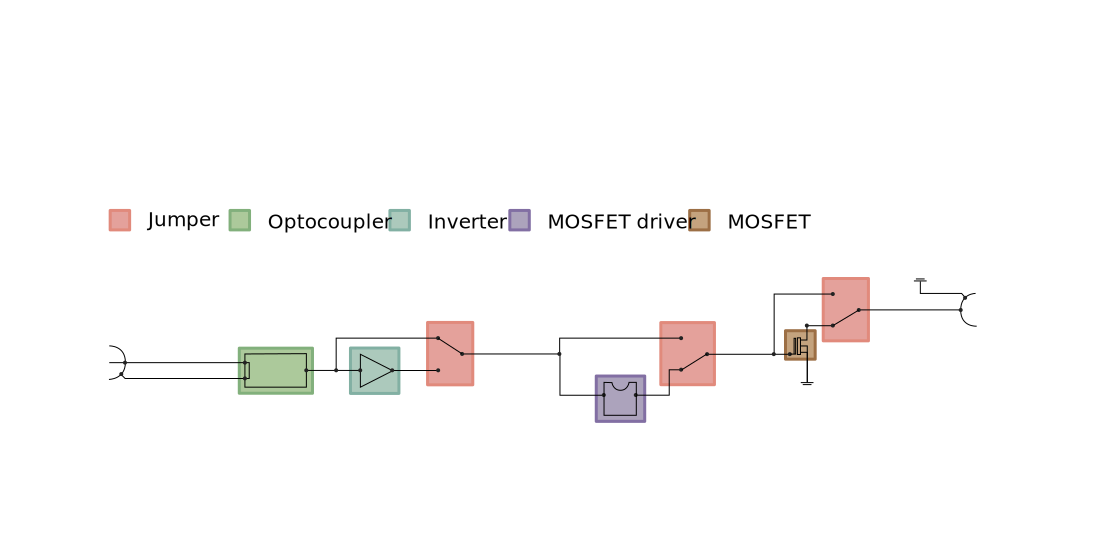
\includegraphics[width=1\textwidth]{drafts/shutter_circuit_simplified.pdf}
	\end{center}
}{shutter_circuit_simplified}{Electronic circuit to control the shutter}{
The first element in the circuit is the optocoupler which is used to decouple parts from the circuit in order to not create  loops, which would induce charges when the magnetic fields are on.
The remaining parts can be skipped, by setting the jumpers. The inverter will flip the sign on the voltage. The MOSFET driver is used in order to serve the correct voltage at the transistor's gate and to help during discharge, such that the MOSFET will not overheat. The transistor will finally serve a high current of \SI{2.5}{\ampere}, that is throughput to the shutter.
The jumpers in this figure are set as they are used in the experiment. The complete circuit can be found in \refAp{shutter_circuit}.
}

\newpage
\subsection{Dynamical properties}
The shutter operates by controlling a magnetic coil, which pulls a magnet. The magnet is reverted into its original position by a spring, closing the shutter. 
It was discussed before, in \refSubsec{shutter_electronic}, that more fans give a better approximation to a circular motion. Optimally, we would expect the shutter to open perfectly circular with linear velocity. Therefore, to optimize on this, one would look at opening and closing speeds, which should be minimal.

\label{subsec:shutter_dynamical}
\pltCustom{
	\begin{center}
		\includegraphics[width=0.8\textwidth]{drafts/shutter_experiment.pdf}
	\end{center}
	
	\begin{textblock}{2}(0.8,-2.55)
		\textbf{a.}
	\end{textblock}
	\begin{textblock}{2}(6.3,-2.55)
		\textbf{b.}
	\end{textblock}
}{shutter_experiment}{Probing the shutter for dynamics}{The shutter is proped at several positions using a laser. The offset in y direction was varied to find opening and closing times as a function of their offset.}

To find the actual dynamics of the shutter, an experiment was set up. The shutter was probed at several positions, using a laser, to find the opening time. An example of one of many measurements is shown in \refFig{shutterDiodeSignal}. The laser beam has a gaussian intensity distribution, which results in a error function on the photodiode as only partial intensiy is received from the diode, when the shutter is still blocking parts of the beam.

The points have been found by pointing a laser beam at a photodiode, which was blocked by the shutter. Since the laser has a finite radius, there is a transition in the signal from the minimum to the maximum, which is due to the approximately linear opening velocity of the shutter and the gaussian intensity distribution of the laser beam.

\plt{shutterDiodeSignal}{
	Shutter characterization}{The dynamics of the shutter were measured using a laser beam with a variable horizontal offset, which is fixed in this plot, and a photo diode measuring the laser intensity. In this figure, the offset is \SI{9.3}{\milli\meter} from the center. An error function was fitted yielding the time until the shutter opens. The opening time was hereby defined, where the error function has its mean value, in this example being \SI{5.2}{\volt}.
}

In order to find the opening and closing times of the shutter as seen in \refFig{shutterOpen}a., the offset from the centre of the shutter was varied. For larger offsets, the time from the initial trigger until a signal in the photodiode was received takes longer when the shutter is opening, while it takes shorter when it is closing.
In \refFig{shutterOpen}b. the speed is not perfectly linear. The deviations close to the centre originate from the shape of the fans. As there are five fans, there is no mirror symmetry, so that opening to the left and right is different in the end.

These measurements will later be used to time the triggers in the measurement, so that the shutter can stay closed as long as possible. But in order to optimize it, there were two shutters at hand, and several springs to choose from, the combination of which were all tested until the timings for opening $t_{open}=\SI{0.12}{\second}$ and for closing $t_{closing}=\SI{0.14}{\second}$ were found.

\pltCustom{
	\begin{center}
		%% Creator: Matplotlib, PGF backend
%%
%% To include the figure in your LaTeX document, write
%%   \input{<filename>.pgf}
%%
%% Make sure the required packages are loaded in your preamble
%%   \usepackage{pgf}
%%
%% Figures using additional raster images can only be included by \input if
%% they are in the same directory as the main LaTeX file. For loading figures
%% from other directories you can use the `import` package
%%   \usepackage{import}
%% and then include the figures with
%%   \import{<path to file>}{<filename>.pgf}
%%
%% Matplotlib used the following preamble
%%   \usepackage{fontspec}
%%   \setmainfont{DejaVu Serif}
%%   \setsansfont{DejaVu Sans}
%%   \setmonofont{DejaVu Sans Mono}
%%
\begingroup%
\makeatletter%
\begin{pgfpicture}%
\pgfpathrectangle{\pgfpointorigin}{\pgfqpoint{5.800000in}{1.792299in}}%
\pgfusepath{use as bounding box, clip}%
\begin{pgfscope}%
\pgfsetbuttcap%
\pgfsetmiterjoin%
\definecolor{currentfill}{rgb}{1.000000,1.000000,1.000000}%
\pgfsetfillcolor{currentfill}%
\pgfsetlinewidth{0.000000pt}%
\definecolor{currentstroke}{rgb}{1.000000,1.000000,1.000000}%
\pgfsetstrokecolor{currentstroke}%
\pgfsetdash{}{0pt}%
\pgfpathmoveto{\pgfqpoint{0.000000in}{0.000000in}}%
\pgfpathlineto{\pgfqpoint{5.800000in}{0.000000in}}%
\pgfpathlineto{\pgfqpoint{5.800000in}{1.792299in}}%
\pgfpathlineto{\pgfqpoint{0.000000in}{1.792299in}}%
\pgfpathclose%
\pgfusepath{fill}%
\end{pgfscope}%
\begin{pgfscope}%
\pgfsetbuttcap%
\pgfsetmiterjoin%
\definecolor{currentfill}{rgb}{1.000000,1.000000,1.000000}%
\pgfsetfillcolor{currentfill}%
\pgfsetlinewidth{0.000000pt}%
\definecolor{currentstroke}{rgb}{0.000000,0.000000,0.000000}%
\pgfsetstrokecolor{currentstroke}%
\pgfsetstrokeopacity{0.000000}%
\pgfsetdash{}{0pt}%
\pgfpathmoveto{\pgfqpoint{0.628675in}{0.451335in}}%
\pgfpathlineto{\pgfqpoint{2.840000in}{0.451335in}}%
\pgfpathlineto{\pgfqpoint{2.840000in}{1.620748in}}%
\pgfpathlineto{\pgfqpoint{0.628675in}{1.620748in}}%
\pgfpathclose%
\pgfusepath{fill}%
\end{pgfscope}%
\begin{pgfscope}%
\pgfpathrectangle{\pgfqpoint{0.628675in}{0.451335in}}{\pgfqpoint{2.211325in}{1.169413in}} %
\pgfusepath{clip}%
\pgfsetbuttcap%
\pgfsetroundjoin%
\pgfsetlinewidth{0.501875pt}%
\definecolor{currentstroke}{rgb}{0.000000,0.000000,1.000000}%
\pgfsetstrokecolor{currentstroke}%
\pgfsetdash{}{0pt}%
\pgfpathmoveto{\pgfqpoint{0.660265in}{1.532084in}}%
\pgfpathlineto{\pgfqpoint{0.660265in}{1.552070in}}%
\pgfusepath{stroke}%
\end{pgfscope}%
\begin{pgfscope}%
\pgfpathrectangle{\pgfqpoint{0.628675in}{0.451335in}}{\pgfqpoint{2.211325in}{1.169413in}} %
\pgfusepath{clip}%
\pgfsetbuttcap%
\pgfsetroundjoin%
\pgfsetlinewidth{0.501875pt}%
\definecolor{currentstroke}{rgb}{0.000000,0.000000,1.000000}%
\pgfsetstrokecolor{currentstroke}%
\pgfsetdash{}{0pt}%
\pgfpathmoveto{\pgfqpoint{0.723446in}{1.456610in}}%
\pgfpathlineto{\pgfqpoint{0.723446in}{1.484747in}}%
\pgfusepath{stroke}%
\end{pgfscope}%
\begin{pgfscope}%
\pgfpathrectangle{\pgfqpoint{0.628675in}{0.451335in}}{\pgfqpoint{2.211325in}{1.169413in}} %
\pgfusepath{clip}%
\pgfsetbuttcap%
\pgfsetroundjoin%
\pgfsetlinewidth{0.501875pt}%
\definecolor{currentstroke}{rgb}{0.000000,0.000000,1.000000}%
\pgfsetstrokecolor{currentstroke}%
\pgfsetdash{}{0pt}%
\pgfpathmoveto{\pgfqpoint{0.786627in}{1.406977in}}%
\pgfpathlineto{\pgfqpoint{0.786627in}{1.422434in}}%
\pgfusepath{stroke}%
\end{pgfscope}%
\begin{pgfscope}%
\pgfpathrectangle{\pgfqpoint{0.628675in}{0.451335in}}{\pgfqpoint{2.211325in}{1.169413in}} %
\pgfusepath{clip}%
\pgfsetbuttcap%
\pgfsetroundjoin%
\pgfsetlinewidth{0.501875pt}%
\definecolor{currentstroke}{rgb}{0.000000,0.000000,1.000000}%
\pgfsetstrokecolor{currentstroke}%
\pgfsetdash{}{0pt}%
\pgfpathmoveto{\pgfqpoint{0.849808in}{1.334617in}}%
\pgfpathlineto{\pgfqpoint{0.849808in}{1.357787in}}%
\pgfusepath{stroke}%
\end{pgfscope}%
\begin{pgfscope}%
\pgfpathrectangle{\pgfqpoint{0.628675in}{0.451335in}}{\pgfqpoint{2.211325in}{1.169413in}} %
\pgfusepath{clip}%
\pgfsetbuttcap%
\pgfsetroundjoin%
\pgfsetlinewidth{0.501875pt}%
\definecolor{currentstroke}{rgb}{0.000000,0.000000,1.000000}%
\pgfsetstrokecolor{currentstroke}%
\pgfsetdash{}{0pt}%
\pgfpathmoveto{\pgfqpoint{0.912988in}{1.263423in}}%
\pgfpathlineto{\pgfqpoint{0.912988in}{1.282027in}}%
\pgfusepath{stroke}%
\end{pgfscope}%
\begin{pgfscope}%
\pgfpathrectangle{\pgfqpoint{0.628675in}{0.451335in}}{\pgfqpoint{2.211325in}{1.169413in}} %
\pgfusepath{clip}%
\pgfsetbuttcap%
\pgfsetroundjoin%
\pgfsetlinewidth{0.501875pt}%
\definecolor{currentstroke}{rgb}{0.000000,0.000000,1.000000}%
\pgfsetstrokecolor{currentstroke}%
\pgfsetdash{}{0pt}%
\pgfpathmoveto{\pgfqpoint{0.976169in}{1.199524in}}%
\pgfpathlineto{\pgfqpoint{0.976169in}{1.223543in}}%
\pgfusepath{stroke}%
\end{pgfscope}%
\begin{pgfscope}%
\pgfpathrectangle{\pgfqpoint{0.628675in}{0.451335in}}{\pgfqpoint{2.211325in}{1.169413in}} %
\pgfusepath{clip}%
\pgfsetbuttcap%
\pgfsetroundjoin%
\pgfsetlinewidth{0.501875pt}%
\definecolor{currentstroke}{rgb}{0.000000,0.000000,1.000000}%
\pgfsetstrokecolor{currentstroke}%
\pgfsetdash{}{0pt}%
\pgfpathmoveto{\pgfqpoint{1.039350in}{1.134073in}}%
\pgfpathlineto{\pgfqpoint{1.039350in}{1.158137in}}%
\pgfusepath{stroke}%
\end{pgfscope}%
\begin{pgfscope}%
\pgfpathrectangle{\pgfqpoint{0.628675in}{0.451335in}}{\pgfqpoint{2.211325in}{1.169413in}} %
\pgfusepath{clip}%
\pgfsetbuttcap%
\pgfsetroundjoin%
\pgfsetlinewidth{0.501875pt}%
\definecolor{currentstroke}{rgb}{0.000000,0.000000,1.000000}%
\pgfsetstrokecolor{currentstroke}%
\pgfsetdash{}{0pt}%
\pgfpathmoveto{\pgfqpoint{1.102530in}{1.072872in}}%
\pgfpathlineto{\pgfqpoint{1.102530in}{1.089163in}}%
\pgfusepath{stroke}%
\end{pgfscope}%
\begin{pgfscope}%
\pgfpathrectangle{\pgfqpoint{0.628675in}{0.451335in}}{\pgfqpoint{2.211325in}{1.169413in}} %
\pgfusepath{clip}%
\pgfsetbuttcap%
\pgfsetroundjoin%
\pgfsetlinewidth{0.501875pt}%
\definecolor{currentstroke}{rgb}{0.000000,0.000000,1.000000}%
\pgfsetstrokecolor{currentstroke}%
\pgfsetdash{}{0pt}%
\pgfpathmoveto{\pgfqpoint{1.165711in}{0.996417in}}%
\pgfpathlineto{\pgfqpoint{1.165711in}{1.017825in}}%
\pgfusepath{stroke}%
\end{pgfscope}%
\begin{pgfscope}%
\pgfpathrectangle{\pgfqpoint{0.628675in}{0.451335in}}{\pgfqpoint{2.211325in}{1.169413in}} %
\pgfusepath{clip}%
\pgfsetbuttcap%
\pgfsetroundjoin%
\pgfsetlinewidth{0.501875pt}%
\definecolor{currentstroke}{rgb}{0.000000,0.000000,1.000000}%
\pgfsetstrokecolor{currentstroke}%
\pgfsetdash{}{0pt}%
\pgfpathmoveto{\pgfqpoint{1.228892in}{0.925479in}}%
\pgfpathlineto{\pgfqpoint{1.228892in}{0.946161in}}%
\pgfusepath{stroke}%
\end{pgfscope}%
\begin{pgfscope}%
\pgfpathrectangle{\pgfqpoint{0.628675in}{0.451335in}}{\pgfqpoint{2.211325in}{1.169413in}} %
\pgfusepath{clip}%
\pgfsetbuttcap%
\pgfsetroundjoin%
\pgfsetlinewidth{0.501875pt}%
\definecolor{currentstroke}{rgb}{0.000000,0.000000,1.000000}%
\pgfsetstrokecolor{currentstroke}%
\pgfsetdash{}{0pt}%
\pgfpathmoveto{\pgfqpoint{1.292073in}{0.853630in}}%
\pgfpathlineto{\pgfqpoint{1.292073in}{0.872007in}}%
\pgfusepath{stroke}%
\end{pgfscope}%
\begin{pgfscope}%
\pgfpathrectangle{\pgfqpoint{0.628675in}{0.451335in}}{\pgfqpoint{2.211325in}{1.169413in}} %
\pgfusepath{clip}%
\pgfsetbuttcap%
\pgfsetroundjoin%
\pgfsetlinewidth{0.501875pt}%
\definecolor{currentstroke}{rgb}{0.000000,0.000000,1.000000}%
\pgfsetstrokecolor{currentstroke}%
\pgfsetdash{}{0pt}%
\pgfpathmoveto{\pgfqpoint{1.355253in}{0.777121in}}%
\pgfpathlineto{\pgfqpoint{1.355253in}{0.796690in}}%
\pgfusepath{stroke}%
\end{pgfscope}%
\begin{pgfscope}%
\pgfpathrectangle{\pgfqpoint{0.628675in}{0.451335in}}{\pgfqpoint{2.211325in}{1.169413in}} %
\pgfusepath{clip}%
\pgfsetbuttcap%
\pgfsetroundjoin%
\pgfsetlinewidth{0.501875pt}%
\definecolor{currentstroke}{rgb}{0.000000,0.000000,1.000000}%
\pgfsetstrokecolor{currentstroke}%
\pgfsetdash{}{0pt}%
\pgfpathmoveto{\pgfqpoint{1.418434in}{0.731983in}}%
\pgfpathlineto{\pgfqpoint{1.418434in}{0.752589in}}%
\pgfusepath{stroke}%
\end{pgfscope}%
\begin{pgfscope}%
\pgfpathrectangle{\pgfqpoint{0.628675in}{0.451335in}}{\pgfqpoint{2.211325in}{1.169413in}} %
\pgfusepath{clip}%
\pgfsetbuttcap%
\pgfsetroundjoin%
\pgfsetlinewidth{0.501875pt}%
\definecolor{currentstroke}{rgb}{0.000000,0.000000,1.000000}%
\pgfsetstrokecolor{currentstroke}%
\pgfsetdash{}{0pt}%
\pgfpathmoveto{\pgfqpoint{1.481615in}{0.612286in}}%
\pgfpathlineto{\pgfqpoint{1.481615in}{0.631497in}}%
\pgfusepath{stroke}%
\end{pgfscope}%
\begin{pgfscope}%
\pgfpathrectangle{\pgfqpoint{0.628675in}{0.451335in}}{\pgfqpoint{2.211325in}{1.169413in}} %
\pgfusepath{clip}%
\pgfsetbuttcap%
\pgfsetroundjoin%
\pgfsetlinewidth{0.501875pt}%
\definecolor{currentstroke}{rgb}{0.000000,0.000000,1.000000}%
\pgfsetstrokecolor{currentstroke}%
\pgfsetdash{}{0pt}%
\pgfpathmoveto{\pgfqpoint{1.544795in}{0.508530in}}%
\pgfpathlineto{\pgfqpoint{1.544795in}{0.531987in}}%
\pgfusepath{stroke}%
\end{pgfscope}%
\begin{pgfscope}%
\pgfpathrectangle{\pgfqpoint{0.628675in}{0.451335in}}{\pgfqpoint{2.211325in}{1.169413in}} %
\pgfusepath{clip}%
\pgfsetbuttcap%
\pgfsetroundjoin%
\pgfsetlinewidth{0.501875pt}%
\definecolor{currentstroke}{rgb}{0.000000,0.000000,1.000000}%
\pgfsetstrokecolor{currentstroke}%
\pgfsetdash{}{0pt}%
\pgfpathmoveto{\pgfqpoint{1.607976in}{0.496512in}}%
\pgfpathlineto{\pgfqpoint{1.607976in}{0.513718in}}%
\pgfusepath{stroke}%
\end{pgfscope}%
\begin{pgfscope}%
\pgfpathrectangle{\pgfqpoint{0.628675in}{0.451335in}}{\pgfqpoint{2.211325in}{1.169413in}} %
\pgfusepath{clip}%
\pgfsetbuttcap%
\pgfsetroundjoin%
\pgfsetlinewidth{0.501875pt}%
\definecolor{currentstroke}{rgb}{0.000000,0.000000,1.000000}%
\pgfsetstrokecolor{currentstroke}%
\pgfsetdash{}{0pt}%
\pgfpathmoveto{\pgfqpoint{1.671157in}{0.494199in}}%
\pgfpathlineto{\pgfqpoint{1.671157in}{0.506500in}}%
\pgfusepath{stroke}%
\end{pgfscope}%
\begin{pgfscope}%
\pgfpathrectangle{\pgfqpoint{0.628675in}{0.451335in}}{\pgfqpoint{2.211325in}{1.169413in}} %
\pgfusepath{clip}%
\pgfsetbuttcap%
\pgfsetroundjoin%
\pgfsetlinewidth{0.501875pt}%
\definecolor{currentstroke}{rgb}{0.000000,0.000000,1.000000}%
\pgfsetstrokecolor{currentstroke}%
\pgfsetdash{}{0pt}%
\pgfpathmoveto{\pgfqpoint{1.734338in}{0.569858in}}%
\pgfpathlineto{\pgfqpoint{1.734338in}{0.588419in}}%
\pgfusepath{stroke}%
\end{pgfscope}%
\begin{pgfscope}%
\pgfpathrectangle{\pgfqpoint{0.628675in}{0.451335in}}{\pgfqpoint{2.211325in}{1.169413in}} %
\pgfusepath{clip}%
\pgfsetbuttcap%
\pgfsetroundjoin%
\pgfsetlinewidth{0.501875pt}%
\definecolor{currentstroke}{rgb}{0.000000,0.000000,1.000000}%
\pgfsetstrokecolor{currentstroke}%
\pgfsetdash{}{0pt}%
\pgfpathmoveto{\pgfqpoint{1.797518in}{0.631442in}}%
\pgfpathlineto{\pgfqpoint{1.797518in}{0.643501in}}%
\pgfusepath{stroke}%
\end{pgfscope}%
\begin{pgfscope}%
\pgfpathrectangle{\pgfqpoint{0.628675in}{0.451335in}}{\pgfqpoint{2.211325in}{1.169413in}} %
\pgfusepath{clip}%
\pgfsetbuttcap%
\pgfsetroundjoin%
\pgfsetlinewidth{0.501875pt}%
\definecolor{currentstroke}{rgb}{0.000000,0.000000,1.000000}%
\pgfsetstrokecolor{currentstroke}%
\pgfsetdash{}{0pt}%
\pgfpathmoveto{\pgfqpoint{1.860699in}{0.670278in}}%
\pgfpathlineto{\pgfqpoint{1.860699in}{0.682391in}}%
\pgfusepath{stroke}%
\end{pgfscope}%
\begin{pgfscope}%
\pgfpathrectangle{\pgfqpoint{0.628675in}{0.451335in}}{\pgfqpoint{2.211325in}{1.169413in}} %
\pgfusepath{clip}%
\pgfsetbuttcap%
\pgfsetroundjoin%
\pgfsetlinewidth{0.501875pt}%
\definecolor{currentstroke}{rgb}{0.000000,0.000000,1.000000}%
\pgfsetstrokecolor{currentstroke}%
\pgfsetdash{}{0pt}%
\pgfpathmoveto{\pgfqpoint{1.923880in}{0.709878in}}%
\pgfpathlineto{\pgfqpoint{1.923880in}{0.726082in}}%
\pgfusepath{stroke}%
\end{pgfscope}%
\begin{pgfscope}%
\pgfpathrectangle{\pgfqpoint{0.628675in}{0.451335in}}{\pgfqpoint{2.211325in}{1.169413in}} %
\pgfusepath{clip}%
\pgfsetbuttcap%
\pgfsetroundjoin%
\pgfsetlinewidth{0.501875pt}%
\definecolor{currentstroke}{rgb}{0.000000,0.000000,1.000000}%
\pgfsetstrokecolor{currentstroke}%
\pgfsetdash{}{0pt}%
\pgfpathmoveto{\pgfqpoint{1.987060in}{0.759366in}}%
\pgfpathlineto{\pgfqpoint{1.987060in}{0.778707in}}%
\pgfusepath{stroke}%
\end{pgfscope}%
\begin{pgfscope}%
\pgfpathrectangle{\pgfqpoint{0.628675in}{0.451335in}}{\pgfqpoint{2.211325in}{1.169413in}} %
\pgfusepath{clip}%
\pgfsetbuttcap%
\pgfsetroundjoin%
\pgfsetlinewidth{0.501875pt}%
\definecolor{currentstroke}{rgb}{0.000000,0.000000,1.000000}%
\pgfsetstrokecolor{currentstroke}%
\pgfsetdash{}{0pt}%
\pgfpathmoveto{\pgfqpoint{2.050241in}{0.805612in}}%
\pgfpathlineto{\pgfqpoint{2.050241in}{0.836861in}}%
\pgfusepath{stroke}%
\end{pgfscope}%
\begin{pgfscope}%
\pgfpathrectangle{\pgfqpoint{0.628675in}{0.451335in}}{\pgfqpoint{2.211325in}{1.169413in}} %
\pgfusepath{clip}%
\pgfsetbuttcap%
\pgfsetroundjoin%
\pgfsetlinewidth{0.501875pt}%
\definecolor{currentstroke}{rgb}{0.000000,0.000000,1.000000}%
\pgfsetstrokecolor{currentstroke}%
\pgfsetdash{}{0pt}%
\pgfpathmoveto{\pgfqpoint{2.113422in}{0.865436in}}%
\pgfpathlineto{\pgfqpoint{2.113422in}{0.889474in}}%
\pgfusepath{stroke}%
\end{pgfscope}%
\begin{pgfscope}%
\pgfpathrectangle{\pgfqpoint{0.628675in}{0.451335in}}{\pgfqpoint{2.211325in}{1.169413in}} %
\pgfusepath{clip}%
\pgfsetbuttcap%
\pgfsetroundjoin%
\pgfsetlinewidth{0.501875pt}%
\definecolor{currentstroke}{rgb}{0.000000,0.000000,1.000000}%
\pgfsetstrokecolor{currentstroke}%
\pgfsetdash{}{0pt}%
\pgfpathmoveto{\pgfqpoint{2.176603in}{0.924612in}}%
\pgfpathlineto{\pgfqpoint{2.176603in}{0.952470in}}%
\pgfusepath{stroke}%
\end{pgfscope}%
\begin{pgfscope}%
\pgfpathrectangle{\pgfqpoint{0.628675in}{0.451335in}}{\pgfqpoint{2.211325in}{1.169413in}} %
\pgfusepath{clip}%
\pgfsetbuttcap%
\pgfsetroundjoin%
\pgfsetlinewidth{0.501875pt}%
\definecolor{currentstroke}{rgb}{0.000000,0.000000,1.000000}%
\pgfsetstrokecolor{currentstroke}%
\pgfsetdash{}{0pt}%
\pgfpathmoveto{\pgfqpoint{2.239783in}{0.990427in}}%
\pgfpathlineto{\pgfqpoint{2.239783in}{1.008313in}}%
\pgfusepath{stroke}%
\end{pgfscope}%
\begin{pgfscope}%
\pgfpathrectangle{\pgfqpoint{0.628675in}{0.451335in}}{\pgfqpoint{2.211325in}{1.169413in}} %
\pgfusepath{clip}%
\pgfsetbuttcap%
\pgfsetroundjoin%
\pgfsetlinewidth{0.501875pt}%
\definecolor{currentstroke}{rgb}{0.000000,0.000000,1.000000}%
\pgfsetstrokecolor{currentstroke}%
\pgfsetdash{}{0pt}%
\pgfpathmoveto{\pgfqpoint{2.302964in}{1.048660in}}%
\pgfpathlineto{\pgfqpoint{2.302964in}{1.070609in}}%
\pgfusepath{stroke}%
\end{pgfscope}%
\begin{pgfscope}%
\pgfpathrectangle{\pgfqpoint{0.628675in}{0.451335in}}{\pgfqpoint{2.211325in}{1.169413in}} %
\pgfusepath{clip}%
\pgfsetbuttcap%
\pgfsetroundjoin%
\pgfsetlinewidth{0.501875pt}%
\definecolor{currentstroke}{rgb}{0.000000,0.000000,1.000000}%
\pgfsetstrokecolor{currentstroke}%
\pgfsetdash{}{0pt}%
\pgfpathmoveto{\pgfqpoint{2.366145in}{1.120684in}}%
\pgfpathlineto{\pgfqpoint{2.366145in}{1.140596in}}%
\pgfusepath{stroke}%
\end{pgfscope}%
\begin{pgfscope}%
\pgfpathrectangle{\pgfqpoint{0.628675in}{0.451335in}}{\pgfqpoint{2.211325in}{1.169413in}} %
\pgfusepath{clip}%
\pgfsetbuttcap%
\pgfsetroundjoin%
\pgfsetlinewidth{0.501875pt}%
\definecolor{currentstroke}{rgb}{0.000000,0.000000,1.000000}%
\pgfsetstrokecolor{currentstroke}%
\pgfsetdash{}{0pt}%
\pgfpathmoveto{\pgfqpoint{2.429325in}{1.189636in}}%
\pgfpathlineto{\pgfqpoint{2.429325in}{1.210873in}}%
\pgfusepath{stroke}%
\end{pgfscope}%
\begin{pgfscope}%
\pgfpathrectangle{\pgfqpoint{0.628675in}{0.451335in}}{\pgfqpoint{2.211325in}{1.169413in}} %
\pgfusepath{clip}%
\pgfsetbuttcap%
\pgfsetroundjoin%
\pgfsetlinewidth{0.501875pt}%
\definecolor{currentstroke}{rgb}{0.000000,0.000000,1.000000}%
\pgfsetstrokecolor{currentstroke}%
\pgfsetdash{}{0pt}%
\pgfpathmoveto{\pgfqpoint{2.492506in}{1.257851in}}%
\pgfpathlineto{\pgfqpoint{2.492506in}{1.282203in}}%
\pgfusepath{stroke}%
\end{pgfscope}%
\begin{pgfscope}%
\pgfpathrectangle{\pgfqpoint{0.628675in}{0.451335in}}{\pgfqpoint{2.211325in}{1.169413in}} %
\pgfusepath{clip}%
\pgfsetbuttcap%
\pgfsetroundjoin%
\pgfsetlinewidth{0.501875pt}%
\definecolor{currentstroke}{rgb}{0.000000,0.000000,1.000000}%
\pgfsetstrokecolor{currentstroke}%
\pgfsetdash{}{0pt}%
\pgfpathmoveto{\pgfqpoint{2.555687in}{1.324354in}}%
\pgfpathlineto{\pgfqpoint{2.555687in}{1.349603in}}%
\pgfusepath{stroke}%
\end{pgfscope}%
\begin{pgfscope}%
\pgfpathrectangle{\pgfqpoint{0.628675in}{0.451335in}}{\pgfqpoint{2.211325in}{1.169413in}} %
\pgfusepath{clip}%
\pgfsetbuttcap%
\pgfsetroundjoin%
\pgfsetlinewidth{0.501875pt}%
\definecolor{currentstroke}{rgb}{0.000000,0.000000,1.000000}%
\pgfsetstrokecolor{currentstroke}%
\pgfsetdash{}{0pt}%
\pgfpathmoveto{\pgfqpoint{2.618868in}{1.402151in}}%
\pgfpathlineto{\pgfqpoint{2.618868in}{1.429936in}}%
\pgfusepath{stroke}%
\end{pgfscope}%
\begin{pgfscope}%
\pgfpathrectangle{\pgfqpoint{0.628675in}{0.451335in}}{\pgfqpoint{2.211325in}{1.169413in}} %
\pgfusepath{clip}%
\pgfsetbuttcap%
\pgfsetroundjoin%
\pgfsetlinewidth{0.501875pt}%
\definecolor{currentstroke}{rgb}{0.000000,0.000000,1.000000}%
\pgfsetstrokecolor{currentstroke}%
\pgfsetdash{}{0pt}%
\pgfpathmoveto{\pgfqpoint{2.682048in}{1.482921in}}%
\pgfpathlineto{\pgfqpoint{2.682048in}{1.507846in}}%
\pgfusepath{stroke}%
\end{pgfscope}%
\begin{pgfscope}%
\pgfpathrectangle{\pgfqpoint{0.628675in}{0.451335in}}{\pgfqpoint{2.211325in}{1.169413in}} %
\pgfusepath{clip}%
\pgfsetbuttcap%
\pgfsetroundjoin%
\pgfsetlinewidth{0.501875pt}%
\definecolor{currentstroke}{rgb}{0.000000,0.000000,1.000000}%
\pgfsetstrokecolor{currentstroke}%
\pgfsetdash{}{0pt}%
\pgfpathmoveto{\pgfqpoint{2.745229in}{1.559556in}}%
\pgfpathlineto{\pgfqpoint{2.745229in}{1.584586in}}%
\pgfusepath{stroke}%
\end{pgfscope}%
\begin{pgfscope}%
\pgfpathrectangle{\pgfqpoint{0.628675in}{0.451335in}}{\pgfqpoint{2.211325in}{1.169413in}} %
\pgfusepath{clip}%
\pgfsetbuttcap%
\pgfsetroundjoin%
\definecolor{currentfill}{rgb}{0.000000,0.000000,1.000000}%
\pgfsetfillcolor{currentfill}%
\pgfsetlinewidth{0.501875pt}%
\definecolor{currentstroke}{rgb}{0.000000,0.000000,1.000000}%
\pgfsetstrokecolor{currentstroke}%
\pgfsetdash{}{0pt}%
\pgfsys@defobject{currentmarker}{\pgfqpoint{-0.011111in}{-0.000000in}}{\pgfqpoint{0.011111in}{0.000000in}}{%
\pgfpathmoveto{\pgfqpoint{0.011111in}{-0.000000in}}%
\pgfpathlineto{\pgfqpoint{-0.011111in}{0.000000in}}%
\pgfusepath{stroke,fill}%
}%
\begin{pgfscope}%
\pgfsys@transformshift{0.660265in}{1.532084in}%
\pgfsys@useobject{currentmarker}{}%
\end{pgfscope}%
\begin{pgfscope}%
\pgfsys@transformshift{0.723446in}{1.456610in}%
\pgfsys@useobject{currentmarker}{}%
\end{pgfscope}%
\begin{pgfscope}%
\pgfsys@transformshift{0.786627in}{1.406977in}%
\pgfsys@useobject{currentmarker}{}%
\end{pgfscope}%
\begin{pgfscope}%
\pgfsys@transformshift{0.849808in}{1.334617in}%
\pgfsys@useobject{currentmarker}{}%
\end{pgfscope}%
\begin{pgfscope}%
\pgfsys@transformshift{0.912988in}{1.263423in}%
\pgfsys@useobject{currentmarker}{}%
\end{pgfscope}%
\begin{pgfscope}%
\pgfsys@transformshift{0.976169in}{1.199524in}%
\pgfsys@useobject{currentmarker}{}%
\end{pgfscope}%
\begin{pgfscope}%
\pgfsys@transformshift{1.039350in}{1.134073in}%
\pgfsys@useobject{currentmarker}{}%
\end{pgfscope}%
\begin{pgfscope}%
\pgfsys@transformshift{1.102530in}{1.072872in}%
\pgfsys@useobject{currentmarker}{}%
\end{pgfscope}%
\begin{pgfscope}%
\pgfsys@transformshift{1.165711in}{0.996417in}%
\pgfsys@useobject{currentmarker}{}%
\end{pgfscope}%
\begin{pgfscope}%
\pgfsys@transformshift{1.228892in}{0.925479in}%
\pgfsys@useobject{currentmarker}{}%
\end{pgfscope}%
\begin{pgfscope}%
\pgfsys@transformshift{1.292073in}{0.853630in}%
\pgfsys@useobject{currentmarker}{}%
\end{pgfscope}%
\begin{pgfscope}%
\pgfsys@transformshift{1.355253in}{0.777121in}%
\pgfsys@useobject{currentmarker}{}%
\end{pgfscope}%
\begin{pgfscope}%
\pgfsys@transformshift{1.418434in}{0.731983in}%
\pgfsys@useobject{currentmarker}{}%
\end{pgfscope}%
\begin{pgfscope}%
\pgfsys@transformshift{1.481615in}{0.612286in}%
\pgfsys@useobject{currentmarker}{}%
\end{pgfscope}%
\begin{pgfscope}%
\pgfsys@transformshift{1.544795in}{0.508530in}%
\pgfsys@useobject{currentmarker}{}%
\end{pgfscope}%
\begin{pgfscope}%
\pgfsys@transformshift{1.607976in}{0.496512in}%
\pgfsys@useobject{currentmarker}{}%
\end{pgfscope}%
\begin{pgfscope}%
\pgfsys@transformshift{1.671157in}{0.494199in}%
\pgfsys@useobject{currentmarker}{}%
\end{pgfscope}%
\begin{pgfscope}%
\pgfsys@transformshift{1.734338in}{0.569858in}%
\pgfsys@useobject{currentmarker}{}%
\end{pgfscope}%
\begin{pgfscope}%
\pgfsys@transformshift{1.797518in}{0.631442in}%
\pgfsys@useobject{currentmarker}{}%
\end{pgfscope}%
\begin{pgfscope}%
\pgfsys@transformshift{1.860699in}{0.670278in}%
\pgfsys@useobject{currentmarker}{}%
\end{pgfscope}%
\begin{pgfscope}%
\pgfsys@transformshift{1.923880in}{0.709878in}%
\pgfsys@useobject{currentmarker}{}%
\end{pgfscope}%
\begin{pgfscope}%
\pgfsys@transformshift{1.987060in}{0.759366in}%
\pgfsys@useobject{currentmarker}{}%
\end{pgfscope}%
\begin{pgfscope}%
\pgfsys@transformshift{2.050241in}{0.805612in}%
\pgfsys@useobject{currentmarker}{}%
\end{pgfscope}%
\begin{pgfscope}%
\pgfsys@transformshift{2.113422in}{0.865436in}%
\pgfsys@useobject{currentmarker}{}%
\end{pgfscope}%
\begin{pgfscope}%
\pgfsys@transformshift{2.176603in}{0.924612in}%
\pgfsys@useobject{currentmarker}{}%
\end{pgfscope}%
\begin{pgfscope}%
\pgfsys@transformshift{2.239783in}{0.990427in}%
\pgfsys@useobject{currentmarker}{}%
\end{pgfscope}%
\begin{pgfscope}%
\pgfsys@transformshift{2.302964in}{1.048660in}%
\pgfsys@useobject{currentmarker}{}%
\end{pgfscope}%
\begin{pgfscope}%
\pgfsys@transformshift{2.366145in}{1.120684in}%
\pgfsys@useobject{currentmarker}{}%
\end{pgfscope}%
\begin{pgfscope}%
\pgfsys@transformshift{2.429325in}{1.189636in}%
\pgfsys@useobject{currentmarker}{}%
\end{pgfscope}%
\begin{pgfscope}%
\pgfsys@transformshift{2.492506in}{1.257851in}%
\pgfsys@useobject{currentmarker}{}%
\end{pgfscope}%
\begin{pgfscope}%
\pgfsys@transformshift{2.555687in}{1.324354in}%
\pgfsys@useobject{currentmarker}{}%
\end{pgfscope}%
\begin{pgfscope}%
\pgfsys@transformshift{2.618868in}{1.402151in}%
\pgfsys@useobject{currentmarker}{}%
\end{pgfscope}%
\begin{pgfscope}%
\pgfsys@transformshift{2.682048in}{1.482921in}%
\pgfsys@useobject{currentmarker}{}%
\end{pgfscope}%
\begin{pgfscope}%
\pgfsys@transformshift{2.745229in}{1.559556in}%
\pgfsys@useobject{currentmarker}{}%
\end{pgfscope}%
\end{pgfscope}%
\begin{pgfscope}%
\pgfpathrectangle{\pgfqpoint{0.628675in}{0.451335in}}{\pgfqpoint{2.211325in}{1.169413in}} %
\pgfusepath{clip}%
\pgfsetbuttcap%
\pgfsetroundjoin%
\definecolor{currentfill}{rgb}{0.000000,0.000000,1.000000}%
\pgfsetfillcolor{currentfill}%
\pgfsetlinewidth{0.501875pt}%
\definecolor{currentstroke}{rgb}{0.000000,0.000000,1.000000}%
\pgfsetstrokecolor{currentstroke}%
\pgfsetdash{}{0pt}%
\pgfsys@defobject{currentmarker}{\pgfqpoint{-0.011111in}{-0.000000in}}{\pgfqpoint{0.011111in}{0.000000in}}{%
\pgfpathmoveto{\pgfqpoint{0.011111in}{-0.000000in}}%
\pgfpathlineto{\pgfqpoint{-0.011111in}{0.000000in}}%
\pgfusepath{stroke,fill}%
}%
\begin{pgfscope}%
\pgfsys@transformshift{0.660265in}{1.552070in}%
\pgfsys@useobject{currentmarker}{}%
\end{pgfscope}%
\begin{pgfscope}%
\pgfsys@transformshift{0.723446in}{1.484747in}%
\pgfsys@useobject{currentmarker}{}%
\end{pgfscope}%
\begin{pgfscope}%
\pgfsys@transformshift{0.786627in}{1.422434in}%
\pgfsys@useobject{currentmarker}{}%
\end{pgfscope}%
\begin{pgfscope}%
\pgfsys@transformshift{0.849808in}{1.357787in}%
\pgfsys@useobject{currentmarker}{}%
\end{pgfscope}%
\begin{pgfscope}%
\pgfsys@transformshift{0.912988in}{1.282027in}%
\pgfsys@useobject{currentmarker}{}%
\end{pgfscope}%
\begin{pgfscope}%
\pgfsys@transformshift{0.976169in}{1.223543in}%
\pgfsys@useobject{currentmarker}{}%
\end{pgfscope}%
\begin{pgfscope}%
\pgfsys@transformshift{1.039350in}{1.158137in}%
\pgfsys@useobject{currentmarker}{}%
\end{pgfscope}%
\begin{pgfscope}%
\pgfsys@transformshift{1.102530in}{1.089163in}%
\pgfsys@useobject{currentmarker}{}%
\end{pgfscope}%
\begin{pgfscope}%
\pgfsys@transformshift{1.165711in}{1.017825in}%
\pgfsys@useobject{currentmarker}{}%
\end{pgfscope}%
\begin{pgfscope}%
\pgfsys@transformshift{1.228892in}{0.946161in}%
\pgfsys@useobject{currentmarker}{}%
\end{pgfscope}%
\begin{pgfscope}%
\pgfsys@transformshift{1.292073in}{0.872007in}%
\pgfsys@useobject{currentmarker}{}%
\end{pgfscope}%
\begin{pgfscope}%
\pgfsys@transformshift{1.355253in}{0.796690in}%
\pgfsys@useobject{currentmarker}{}%
\end{pgfscope}%
\begin{pgfscope}%
\pgfsys@transformshift{1.418434in}{0.752589in}%
\pgfsys@useobject{currentmarker}{}%
\end{pgfscope}%
\begin{pgfscope}%
\pgfsys@transformshift{1.481615in}{0.631497in}%
\pgfsys@useobject{currentmarker}{}%
\end{pgfscope}%
\begin{pgfscope}%
\pgfsys@transformshift{1.544795in}{0.531987in}%
\pgfsys@useobject{currentmarker}{}%
\end{pgfscope}%
\begin{pgfscope}%
\pgfsys@transformshift{1.607976in}{0.513718in}%
\pgfsys@useobject{currentmarker}{}%
\end{pgfscope}%
\begin{pgfscope}%
\pgfsys@transformshift{1.671157in}{0.506500in}%
\pgfsys@useobject{currentmarker}{}%
\end{pgfscope}%
\begin{pgfscope}%
\pgfsys@transformshift{1.734338in}{0.588419in}%
\pgfsys@useobject{currentmarker}{}%
\end{pgfscope}%
\begin{pgfscope}%
\pgfsys@transformshift{1.797518in}{0.643501in}%
\pgfsys@useobject{currentmarker}{}%
\end{pgfscope}%
\begin{pgfscope}%
\pgfsys@transformshift{1.860699in}{0.682391in}%
\pgfsys@useobject{currentmarker}{}%
\end{pgfscope}%
\begin{pgfscope}%
\pgfsys@transformshift{1.923880in}{0.726082in}%
\pgfsys@useobject{currentmarker}{}%
\end{pgfscope}%
\begin{pgfscope}%
\pgfsys@transformshift{1.987060in}{0.778707in}%
\pgfsys@useobject{currentmarker}{}%
\end{pgfscope}%
\begin{pgfscope}%
\pgfsys@transformshift{2.050241in}{0.836861in}%
\pgfsys@useobject{currentmarker}{}%
\end{pgfscope}%
\begin{pgfscope}%
\pgfsys@transformshift{2.113422in}{0.889474in}%
\pgfsys@useobject{currentmarker}{}%
\end{pgfscope}%
\begin{pgfscope}%
\pgfsys@transformshift{2.176603in}{0.952470in}%
\pgfsys@useobject{currentmarker}{}%
\end{pgfscope}%
\begin{pgfscope}%
\pgfsys@transformshift{2.239783in}{1.008313in}%
\pgfsys@useobject{currentmarker}{}%
\end{pgfscope}%
\begin{pgfscope}%
\pgfsys@transformshift{2.302964in}{1.070609in}%
\pgfsys@useobject{currentmarker}{}%
\end{pgfscope}%
\begin{pgfscope}%
\pgfsys@transformshift{2.366145in}{1.140596in}%
\pgfsys@useobject{currentmarker}{}%
\end{pgfscope}%
\begin{pgfscope}%
\pgfsys@transformshift{2.429325in}{1.210873in}%
\pgfsys@useobject{currentmarker}{}%
\end{pgfscope}%
\begin{pgfscope}%
\pgfsys@transformshift{2.492506in}{1.282203in}%
\pgfsys@useobject{currentmarker}{}%
\end{pgfscope}%
\begin{pgfscope}%
\pgfsys@transformshift{2.555687in}{1.349603in}%
\pgfsys@useobject{currentmarker}{}%
\end{pgfscope}%
\begin{pgfscope}%
\pgfsys@transformshift{2.618868in}{1.429936in}%
\pgfsys@useobject{currentmarker}{}%
\end{pgfscope}%
\begin{pgfscope}%
\pgfsys@transformshift{2.682048in}{1.507846in}%
\pgfsys@useobject{currentmarker}{}%
\end{pgfscope}%
\begin{pgfscope}%
\pgfsys@transformshift{2.745229in}{1.584586in}%
\pgfsys@useobject{currentmarker}{}%
\end{pgfscope}%
\end{pgfscope}%
\begin{pgfscope}%
\pgfsetrectcap%
\pgfsetmiterjoin%
\pgfsetlinewidth{0.501875pt}%
\definecolor{currentstroke}{rgb}{0.000000,0.000000,0.000000}%
\pgfsetstrokecolor{currentstroke}%
\pgfsetdash{}{0pt}%
\pgfpathmoveto{\pgfqpoint{0.628675in}{0.451335in}}%
\pgfpathlineto{\pgfqpoint{2.840000in}{0.451335in}}%
\pgfusepath{stroke}%
\end{pgfscope}%
\begin{pgfscope}%
\pgfsetrectcap%
\pgfsetmiterjoin%
\pgfsetlinewidth{0.501875pt}%
\definecolor{currentstroke}{rgb}{0.000000,0.000000,0.000000}%
\pgfsetstrokecolor{currentstroke}%
\pgfsetdash{}{0pt}%
\pgfpathmoveto{\pgfqpoint{0.628675in}{0.451335in}}%
\pgfpathlineto{\pgfqpoint{0.628675in}{1.620748in}}%
\pgfusepath{stroke}%
\end{pgfscope}%
\begin{pgfscope}%
\pgfsetbuttcap%
\pgfsetroundjoin%
\definecolor{currentfill}{rgb}{0.000000,0.000000,0.000000}%
\pgfsetfillcolor{currentfill}%
\pgfsetlinewidth{0.501875pt}%
\definecolor{currentstroke}{rgb}{0.000000,0.000000,0.000000}%
\pgfsetstrokecolor{currentstroke}%
\pgfsetdash{}{0pt}%
\pgfsys@defobject{currentmarker}{\pgfqpoint{0.000000in}{-0.055556in}}{\pgfqpoint{0.000000in}{0.000000in}}{%
\pgfpathmoveto{\pgfqpoint{0.000000in}{0.000000in}}%
\pgfpathlineto{\pgfqpoint{0.000000in}{-0.055556in}}%
\pgfusepath{stroke,fill}%
}%
\begin{pgfscope}%
\pgfsys@transformshift{0.628675in}{0.451335in}%
\pgfsys@useobject{currentmarker}{}%
\end{pgfscope}%
\end{pgfscope}%
\begin{pgfscope}%
\pgftext[x=0.628675in,y=0.340224in,,top]{\rmfamily\fontsize{8.000000}{9.600000}\selectfont \(\displaystyle 5\)}%
\end{pgfscope}%
\begin{pgfscope}%
\pgfsetbuttcap%
\pgfsetroundjoin%
\definecolor{currentfill}{rgb}{0.000000,0.000000,0.000000}%
\pgfsetfillcolor{currentfill}%
\pgfsetlinewidth{0.501875pt}%
\definecolor{currentstroke}{rgb}{0.000000,0.000000,0.000000}%
\pgfsetstrokecolor{currentstroke}%
\pgfsetdash{}{0pt}%
\pgfsys@defobject{currentmarker}{\pgfqpoint{0.000000in}{-0.055556in}}{\pgfqpoint{0.000000in}{0.000000in}}{%
\pgfpathmoveto{\pgfqpoint{0.000000in}{0.000000in}}%
\pgfpathlineto{\pgfqpoint{0.000000in}{-0.055556in}}%
\pgfusepath{stroke,fill}%
}%
\begin{pgfscope}%
\pgfsys@transformshift{0.944579in}{0.451335in}%
\pgfsys@useobject{currentmarker}{}%
\end{pgfscope}%
\end{pgfscope}%
\begin{pgfscope}%
\pgftext[x=0.944579in,y=0.340224in,,top]{\rmfamily\fontsize{8.000000}{9.600000}\selectfont \(\displaystyle 10\)}%
\end{pgfscope}%
\begin{pgfscope}%
\pgfsetbuttcap%
\pgfsetroundjoin%
\definecolor{currentfill}{rgb}{0.000000,0.000000,0.000000}%
\pgfsetfillcolor{currentfill}%
\pgfsetlinewidth{0.501875pt}%
\definecolor{currentstroke}{rgb}{0.000000,0.000000,0.000000}%
\pgfsetstrokecolor{currentstroke}%
\pgfsetdash{}{0pt}%
\pgfsys@defobject{currentmarker}{\pgfqpoint{0.000000in}{-0.055556in}}{\pgfqpoint{0.000000in}{0.000000in}}{%
\pgfpathmoveto{\pgfqpoint{0.000000in}{0.000000in}}%
\pgfpathlineto{\pgfqpoint{0.000000in}{-0.055556in}}%
\pgfusepath{stroke,fill}%
}%
\begin{pgfscope}%
\pgfsys@transformshift{1.260482in}{0.451335in}%
\pgfsys@useobject{currentmarker}{}%
\end{pgfscope}%
\end{pgfscope}%
\begin{pgfscope}%
\pgftext[x=1.260482in,y=0.340224in,,top]{\rmfamily\fontsize{8.000000}{9.600000}\selectfont \(\displaystyle 15\)}%
\end{pgfscope}%
\begin{pgfscope}%
\pgfsetbuttcap%
\pgfsetroundjoin%
\definecolor{currentfill}{rgb}{0.000000,0.000000,0.000000}%
\pgfsetfillcolor{currentfill}%
\pgfsetlinewidth{0.501875pt}%
\definecolor{currentstroke}{rgb}{0.000000,0.000000,0.000000}%
\pgfsetstrokecolor{currentstroke}%
\pgfsetdash{}{0pt}%
\pgfsys@defobject{currentmarker}{\pgfqpoint{0.000000in}{-0.055556in}}{\pgfqpoint{0.000000in}{0.000000in}}{%
\pgfpathmoveto{\pgfqpoint{0.000000in}{0.000000in}}%
\pgfpathlineto{\pgfqpoint{0.000000in}{-0.055556in}}%
\pgfusepath{stroke,fill}%
}%
\begin{pgfscope}%
\pgfsys@transformshift{1.576386in}{0.451335in}%
\pgfsys@useobject{currentmarker}{}%
\end{pgfscope}%
\end{pgfscope}%
\begin{pgfscope}%
\pgftext[x=1.576386in,y=0.340224in,,top]{\rmfamily\fontsize{8.000000}{9.600000}\selectfont \(\displaystyle 20\)}%
\end{pgfscope}%
\begin{pgfscope}%
\pgfsetbuttcap%
\pgfsetroundjoin%
\definecolor{currentfill}{rgb}{0.000000,0.000000,0.000000}%
\pgfsetfillcolor{currentfill}%
\pgfsetlinewidth{0.501875pt}%
\definecolor{currentstroke}{rgb}{0.000000,0.000000,0.000000}%
\pgfsetstrokecolor{currentstroke}%
\pgfsetdash{}{0pt}%
\pgfsys@defobject{currentmarker}{\pgfqpoint{0.000000in}{-0.055556in}}{\pgfqpoint{0.000000in}{0.000000in}}{%
\pgfpathmoveto{\pgfqpoint{0.000000in}{0.000000in}}%
\pgfpathlineto{\pgfqpoint{0.000000in}{-0.055556in}}%
\pgfusepath{stroke,fill}%
}%
\begin{pgfscope}%
\pgfsys@transformshift{1.892289in}{0.451335in}%
\pgfsys@useobject{currentmarker}{}%
\end{pgfscope}%
\end{pgfscope}%
\begin{pgfscope}%
\pgftext[x=1.892289in,y=0.340224in,,top]{\rmfamily\fontsize{8.000000}{9.600000}\selectfont \(\displaystyle 25\)}%
\end{pgfscope}%
\begin{pgfscope}%
\pgfsetbuttcap%
\pgfsetroundjoin%
\definecolor{currentfill}{rgb}{0.000000,0.000000,0.000000}%
\pgfsetfillcolor{currentfill}%
\pgfsetlinewidth{0.501875pt}%
\definecolor{currentstroke}{rgb}{0.000000,0.000000,0.000000}%
\pgfsetstrokecolor{currentstroke}%
\pgfsetdash{}{0pt}%
\pgfsys@defobject{currentmarker}{\pgfqpoint{0.000000in}{-0.055556in}}{\pgfqpoint{0.000000in}{0.000000in}}{%
\pgfpathmoveto{\pgfqpoint{0.000000in}{0.000000in}}%
\pgfpathlineto{\pgfqpoint{0.000000in}{-0.055556in}}%
\pgfusepath{stroke,fill}%
}%
\begin{pgfscope}%
\pgfsys@transformshift{2.208193in}{0.451335in}%
\pgfsys@useobject{currentmarker}{}%
\end{pgfscope}%
\end{pgfscope}%
\begin{pgfscope}%
\pgftext[x=2.208193in,y=0.340224in,,top]{\rmfamily\fontsize{8.000000}{9.600000}\selectfont \(\displaystyle 30\)}%
\end{pgfscope}%
\begin{pgfscope}%
\pgfsetbuttcap%
\pgfsetroundjoin%
\definecolor{currentfill}{rgb}{0.000000,0.000000,0.000000}%
\pgfsetfillcolor{currentfill}%
\pgfsetlinewidth{0.501875pt}%
\definecolor{currentstroke}{rgb}{0.000000,0.000000,0.000000}%
\pgfsetstrokecolor{currentstroke}%
\pgfsetdash{}{0pt}%
\pgfsys@defobject{currentmarker}{\pgfqpoint{0.000000in}{-0.055556in}}{\pgfqpoint{0.000000in}{0.000000in}}{%
\pgfpathmoveto{\pgfqpoint{0.000000in}{0.000000in}}%
\pgfpathlineto{\pgfqpoint{0.000000in}{-0.055556in}}%
\pgfusepath{stroke,fill}%
}%
\begin{pgfscope}%
\pgfsys@transformshift{2.524096in}{0.451335in}%
\pgfsys@useobject{currentmarker}{}%
\end{pgfscope}%
\end{pgfscope}%
\begin{pgfscope}%
\pgftext[x=2.524096in,y=0.340224in,,top]{\rmfamily\fontsize{8.000000}{9.600000}\selectfont \(\displaystyle 35\)}%
\end{pgfscope}%
\begin{pgfscope}%
\pgfsetbuttcap%
\pgfsetroundjoin%
\definecolor{currentfill}{rgb}{0.000000,0.000000,0.000000}%
\pgfsetfillcolor{currentfill}%
\pgfsetlinewidth{0.501875pt}%
\definecolor{currentstroke}{rgb}{0.000000,0.000000,0.000000}%
\pgfsetstrokecolor{currentstroke}%
\pgfsetdash{}{0pt}%
\pgfsys@defobject{currentmarker}{\pgfqpoint{0.000000in}{-0.055556in}}{\pgfqpoint{0.000000in}{0.000000in}}{%
\pgfpathmoveto{\pgfqpoint{0.000000in}{0.000000in}}%
\pgfpathlineto{\pgfqpoint{0.000000in}{-0.055556in}}%
\pgfusepath{stroke,fill}%
}%
\begin{pgfscope}%
\pgfsys@transformshift{2.840000in}{0.451335in}%
\pgfsys@useobject{currentmarker}{}%
\end{pgfscope}%
\end{pgfscope}%
\begin{pgfscope}%
\pgftext[x=2.840000in,y=0.340224in,,top]{\rmfamily\fontsize{8.000000}{9.600000}\selectfont \(\displaystyle 40\)}%
\end{pgfscope}%
\begin{pgfscope}%
\pgftext[x=1.734338in,y=0.163249in,,top]{\rmfamily\fontsize{8.000000}{9.600000}\selectfont Probe x offset [mm]}%
\end{pgfscope}%
\begin{pgfscope}%
\pgfpathrectangle{\pgfqpoint{0.628675in}{0.451335in}}{\pgfqpoint{2.211325in}{1.169413in}} %
\pgfusepath{clip}%
\pgfsetbuttcap%
\pgfsetroundjoin%
\pgfsetlinewidth{0.501875pt}%
\definecolor{currentstroke}{rgb}{0.000000,0.000000,0.000000}%
\pgfsetstrokecolor{currentstroke}%
\pgfsetstrokeopacity{0.300000}%
\pgfsetdash{{1.000000pt}{3.000000pt}}{0.000000pt}%
\pgfpathmoveto{\pgfqpoint{0.628675in}{0.500349in}}%
\pgfpathlineto{\pgfqpoint{2.840000in}{0.500349in}}%
\pgfusepath{stroke}%
\end{pgfscope}%
\begin{pgfscope}%
\pgfsetbuttcap%
\pgfsetroundjoin%
\definecolor{currentfill}{rgb}{0.000000,0.000000,0.000000}%
\pgfsetfillcolor{currentfill}%
\pgfsetlinewidth{0.501875pt}%
\definecolor{currentstroke}{rgb}{0.000000,0.000000,0.000000}%
\pgfsetstrokecolor{currentstroke}%
\pgfsetdash{}{0pt}%
\pgfsys@defobject{currentmarker}{\pgfqpoint{-0.055556in}{0.000000in}}{\pgfqpoint{0.000000in}{0.000000in}}{%
\pgfpathmoveto{\pgfqpoint{0.000000in}{0.000000in}}%
\pgfpathlineto{\pgfqpoint{-0.055556in}{0.000000in}}%
\pgfusepath{stroke,fill}%
}%
\begin{pgfscope}%
\pgfsys@transformshift{0.628675in}{0.500349in}%
\pgfsys@useobject{currentmarker}{}%
\end{pgfscope}%
\end{pgfscope}%
\begin{pgfscope}%
\pgftext[x=0.517564in,y=0.500349in,right,]{\rmfamily\fontsize{8.000000}{9.600000}\selectfont \(\displaystyle 0.000\)}%
\end{pgfscope}%
\begin{pgfscope}%
\pgfpathrectangle{\pgfqpoint{0.628675in}{0.451335in}}{\pgfqpoint{2.211325in}{1.169413in}} %
\pgfusepath{clip}%
\pgfsetbuttcap%
\pgfsetroundjoin%
\pgfsetlinewidth{0.501875pt}%
\definecolor{currentstroke}{rgb}{0.000000,0.000000,0.000000}%
\pgfsetstrokecolor{currentstroke}%
\pgfsetstrokeopacity{0.300000}%
\pgfsetdash{{1.000000pt}{3.000000pt}}{0.000000pt}%
\pgfpathmoveto{\pgfqpoint{0.628675in}{0.780432in}}%
\pgfpathlineto{\pgfqpoint{2.840000in}{0.780432in}}%
\pgfusepath{stroke}%
\end{pgfscope}%
\begin{pgfscope}%
\pgfsetbuttcap%
\pgfsetroundjoin%
\definecolor{currentfill}{rgb}{0.000000,0.000000,0.000000}%
\pgfsetfillcolor{currentfill}%
\pgfsetlinewidth{0.501875pt}%
\definecolor{currentstroke}{rgb}{0.000000,0.000000,0.000000}%
\pgfsetstrokecolor{currentstroke}%
\pgfsetdash{}{0pt}%
\pgfsys@defobject{currentmarker}{\pgfqpoint{-0.055556in}{0.000000in}}{\pgfqpoint{0.000000in}{0.000000in}}{%
\pgfpathmoveto{\pgfqpoint{0.000000in}{0.000000in}}%
\pgfpathlineto{\pgfqpoint{-0.055556in}{0.000000in}}%
\pgfusepath{stroke,fill}%
}%
\begin{pgfscope}%
\pgfsys@transformshift{0.628675in}{0.780432in}%
\pgfsys@useobject{currentmarker}{}%
\end{pgfscope}%
\end{pgfscope}%
\begin{pgfscope}%
\pgftext[x=0.517564in,y=0.780432in,right,]{\rmfamily\fontsize{8.000000}{9.600000}\selectfont \(\displaystyle 0.004\)}%
\end{pgfscope}%
\begin{pgfscope}%
\pgfpathrectangle{\pgfqpoint{0.628675in}{0.451335in}}{\pgfqpoint{2.211325in}{1.169413in}} %
\pgfusepath{clip}%
\pgfsetbuttcap%
\pgfsetroundjoin%
\pgfsetlinewidth{0.501875pt}%
\definecolor{currentstroke}{rgb}{0.000000,0.000000,0.000000}%
\pgfsetstrokecolor{currentstroke}%
\pgfsetstrokeopacity{0.300000}%
\pgfsetdash{{1.000000pt}{3.000000pt}}{0.000000pt}%
\pgfpathmoveto{\pgfqpoint{0.628675in}{1.060514in}}%
\pgfpathlineto{\pgfqpoint{2.840000in}{1.060514in}}%
\pgfusepath{stroke}%
\end{pgfscope}%
\begin{pgfscope}%
\pgfsetbuttcap%
\pgfsetroundjoin%
\definecolor{currentfill}{rgb}{0.000000,0.000000,0.000000}%
\pgfsetfillcolor{currentfill}%
\pgfsetlinewidth{0.501875pt}%
\definecolor{currentstroke}{rgb}{0.000000,0.000000,0.000000}%
\pgfsetstrokecolor{currentstroke}%
\pgfsetdash{}{0pt}%
\pgfsys@defobject{currentmarker}{\pgfqpoint{-0.055556in}{0.000000in}}{\pgfqpoint{0.000000in}{0.000000in}}{%
\pgfpathmoveto{\pgfqpoint{0.000000in}{0.000000in}}%
\pgfpathlineto{\pgfqpoint{-0.055556in}{0.000000in}}%
\pgfusepath{stroke,fill}%
}%
\begin{pgfscope}%
\pgfsys@transformshift{0.628675in}{1.060514in}%
\pgfsys@useobject{currentmarker}{}%
\end{pgfscope}%
\end{pgfscope}%
\begin{pgfscope}%
\pgftext[x=0.517564in,y=1.060514in,right,]{\rmfamily\fontsize{8.000000}{9.600000}\selectfont \(\displaystyle 0.008\)}%
\end{pgfscope}%
\begin{pgfscope}%
\pgfpathrectangle{\pgfqpoint{0.628675in}{0.451335in}}{\pgfqpoint{2.211325in}{1.169413in}} %
\pgfusepath{clip}%
\pgfsetbuttcap%
\pgfsetroundjoin%
\pgfsetlinewidth{0.501875pt}%
\definecolor{currentstroke}{rgb}{0.000000,0.000000,0.000000}%
\pgfsetstrokecolor{currentstroke}%
\pgfsetstrokeopacity{0.300000}%
\pgfsetdash{{1.000000pt}{3.000000pt}}{0.000000pt}%
\pgfpathmoveto{\pgfqpoint{0.628675in}{1.340596in}}%
\pgfpathlineto{\pgfqpoint{2.840000in}{1.340596in}}%
\pgfusepath{stroke}%
\end{pgfscope}%
\begin{pgfscope}%
\pgfsetbuttcap%
\pgfsetroundjoin%
\definecolor{currentfill}{rgb}{0.000000,0.000000,0.000000}%
\pgfsetfillcolor{currentfill}%
\pgfsetlinewidth{0.501875pt}%
\definecolor{currentstroke}{rgb}{0.000000,0.000000,0.000000}%
\pgfsetstrokecolor{currentstroke}%
\pgfsetdash{}{0pt}%
\pgfsys@defobject{currentmarker}{\pgfqpoint{-0.055556in}{0.000000in}}{\pgfqpoint{0.000000in}{0.000000in}}{%
\pgfpathmoveto{\pgfqpoint{0.000000in}{0.000000in}}%
\pgfpathlineto{\pgfqpoint{-0.055556in}{0.000000in}}%
\pgfusepath{stroke,fill}%
}%
\begin{pgfscope}%
\pgfsys@transformshift{0.628675in}{1.340596in}%
\pgfsys@useobject{currentmarker}{}%
\end{pgfscope}%
\end{pgfscope}%
\begin{pgfscope}%
\pgftext[x=0.517564in,y=1.340596in,right,]{\rmfamily\fontsize{8.000000}{9.600000}\selectfont \(\displaystyle 0.012\)}%
\end{pgfscope}%
\begin{pgfscope}%
\pgfpathrectangle{\pgfqpoint{0.628675in}{0.451335in}}{\pgfqpoint{2.211325in}{1.169413in}} %
\pgfusepath{clip}%
\pgfsetbuttcap%
\pgfsetroundjoin%
\pgfsetlinewidth{0.501875pt}%
\definecolor{currentstroke}{rgb}{0.000000,0.000000,0.000000}%
\pgfsetstrokecolor{currentstroke}%
\pgfsetstrokeopacity{0.300000}%
\pgfsetdash{{1.000000pt}{3.000000pt}}{0.000000pt}%
\pgfpathmoveto{\pgfqpoint{0.628675in}{1.620678in}}%
\pgfpathlineto{\pgfqpoint{2.840000in}{1.620678in}}%
\pgfusepath{stroke}%
\end{pgfscope}%
\begin{pgfscope}%
\pgfsetbuttcap%
\pgfsetroundjoin%
\definecolor{currentfill}{rgb}{0.000000,0.000000,0.000000}%
\pgfsetfillcolor{currentfill}%
\pgfsetlinewidth{0.501875pt}%
\definecolor{currentstroke}{rgb}{0.000000,0.000000,0.000000}%
\pgfsetstrokecolor{currentstroke}%
\pgfsetdash{}{0pt}%
\pgfsys@defobject{currentmarker}{\pgfqpoint{-0.055556in}{0.000000in}}{\pgfqpoint{0.000000in}{0.000000in}}{%
\pgfpathmoveto{\pgfqpoint{0.000000in}{0.000000in}}%
\pgfpathlineto{\pgfqpoint{-0.055556in}{0.000000in}}%
\pgfusepath{stroke,fill}%
}%
\begin{pgfscope}%
\pgfsys@transformshift{0.628675in}{1.620678in}%
\pgfsys@useobject{currentmarker}{}%
\end{pgfscope}%
\end{pgfscope}%
\begin{pgfscope}%
\pgftext[x=0.517564in,y=1.620678in,right,]{\rmfamily\fontsize{8.000000}{9.600000}\selectfont \(\displaystyle 0.016\)}%
\end{pgfscope}%
\begin{pgfscope}%
\pgftext[x=0.179211in,y=1.036041in,,bottom,rotate=90.000000]{\rmfamily\fontsize{8.000000}{9.600000}\selectfont Opening time [s]}%
\end{pgfscope}%
\begin{pgfscope}%
\pgfsetbuttcap%
\pgfsetmiterjoin%
\definecolor{currentfill}{rgb}{1.000000,1.000000,1.000000}%
\pgfsetfillcolor{currentfill}%
\pgfsetlinewidth{0.000000pt}%
\definecolor{currentstroke}{rgb}{0.000000,0.000000,0.000000}%
\pgfsetstrokecolor{currentstroke}%
\pgfsetstrokeopacity{0.000000}%
\pgfsetdash{}{0pt}%
\pgfpathmoveto{\pgfqpoint{3.407100in}{0.451335in}}%
\pgfpathlineto{\pgfqpoint{5.618425in}{0.451335in}}%
\pgfpathlineto{\pgfqpoint{5.618425in}{1.620748in}}%
\pgfpathlineto{\pgfqpoint{3.407100in}{1.620748in}}%
\pgfpathclose%
\pgfusepath{fill}%
\end{pgfscope}%
\begin{pgfscope}%
\pgfpathrectangle{\pgfqpoint{3.407100in}{0.451335in}}{\pgfqpoint{2.211325in}{1.169413in}} %
\pgfusepath{clip}%
\pgfsetbuttcap%
\pgfsetroundjoin%
\pgfsetlinewidth{0.501875pt}%
\definecolor{currentstroke}{rgb}{0.000000,0.000000,1.000000}%
\pgfsetstrokecolor{currentstroke}%
\pgfsetdash{}{0pt}%
\pgfpathmoveto{\pgfqpoint{3.438691in}{1.316962in}}%
\pgfpathlineto{\pgfqpoint{3.438691in}{1.448609in}}%
\pgfusepath{stroke}%
\end{pgfscope}%
\begin{pgfscope}%
\pgfpathrectangle{\pgfqpoint{3.407100in}{0.451335in}}{\pgfqpoint{2.211325in}{1.169413in}} %
\pgfusepath{clip}%
\pgfsetbuttcap%
\pgfsetroundjoin%
\pgfsetlinewidth{0.501875pt}%
\definecolor{currentstroke}{rgb}{0.000000,0.000000,1.000000}%
\pgfsetstrokecolor{currentstroke}%
\pgfsetdash{}{0pt}%
\pgfpathmoveto{\pgfqpoint{3.501871in}{1.312474in}}%
\pgfpathlineto{\pgfqpoint{3.501871in}{1.460353in}}%
\pgfusepath{stroke}%
\end{pgfscope}%
\begin{pgfscope}%
\pgfpathrectangle{\pgfqpoint{3.407100in}{0.451335in}}{\pgfqpoint{2.211325in}{1.169413in}} %
\pgfusepath{clip}%
\pgfsetbuttcap%
\pgfsetroundjoin%
\pgfsetlinewidth{0.501875pt}%
\definecolor{currentstroke}{rgb}{0.000000,0.000000,1.000000}%
\pgfsetstrokecolor{currentstroke}%
\pgfsetdash{}{0pt}%
\pgfpathmoveto{\pgfqpoint{3.565052in}{1.276254in}}%
\pgfpathlineto{\pgfqpoint{3.565052in}{1.420390in}}%
\pgfusepath{stroke}%
\end{pgfscope}%
\begin{pgfscope}%
\pgfpathrectangle{\pgfqpoint{3.407100in}{0.451335in}}{\pgfqpoint{2.211325in}{1.169413in}} %
\pgfusepath{clip}%
\pgfsetbuttcap%
\pgfsetroundjoin%
\pgfsetlinewidth{0.501875pt}%
\definecolor{currentstroke}{rgb}{0.000000,0.000000,1.000000}%
\pgfsetstrokecolor{currentstroke}%
\pgfsetdash{}{0pt}%
\pgfpathmoveto{\pgfqpoint{3.628233in}{1.243520in}}%
\pgfpathlineto{\pgfqpoint{3.628233in}{1.367806in}}%
\pgfusepath{stroke}%
\end{pgfscope}%
\begin{pgfscope}%
\pgfpathrectangle{\pgfqpoint{3.407100in}{0.451335in}}{\pgfqpoint{2.211325in}{1.169413in}} %
\pgfusepath{clip}%
\pgfsetbuttcap%
\pgfsetroundjoin%
\pgfsetlinewidth{0.501875pt}%
\definecolor{currentstroke}{rgb}{0.000000,0.000000,1.000000}%
\pgfsetstrokecolor{currentstroke}%
\pgfsetdash{}{0pt}%
\pgfpathmoveto{\pgfqpoint{3.691413in}{1.199146in}}%
\pgfpathlineto{\pgfqpoint{3.691413in}{1.301719in}}%
\pgfusepath{stroke}%
\end{pgfscope}%
\begin{pgfscope}%
\pgfpathrectangle{\pgfqpoint{3.407100in}{0.451335in}}{\pgfqpoint{2.211325in}{1.169413in}} %
\pgfusepath{clip}%
\pgfsetbuttcap%
\pgfsetroundjoin%
\pgfsetlinewidth{0.501875pt}%
\definecolor{currentstroke}{rgb}{0.000000,0.000000,1.000000}%
\pgfsetstrokecolor{currentstroke}%
\pgfsetdash{}{0pt}%
\pgfpathmoveto{\pgfqpoint{3.754594in}{1.129531in}}%
\pgfpathlineto{\pgfqpoint{3.754594in}{1.230999in}}%
\pgfusepath{stroke}%
\end{pgfscope}%
\begin{pgfscope}%
\pgfpathrectangle{\pgfqpoint{3.407100in}{0.451335in}}{\pgfqpoint{2.211325in}{1.169413in}} %
\pgfusepath{clip}%
\pgfsetbuttcap%
\pgfsetroundjoin%
\pgfsetlinewidth{0.501875pt}%
\definecolor{currentstroke}{rgb}{0.000000,0.000000,1.000000}%
\pgfsetstrokecolor{currentstroke}%
\pgfsetdash{}{0pt}%
\pgfpathmoveto{\pgfqpoint{3.817775in}{1.042377in}}%
\pgfpathlineto{\pgfqpoint{3.817775in}{1.134695in}}%
\pgfusepath{stroke}%
\end{pgfscope}%
\begin{pgfscope}%
\pgfpathrectangle{\pgfqpoint{3.407100in}{0.451335in}}{\pgfqpoint{2.211325in}{1.169413in}} %
\pgfusepath{clip}%
\pgfsetbuttcap%
\pgfsetroundjoin%
\pgfsetlinewidth{0.501875pt}%
\definecolor{currentstroke}{rgb}{0.000000,0.000000,1.000000}%
\pgfsetstrokecolor{currentstroke}%
\pgfsetdash{}{0pt}%
\pgfpathmoveto{\pgfqpoint{3.880956in}{0.955575in}}%
\pgfpathlineto{\pgfqpoint{3.880956in}{1.040549in}}%
\pgfusepath{stroke}%
\end{pgfscope}%
\begin{pgfscope}%
\pgfpathrectangle{\pgfqpoint{3.407100in}{0.451335in}}{\pgfqpoint{2.211325in}{1.169413in}} %
\pgfusepath{clip}%
\pgfsetbuttcap%
\pgfsetroundjoin%
\pgfsetlinewidth{0.501875pt}%
\definecolor{currentstroke}{rgb}{0.000000,0.000000,1.000000}%
\pgfsetstrokecolor{currentstroke}%
\pgfsetdash{}{0pt}%
\pgfpathmoveto{\pgfqpoint{3.944136in}{0.934160in}}%
\pgfpathlineto{\pgfqpoint{3.944136in}{1.011706in}}%
\pgfusepath{stroke}%
\end{pgfscope}%
\begin{pgfscope}%
\pgfpathrectangle{\pgfqpoint{3.407100in}{0.451335in}}{\pgfqpoint{2.211325in}{1.169413in}} %
\pgfusepath{clip}%
\pgfsetbuttcap%
\pgfsetroundjoin%
\pgfsetlinewidth{0.501875pt}%
\definecolor{currentstroke}{rgb}{0.000000,0.000000,1.000000}%
\pgfsetstrokecolor{currentstroke}%
\pgfsetdash{}{0pt}%
\pgfpathmoveto{\pgfqpoint{4.007317in}{0.891500in}}%
\pgfpathlineto{\pgfqpoint{4.007317in}{0.954300in}}%
\pgfusepath{stroke}%
\end{pgfscope}%
\begin{pgfscope}%
\pgfpathrectangle{\pgfqpoint{3.407100in}{0.451335in}}{\pgfqpoint{2.211325in}{1.169413in}} %
\pgfusepath{clip}%
\pgfsetbuttcap%
\pgfsetroundjoin%
\pgfsetlinewidth{0.501875pt}%
\definecolor{currentstroke}{rgb}{0.000000,0.000000,1.000000}%
\pgfsetstrokecolor{currentstroke}%
\pgfsetdash{}{0pt}%
\pgfpathmoveto{\pgfqpoint{4.070498in}{0.837900in}}%
\pgfpathlineto{\pgfqpoint{4.070498in}{0.919887in}}%
\pgfusepath{stroke}%
\end{pgfscope}%
\begin{pgfscope}%
\pgfpathrectangle{\pgfqpoint{3.407100in}{0.451335in}}{\pgfqpoint{2.211325in}{1.169413in}} %
\pgfusepath{clip}%
\pgfsetbuttcap%
\pgfsetroundjoin%
\pgfsetlinewidth{0.501875pt}%
\definecolor{currentstroke}{rgb}{0.000000,0.000000,1.000000}%
\pgfsetstrokecolor{currentstroke}%
\pgfsetdash{}{0pt}%
\pgfpathmoveto{\pgfqpoint{4.133678in}{0.716305in}}%
\pgfpathlineto{\pgfqpoint{4.133678in}{0.818024in}}%
\pgfusepath{stroke}%
\end{pgfscope}%
\begin{pgfscope}%
\pgfpathrectangle{\pgfqpoint{3.407100in}{0.451335in}}{\pgfqpoint{2.211325in}{1.169413in}} %
\pgfusepath{clip}%
\pgfsetbuttcap%
\pgfsetroundjoin%
\pgfsetlinewidth{0.501875pt}%
\definecolor{currentstroke}{rgb}{0.000000,0.000000,1.000000}%
\pgfsetstrokecolor{currentstroke}%
\pgfsetdash{}{0pt}%
\pgfpathmoveto{\pgfqpoint{4.196859in}{0.856726in}}%
\pgfpathlineto{\pgfqpoint{4.196859in}{1.013186in}}%
\pgfusepath{stroke}%
\end{pgfscope}%
\begin{pgfscope}%
\pgfpathrectangle{\pgfqpoint{3.407100in}{0.451335in}}{\pgfqpoint{2.211325in}{1.169413in}} %
\pgfusepath{clip}%
\pgfsetbuttcap%
\pgfsetroundjoin%
\pgfsetlinewidth{0.501875pt}%
\definecolor{currentstroke}{rgb}{0.000000,0.000000,1.000000}%
\pgfsetstrokecolor{currentstroke}%
\pgfsetdash{}{0pt}%
\pgfpathmoveto{\pgfqpoint{4.260040in}{0.573244in}}%
\pgfpathlineto{\pgfqpoint{4.260040in}{0.827468in}}%
\pgfusepath{stroke}%
\end{pgfscope}%
\begin{pgfscope}%
\pgfpathrectangle{\pgfqpoint{3.407100in}{0.451335in}}{\pgfqpoint{2.211325in}{1.169413in}} %
\pgfusepath{clip}%
\pgfsetbuttcap%
\pgfsetroundjoin%
\pgfsetlinewidth{0.501875pt}%
\definecolor{currentstroke}{rgb}{0.000000,0.000000,1.000000}%
\pgfsetstrokecolor{currentstroke}%
\pgfsetdash{}{0pt}%
\pgfpathmoveto{\pgfqpoint{4.323221in}{0.507514in}}%
\pgfpathlineto{\pgfqpoint{4.323221in}{0.684510in}}%
\pgfusepath{stroke}%
\end{pgfscope}%
\begin{pgfscope}%
\pgfpathrectangle{\pgfqpoint{3.407100in}{0.451335in}}{\pgfqpoint{2.211325in}{1.169413in}} %
\pgfusepath{clip}%
\pgfsetbuttcap%
\pgfsetroundjoin%
\pgfsetlinewidth{0.501875pt}%
\definecolor{currentstroke}{rgb}{0.000000,0.000000,1.000000}%
\pgfsetstrokecolor{currentstroke}%
\pgfsetdash{}{0pt}%
\pgfpathmoveto{\pgfqpoint{4.386401in}{0.717459in}}%
\pgfpathlineto{\pgfqpoint{4.386401in}{0.918693in}}%
\pgfusepath{stroke}%
\end{pgfscope}%
\begin{pgfscope}%
\pgfpathrectangle{\pgfqpoint{3.407100in}{0.451335in}}{\pgfqpoint{2.211325in}{1.169413in}} %
\pgfusepath{clip}%
\pgfsetbuttcap%
\pgfsetroundjoin%
\pgfsetlinewidth{0.501875pt}%
\definecolor{currentstroke}{rgb}{0.000000,0.000000,1.000000}%
\pgfsetstrokecolor{currentstroke}%
\pgfsetdash{}{0pt}%
\pgfpathmoveto{\pgfqpoint{4.449582in}{0.654603in}}%
\pgfpathlineto{\pgfqpoint{4.449582in}{1.080050in}}%
\pgfusepath{stroke}%
\end{pgfscope}%
\begin{pgfscope}%
\pgfpathrectangle{\pgfqpoint{3.407100in}{0.451335in}}{\pgfqpoint{2.211325in}{1.169413in}} %
\pgfusepath{clip}%
\pgfsetbuttcap%
\pgfsetroundjoin%
\pgfsetlinewidth{0.501875pt}%
\definecolor{currentstroke}{rgb}{0.000000,0.000000,1.000000}%
\pgfsetstrokecolor{currentstroke}%
\pgfsetdash{}{0pt}%
\pgfpathmoveto{\pgfqpoint{4.512763in}{1.133301in}}%
\pgfpathlineto{\pgfqpoint{4.512763in}{1.375834in}}%
\pgfusepath{stroke}%
\end{pgfscope}%
\begin{pgfscope}%
\pgfpathrectangle{\pgfqpoint{3.407100in}{0.451335in}}{\pgfqpoint{2.211325in}{1.169413in}} %
\pgfusepath{clip}%
\pgfsetbuttcap%
\pgfsetroundjoin%
\pgfsetlinewidth{0.501875pt}%
\definecolor{currentstroke}{rgb}{0.000000,0.000000,1.000000}%
\pgfsetstrokecolor{currentstroke}%
\pgfsetdash{}{0pt}%
\pgfpathmoveto{\pgfqpoint{4.575943in}{1.313765in}}%
\pgfpathlineto{\pgfqpoint{4.575943in}{1.541199in}}%
\pgfusepath{stroke}%
\end{pgfscope}%
\begin{pgfscope}%
\pgfpathrectangle{\pgfqpoint{3.407100in}{0.451335in}}{\pgfqpoint{2.211325in}{1.169413in}} %
\pgfusepath{clip}%
\pgfsetbuttcap%
\pgfsetroundjoin%
\pgfsetlinewidth{0.501875pt}%
\definecolor{currentstroke}{rgb}{0.000000,0.000000,1.000000}%
\pgfsetstrokecolor{currentstroke}%
\pgfsetdash{}{0pt}%
\pgfpathmoveto{\pgfqpoint{4.639124in}{1.274651in}}%
\pgfpathlineto{\pgfqpoint{4.639124in}{1.480743in}}%
\pgfusepath{stroke}%
\end{pgfscope}%
\begin{pgfscope}%
\pgfpathrectangle{\pgfqpoint{3.407100in}{0.451335in}}{\pgfqpoint{2.211325in}{1.169413in}} %
\pgfusepath{clip}%
\pgfsetbuttcap%
\pgfsetroundjoin%
\pgfsetlinewidth{0.501875pt}%
\definecolor{currentstroke}{rgb}{0.000000,0.000000,1.000000}%
\pgfsetstrokecolor{currentstroke}%
\pgfsetdash{}{0pt}%
\pgfpathmoveto{\pgfqpoint{4.702305in}{1.233079in}}%
\pgfpathlineto{\pgfqpoint{4.702305in}{1.399642in}}%
\pgfusepath{stroke}%
\end{pgfscope}%
\begin{pgfscope}%
\pgfpathrectangle{\pgfqpoint{3.407100in}{0.451335in}}{\pgfqpoint{2.211325in}{1.169413in}} %
\pgfusepath{clip}%
\pgfsetbuttcap%
\pgfsetroundjoin%
\pgfsetlinewidth{0.501875pt}%
\definecolor{currentstroke}{rgb}{0.000000,0.000000,1.000000}%
\pgfsetstrokecolor{currentstroke}%
\pgfsetdash{}{0pt}%
\pgfpathmoveto{\pgfqpoint{4.765486in}{1.182907in}}%
\pgfpathlineto{\pgfqpoint{4.765486in}{1.334020in}}%
\pgfusepath{stroke}%
\end{pgfscope}%
\begin{pgfscope}%
\pgfpathrectangle{\pgfqpoint{3.407100in}{0.451335in}}{\pgfqpoint{2.211325in}{1.169413in}} %
\pgfusepath{clip}%
\pgfsetbuttcap%
\pgfsetroundjoin%
\pgfsetlinewidth{0.501875pt}%
\definecolor{currentstroke}{rgb}{0.000000,0.000000,1.000000}%
\pgfsetstrokecolor{currentstroke}%
\pgfsetdash{}{0pt}%
\pgfpathmoveto{\pgfqpoint{4.828666in}{1.121334in}}%
\pgfpathlineto{\pgfqpoint{4.828666in}{1.260312in}}%
\pgfusepath{stroke}%
\end{pgfscope}%
\begin{pgfscope}%
\pgfpathrectangle{\pgfqpoint{3.407100in}{0.451335in}}{\pgfqpoint{2.211325in}{1.169413in}} %
\pgfusepath{clip}%
\pgfsetbuttcap%
\pgfsetroundjoin%
\pgfsetlinewidth{0.501875pt}%
\definecolor{currentstroke}{rgb}{0.000000,0.000000,1.000000}%
\pgfsetstrokecolor{currentstroke}%
\pgfsetdash{}{0pt}%
\pgfpathmoveto{\pgfqpoint{4.891847in}{1.062066in}}%
\pgfpathlineto{\pgfqpoint{4.891847in}{1.223330in}}%
\pgfusepath{stroke}%
\end{pgfscope}%
\begin{pgfscope}%
\pgfpathrectangle{\pgfqpoint{3.407100in}{0.451335in}}{\pgfqpoint{2.211325in}{1.169413in}} %
\pgfusepath{clip}%
\pgfsetbuttcap%
\pgfsetroundjoin%
\pgfsetlinewidth{0.501875pt}%
\definecolor{currentstroke}{rgb}{0.000000,0.000000,1.000000}%
\pgfsetstrokecolor{currentstroke}%
\pgfsetdash{}{0pt}%
\pgfpathmoveto{\pgfqpoint{4.955028in}{1.002338in}}%
\pgfpathlineto{\pgfqpoint{4.955028in}{1.188243in}}%
\pgfusepath{stroke}%
\end{pgfscope}%
\begin{pgfscope}%
\pgfpathrectangle{\pgfqpoint{3.407100in}{0.451335in}}{\pgfqpoint{2.211325in}{1.169413in}} %
\pgfusepath{clip}%
\pgfsetbuttcap%
\pgfsetroundjoin%
\pgfsetlinewidth{0.501875pt}%
\definecolor{currentstroke}{rgb}{0.000000,0.000000,1.000000}%
\pgfsetstrokecolor{currentstroke}%
\pgfsetdash{}{0pt}%
\pgfpathmoveto{\pgfqpoint{5.018208in}{1.051996in}}%
\pgfpathlineto{\pgfqpoint{5.018208in}{1.242038in}}%
\pgfusepath{stroke}%
\end{pgfscope}%
\begin{pgfscope}%
\pgfpathrectangle{\pgfqpoint{3.407100in}{0.451335in}}{\pgfqpoint{2.211325in}{1.169413in}} %
\pgfusepath{clip}%
\pgfsetbuttcap%
\pgfsetroundjoin%
\pgfsetlinewidth{0.501875pt}%
\definecolor{currentstroke}{rgb}{0.000000,0.000000,1.000000}%
\pgfsetstrokecolor{currentstroke}%
\pgfsetdash{}{0pt}%
\pgfpathmoveto{\pgfqpoint{5.081389in}{1.050982in}}%
\pgfpathlineto{\pgfqpoint{5.081389in}{1.201030in}}%
\pgfusepath{stroke}%
\end{pgfscope}%
\begin{pgfscope}%
\pgfpathrectangle{\pgfqpoint{3.407100in}{0.451335in}}{\pgfqpoint{2.211325in}{1.169413in}} %
\pgfusepath{clip}%
\pgfsetbuttcap%
\pgfsetroundjoin%
\pgfsetlinewidth{0.501875pt}%
\definecolor{currentstroke}{rgb}{0.000000,0.000000,1.000000}%
\pgfsetstrokecolor{currentstroke}%
\pgfsetdash{}{0pt}%
\pgfpathmoveto{\pgfqpoint{5.144570in}{1.034855in}}%
\pgfpathlineto{\pgfqpoint{5.144570in}{1.185671in}}%
\pgfusepath{stroke}%
\end{pgfscope}%
\begin{pgfscope}%
\pgfpathrectangle{\pgfqpoint{3.407100in}{0.451335in}}{\pgfqpoint{2.211325in}{1.169413in}} %
\pgfusepath{clip}%
\pgfsetbuttcap%
\pgfsetroundjoin%
\pgfsetlinewidth{0.501875pt}%
\definecolor{currentstroke}{rgb}{0.000000,0.000000,1.000000}%
\pgfsetstrokecolor{currentstroke}%
\pgfsetdash{}{0pt}%
\pgfpathmoveto{\pgfqpoint{5.207751in}{0.988644in}}%
\pgfpathlineto{\pgfqpoint{5.207751in}{1.119742in}}%
\pgfusepath{stroke}%
\end{pgfscope}%
\begin{pgfscope}%
\pgfpathrectangle{\pgfqpoint{3.407100in}{0.451335in}}{\pgfqpoint{2.211325in}{1.169413in}} %
\pgfusepath{clip}%
\pgfsetbuttcap%
\pgfsetroundjoin%
\pgfsetlinewidth{0.501875pt}%
\definecolor{currentstroke}{rgb}{0.000000,0.000000,1.000000}%
\pgfsetstrokecolor{currentstroke}%
\pgfsetdash{}{0pt}%
\pgfpathmoveto{\pgfqpoint{5.270931in}{0.972068in}}%
\pgfpathlineto{\pgfqpoint{5.270931in}{1.098801in}}%
\pgfusepath{stroke}%
\end{pgfscope}%
\begin{pgfscope}%
\pgfpathrectangle{\pgfqpoint{3.407100in}{0.451335in}}{\pgfqpoint{2.211325in}{1.169413in}} %
\pgfusepath{clip}%
\pgfsetbuttcap%
\pgfsetroundjoin%
\pgfsetlinewidth{0.501875pt}%
\definecolor{currentstroke}{rgb}{0.000000,0.000000,1.000000}%
\pgfsetstrokecolor{currentstroke}%
\pgfsetdash{}{0pt}%
\pgfpathmoveto{\pgfqpoint{5.334112in}{0.927999in}}%
\pgfpathlineto{\pgfqpoint{5.334112in}{1.072918in}}%
\pgfusepath{stroke}%
\end{pgfscope}%
\begin{pgfscope}%
\pgfpathrectangle{\pgfqpoint{3.407100in}{0.451335in}}{\pgfqpoint{2.211325in}{1.169413in}} %
\pgfusepath{clip}%
\pgfsetbuttcap%
\pgfsetroundjoin%
\pgfsetlinewidth{0.501875pt}%
\definecolor{currentstroke}{rgb}{0.000000,0.000000,1.000000}%
\pgfsetstrokecolor{currentstroke}%
\pgfsetdash{}{0pt}%
\pgfpathmoveto{\pgfqpoint{5.397293in}{0.869514in}}%
\pgfpathlineto{\pgfqpoint{5.397293in}{1.023308in}}%
\pgfusepath{stroke}%
\end{pgfscope}%
\begin{pgfscope}%
\pgfpathrectangle{\pgfqpoint{3.407100in}{0.451335in}}{\pgfqpoint{2.211325in}{1.169413in}} %
\pgfusepath{clip}%
\pgfsetbuttcap%
\pgfsetroundjoin%
\pgfsetlinewidth{0.501875pt}%
\definecolor{currentstroke}{rgb}{0.000000,0.000000,1.000000}%
\pgfsetstrokecolor{currentstroke}%
\pgfsetdash{}{0pt}%
\pgfpathmoveto{\pgfqpoint{5.460473in}{0.869341in}}%
\pgfpathlineto{\pgfqpoint{5.460473in}{1.019391in}}%
\pgfusepath{stroke}%
\end{pgfscope}%
\begin{pgfscope}%
\pgfpathrectangle{\pgfqpoint{3.407100in}{0.451335in}}{\pgfqpoint{2.211325in}{1.169413in}} %
\pgfusepath{clip}%
\pgfsetbuttcap%
\pgfsetroundjoin%
\pgfsetlinewidth{0.501875pt}%
\definecolor{currentstroke}{rgb}{0.000000,0.000000,1.000000}%
\pgfsetstrokecolor{currentstroke}%
\pgfsetdash{}{0pt}%
\pgfpathmoveto{\pgfqpoint{5.523654in}{0.801820in}}%
\pgfpathlineto{\pgfqpoint{5.523654in}{0.925188in}}%
\pgfusepath{stroke}%
\end{pgfscope}%
\begin{pgfscope}%
\pgfpathrectangle{\pgfqpoint{3.407100in}{0.451335in}}{\pgfqpoint{2.211325in}{1.169413in}} %
\pgfusepath{clip}%
\pgfsetbuttcap%
\pgfsetroundjoin%
\definecolor{currentfill}{rgb}{0.000000,0.000000,1.000000}%
\pgfsetfillcolor{currentfill}%
\pgfsetlinewidth{0.501875pt}%
\definecolor{currentstroke}{rgb}{0.000000,0.000000,1.000000}%
\pgfsetstrokecolor{currentstroke}%
\pgfsetdash{}{0pt}%
\pgfsys@defobject{currentmarker}{\pgfqpoint{-0.011111in}{-0.000000in}}{\pgfqpoint{0.011111in}{0.000000in}}{%
\pgfpathmoveto{\pgfqpoint{0.011111in}{-0.000000in}}%
\pgfpathlineto{\pgfqpoint{-0.011111in}{0.000000in}}%
\pgfusepath{stroke,fill}%
}%
\begin{pgfscope}%
\pgfsys@transformshift{3.438691in}{1.316962in}%
\pgfsys@useobject{currentmarker}{}%
\end{pgfscope}%
\begin{pgfscope}%
\pgfsys@transformshift{3.501871in}{1.312474in}%
\pgfsys@useobject{currentmarker}{}%
\end{pgfscope}%
\begin{pgfscope}%
\pgfsys@transformshift{3.565052in}{1.276254in}%
\pgfsys@useobject{currentmarker}{}%
\end{pgfscope}%
\begin{pgfscope}%
\pgfsys@transformshift{3.628233in}{1.243520in}%
\pgfsys@useobject{currentmarker}{}%
\end{pgfscope}%
\begin{pgfscope}%
\pgfsys@transformshift{3.691413in}{1.199146in}%
\pgfsys@useobject{currentmarker}{}%
\end{pgfscope}%
\begin{pgfscope}%
\pgfsys@transformshift{3.754594in}{1.129531in}%
\pgfsys@useobject{currentmarker}{}%
\end{pgfscope}%
\begin{pgfscope}%
\pgfsys@transformshift{3.817775in}{1.042377in}%
\pgfsys@useobject{currentmarker}{}%
\end{pgfscope}%
\begin{pgfscope}%
\pgfsys@transformshift{3.880956in}{0.955575in}%
\pgfsys@useobject{currentmarker}{}%
\end{pgfscope}%
\begin{pgfscope}%
\pgfsys@transformshift{3.944136in}{0.934160in}%
\pgfsys@useobject{currentmarker}{}%
\end{pgfscope}%
\begin{pgfscope}%
\pgfsys@transformshift{4.007317in}{0.891500in}%
\pgfsys@useobject{currentmarker}{}%
\end{pgfscope}%
\begin{pgfscope}%
\pgfsys@transformshift{4.070498in}{0.837900in}%
\pgfsys@useobject{currentmarker}{}%
\end{pgfscope}%
\begin{pgfscope}%
\pgfsys@transformshift{4.133678in}{0.716305in}%
\pgfsys@useobject{currentmarker}{}%
\end{pgfscope}%
\begin{pgfscope}%
\pgfsys@transformshift{4.196859in}{0.856726in}%
\pgfsys@useobject{currentmarker}{}%
\end{pgfscope}%
\begin{pgfscope}%
\pgfsys@transformshift{4.260040in}{0.573244in}%
\pgfsys@useobject{currentmarker}{}%
\end{pgfscope}%
\begin{pgfscope}%
\pgfsys@transformshift{4.323221in}{0.507514in}%
\pgfsys@useobject{currentmarker}{}%
\end{pgfscope}%
\begin{pgfscope}%
\pgfsys@transformshift{4.386401in}{0.717459in}%
\pgfsys@useobject{currentmarker}{}%
\end{pgfscope}%
\begin{pgfscope}%
\pgfsys@transformshift{4.449582in}{0.654603in}%
\pgfsys@useobject{currentmarker}{}%
\end{pgfscope}%
\begin{pgfscope}%
\pgfsys@transformshift{4.512763in}{1.133301in}%
\pgfsys@useobject{currentmarker}{}%
\end{pgfscope}%
\begin{pgfscope}%
\pgfsys@transformshift{4.575943in}{1.313765in}%
\pgfsys@useobject{currentmarker}{}%
\end{pgfscope}%
\begin{pgfscope}%
\pgfsys@transformshift{4.639124in}{1.274651in}%
\pgfsys@useobject{currentmarker}{}%
\end{pgfscope}%
\begin{pgfscope}%
\pgfsys@transformshift{4.702305in}{1.233079in}%
\pgfsys@useobject{currentmarker}{}%
\end{pgfscope}%
\begin{pgfscope}%
\pgfsys@transformshift{4.765486in}{1.182907in}%
\pgfsys@useobject{currentmarker}{}%
\end{pgfscope}%
\begin{pgfscope}%
\pgfsys@transformshift{4.828666in}{1.121334in}%
\pgfsys@useobject{currentmarker}{}%
\end{pgfscope}%
\begin{pgfscope}%
\pgfsys@transformshift{4.891847in}{1.062066in}%
\pgfsys@useobject{currentmarker}{}%
\end{pgfscope}%
\begin{pgfscope}%
\pgfsys@transformshift{4.955028in}{1.002338in}%
\pgfsys@useobject{currentmarker}{}%
\end{pgfscope}%
\begin{pgfscope}%
\pgfsys@transformshift{5.018208in}{1.051996in}%
\pgfsys@useobject{currentmarker}{}%
\end{pgfscope}%
\begin{pgfscope}%
\pgfsys@transformshift{5.081389in}{1.050982in}%
\pgfsys@useobject{currentmarker}{}%
\end{pgfscope}%
\begin{pgfscope}%
\pgfsys@transformshift{5.144570in}{1.034855in}%
\pgfsys@useobject{currentmarker}{}%
\end{pgfscope}%
\begin{pgfscope}%
\pgfsys@transformshift{5.207751in}{0.988644in}%
\pgfsys@useobject{currentmarker}{}%
\end{pgfscope}%
\begin{pgfscope}%
\pgfsys@transformshift{5.270931in}{0.972068in}%
\pgfsys@useobject{currentmarker}{}%
\end{pgfscope}%
\begin{pgfscope}%
\pgfsys@transformshift{5.334112in}{0.927999in}%
\pgfsys@useobject{currentmarker}{}%
\end{pgfscope}%
\begin{pgfscope}%
\pgfsys@transformshift{5.397293in}{0.869514in}%
\pgfsys@useobject{currentmarker}{}%
\end{pgfscope}%
\begin{pgfscope}%
\pgfsys@transformshift{5.460473in}{0.869341in}%
\pgfsys@useobject{currentmarker}{}%
\end{pgfscope}%
\begin{pgfscope}%
\pgfsys@transformshift{5.523654in}{0.801820in}%
\pgfsys@useobject{currentmarker}{}%
\end{pgfscope}%
\end{pgfscope}%
\begin{pgfscope}%
\pgfpathrectangle{\pgfqpoint{3.407100in}{0.451335in}}{\pgfqpoint{2.211325in}{1.169413in}} %
\pgfusepath{clip}%
\pgfsetbuttcap%
\pgfsetroundjoin%
\definecolor{currentfill}{rgb}{0.000000,0.000000,1.000000}%
\pgfsetfillcolor{currentfill}%
\pgfsetlinewidth{0.501875pt}%
\definecolor{currentstroke}{rgb}{0.000000,0.000000,1.000000}%
\pgfsetstrokecolor{currentstroke}%
\pgfsetdash{}{0pt}%
\pgfsys@defobject{currentmarker}{\pgfqpoint{-0.011111in}{-0.000000in}}{\pgfqpoint{0.011111in}{0.000000in}}{%
\pgfpathmoveto{\pgfqpoint{0.011111in}{-0.000000in}}%
\pgfpathlineto{\pgfqpoint{-0.011111in}{0.000000in}}%
\pgfusepath{stroke,fill}%
}%
\begin{pgfscope}%
\pgfsys@transformshift{3.438691in}{1.448609in}%
\pgfsys@useobject{currentmarker}{}%
\end{pgfscope}%
\begin{pgfscope}%
\pgfsys@transformshift{3.501871in}{1.460353in}%
\pgfsys@useobject{currentmarker}{}%
\end{pgfscope}%
\begin{pgfscope}%
\pgfsys@transformshift{3.565052in}{1.420390in}%
\pgfsys@useobject{currentmarker}{}%
\end{pgfscope}%
\begin{pgfscope}%
\pgfsys@transformshift{3.628233in}{1.367806in}%
\pgfsys@useobject{currentmarker}{}%
\end{pgfscope}%
\begin{pgfscope}%
\pgfsys@transformshift{3.691413in}{1.301719in}%
\pgfsys@useobject{currentmarker}{}%
\end{pgfscope}%
\begin{pgfscope}%
\pgfsys@transformshift{3.754594in}{1.230999in}%
\pgfsys@useobject{currentmarker}{}%
\end{pgfscope}%
\begin{pgfscope}%
\pgfsys@transformshift{3.817775in}{1.134695in}%
\pgfsys@useobject{currentmarker}{}%
\end{pgfscope}%
\begin{pgfscope}%
\pgfsys@transformshift{3.880956in}{1.040549in}%
\pgfsys@useobject{currentmarker}{}%
\end{pgfscope}%
\begin{pgfscope}%
\pgfsys@transformshift{3.944136in}{1.011706in}%
\pgfsys@useobject{currentmarker}{}%
\end{pgfscope}%
\begin{pgfscope}%
\pgfsys@transformshift{4.007317in}{0.954300in}%
\pgfsys@useobject{currentmarker}{}%
\end{pgfscope}%
\begin{pgfscope}%
\pgfsys@transformshift{4.070498in}{0.919887in}%
\pgfsys@useobject{currentmarker}{}%
\end{pgfscope}%
\begin{pgfscope}%
\pgfsys@transformshift{4.133678in}{0.818024in}%
\pgfsys@useobject{currentmarker}{}%
\end{pgfscope}%
\begin{pgfscope}%
\pgfsys@transformshift{4.196859in}{1.013186in}%
\pgfsys@useobject{currentmarker}{}%
\end{pgfscope}%
\begin{pgfscope}%
\pgfsys@transformshift{4.260040in}{0.827468in}%
\pgfsys@useobject{currentmarker}{}%
\end{pgfscope}%
\begin{pgfscope}%
\pgfsys@transformshift{4.323221in}{0.684510in}%
\pgfsys@useobject{currentmarker}{}%
\end{pgfscope}%
\begin{pgfscope}%
\pgfsys@transformshift{4.386401in}{0.918693in}%
\pgfsys@useobject{currentmarker}{}%
\end{pgfscope}%
\begin{pgfscope}%
\pgfsys@transformshift{4.449582in}{1.080050in}%
\pgfsys@useobject{currentmarker}{}%
\end{pgfscope}%
\begin{pgfscope}%
\pgfsys@transformshift{4.512763in}{1.375834in}%
\pgfsys@useobject{currentmarker}{}%
\end{pgfscope}%
\begin{pgfscope}%
\pgfsys@transformshift{4.575943in}{1.541199in}%
\pgfsys@useobject{currentmarker}{}%
\end{pgfscope}%
\begin{pgfscope}%
\pgfsys@transformshift{4.639124in}{1.480743in}%
\pgfsys@useobject{currentmarker}{}%
\end{pgfscope}%
\begin{pgfscope}%
\pgfsys@transformshift{4.702305in}{1.399642in}%
\pgfsys@useobject{currentmarker}{}%
\end{pgfscope}%
\begin{pgfscope}%
\pgfsys@transformshift{4.765486in}{1.334020in}%
\pgfsys@useobject{currentmarker}{}%
\end{pgfscope}%
\begin{pgfscope}%
\pgfsys@transformshift{4.828666in}{1.260312in}%
\pgfsys@useobject{currentmarker}{}%
\end{pgfscope}%
\begin{pgfscope}%
\pgfsys@transformshift{4.891847in}{1.223330in}%
\pgfsys@useobject{currentmarker}{}%
\end{pgfscope}%
\begin{pgfscope}%
\pgfsys@transformshift{4.955028in}{1.188243in}%
\pgfsys@useobject{currentmarker}{}%
\end{pgfscope}%
\begin{pgfscope}%
\pgfsys@transformshift{5.018208in}{1.242038in}%
\pgfsys@useobject{currentmarker}{}%
\end{pgfscope}%
\begin{pgfscope}%
\pgfsys@transformshift{5.081389in}{1.201030in}%
\pgfsys@useobject{currentmarker}{}%
\end{pgfscope}%
\begin{pgfscope}%
\pgfsys@transformshift{5.144570in}{1.185671in}%
\pgfsys@useobject{currentmarker}{}%
\end{pgfscope}%
\begin{pgfscope}%
\pgfsys@transformshift{5.207751in}{1.119742in}%
\pgfsys@useobject{currentmarker}{}%
\end{pgfscope}%
\begin{pgfscope}%
\pgfsys@transformshift{5.270931in}{1.098801in}%
\pgfsys@useobject{currentmarker}{}%
\end{pgfscope}%
\begin{pgfscope}%
\pgfsys@transformshift{5.334112in}{1.072918in}%
\pgfsys@useobject{currentmarker}{}%
\end{pgfscope}%
\begin{pgfscope}%
\pgfsys@transformshift{5.397293in}{1.023308in}%
\pgfsys@useobject{currentmarker}{}%
\end{pgfscope}%
\begin{pgfscope}%
\pgfsys@transformshift{5.460473in}{1.019391in}%
\pgfsys@useobject{currentmarker}{}%
\end{pgfscope}%
\begin{pgfscope}%
\pgfsys@transformshift{5.523654in}{0.925188in}%
\pgfsys@useobject{currentmarker}{}%
\end{pgfscope}%
\end{pgfscope}%
\begin{pgfscope}%
\pgfsetrectcap%
\pgfsetmiterjoin%
\pgfsetlinewidth{0.501875pt}%
\definecolor{currentstroke}{rgb}{0.000000,0.000000,0.000000}%
\pgfsetstrokecolor{currentstroke}%
\pgfsetdash{}{0pt}%
\pgfpathmoveto{\pgfqpoint{3.407100in}{0.451335in}}%
\pgfpathlineto{\pgfqpoint{5.618425in}{0.451335in}}%
\pgfusepath{stroke}%
\end{pgfscope}%
\begin{pgfscope}%
\pgfsetrectcap%
\pgfsetmiterjoin%
\pgfsetlinewidth{0.501875pt}%
\definecolor{currentstroke}{rgb}{0.000000,0.000000,0.000000}%
\pgfsetstrokecolor{currentstroke}%
\pgfsetdash{}{0pt}%
\pgfpathmoveto{\pgfqpoint{3.407100in}{0.451335in}}%
\pgfpathlineto{\pgfqpoint{3.407100in}{1.620748in}}%
\pgfusepath{stroke}%
\end{pgfscope}%
\begin{pgfscope}%
\pgfsetbuttcap%
\pgfsetroundjoin%
\definecolor{currentfill}{rgb}{0.000000,0.000000,0.000000}%
\pgfsetfillcolor{currentfill}%
\pgfsetlinewidth{0.501875pt}%
\definecolor{currentstroke}{rgb}{0.000000,0.000000,0.000000}%
\pgfsetstrokecolor{currentstroke}%
\pgfsetdash{}{0pt}%
\pgfsys@defobject{currentmarker}{\pgfqpoint{0.000000in}{-0.055556in}}{\pgfqpoint{0.000000in}{0.000000in}}{%
\pgfpathmoveto{\pgfqpoint{0.000000in}{0.000000in}}%
\pgfpathlineto{\pgfqpoint{0.000000in}{-0.055556in}}%
\pgfusepath{stroke,fill}%
}%
\begin{pgfscope}%
\pgfsys@transformshift{3.407100in}{0.451335in}%
\pgfsys@useobject{currentmarker}{}%
\end{pgfscope}%
\end{pgfscope}%
\begin{pgfscope}%
\pgftext[x=3.407100in,y=0.340224in,,top]{\rmfamily\fontsize{8.000000}{9.600000}\selectfont \(\displaystyle 5\)}%
\end{pgfscope}%
\begin{pgfscope}%
\pgfsetbuttcap%
\pgfsetroundjoin%
\definecolor{currentfill}{rgb}{0.000000,0.000000,0.000000}%
\pgfsetfillcolor{currentfill}%
\pgfsetlinewidth{0.501875pt}%
\definecolor{currentstroke}{rgb}{0.000000,0.000000,0.000000}%
\pgfsetstrokecolor{currentstroke}%
\pgfsetdash{}{0pt}%
\pgfsys@defobject{currentmarker}{\pgfqpoint{0.000000in}{-0.055556in}}{\pgfqpoint{0.000000in}{0.000000in}}{%
\pgfpathmoveto{\pgfqpoint{0.000000in}{0.000000in}}%
\pgfpathlineto{\pgfqpoint{0.000000in}{-0.055556in}}%
\pgfusepath{stroke,fill}%
}%
\begin{pgfscope}%
\pgfsys@transformshift{3.723004in}{0.451335in}%
\pgfsys@useobject{currentmarker}{}%
\end{pgfscope}%
\end{pgfscope}%
\begin{pgfscope}%
\pgftext[x=3.723004in,y=0.340224in,,top]{\rmfamily\fontsize{8.000000}{9.600000}\selectfont \(\displaystyle 10\)}%
\end{pgfscope}%
\begin{pgfscope}%
\pgfsetbuttcap%
\pgfsetroundjoin%
\definecolor{currentfill}{rgb}{0.000000,0.000000,0.000000}%
\pgfsetfillcolor{currentfill}%
\pgfsetlinewidth{0.501875pt}%
\definecolor{currentstroke}{rgb}{0.000000,0.000000,0.000000}%
\pgfsetstrokecolor{currentstroke}%
\pgfsetdash{}{0pt}%
\pgfsys@defobject{currentmarker}{\pgfqpoint{0.000000in}{-0.055556in}}{\pgfqpoint{0.000000in}{0.000000in}}{%
\pgfpathmoveto{\pgfqpoint{0.000000in}{0.000000in}}%
\pgfpathlineto{\pgfqpoint{0.000000in}{-0.055556in}}%
\pgfusepath{stroke,fill}%
}%
\begin{pgfscope}%
\pgfsys@transformshift{4.038907in}{0.451335in}%
\pgfsys@useobject{currentmarker}{}%
\end{pgfscope}%
\end{pgfscope}%
\begin{pgfscope}%
\pgftext[x=4.038907in,y=0.340224in,,top]{\rmfamily\fontsize{8.000000}{9.600000}\selectfont \(\displaystyle 15\)}%
\end{pgfscope}%
\begin{pgfscope}%
\pgfsetbuttcap%
\pgfsetroundjoin%
\definecolor{currentfill}{rgb}{0.000000,0.000000,0.000000}%
\pgfsetfillcolor{currentfill}%
\pgfsetlinewidth{0.501875pt}%
\definecolor{currentstroke}{rgb}{0.000000,0.000000,0.000000}%
\pgfsetstrokecolor{currentstroke}%
\pgfsetdash{}{0pt}%
\pgfsys@defobject{currentmarker}{\pgfqpoint{0.000000in}{-0.055556in}}{\pgfqpoint{0.000000in}{0.000000in}}{%
\pgfpathmoveto{\pgfqpoint{0.000000in}{0.000000in}}%
\pgfpathlineto{\pgfqpoint{0.000000in}{-0.055556in}}%
\pgfusepath{stroke,fill}%
}%
\begin{pgfscope}%
\pgfsys@transformshift{4.354811in}{0.451335in}%
\pgfsys@useobject{currentmarker}{}%
\end{pgfscope}%
\end{pgfscope}%
\begin{pgfscope}%
\pgftext[x=4.354811in,y=0.340224in,,top]{\rmfamily\fontsize{8.000000}{9.600000}\selectfont \(\displaystyle 20\)}%
\end{pgfscope}%
\begin{pgfscope}%
\pgfsetbuttcap%
\pgfsetroundjoin%
\definecolor{currentfill}{rgb}{0.000000,0.000000,0.000000}%
\pgfsetfillcolor{currentfill}%
\pgfsetlinewidth{0.501875pt}%
\definecolor{currentstroke}{rgb}{0.000000,0.000000,0.000000}%
\pgfsetstrokecolor{currentstroke}%
\pgfsetdash{}{0pt}%
\pgfsys@defobject{currentmarker}{\pgfqpoint{0.000000in}{-0.055556in}}{\pgfqpoint{0.000000in}{0.000000in}}{%
\pgfpathmoveto{\pgfqpoint{0.000000in}{0.000000in}}%
\pgfpathlineto{\pgfqpoint{0.000000in}{-0.055556in}}%
\pgfusepath{stroke,fill}%
}%
\begin{pgfscope}%
\pgfsys@transformshift{4.670714in}{0.451335in}%
\pgfsys@useobject{currentmarker}{}%
\end{pgfscope}%
\end{pgfscope}%
\begin{pgfscope}%
\pgftext[x=4.670714in,y=0.340224in,,top]{\rmfamily\fontsize{8.000000}{9.600000}\selectfont \(\displaystyle 25\)}%
\end{pgfscope}%
\begin{pgfscope}%
\pgfsetbuttcap%
\pgfsetroundjoin%
\definecolor{currentfill}{rgb}{0.000000,0.000000,0.000000}%
\pgfsetfillcolor{currentfill}%
\pgfsetlinewidth{0.501875pt}%
\definecolor{currentstroke}{rgb}{0.000000,0.000000,0.000000}%
\pgfsetstrokecolor{currentstroke}%
\pgfsetdash{}{0pt}%
\pgfsys@defobject{currentmarker}{\pgfqpoint{0.000000in}{-0.055556in}}{\pgfqpoint{0.000000in}{0.000000in}}{%
\pgfpathmoveto{\pgfqpoint{0.000000in}{0.000000in}}%
\pgfpathlineto{\pgfqpoint{0.000000in}{-0.055556in}}%
\pgfusepath{stroke,fill}%
}%
\begin{pgfscope}%
\pgfsys@transformshift{4.986618in}{0.451335in}%
\pgfsys@useobject{currentmarker}{}%
\end{pgfscope}%
\end{pgfscope}%
\begin{pgfscope}%
\pgftext[x=4.986618in,y=0.340224in,,top]{\rmfamily\fontsize{8.000000}{9.600000}\selectfont \(\displaystyle 30\)}%
\end{pgfscope}%
\begin{pgfscope}%
\pgfsetbuttcap%
\pgfsetroundjoin%
\definecolor{currentfill}{rgb}{0.000000,0.000000,0.000000}%
\pgfsetfillcolor{currentfill}%
\pgfsetlinewidth{0.501875pt}%
\definecolor{currentstroke}{rgb}{0.000000,0.000000,0.000000}%
\pgfsetstrokecolor{currentstroke}%
\pgfsetdash{}{0pt}%
\pgfsys@defobject{currentmarker}{\pgfqpoint{0.000000in}{-0.055556in}}{\pgfqpoint{0.000000in}{0.000000in}}{%
\pgfpathmoveto{\pgfqpoint{0.000000in}{0.000000in}}%
\pgfpathlineto{\pgfqpoint{0.000000in}{-0.055556in}}%
\pgfusepath{stroke,fill}%
}%
\begin{pgfscope}%
\pgfsys@transformshift{5.302522in}{0.451335in}%
\pgfsys@useobject{currentmarker}{}%
\end{pgfscope}%
\end{pgfscope}%
\begin{pgfscope}%
\pgftext[x=5.302522in,y=0.340224in,,top]{\rmfamily\fontsize{8.000000}{9.600000}\selectfont \(\displaystyle 35\)}%
\end{pgfscope}%
\begin{pgfscope}%
\pgfsetbuttcap%
\pgfsetroundjoin%
\definecolor{currentfill}{rgb}{0.000000,0.000000,0.000000}%
\pgfsetfillcolor{currentfill}%
\pgfsetlinewidth{0.501875pt}%
\definecolor{currentstroke}{rgb}{0.000000,0.000000,0.000000}%
\pgfsetstrokecolor{currentstroke}%
\pgfsetdash{}{0pt}%
\pgfsys@defobject{currentmarker}{\pgfqpoint{0.000000in}{-0.055556in}}{\pgfqpoint{0.000000in}{0.000000in}}{%
\pgfpathmoveto{\pgfqpoint{0.000000in}{0.000000in}}%
\pgfpathlineto{\pgfqpoint{0.000000in}{-0.055556in}}%
\pgfusepath{stroke,fill}%
}%
\begin{pgfscope}%
\pgfsys@transformshift{5.618425in}{0.451335in}%
\pgfsys@useobject{currentmarker}{}%
\end{pgfscope}%
\end{pgfscope}%
\begin{pgfscope}%
\pgftext[x=5.618425in,y=0.340224in,,top]{\rmfamily\fontsize{8.000000}{9.600000}\selectfont \(\displaystyle 40\)}%
\end{pgfscope}%
\begin{pgfscope}%
\pgftext[x=4.512763in,y=0.163249in,,top]{\rmfamily\fontsize{8.000000}{9.600000}\selectfont Probe x offset [mm]}%
\end{pgfscope}%
\begin{pgfscope}%
\pgfpathrectangle{\pgfqpoint{3.407100in}{0.451335in}}{\pgfqpoint{2.211325in}{1.169413in}} %
\pgfusepath{clip}%
\pgfsetbuttcap%
\pgfsetroundjoin%
\pgfsetlinewidth{0.501875pt}%
\definecolor{currentstroke}{rgb}{0.000000,0.000000,0.000000}%
\pgfsetstrokecolor{currentstroke}%
\pgfsetstrokeopacity{0.300000}%
\pgfsetdash{{1.000000pt}{3.000000pt}}{0.000000pt}%
\pgfpathmoveto{\pgfqpoint{3.407100in}{0.507020in}}%
\pgfpathlineto{\pgfqpoint{5.618425in}{0.507020in}}%
\pgfusepath{stroke}%
\end{pgfscope}%
\begin{pgfscope}%
\pgfsetbuttcap%
\pgfsetroundjoin%
\definecolor{currentfill}{rgb}{0.000000,0.000000,0.000000}%
\pgfsetfillcolor{currentfill}%
\pgfsetlinewidth{0.501875pt}%
\definecolor{currentstroke}{rgb}{0.000000,0.000000,0.000000}%
\pgfsetstrokecolor{currentstroke}%
\pgfsetdash{}{0pt}%
\pgfsys@defobject{currentmarker}{\pgfqpoint{-0.055556in}{0.000000in}}{\pgfqpoint{0.000000in}{0.000000in}}{%
\pgfpathmoveto{\pgfqpoint{0.000000in}{0.000000in}}%
\pgfpathlineto{\pgfqpoint{-0.055556in}{0.000000in}}%
\pgfusepath{stroke,fill}%
}%
\begin{pgfscope}%
\pgfsys@transformshift{3.407100in}{0.507020in}%
\pgfsys@useobject{currentmarker}{}%
\end{pgfscope}%
\end{pgfscope}%
\begin{pgfscope}%
\pgftext[x=3.295989in,y=0.507020in,right,]{\rmfamily\fontsize{8.000000}{9.600000}\selectfont \(\displaystyle 0.5\)}%
\end{pgfscope}%
\begin{pgfscope}%
\pgfpathrectangle{\pgfqpoint{3.407100in}{0.451335in}}{\pgfqpoint{2.211325in}{1.169413in}} %
\pgfusepath{clip}%
\pgfsetbuttcap%
\pgfsetroundjoin%
\pgfsetlinewidth{0.501875pt}%
\definecolor{currentstroke}{rgb}{0.000000,0.000000,0.000000}%
\pgfsetstrokecolor{currentstroke}%
\pgfsetstrokeopacity{0.300000}%
\pgfsetdash{{1.000000pt}{3.000000pt}}{0.000000pt}%
\pgfpathmoveto{\pgfqpoint{3.407100in}{0.785445in}}%
\pgfpathlineto{\pgfqpoint{5.618425in}{0.785445in}}%
\pgfusepath{stroke}%
\end{pgfscope}%
\begin{pgfscope}%
\pgfsetbuttcap%
\pgfsetroundjoin%
\definecolor{currentfill}{rgb}{0.000000,0.000000,0.000000}%
\pgfsetfillcolor{currentfill}%
\pgfsetlinewidth{0.501875pt}%
\definecolor{currentstroke}{rgb}{0.000000,0.000000,0.000000}%
\pgfsetstrokecolor{currentstroke}%
\pgfsetdash{}{0pt}%
\pgfsys@defobject{currentmarker}{\pgfqpoint{-0.055556in}{0.000000in}}{\pgfqpoint{0.000000in}{0.000000in}}{%
\pgfpathmoveto{\pgfqpoint{0.000000in}{0.000000in}}%
\pgfpathlineto{\pgfqpoint{-0.055556in}{0.000000in}}%
\pgfusepath{stroke,fill}%
}%
\begin{pgfscope}%
\pgfsys@transformshift{3.407100in}{0.785445in}%
\pgfsys@useobject{currentmarker}{}%
\end{pgfscope}%
\end{pgfscope}%
\begin{pgfscope}%
\pgftext[x=3.295989in,y=0.785445in,right,]{\rmfamily\fontsize{8.000000}{9.600000}\selectfont \(\displaystyle 0.6\)}%
\end{pgfscope}%
\begin{pgfscope}%
\pgfpathrectangle{\pgfqpoint{3.407100in}{0.451335in}}{\pgfqpoint{2.211325in}{1.169413in}} %
\pgfusepath{clip}%
\pgfsetbuttcap%
\pgfsetroundjoin%
\pgfsetlinewidth{0.501875pt}%
\definecolor{currentstroke}{rgb}{0.000000,0.000000,0.000000}%
\pgfsetstrokecolor{currentstroke}%
\pgfsetstrokeopacity{0.300000}%
\pgfsetdash{{1.000000pt}{3.000000pt}}{0.000000pt}%
\pgfpathmoveto{\pgfqpoint{3.407100in}{1.063870in}}%
\pgfpathlineto{\pgfqpoint{5.618425in}{1.063870in}}%
\pgfusepath{stroke}%
\end{pgfscope}%
\begin{pgfscope}%
\pgfsetbuttcap%
\pgfsetroundjoin%
\definecolor{currentfill}{rgb}{0.000000,0.000000,0.000000}%
\pgfsetfillcolor{currentfill}%
\pgfsetlinewidth{0.501875pt}%
\definecolor{currentstroke}{rgb}{0.000000,0.000000,0.000000}%
\pgfsetstrokecolor{currentstroke}%
\pgfsetdash{}{0pt}%
\pgfsys@defobject{currentmarker}{\pgfqpoint{-0.055556in}{0.000000in}}{\pgfqpoint{0.000000in}{0.000000in}}{%
\pgfpathmoveto{\pgfqpoint{0.000000in}{0.000000in}}%
\pgfpathlineto{\pgfqpoint{-0.055556in}{0.000000in}}%
\pgfusepath{stroke,fill}%
}%
\begin{pgfscope}%
\pgfsys@transformshift{3.407100in}{1.063870in}%
\pgfsys@useobject{currentmarker}{}%
\end{pgfscope}%
\end{pgfscope}%
\begin{pgfscope}%
\pgftext[x=3.295989in,y=1.063870in,right,]{\rmfamily\fontsize{8.000000}{9.600000}\selectfont \(\displaystyle 0.7\)}%
\end{pgfscope}%
\begin{pgfscope}%
\pgfpathrectangle{\pgfqpoint{3.407100in}{0.451335in}}{\pgfqpoint{2.211325in}{1.169413in}} %
\pgfusepath{clip}%
\pgfsetbuttcap%
\pgfsetroundjoin%
\pgfsetlinewidth{0.501875pt}%
\definecolor{currentstroke}{rgb}{0.000000,0.000000,0.000000}%
\pgfsetstrokecolor{currentstroke}%
\pgfsetstrokeopacity{0.300000}%
\pgfsetdash{{1.000000pt}{3.000000pt}}{0.000000pt}%
\pgfpathmoveto{\pgfqpoint{3.407100in}{1.342295in}}%
\pgfpathlineto{\pgfqpoint{5.618425in}{1.342295in}}%
\pgfusepath{stroke}%
\end{pgfscope}%
\begin{pgfscope}%
\pgfsetbuttcap%
\pgfsetroundjoin%
\definecolor{currentfill}{rgb}{0.000000,0.000000,0.000000}%
\pgfsetfillcolor{currentfill}%
\pgfsetlinewidth{0.501875pt}%
\definecolor{currentstroke}{rgb}{0.000000,0.000000,0.000000}%
\pgfsetstrokecolor{currentstroke}%
\pgfsetdash{}{0pt}%
\pgfsys@defobject{currentmarker}{\pgfqpoint{-0.055556in}{0.000000in}}{\pgfqpoint{0.000000in}{0.000000in}}{%
\pgfpathmoveto{\pgfqpoint{0.000000in}{0.000000in}}%
\pgfpathlineto{\pgfqpoint{-0.055556in}{0.000000in}}%
\pgfusepath{stroke,fill}%
}%
\begin{pgfscope}%
\pgfsys@transformshift{3.407100in}{1.342295in}%
\pgfsys@useobject{currentmarker}{}%
\end{pgfscope}%
\end{pgfscope}%
\begin{pgfscope}%
\pgftext[x=3.295989in,y=1.342295in,right,]{\rmfamily\fontsize{8.000000}{9.600000}\selectfont \(\displaystyle 0.8\)}%
\end{pgfscope}%
\begin{pgfscope}%
\pgfpathrectangle{\pgfqpoint{3.407100in}{0.451335in}}{\pgfqpoint{2.211325in}{1.169413in}} %
\pgfusepath{clip}%
\pgfsetbuttcap%
\pgfsetroundjoin%
\pgfsetlinewidth{0.501875pt}%
\definecolor{currentstroke}{rgb}{0.000000,0.000000,0.000000}%
\pgfsetstrokecolor{currentstroke}%
\pgfsetstrokeopacity{0.300000}%
\pgfsetdash{{1.000000pt}{3.000000pt}}{0.000000pt}%
\pgfpathmoveto{\pgfqpoint{3.407100in}{1.620720in}}%
\pgfpathlineto{\pgfqpoint{5.618425in}{1.620720in}}%
\pgfusepath{stroke}%
\end{pgfscope}%
\begin{pgfscope}%
\pgfsetbuttcap%
\pgfsetroundjoin%
\definecolor{currentfill}{rgb}{0.000000,0.000000,0.000000}%
\pgfsetfillcolor{currentfill}%
\pgfsetlinewidth{0.501875pt}%
\definecolor{currentstroke}{rgb}{0.000000,0.000000,0.000000}%
\pgfsetstrokecolor{currentstroke}%
\pgfsetdash{}{0pt}%
\pgfsys@defobject{currentmarker}{\pgfqpoint{-0.055556in}{0.000000in}}{\pgfqpoint{0.000000in}{0.000000in}}{%
\pgfpathmoveto{\pgfqpoint{0.000000in}{0.000000in}}%
\pgfpathlineto{\pgfqpoint{-0.055556in}{0.000000in}}%
\pgfusepath{stroke,fill}%
}%
\begin{pgfscope}%
\pgfsys@transformshift{3.407100in}{1.620720in}%
\pgfsys@useobject{currentmarker}{}%
\end{pgfscope}%
\end{pgfscope}%
\begin{pgfscope}%
\pgftext[x=3.295989in,y=1.620720in,right,]{\rmfamily\fontsize{8.000000}{9.600000}\selectfont \(\displaystyle 0.9\)}%
\end{pgfscope}%
\begin{pgfscope}%
\pgftext[x=3.075694in,y=1.036041in,,bottom,rotate=90.000000]{\rmfamily\fontsize{8.000000}{9.600000}\selectfont Opening speed [m/s]}%
\end{pgfscope}%
\end{pgfpicture}%
\makeatother%
\endgroup%

		%% Creator: Matplotlib, PGF backend
%%
%% To include the figure in your LaTeX document, write
%%   \input{<filename>.pgf}
%%
%% Make sure the required packages are loaded in your preamble
%%   \usepackage{pgf}
%%
%% Figures using additional raster images can only be included by \input if
%% they are in the same directory as the main LaTeX file. For loading figures
%% from other directories you can use the `import` package
%%   \usepackage{import}
%% and then include the figures with
%%   \import{<path to file>}{<filename>.pgf}
%%
%% Matplotlib used the following preamble
%%   \usepackage{fontspec}
%%   \setmainfont{DejaVu Serif}
%%   \setsansfont{DejaVu Sans}
%%   \setmonofont{DejaVu Sans Mono}
%%
\begingroup%
\makeatletter%
\begin{pgfpicture}%
\pgfpathrectangle{\pgfpointorigin}{\pgfqpoint{3.390000in}{2.095135in}}%
\pgfusepath{use as bounding box, clip}%
\begin{pgfscope}%
\pgfsetbuttcap%
\pgfsetmiterjoin%
\definecolor{currentfill}{rgb}{1.000000,1.000000,1.000000}%
\pgfsetfillcolor{currentfill}%
\pgfsetlinewidth{0.000000pt}%
\definecolor{currentstroke}{rgb}{1.000000,1.000000,1.000000}%
\pgfsetstrokecolor{currentstroke}%
\pgfsetdash{}{0pt}%
\pgfpathmoveto{\pgfqpoint{0.000000in}{0.000000in}}%
\pgfpathlineto{\pgfqpoint{3.390000in}{0.000000in}}%
\pgfpathlineto{\pgfqpoint{3.390000in}{2.095135in}}%
\pgfpathlineto{\pgfqpoint{0.000000in}{2.095135in}}%
\pgfpathclose%
\pgfusepath{fill}%
\end{pgfscope}%
\begin{pgfscope}%
\pgfsetbuttcap%
\pgfsetmiterjoin%
\definecolor{currentfill}{rgb}{1.000000,1.000000,1.000000}%
\pgfsetfillcolor{currentfill}%
\pgfsetlinewidth{0.000000pt}%
\definecolor{currentstroke}{rgb}{0.000000,0.000000,0.000000}%
\pgfsetstrokecolor{currentstroke}%
\pgfsetstrokeopacity{0.000000}%
\pgfsetdash{}{0pt}%
\pgfpathmoveto{\pgfqpoint{0.628675in}{0.451335in}}%
\pgfpathlineto{\pgfqpoint{3.208425in}{0.451335in}}%
\pgfpathlineto{\pgfqpoint{3.208425in}{1.923551in}}%
\pgfpathlineto{\pgfqpoint{0.628675in}{1.923551in}}%
\pgfpathclose%
\pgfusepath{fill}%
\end{pgfscope}%
\begin{pgfscope}%
\pgfpathrectangle{\pgfqpoint{0.628675in}{0.451335in}}{\pgfqpoint{2.579750in}{1.472216in}} %
\pgfusepath{clip}%
\pgfsetbuttcap%
\pgfsetroundjoin%
\pgfsetlinewidth{1.003750pt}%
\definecolor{currentstroke}{rgb}{0.000000,0.000000,1.000000}%
\pgfsetstrokecolor{currentstroke}%
\pgfsetdash{}{0pt}%
\pgfpathmoveto{\pgfqpoint{1.328893in}{1.195152in}}%
\pgfpathlineto{\pgfqpoint{1.328893in}{1.273717in}}%
\pgfusepath{stroke}%
\end{pgfscope}%
\begin{pgfscope}%
\pgfpathrectangle{\pgfqpoint{0.628675in}{0.451335in}}{\pgfqpoint{2.579750in}{1.472216in}} %
\pgfusepath{clip}%
\pgfsetbuttcap%
\pgfsetroundjoin%
\pgfsetlinewidth{1.003750pt}%
\definecolor{currentstroke}{rgb}{0.000000,0.000000,1.000000}%
\pgfsetstrokecolor{currentstroke}%
\pgfsetdash{}{0pt}%
\pgfpathmoveto{\pgfqpoint{1.623722in}{1.403558in}}%
\pgfpathlineto{\pgfqpoint{1.623722in}{1.468002in}}%
\pgfusepath{stroke}%
\end{pgfscope}%
\begin{pgfscope}%
\pgfpathrectangle{\pgfqpoint{0.628675in}{0.451335in}}{\pgfqpoint{2.579750in}{1.472216in}} %
\pgfusepath{clip}%
\pgfsetbuttcap%
\pgfsetroundjoin%
\pgfsetlinewidth{1.003750pt}%
\definecolor{currentstroke}{rgb}{0.000000,0.000000,1.000000}%
\pgfsetstrokecolor{currentstroke}%
\pgfsetdash{}{0pt}%
\pgfpathmoveto{\pgfqpoint{0.886650in}{0.785890in}}%
\pgfpathlineto{\pgfqpoint{0.886650in}{0.843192in}}%
\pgfusepath{stroke}%
\end{pgfscope}%
\begin{pgfscope}%
\pgfpathrectangle{\pgfqpoint{0.628675in}{0.451335in}}{\pgfqpoint{2.579750in}{1.472216in}} %
\pgfusepath{clip}%
\pgfsetbuttcap%
\pgfsetroundjoin%
\pgfsetlinewidth{1.003750pt}%
\definecolor{currentstroke}{rgb}{0.000000,0.000000,1.000000}%
\pgfsetstrokecolor{currentstroke}%
\pgfsetdash{}{0pt}%
\pgfpathmoveto{\pgfqpoint{0.960357in}{0.842058in}}%
\pgfpathlineto{\pgfqpoint{0.960357in}{0.873688in}}%
\pgfusepath{stroke}%
\end{pgfscope}%
\begin{pgfscope}%
\pgfpathrectangle{\pgfqpoint{0.628675in}{0.451335in}}{\pgfqpoint{2.579750in}{1.472216in}} %
\pgfusepath{clip}%
\pgfsetbuttcap%
\pgfsetroundjoin%
\pgfsetlinewidth{1.003750pt}%
\definecolor{currentstroke}{rgb}{0.000000,0.000000,1.000000}%
\pgfsetstrokecolor{currentstroke}%
\pgfsetdash{}{0pt}%
\pgfpathmoveto{\pgfqpoint{2.655622in}{1.137627in}}%
\pgfpathlineto{\pgfqpoint{2.655622in}{1.196751in}}%
\pgfusepath{stroke}%
\end{pgfscope}%
\begin{pgfscope}%
\pgfpathrectangle{\pgfqpoint{0.628675in}{0.451335in}}{\pgfqpoint{2.579750in}{1.472216in}} %
\pgfusepath{clip}%
\pgfsetbuttcap%
\pgfsetroundjoin%
\pgfsetlinewidth{1.003750pt}%
\definecolor{currentstroke}{rgb}{0.000000,0.000000,1.000000}%
\pgfsetstrokecolor{currentstroke}%
\pgfsetdash{}{0pt}%
\pgfpathmoveto{\pgfqpoint{1.255186in}{1.129263in}}%
\pgfpathlineto{\pgfqpoint{1.255186in}{1.188484in}}%
\pgfusepath{stroke}%
\end{pgfscope}%
\begin{pgfscope}%
\pgfpathrectangle{\pgfqpoint{0.628675in}{0.451335in}}{\pgfqpoint{2.579750in}{1.472216in}} %
\pgfusepath{clip}%
\pgfsetbuttcap%
\pgfsetroundjoin%
\pgfsetlinewidth{1.003750pt}%
\definecolor{currentstroke}{rgb}{0.000000,0.000000,1.000000}%
\pgfsetstrokecolor{currentstroke}%
\pgfsetdash{}{0pt}%
\pgfpathmoveto{\pgfqpoint{1.402600in}{1.230784in}}%
\pgfpathlineto{\pgfqpoint{1.402600in}{1.281506in}}%
\pgfusepath{stroke}%
\end{pgfscope}%
\begin{pgfscope}%
\pgfpathrectangle{\pgfqpoint{0.628675in}{0.451335in}}{\pgfqpoint{2.579750in}{1.472216in}} %
\pgfusepath{clip}%
\pgfsetbuttcap%
\pgfsetroundjoin%
\pgfsetlinewidth{1.003750pt}%
\definecolor{currentstroke}{rgb}{0.000000,0.000000,1.000000}%
\pgfsetstrokecolor{currentstroke}%
\pgfsetdash{}{0pt}%
\pgfpathmoveto{\pgfqpoint{2.287086in}{1.397998in}}%
\pgfpathlineto{\pgfqpoint{2.287086in}{1.466946in}}%
\pgfusepath{stroke}%
\end{pgfscope}%
\begin{pgfscope}%
\pgfpathrectangle{\pgfqpoint{0.628675in}{0.451335in}}{\pgfqpoint{2.579750in}{1.472216in}} %
\pgfusepath{clip}%
\pgfsetbuttcap%
\pgfsetroundjoin%
\pgfsetlinewidth{1.003750pt}%
\definecolor{currentstroke}{rgb}{0.000000,0.000000,1.000000}%
\pgfsetstrokecolor{currentstroke}%
\pgfsetdash{}{0pt}%
\pgfpathmoveto{\pgfqpoint{1.697429in}{1.480940in}}%
\pgfpathlineto{\pgfqpoint{1.697429in}{1.556667in}}%
\pgfusepath{stroke}%
\end{pgfscope}%
\begin{pgfscope}%
\pgfpathrectangle{\pgfqpoint{0.628675in}{0.451335in}}{\pgfqpoint{2.579750in}{1.472216in}} %
\pgfusepath{clip}%
\pgfsetbuttcap%
\pgfsetroundjoin%
\pgfsetlinewidth{1.003750pt}%
\definecolor{currentstroke}{rgb}{0.000000,0.000000,1.000000}%
\pgfsetstrokecolor{currentstroke}%
\pgfsetdash{}{0pt}%
\pgfpathmoveto{\pgfqpoint{2.729329in}{1.074490in}}%
\pgfpathlineto{\pgfqpoint{2.729329in}{1.125789in}}%
\pgfusepath{stroke}%
\end{pgfscope}%
\begin{pgfscope}%
\pgfpathrectangle{\pgfqpoint{0.628675in}{0.451335in}}{\pgfqpoint{2.579750in}{1.472216in}} %
\pgfusepath{clip}%
\pgfsetbuttcap%
\pgfsetroundjoin%
\pgfsetlinewidth{1.003750pt}%
\definecolor{currentstroke}{rgb}{0.000000,0.000000,1.000000}%
\pgfsetstrokecolor{currentstroke}%
\pgfsetdash{}{0pt}%
\pgfpathmoveto{\pgfqpoint{2.508207in}{1.253755in}}%
\pgfpathlineto{\pgfqpoint{2.508207in}{1.322809in}}%
\pgfusepath{stroke}%
\end{pgfscope}%
\begin{pgfscope}%
\pgfpathrectangle{\pgfqpoint{0.628675in}{0.451335in}}{\pgfqpoint{2.579750in}{1.472216in}} %
\pgfusepath{clip}%
\pgfsetbuttcap%
\pgfsetroundjoin%
\pgfsetlinewidth{1.003750pt}%
\definecolor{currentstroke}{rgb}{0.000000,0.000000,1.000000}%
\pgfsetstrokecolor{currentstroke}%
\pgfsetdash{}{0pt}%
\pgfpathmoveto{\pgfqpoint{2.876743in}{0.909351in}}%
\pgfpathlineto{\pgfqpoint{2.876743in}{0.950523in}}%
\pgfusepath{stroke}%
\end{pgfscope}%
\begin{pgfscope}%
\pgfpathrectangle{\pgfqpoint{0.628675in}{0.451335in}}{\pgfqpoint{2.579750in}{1.472216in}} %
\pgfusepath{clip}%
\pgfsetbuttcap%
\pgfsetroundjoin%
\pgfsetlinewidth{1.003750pt}%
\definecolor{currentstroke}{rgb}{0.000000,0.000000,1.000000}%
\pgfsetstrokecolor{currentstroke}%
\pgfsetdash{}{0pt}%
\pgfpathmoveto{\pgfqpoint{1.550014in}{1.330058in}}%
\pgfpathlineto{\pgfqpoint{1.550014in}{1.366564in}}%
\pgfusepath{stroke}%
\end{pgfscope}%
\begin{pgfscope}%
\pgfpathrectangle{\pgfqpoint{0.628675in}{0.451335in}}{\pgfqpoint{2.579750in}{1.472216in}} %
\pgfusepath{clip}%
\pgfsetbuttcap%
\pgfsetroundjoin%
\pgfsetlinewidth{1.003750pt}%
\definecolor{currentstroke}{rgb}{0.000000,0.000000,1.000000}%
\pgfsetstrokecolor{currentstroke}%
\pgfsetdash{}{0pt}%
\pgfpathmoveto{\pgfqpoint{2.434500in}{1.310798in}}%
\pgfpathlineto{\pgfqpoint{2.434500in}{1.370338in}}%
\pgfusepath{stroke}%
\end{pgfscope}%
\begin{pgfscope}%
\pgfpathrectangle{\pgfqpoint{0.628675in}{0.451335in}}{\pgfqpoint{2.579750in}{1.472216in}} %
\pgfusepath{clip}%
\pgfsetbuttcap%
\pgfsetroundjoin%
\pgfsetlinewidth{1.003750pt}%
\definecolor{currentstroke}{rgb}{0.000000,0.000000,1.000000}%
\pgfsetstrokecolor{currentstroke}%
\pgfsetdash{}{0pt}%
\pgfpathmoveto{\pgfqpoint{0.665529in}{0.462990in}}%
\pgfpathlineto{\pgfqpoint{0.665529in}{0.479557in}}%
\pgfusepath{stroke}%
\end{pgfscope}%
\begin{pgfscope}%
\pgfpathrectangle{\pgfqpoint{0.628675in}{0.451335in}}{\pgfqpoint{2.579750in}{1.472216in}} %
\pgfusepath{clip}%
\pgfsetbuttcap%
\pgfsetroundjoin%
\pgfsetlinewidth{1.003750pt}%
\definecolor{currentstroke}{rgb}{0.000000,0.000000,1.000000}%
\pgfsetstrokecolor{currentstroke}%
\pgfsetdash{}{0pt}%
\pgfpathmoveto{\pgfqpoint{1.107771in}{0.983749in}}%
\pgfpathlineto{\pgfqpoint{1.107771in}{1.016141in}}%
\pgfusepath{stroke}%
\end{pgfscope}%
\begin{pgfscope}%
\pgfpathrectangle{\pgfqpoint{0.628675in}{0.451335in}}{\pgfqpoint{2.579750in}{1.472216in}} %
\pgfusepath{clip}%
\pgfsetbuttcap%
\pgfsetroundjoin%
\pgfsetlinewidth{1.003750pt}%
\definecolor{currentstroke}{rgb}{0.000000,0.000000,1.000000}%
\pgfsetstrokecolor{currentstroke}%
\pgfsetdash{}{0pt}%
\pgfpathmoveto{\pgfqpoint{1.476307in}{1.289731in}}%
\pgfpathlineto{\pgfqpoint{1.476307in}{1.353034in}}%
\pgfusepath{stroke}%
\end{pgfscope}%
\begin{pgfscope}%
\pgfpathrectangle{\pgfqpoint{0.628675in}{0.451335in}}{\pgfqpoint{2.579750in}{1.472216in}} %
\pgfusepath{clip}%
\pgfsetbuttcap%
\pgfsetroundjoin%
\pgfsetlinewidth{1.003750pt}%
\definecolor{currentstroke}{rgb}{0.000000,0.000000,1.000000}%
\pgfsetstrokecolor{currentstroke}%
\pgfsetdash{}{0pt}%
\pgfpathmoveto{\pgfqpoint{2.139672in}{1.493348in}}%
\pgfpathlineto{\pgfqpoint{2.139672in}{1.556630in}}%
\pgfusepath{stroke}%
\end{pgfscope}%
\begin{pgfscope}%
\pgfpathrectangle{\pgfqpoint{0.628675in}{0.451335in}}{\pgfqpoint{2.579750in}{1.472216in}} %
\pgfusepath{clip}%
\pgfsetbuttcap%
\pgfsetroundjoin%
\pgfsetlinewidth{1.003750pt}%
\definecolor{currentstroke}{rgb}{0.000000,0.000000,1.000000}%
\pgfsetstrokecolor{currentstroke}%
\pgfsetdash{}{0pt}%
\pgfpathmoveto{\pgfqpoint{3.024157in}{0.673697in}}%
\pgfpathlineto{\pgfqpoint{3.024157in}{0.712897in}}%
\pgfusepath{stroke}%
\end{pgfscope}%
\begin{pgfscope}%
\pgfpathrectangle{\pgfqpoint{0.628675in}{0.451335in}}{\pgfqpoint{2.579750in}{1.472216in}} %
\pgfusepath{clip}%
\pgfsetbuttcap%
\pgfsetroundjoin%
\pgfsetlinewidth{1.003750pt}%
\definecolor{currentstroke}{rgb}{0.000000,0.000000,1.000000}%
\pgfsetstrokecolor{currentstroke}%
\pgfsetdash{}{0pt}%
\pgfpathmoveto{\pgfqpoint{1.844843in}{1.675167in}}%
\pgfpathlineto{\pgfqpoint{1.844843in}{1.770871in}}%
\pgfusepath{stroke}%
\end{pgfscope}%
\begin{pgfscope}%
\pgfpathrectangle{\pgfqpoint{0.628675in}{0.451335in}}{\pgfqpoint{2.579750in}{1.472216in}} %
\pgfusepath{clip}%
\pgfsetbuttcap%
\pgfsetroundjoin%
\pgfsetlinewidth{1.003750pt}%
\definecolor{currentstroke}{rgb}{0.000000,0.000000,1.000000}%
\pgfsetstrokecolor{currentstroke}%
\pgfsetdash{}{0pt}%
\pgfpathmoveto{\pgfqpoint{2.803036in}{0.986918in}}%
\pgfpathlineto{\pgfqpoint{2.803036in}{1.028975in}}%
\pgfusepath{stroke}%
\end{pgfscope}%
\begin{pgfscope}%
\pgfpathrectangle{\pgfqpoint{0.628675in}{0.451335in}}{\pgfqpoint{2.579750in}{1.472216in}} %
\pgfusepath{clip}%
\pgfsetbuttcap%
\pgfsetroundjoin%
\pgfsetlinewidth{1.003750pt}%
\definecolor{currentstroke}{rgb}{0.000000,0.000000,1.000000}%
\pgfsetstrokecolor{currentstroke}%
\pgfsetdash{}{0pt}%
\pgfpathmoveto{\pgfqpoint{0.739236in}{0.584347in}}%
\pgfpathlineto{\pgfqpoint{0.739236in}{0.609323in}}%
\pgfusepath{stroke}%
\end{pgfscope}%
\begin{pgfscope}%
\pgfpathrectangle{\pgfqpoint{0.628675in}{0.451335in}}{\pgfqpoint{2.579750in}{1.472216in}} %
\pgfusepath{clip}%
\pgfsetbuttcap%
\pgfsetroundjoin%
\pgfsetlinewidth{1.003750pt}%
\definecolor{currentstroke}{rgb}{0.000000,0.000000,1.000000}%
\pgfsetstrokecolor{currentstroke}%
\pgfsetdash{}{0pt}%
\pgfpathmoveto{\pgfqpoint{2.213379in}{1.451908in}}%
\pgfpathlineto{\pgfqpoint{2.213379in}{1.521317in}}%
\pgfusepath{stroke}%
\end{pgfscope}%
\begin{pgfscope}%
\pgfpathrectangle{\pgfqpoint{0.628675in}{0.451335in}}{\pgfqpoint{2.579750in}{1.472216in}} %
\pgfusepath{clip}%
\pgfsetbuttcap%
\pgfsetroundjoin%
\pgfsetlinewidth{1.003750pt}%
\definecolor{currentstroke}{rgb}{0.000000,0.000000,1.000000}%
\pgfsetstrokecolor{currentstroke}%
\pgfsetdash{}{0pt}%
\pgfpathmoveto{\pgfqpoint{1.771136in}{1.540725in}}%
\pgfpathlineto{\pgfqpoint{1.771136in}{1.614463in}}%
\pgfusepath{stroke}%
\end{pgfscope}%
\begin{pgfscope}%
\pgfpathrectangle{\pgfqpoint{0.628675in}{0.451335in}}{\pgfqpoint{2.579750in}{1.472216in}} %
\pgfusepath{clip}%
\pgfsetbuttcap%
\pgfsetroundjoin%
\pgfsetlinewidth{1.003750pt}%
\definecolor{currentstroke}{rgb}{0.000000,0.000000,1.000000}%
\pgfsetstrokecolor{currentstroke}%
\pgfsetdash{}{0pt}%
\pgfpathmoveto{\pgfqpoint{1.181479in}{1.053666in}}%
\pgfpathlineto{\pgfqpoint{1.181479in}{1.094071in}}%
\pgfusepath{stroke}%
\end{pgfscope}%
\begin{pgfscope}%
\pgfpathrectangle{\pgfqpoint{0.628675in}{0.451335in}}{\pgfqpoint{2.579750in}{1.472216in}} %
\pgfusepath{clip}%
\pgfsetbuttcap%
\pgfsetroundjoin%
\pgfsetlinewidth{1.003750pt}%
\definecolor{currentstroke}{rgb}{0.000000,0.000000,1.000000}%
\pgfsetstrokecolor{currentstroke}%
\pgfsetdash{}{0pt}%
\pgfpathmoveto{\pgfqpoint{2.581914in}{1.218701in}}%
\pgfpathlineto{\pgfqpoint{2.581914in}{1.290208in}}%
\pgfusepath{stroke}%
\end{pgfscope}%
\begin{pgfscope}%
\pgfpathrectangle{\pgfqpoint{0.628675in}{0.451335in}}{\pgfqpoint{2.579750in}{1.472216in}} %
\pgfusepath{clip}%
\pgfsetbuttcap%
\pgfsetroundjoin%
\pgfsetlinewidth{1.003750pt}%
\definecolor{currentstroke}{rgb}{0.000000,0.000000,1.000000}%
\pgfsetstrokecolor{currentstroke}%
\pgfsetdash{}{0pt}%
\pgfpathmoveto{\pgfqpoint{1.918550in}{1.629688in}}%
\pgfpathlineto{\pgfqpoint{1.918550in}{1.722083in}}%
\pgfusepath{stroke}%
\end{pgfscope}%
\begin{pgfscope}%
\pgfpathrectangle{\pgfqpoint{0.628675in}{0.451335in}}{\pgfqpoint{2.579750in}{1.472216in}} %
\pgfusepath{clip}%
\pgfsetbuttcap%
\pgfsetroundjoin%
\pgfsetlinewidth{1.003750pt}%
\definecolor{currentstroke}{rgb}{0.000000,0.000000,1.000000}%
\pgfsetstrokecolor{currentstroke}%
\pgfsetdash{}{0pt}%
\pgfpathmoveto{\pgfqpoint{2.950450in}{0.792928in}}%
\pgfpathlineto{\pgfqpoint{2.950450in}{0.841127in}}%
\pgfusepath{stroke}%
\end{pgfscope}%
\begin{pgfscope}%
\pgfpathrectangle{\pgfqpoint{0.628675in}{0.451335in}}{\pgfqpoint{2.579750in}{1.472216in}} %
\pgfusepath{clip}%
\pgfsetbuttcap%
\pgfsetroundjoin%
\pgfsetlinewidth{1.003750pt}%
\definecolor{currentstroke}{rgb}{0.000000,0.000000,1.000000}%
\pgfsetstrokecolor{currentstroke}%
\pgfsetdash{}{0pt}%
\pgfpathmoveto{\pgfqpoint{0.812943in}{0.701072in}}%
\pgfpathlineto{\pgfqpoint{0.812943in}{0.744906in}}%
\pgfusepath{stroke}%
\end{pgfscope}%
\begin{pgfscope}%
\pgfpathrectangle{\pgfqpoint{0.628675in}{0.451335in}}{\pgfqpoint{2.579750in}{1.472216in}} %
\pgfusepath{clip}%
\pgfsetbuttcap%
\pgfsetroundjoin%
\pgfsetlinewidth{1.003750pt}%
\definecolor{currentstroke}{rgb}{0.000000,0.000000,1.000000}%
\pgfsetstrokecolor{currentstroke}%
\pgfsetdash{}{0pt}%
\pgfpathmoveto{\pgfqpoint{2.065964in}{1.512139in}}%
\pgfpathlineto{\pgfqpoint{2.065964in}{1.574169in}}%
\pgfusepath{stroke}%
\end{pgfscope}%
\begin{pgfscope}%
\pgfpathrectangle{\pgfqpoint{0.628675in}{0.451335in}}{\pgfqpoint{2.579750in}{1.472216in}} %
\pgfusepath{clip}%
\pgfsetbuttcap%
\pgfsetroundjoin%
\pgfsetlinewidth{1.003750pt}%
\definecolor{currentstroke}{rgb}{0.000000,0.000000,1.000000}%
\pgfsetstrokecolor{currentstroke}%
\pgfsetdash{}{0pt}%
\pgfpathmoveto{\pgfqpoint{1.992257in}{1.529262in}}%
\pgfpathlineto{\pgfqpoint{1.992257in}{1.592229in}}%
\pgfusepath{stroke}%
\end{pgfscope}%
\begin{pgfscope}%
\pgfpathrectangle{\pgfqpoint{0.628675in}{0.451335in}}{\pgfqpoint{2.579750in}{1.472216in}} %
\pgfusepath{clip}%
\pgfsetbuttcap%
\pgfsetroundjoin%
\pgfsetlinewidth{1.003750pt}%
\definecolor{currentstroke}{rgb}{0.000000,0.000000,1.000000}%
\pgfsetstrokecolor{currentstroke}%
\pgfsetdash{}{0pt}%
\pgfpathmoveto{\pgfqpoint{1.034064in}{0.919469in}}%
\pgfpathlineto{\pgfqpoint{1.034064in}{0.951039in}}%
\pgfusepath{stroke}%
\end{pgfscope}%
\begin{pgfscope}%
\pgfpathrectangle{\pgfqpoint{0.628675in}{0.451335in}}{\pgfqpoint{2.579750in}{1.472216in}} %
\pgfusepath{clip}%
\pgfsetbuttcap%
\pgfsetroundjoin%
\pgfsetlinewidth{1.003750pt}%
\definecolor{currentstroke}{rgb}{0.000000,0.000000,1.000000}%
\pgfsetstrokecolor{currentstroke}%
\pgfsetdash{}{0pt}%
\pgfpathmoveto{\pgfqpoint{2.360793in}{1.363970in}}%
\pgfpathlineto{\pgfqpoint{2.360793in}{1.426433in}}%
\pgfusepath{stroke}%
\end{pgfscope}%
\begin{pgfscope}%
\pgfpathrectangle{\pgfqpoint{0.628675in}{0.451335in}}{\pgfqpoint{2.579750in}{1.472216in}} %
\pgfusepath{clip}%
\pgfsetbuttcap%
\pgfsetroundjoin%
\definecolor{currentfill}{rgb}{0.000000,0.000000,1.000000}%
\pgfsetfillcolor{currentfill}%
\pgfsetlinewidth{0.501875pt}%
\definecolor{currentstroke}{rgb}{0.000000,0.000000,1.000000}%
\pgfsetstrokecolor{currentstroke}%
\pgfsetdash{}{0pt}%
\pgfsys@defobject{currentmarker}{\pgfqpoint{-0.041667in}{-0.000000in}}{\pgfqpoint{0.041667in}{0.000000in}}{%
\pgfpathmoveto{\pgfqpoint{0.041667in}{-0.000000in}}%
\pgfpathlineto{\pgfqpoint{-0.041667in}{0.000000in}}%
\pgfusepath{stroke,fill}%
}%
\begin{pgfscope}%
\pgfsys@transformshift{1.328893in}{1.195152in}%
\pgfsys@useobject{currentmarker}{}%
\end{pgfscope}%
\begin{pgfscope}%
\pgfsys@transformshift{1.623722in}{1.403558in}%
\pgfsys@useobject{currentmarker}{}%
\end{pgfscope}%
\begin{pgfscope}%
\pgfsys@transformshift{0.886650in}{0.785890in}%
\pgfsys@useobject{currentmarker}{}%
\end{pgfscope}%
\begin{pgfscope}%
\pgfsys@transformshift{0.960357in}{0.842058in}%
\pgfsys@useobject{currentmarker}{}%
\end{pgfscope}%
\begin{pgfscope}%
\pgfsys@transformshift{2.655622in}{1.137627in}%
\pgfsys@useobject{currentmarker}{}%
\end{pgfscope}%
\begin{pgfscope}%
\pgfsys@transformshift{1.255186in}{1.129263in}%
\pgfsys@useobject{currentmarker}{}%
\end{pgfscope}%
\begin{pgfscope}%
\pgfsys@transformshift{1.402600in}{1.230784in}%
\pgfsys@useobject{currentmarker}{}%
\end{pgfscope}%
\begin{pgfscope}%
\pgfsys@transformshift{2.287086in}{1.397998in}%
\pgfsys@useobject{currentmarker}{}%
\end{pgfscope}%
\begin{pgfscope}%
\pgfsys@transformshift{1.697429in}{1.480940in}%
\pgfsys@useobject{currentmarker}{}%
\end{pgfscope}%
\begin{pgfscope}%
\pgfsys@transformshift{2.729329in}{1.074490in}%
\pgfsys@useobject{currentmarker}{}%
\end{pgfscope}%
\begin{pgfscope}%
\pgfsys@transformshift{2.508207in}{1.253755in}%
\pgfsys@useobject{currentmarker}{}%
\end{pgfscope}%
\begin{pgfscope}%
\pgfsys@transformshift{2.876743in}{0.909351in}%
\pgfsys@useobject{currentmarker}{}%
\end{pgfscope}%
\begin{pgfscope}%
\pgfsys@transformshift{1.550014in}{1.330058in}%
\pgfsys@useobject{currentmarker}{}%
\end{pgfscope}%
\begin{pgfscope}%
\pgfsys@transformshift{2.434500in}{1.310798in}%
\pgfsys@useobject{currentmarker}{}%
\end{pgfscope}%
\begin{pgfscope}%
\pgfsys@transformshift{0.665529in}{0.462990in}%
\pgfsys@useobject{currentmarker}{}%
\end{pgfscope}%
\begin{pgfscope}%
\pgfsys@transformshift{1.107771in}{0.983749in}%
\pgfsys@useobject{currentmarker}{}%
\end{pgfscope}%
\begin{pgfscope}%
\pgfsys@transformshift{1.476307in}{1.289731in}%
\pgfsys@useobject{currentmarker}{}%
\end{pgfscope}%
\begin{pgfscope}%
\pgfsys@transformshift{2.139672in}{1.493348in}%
\pgfsys@useobject{currentmarker}{}%
\end{pgfscope}%
\begin{pgfscope}%
\pgfsys@transformshift{3.024157in}{0.673697in}%
\pgfsys@useobject{currentmarker}{}%
\end{pgfscope}%
\begin{pgfscope}%
\pgfsys@transformshift{1.844843in}{1.675167in}%
\pgfsys@useobject{currentmarker}{}%
\end{pgfscope}%
\begin{pgfscope}%
\pgfsys@transformshift{2.803036in}{0.986918in}%
\pgfsys@useobject{currentmarker}{}%
\end{pgfscope}%
\begin{pgfscope}%
\pgfsys@transformshift{0.739236in}{0.584347in}%
\pgfsys@useobject{currentmarker}{}%
\end{pgfscope}%
\begin{pgfscope}%
\pgfsys@transformshift{2.213379in}{1.451908in}%
\pgfsys@useobject{currentmarker}{}%
\end{pgfscope}%
\begin{pgfscope}%
\pgfsys@transformshift{1.771136in}{1.540725in}%
\pgfsys@useobject{currentmarker}{}%
\end{pgfscope}%
\begin{pgfscope}%
\pgfsys@transformshift{1.181479in}{1.053666in}%
\pgfsys@useobject{currentmarker}{}%
\end{pgfscope}%
\begin{pgfscope}%
\pgfsys@transformshift{2.581914in}{1.218701in}%
\pgfsys@useobject{currentmarker}{}%
\end{pgfscope}%
\begin{pgfscope}%
\pgfsys@transformshift{1.918550in}{1.629688in}%
\pgfsys@useobject{currentmarker}{}%
\end{pgfscope}%
\begin{pgfscope}%
\pgfsys@transformshift{2.950450in}{0.792928in}%
\pgfsys@useobject{currentmarker}{}%
\end{pgfscope}%
\begin{pgfscope}%
\pgfsys@transformshift{0.812943in}{0.701072in}%
\pgfsys@useobject{currentmarker}{}%
\end{pgfscope}%
\begin{pgfscope}%
\pgfsys@transformshift{2.065964in}{1.512139in}%
\pgfsys@useobject{currentmarker}{}%
\end{pgfscope}%
\begin{pgfscope}%
\pgfsys@transformshift{1.992257in}{1.529262in}%
\pgfsys@useobject{currentmarker}{}%
\end{pgfscope}%
\begin{pgfscope}%
\pgfsys@transformshift{1.034064in}{0.919469in}%
\pgfsys@useobject{currentmarker}{}%
\end{pgfscope}%
\begin{pgfscope}%
\pgfsys@transformshift{2.360793in}{1.363970in}%
\pgfsys@useobject{currentmarker}{}%
\end{pgfscope}%
\end{pgfscope}%
\begin{pgfscope}%
\pgfpathrectangle{\pgfqpoint{0.628675in}{0.451335in}}{\pgfqpoint{2.579750in}{1.472216in}} %
\pgfusepath{clip}%
\pgfsetbuttcap%
\pgfsetroundjoin%
\definecolor{currentfill}{rgb}{0.000000,0.000000,1.000000}%
\pgfsetfillcolor{currentfill}%
\pgfsetlinewidth{0.501875pt}%
\definecolor{currentstroke}{rgb}{0.000000,0.000000,1.000000}%
\pgfsetstrokecolor{currentstroke}%
\pgfsetdash{}{0pt}%
\pgfsys@defobject{currentmarker}{\pgfqpoint{-0.041667in}{-0.000000in}}{\pgfqpoint{0.041667in}{0.000000in}}{%
\pgfpathmoveto{\pgfqpoint{0.041667in}{-0.000000in}}%
\pgfpathlineto{\pgfqpoint{-0.041667in}{0.000000in}}%
\pgfusepath{stroke,fill}%
}%
\begin{pgfscope}%
\pgfsys@transformshift{1.328893in}{1.273717in}%
\pgfsys@useobject{currentmarker}{}%
\end{pgfscope}%
\begin{pgfscope}%
\pgfsys@transformshift{1.623722in}{1.468002in}%
\pgfsys@useobject{currentmarker}{}%
\end{pgfscope}%
\begin{pgfscope}%
\pgfsys@transformshift{0.886650in}{0.843192in}%
\pgfsys@useobject{currentmarker}{}%
\end{pgfscope}%
\begin{pgfscope}%
\pgfsys@transformshift{0.960357in}{0.873688in}%
\pgfsys@useobject{currentmarker}{}%
\end{pgfscope}%
\begin{pgfscope}%
\pgfsys@transformshift{2.655622in}{1.196751in}%
\pgfsys@useobject{currentmarker}{}%
\end{pgfscope}%
\begin{pgfscope}%
\pgfsys@transformshift{1.255186in}{1.188484in}%
\pgfsys@useobject{currentmarker}{}%
\end{pgfscope}%
\begin{pgfscope}%
\pgfsys@transformshift{1.402600in}{1.281506in}%
\pgfsys@useobject{currentmarker}{}%
\end{pgfscope}%
\begin{pgfscope}%
\pgfsys@transformshift{2.287086in}{1.466946in}%
\pgfsys@useobject{currentmarker}{}%
\end{pgfscope}%
\begin{pgfscope}%
\pgfsys@transformshift{1.697429in}{1.556667in}%
\pgfsys@useobject{currentmarker}{}%
\end{pgfscope}%
\begin{pgfscope}%
\pgfsys@transformshift{2.729329in}{1.125789in}%
\pgfsys@useobject{currentmarker}{}%
\end{pgfscope}%
\begin{pgfscope}%
\pgfsys@transformshift{2.508207in}{1.322809in}%
\pgfsys@useobject{currentmarker}{}%
\end{pgfscope}%
\begin{pgfscope}%
\pgfsys@transformshift{2.876743in}{0.950523in}%
\pgfsys@useobject{currentmarker}{}%
\end{pgfscope}%
\begin{pgfscope}%
\pgfsys@transformshift{1.550014in}{1.366564in}%
\pgfsys@useobject{currentmarker}{}%
\end{pgfscope}%
\begin{pgfscope}%
\pgfsys@transformshift{2.434500in}{1.370338in}%
\pgfsys@useobject{currentmarker}{}%
\end{pgfscope}%
\begin{pgfscope}%
\pgfsys@transformshift{0.665529in}{0.479557in}%
\pgfsys@useobject{currentmarker}{}%
\end{pgfscope}%
\begin{pgfscope}%
\pgfsys@transformshift{1.107771in}{1.016141in}%
\pgfsys@useobject{currentmarker}{}%
\end{pgfscope}%
\begin{pgfscope}%
\pgfsys@transformshift{1.476307in}{1.353034in}%
\pgfsys@useobject{currentmarker}{}%
\end{pgfscope}%
\begin{pgfscope}%
\pgfsys@transformshift{2.139672in}{1.556630in}%
\pgfsys@useobject{currentmarker}{}%
\end{pgfscope}%
\begin{pgfscope}%
\pgfsys@transformshift{3.024157in}{0.712897in}%
\pgfsys@useobject{currentmarker}{}%
\end{pgfscope}%
\begin{pgfscope}%
\pgfsys@transformshift{1.844843in}{1.770871in}%
\pgfsys@useobject{currentmarker}{}%
\end{pgfscope}%
\begin{pgfscope}%
\pgfsys@transformshift{2.803036in}{1.028975in}%
\pgfsys@useobject{currentmarker}{}%
\end{pgfscope}%
\begin{pgfscope}%
\pgfsys@transformshift{0.739236in}{0.609323in}%
\pgfsys@useobject{currentmarker}{}%
\end{pgfscope}%
\begin{pgfscope}%
\pgfsys@transformshift{2.213379in}{1.521317in}%
\pgfsys@useobject{currentmarker}{}%
\end{pgfscope}%
\begin{pgfscope}%
\pgfsys@transformshift{1.771136in}{1.614463in}%
\pgfsys@useobject{currentmarker}{}%
\end{pgfscope}%
\begin{pgfscope}%
\pgfsys@transformshift{1.181479in}{1.094071in}%
\pgfsys@useobject{currentmarker}{}%
\end{pgfscope}%
\begin{pgfscope}%
\pgfsys@transformshift{2.581914in}{1.290208in}%
\pgfsys@useobject{currentmarker}{}%
\end{pgfscope}%
\begin{pgfscope}%
\pgfsys@transformshift{1.918550in}{1.722083in}%
\pgfsys@useobject{currentmarker}{}%
\end{pgfscope}%
\begin{pgfscope}%
\pgfsys@transformshift{2.950450in}{0.841127in}%
\pgfsys@useobject{currentmarker}{}%
\end{pgfscope}%
\begin{pgfscope}%
\pgfsys@transformshift{0.812943in}{0.744906in}%
\pgfsys@useobject{currentmarker}{}%
\end{pgfscope}%
\begin{pgfscope}%
\pgfsys@transformshift{2.065964in}{1.574169in}%
\pgfsys@useobject{currentmarker}{}%
\end{pgfscope}%
\begin{pgfscope}%
\pgfsys@transformshift{1.992257in}{1.592229in}%
\pgfsys@useobject{currentmarker}{}%
\end{pgfscope}%
\begin{pgfscope}%
\pgfsys@transformshift{1.034064in}{0.951039in}%
\pgfsys@useobject{currentmarker}{}%
\end{pgfscope}%
\begin{pgfscope}%
\pgfsys@transformshift{2.360793in}{1.426433in}%
\pgfsys@useobject{currentmarker}{}%
\end{pgfscope}%
\end{pgfscope}%
\begin{pgfscope}%
\pgfsetrectcap%
\pgfsetmiterjoin%
\pgfsetlinewidth{0.501875pt}%
\definecolor{currentstroke}{rgb}{0.000000,0.000000,0.000000}%
\pgfsetstrokecolor{currentstroke}%
\pgfsetdash{}{0pt}%
\pgfpathmoveto{\pgfqpoint{0.628675in}{0.451335in}}%
\pgfpathlineto{\pgfqpoint{3.208425in}{0.451335in}}%
\pgfusepath{stroke}%
\end{pgfscope}%
\begin{pgfscope}%
\pgfsetrectcap%
\pgfsetmiterjoin%
\pgfsetlinewidth{0.501875pt}%
\definecolor{currentstroke}{rgb}{0.000000,0.000000,0.000000}%
\pgfsetstrokecolor{currentstroke}%
\pgfsetdash{}{0pt}%
\pgfpathmoveto{\pgfqpoint{0.628675in}{0.451335in}}%
\pgfpathlineto{\pgfqpoint{0.628675in}{1.923551in}}%
\pgfusepath{stroke}%
\end{pgfscope}%
\begin{pgfscope}%
\pgfsetbuttcap%
\pgfsetroundjoin%
\definecolor{currentfill}{rgb}{0.000000,0.000000,0.000000}%
\pgfsetfillcolor{currentfill}%
\pgfsetlinewidth{0.501875pt}%
\definecolor{currentstroke}{rgb}{0.000000,0.000000,0.000000}%
\pgfsetstrokecolor{currentstroke}%
\pgfsetdash{}{0pt}%
\pgfsys@defobject{currentmarker}{\pgfqpoint{0.000000in}{-0.055556in}}{\pgfqpoint{0.000000in}{0.000000in}}{%
\pgfpathmoveto{\pgfqpoint{0.000000in}{0.000000in}}%
\pgfpathlineto{\pgfqpoint{0.000000in}{-0.055556in}}%
\pgfusepath{stroke,fill}%
}%
\begin{pgfscope}%
\pgfsys@transformshift{0.628675in}{0.451335in}%
\pgfsys@useobject{currentmarker}{}%
\end{pgfscope}%
\end{pgfscope}%
\begin{pgfscope}%
\pgftext[x=0.628675in,y=0.340224in,,top]{\rmfamily\fontsize{8.000000}{9.600000}\selectfont \(\displaystyle 5\)}%
\end{pgfscope}%
\begin{pgfscope}%
\pgfsetbuttcap%
\pgfsetroundjoin%
\definecolor{currentfill}{rgb}{0.000000,0.000000,0.000000}%
\pgfsetfillcolor{currentfill}%
\pgfsetlinewidth{0.501875pt}%
\definecolor{currentstroke}{rgb}{0.000000,0.000000,0.000000}%
\pgfsetstrokecolor{currentstroke}%
\pgfsetdash{}{0pt}%
\pgfsys@defobject{currentmarker}{\pgfqpoint{0.000000in}{-0.055556in}}{\pgfqpoint{0.000000in}{0.000000in}}{%
\pgfpathmoveto{\pgfqpoint{0.000000in}{0.000000in}}%
\pgfpathlineto{\pgfqpoint{0.000000in}{-0.055556in}}%
\pgfusepath{stroke,fill}%
}%
\begin{pgfscope}%
\pgfsys@transformshift{0.997211in}{0.451335in}%
\pgfsys@useobject{currentmarker}{}%
\end{pgfscope}%
\end{pgfscope}%
\begin{pgfscope}%
\pgftext[x=0.997211in,y=0.340224in,,top]{\rmfamily\fontsize{8.000000}{9.600000}\selectfont \(\displaystyle 10\)}%
\end{pgfscope}%
\begin{pgfscope}%
\pgfsetbuttcap%
\pgfsetroundjoin%
\definecolor{currentfill}{rgb}{0.000000,0.000000,0.000000}%
\pgfsetfillcolor{currentfill}%
\pgfsetlinewidth{0.501875pt}%
\definecolor{currentstroke}{rgb}{0.000000,0.000000,0.000000}%
\pgfsetstrokecolor{currentstroke}%
\pgfsetdash{}{0pt}%
\pgfsys@defobject{currentmarker}{\pgfqpoint{0.000000in}{-0.055556in}}{\pgfqpoint{0.000000in}{0.000000in}}{%
\pgfpathmoveto{\pgfqpoint{0.000000in}{0.000000in}}%
\pgfpathlineto{\pgfqpoint{0.000000in}{-0.055556in}}%
\pgfusepath{stroke,fill}%
}%
\begin{pgfscope}%
\pgfsys@transformshift{1.365747in}{0.451335in}%
\pgfsys@useobject{currentmarker}{}%
\end{pgfscope}%
\end{pgfscope}%
\begin{pgfscope}%
\pgftext[x=1.365747in,y=0.340224in,,top]{\rmfamily\fontsize{8.000000}{9.600000}\selectfont \(\displaystyle 15\)}%
\end{pgfscope}%
\begin{pgfscope}%
\pgfsetbuttcap%
\pgfsetroundjoin%
\definecolor{currentfill}{rgb}{0.000000,0.000000,0.000000}%
\pgfsetfillcolor{currentfill}%
\pgfsetlinewidth{0.501875pt}%
\definecolor{currentstroke}{rgb}{0.000000,0.000000,0.000000}%
\pgfsetstrokecolor{currentstroke}%
\pgfsetdash{}{0pt}%
\pgfsys@defobject{currentmarker}{\pgfqpoint{0.000000in}{-0.055556in}}{\pgfqpoint{0.000000in}{0.000000in}}{%
\pgfpathmoveto{\pgfqpoint{0.000000in}{0.000000in}}%
\pgfpathlineto{\pgfqpoint{0.000000in}{-0.055556in}}%
\pgfusepath{stroke,fill}%
}%
\begin{pgfscope}%
\pgfsys@transformshift{1.734282in}{0.451335in}%
\pgfsys@useobject{currentmarker}{}%
\end{pgfscope}%
\end{pgfscope}%
\begin{pgfscope}%
\pgftext[x=1.734282in,y=0.340224in,,top]{\rmfamily\fontsize{8.000000}{9.600000}\selectfont \(\displaystyle 20\)}%
\end{pgfscope}%
\begin{pgfscope}%
\pgfsetbuttcap%
\pgfsetroundjoin%
\definecolor{currentfill}{rgb}{0.000000,0.000000,0.000000}%
\pgfsetfillcolor{currentfill}%
\pgfsetlinewidth{0.501875pt}%
\definecolor{currentstroke}{rgb}{0.000000,0.000000,0.000000}%
\pgfsetstrokecolor{currentstroke}%
\pgfsetdash{}{0pt}%
\pgfsys@defobject{currentmarker}{\pgfqpoint{0.000000in}{-0.055556in}}{\pgfqpoint{0.000000in}{0.000000in}}{%
\pgfpathmoveto{\pgfqpoint{0.000000in}{0.000000in}}%
\pgfpathlineto{\pgfqpoint{0.000000in}{-0.055556in}}%
\pgfusepath{stroke,fill}%
}%
\begin{pgfscope}%
\pgfsys@transformshift{2.102818in}{0.451335in}%
\pgfsys@useobject{currentmarker}{}%
\end{pgfscope}%
\end{pgfscope}%
\begin{pgfscope}%
\pgftext[x=2.102818in,y=0.340224in,,top]{\rmfamily\fontsize{8.000000}{9.600000}\selectfont \(\displaystyle 25\)}%
\end{pgfscope}%
\begin{pgfscope}%
\pgfsetbuttcap%
\pgfsetroundjoin%
\definecolor{currentfill}{rgb}{0.000000,0.000000,0.000000}%
\pgfsetfillcolor{currentfill}%
\pgfsetlinewidth{0.501875pt}%
\definecolor{currentstroke}{rgb}{0.000000,0.000000,0.000000}%
\pgfsetstrokecolor{currentstroke}%
\pgfsetdash{}{0pt}%
\pgfsys@defobject{currentmarker}{\pgfqpoint{0.000000in}{-0.055556in}}{\pgfqpoint{0.000000in}{0.000000in}}{%
\pgfpathmoveto{\pgfqpoint{0.000000in}{0.000000in}}%
\pgfpathlineto{\pgfqpoint{0.000000in}{-0.055556in}}%
\pgfusepath{stroke,fill}%
}%
\begin{pgfscope}%
\pgfsys@transformshift{2.471354in}{0.451335in}%
\pgfsys@useobject{currentmarker}{}%
\end{pgfscope}%
\end{pgfscope}%
\begin{pgfscope}%
\pgftext[x=2.471354in,y=0.340224in,,top]{\rmfamily\fontsize{8.000000}{9.600000}\selectfont \(\displaystyle 30\)}%
\end{pgfscope}%
\begin{pgfscope}%
\pgfsetbuttcap%
\pgfsetroundjoin%
\definecolor{currentfill}{rgb}{0.000000,0.000000,0.000000}%
\pgfsetfillcolor{currentfill}%
\pgfsetlinewidth{0.501875pt}%
\definecolor{currentstroke}{rgb}{0.000000,0.000000,0.000000}%
\pgfsetstrokecolor{currentstroke}%
\pgfsetdash{}{0pt}%
\pgfsys@defobject{currentmarker}{\pgfqpoint{0.000000in}{-0.055556in}}{\pgfqpoint{0.000000in}{0.000000in}}{%
\pgfpathmoveto{\pgfqpoint{0.000000in}{0.000000in}}%
\pgfpathlineto{\pgfqpoint{0.000000in}{-0.055556in}}%
\pgfusepath{stroke,fill}%
}%
\begin{pgfscope}%
\pgfsys@transformshift{2.839889in}{0.451335in}%
\pgfsys@useobject{currentmarker}{}%
\end{pgfscope}%
\end{pgfscope}%
\begin{pgfscope}%
\pgftext[x=2.839889in,y=0.340224in,,top]{\rmfamily\fontsize{8.000000}{9.600000}\selectfont \(\displaystyle 35\)}%
\end{pgfscope}%
\begin{pgfscope}%
\pgfsetbuttcap%
\pgfsetroundjoin%
\definecolor{currentfill}{rgb}{0.000000,0.000000,0.000000}%
\pgfsetfillcolor{currentfill}%
\pgfsetlinewidth{0.501875pt}%
\definecolor{currentstroke}{rgb}{0.000000,0.000000,0.000000}%
\pgfsetstrokecolor{currentstroke}%
\pgfsetdash{}{0pt}%
\pgfsys@defobject{currentmarker}{\pgfqpoint{0.000000in}{-0.055556in}}{\pgfqpoint{0.000000in}{0.000000in}}{%
\pgfpathmoveto{\pgfqpoint{0.000000in}{0.000000in}}%
\pgfpathlineto{\pgfqpoint{0.000000in}{-0.055556in}}%
\pgfusepath{stroke,fill}%
}%
\begin{pgfscope}%
\pgfsys@transformshift{3.208425in}{0.451335in}%
\pgfsys@useobject{currentmarker}{}%
\end{pgfscope}%
\end{pgfscope}%
\begin{pgfscope}%
\pgftext[x=3.208425in,y=0.340224in,,top]{\rmfamily\fontsize{8.000000}{9.600000}\selectfont \(\displaystyle 40\)}%
\end{pgfscope}%
\begin{pgfscope}%
\pgftext[x=1.918550in,y=0.163249in,,top]{\rmfamily\fontsize{8.000000}{9.600000}\selectfont Distance (arbitrary zero point) [mm]}%
\end{pgfscope}%
\begin{pgfscope}%
\pgfpathrectangle{\pgfqpoint{0.628675in}{0.451335in}}{\pgfqpoint{2.579750in}{1.472216in}} %
\pgfusepath{clip}%
\pgfsetbuttcap%
\pgfsetroundjoin%
\pgfsetlinewidth{0.501875pt}%
\definecolor{currentstroke}{rgb}{0.000000,0.000000,0.000000}%
\pgfsetstrokecolor{currentstroke}%
\pgfsetstrokeopacity{0.300000}%
\pgfsetdash{{1.000000pt}{3.000000pt}}{0.000000pt}%
\pgfpathmoveto{\pgfqpoint{0.628675in}{0.451335in}}%
\pgfpathlineto{\pgfqpoint{3.208425in}{0.451335in}}%
\pgfusepath{stroke}%
\end{pgfscope}%
\begin{pgfscope}%
\pgfsetbuttcap%
\pgfsetroundjoin%
\definecolor{currentfill}{rgb}{0.000000,0.000000,0.000000}%
\pgfsetfillcolor{currentfill}%
\pgfsetlinewidth{0.501875pt}%
\definecolor{currentstroke}{rgb}{0.000000,0.000000,0.000000}%
\pgfsetstrokecolor{currentstroke}%
\pgfsetdash{}{0pt}%
\pgfsys@defobject{currentmarker}{\pgfqpoint{-0.055556in}{0.000000in}}{\pgfqpoint{0.000000in}{0.000000in}}{%
\pgfpathmoveto{\pgfqpoint{0.000000in}{0.000000in}}%
\pgfpathlineto{\pgfqpoint{-0.055556in}{0.000000in}}%
\pgfusepath{stroke,fill}%
}%
\begin{pgfscope}%
\pgfsys@transformshift{0.628675in}{0.451335in}%
\pgfsys@useobject{currentmarker}{}%
\end{pgfscope}%
\end{pgfscope}%
\begin{pgfscope}%
\pgftext[x=0.517564in,y=0.451335in,right,]{\rmfamily\fontsize{8.000000}{9.600000}\selectfont \(\displaystyle 0.02\)}%
\end{pgfscope}%
\begin{pgfscope}%
\pgfpathrectangle{\pgfqpoint{0.628675in}{0.451335in}}{\pgfqpoint{2.579750in}{1.472216in}} %
\pgfusepath{clip}%
\pgfsetbuttcap%
\pgfsetroundjoin%
\pgfsetlinewidth{0.501875pt}%
\definecolor{currentstroke}{rgb}{0.000000,0.000000,0.000000}%
\pgfsetstrokecolor{currentstroke}%
\pgfsetstrokeopacity{0.300000}%
\pgfsetdash{{1.000000pt}{3.000000pt}}{0.000000pt}%
\pgfpathmoveto{\pgfqpoint{0.628675in}{0.819389in}}%
\pgfpathlineto{\pgfqpoint{3.208425in}{0.819389in}}%
\pgfusepath{stroke}%
\end{pgfscope}%
\begin{pgfscope}%
\pgfsetbuttcap%
\pgfsetroundjoin%
\definecolor{currentfill}{rgb}{0.000000,0.000000,0.000000}%
\pgfsetfillcolor{currentfill}%
\pgfsetlinewidth{0.501875pt}%
\definecolor{currentstroke}{rgb}{0.000000,0.000000,0.000000}%
\pgfsetstrokecolor{currentstroke}%
\pgfsetdash{}{0pt}%
\pgfsys@defobject{currentmarker}{\pgfqpoint{-0.055556in}{0.000000in}}{\pgfqpoint{0.000000in}{0.000000in}}{%
\pgfpathmoveto{\pgfqpoint{0.000000in}{0.000000in}}%
\pgfpathlineto{\pgfqpoint{-0.055556in}{0.000000in}}%
\pgfusepath{stroke,fill}%
}%
\begin{pgfscope}%
\pgfsys@transformshift{0.628675in}{0.819389in}%
\pgfsys@useobject{currentmarker}{}%
\end{pgfscope}%
\end{pgfscope}%
\begin{pgfscope}%
\pgftext[x=0.517564in,y=0.819389in,right,]{\rmfamily\fontsize{8.000000}{9.600000}\selectfont \(\displaystyle 0.03\)}%
\end{pgfscope}%
\begin{pgfscope}%
\pgfpathrectangle{\pgfqpoint{0.628675in}{0.451335in}}{\pgfqpoint{2.579750in}{1.472216in}} %
\pgfusepath{clip}%
\pgfsetbuttcap%
\pgfsetroundjoin%
\pgfsetlinewidth{0.501875pt}%
\definecolor{currentstroke}{rgb}{0.000000,0.000000,0.000000}%
\pgfsetstrokecolor{currentstroke}%
\pgfsetstrokeopacity{0.300000}%
\pgfsetdash{{1.000000pt}{3.000000pt}}{0.000000pt}%
\pgfpathmoveto{\pgfqpoint{0.628675in}{1.187443in}}%
\pgfpathlineto{\pgfqpoint{3.208425in}{1.187443in}}%
\pgfusepath{stroke}%
\end{pgfscope}%
\begin{pgfscope}%
\pgfsetbuttcap%
\pgfsetroundjoin%
\definecolor{currentfill}{rgb}{0.000000,0.000000,0.000000}%
\pgfsetfillcolor{currentfill}%
\pgfsetlinewidth{0.501875pt}%
\definecolor{currentstroke}{rgb}{0.000000,0.000000,0.000000}%
\pgfsetstrokecolor{currentstroke}%
\pgfsetdash{}{0pt}%
\pgfsys@defobject{currentmarker}{\pgfqpoint{-0.055556in}{0.000000in}}{\pgfqpoint{0.000000in}{0.000000in}}{%
\pgfpathmoveto{\pgfqpoint{0.000000in}{0.000000in}}%
\pgfpathlineto{\pgfqpoint{-0.055556in}{0.000000in}}%
\pgfusepath{stroke,fill}%
}%
\begin{pgfscope}%
\pgfsys@transformshift{0.628675in}{1.187443in}%
\pgfsys@useobject{currentmarker}{}%
\end{pgfscope}%
\end{pgfscope}%
\begin{pgfscope}%
\pgftext[x=0.517564in,y=1.187443in,right,]{\rmfamily\fontsize{8.000000}{9.600000}\selectfont \(\displaystyle 0.04\)}%
\end{pgfscope}%
\begin{pgfscope}%
\pgfpathrectangle{\pgfqpoint{0.628675in}{0.451335in}}{\pgfqpoint{2.579750in}{1.472216in}} %
\pgfusepath{clip}%
\pgfsetbuttcap%
\pgfsetroundjoin%
\pgfsetlinewidth{0.501875pt}%
\definecolor{currentstroke}{rgb}{0.000000,0.000000,0.000000}%
\pgfsetstrokecolor{currentstroke}%
\pgfsetstrokeopacity{0.300000}%
\pgfsetdash{{1.000000pt}{3.000000pt}}{0.000000pt}%
\pgfpathmoveto{\pgfqpoint{0.628675in}{1.555497in}}%
\pgfpathlineto{\pgfqpoint{3.208425in}{1.555497in}}%
\pgfusepath{stroke}%
\end{pgfscope}%
\begin{pgfscope}%
\pgfsetbuttcap%
\pgfsetroundjoin%
\definecolor{currentfill}{rgb}{0.000000,0.000000,0.000000}%
\pgfsetfillcolor{currentfill}%
\pgfsetlinewidth{0.501875pt}%
\definecolor{currentstroke}{rgb}{0.000000,0.000000,0.000000}%
\pgfsetstrokecolor{currentstroke}%
\pgfsetdash{}{0pt}%
\pgfsys@defobject{currentmarker}{\pgfqpoint{-0.055556in}{0.000000in}}{\pgfqpoint{0.000000in}{0.000000in}}{%
\pgfpathmoveto{\pgfqpoint{0.000000in}{0.000000in}}%
\pgfpathlineto{\pgfqpoint{-0.055556in}{0.000000in}}%
\pgfusepath{stroke,fill}%
}%
\begin{pgfscope}%
\pgfsys@transformshift{0.628675in}{1.555497in}%
\pgfsys@useobject{currentmarker}{}%
\end{pgfscope}%
\end{pgfscope}%
\begin{pgfscope}%
\pgftext[x=0.517564in,y=1.555497in,right,]{\rmfamily\fontsize{8.000000}{9.600000}\selectfont \(\displaystyle 0.05\)}%
\end{pgfscope}%
\begin{pgfscope}%
\pgfpathrectangle{\pgfqpoint{0.628675in}{0.451335in}}{\pgfqpoint{2.579750in}{1.472216in}} %
\pgfusepath{clip}%
\pgfsetbuttcap%
\pgfsetroundjoin%
\pgfsetlinewidth{0.501875pt}%
\definecolor{currentstroke}{rgb}{0.000000,0.000000,0.000000}%
\pgfsetstrokecolor{currentstroke}%
\pgfsetstrokeopacity{0.300000}%
\pgfsetdash{{1.000000pt}{3.000000pt}}{0.000000pt}%
\pgfpathmoveto{\pgfqpoint{0.628675in}{1.923551in}}%
\pgfpathlineto{\pgfqpoint{3.208425in}{1.923551in}}%
\pgfusepath{stroke}%
\end{pgfscope}%
\begin{pgfscope}%
\pgfsetbuttcap%
\pgfsetroundjoin%
\definecolor{currentfill}{rgb}{0.000000,0.000000,0.000000}%
\pgfsetfillcolor{currentfill}%
\pgfsetlinewidth{0.501875pt}%
\definecolor{currentstroke}{rgb}{0.000000,0.000000,0.000000}%
\pgfsetstrokecolor{currentstroke}%
\pgfsetdash{}{0pt}%
\pgfsys@defobject{currentmarker}{\pgfqpoint{-0.055556in}{0.000000in}}{\pgfqpoint{0.000000in}{0.000000in}}{%
\pgfpathmoveto{\pgfqpoint{0.000000in}{0.000000in}}%
\pgfpathlineto{\pgfqpoint{-0.055556in}{0.000000in}}%
\pgfusepath{stroke,fill}%
}%
\begin{pgfscope}%
\pgfsys@transformshift{0.628675in}{1.923551in}%
\pgfsys@useobject{currentmarker}{}%
\end{pgfscope}%
\end{pgfscope}%
\begin{pgfscope}%
\pgftext[x=0.517564in,y=1.923551in,right,]{\rmfamily\fontsize{8.000000}{9.600000}\selectfont \(\displaystyle 0.06\)}%
\end{pgfscope}%
\begin{pgfscope}%
\pgftext[x=0.238240in,y=1.187443in,,bottom,rotate=90.000000]{\rmfamily\fontsize{8.000000}{9.600000}\selectfont Closing time [s]}%
\end{pgfscope}%
\end{pgfpicture}%
\makeatother%
\endgroup%

	\end{center}
}
{shutterOpen}{Sample dynamics}{
	The figure shows opening and closing time as well as the opening velocity for a strong spring. The spring closed the shutter quickly while it prevented it from opening fast.
	The velocity was measured by using the beam diameter as the distance the shutter needed to transverse. For each offset, a set of ~100 images were taken and the errors found as being the variance. It is noticeable, that the opening velocity on the right side is faster at first than on the left side. This is due to the structure of the shutter, as can be seen in [Appendix image of shutter].
	The overall opening speed on the other hand is not affected by this and seems to be linear with the offset.
}
\todo{appendix image}

It has been found that the opening time consists of actually three timings. The initial trigger signal runs through the electronics, until it is sent to the shutter coil. The coil then has a delay, until it starts pulling the magnet. The opening time is then found by also adding the time until the fans are fully open. This is also shown in \refFig{shutterSignals}.

\draft{shutterSignals}{Shutter opening timings}{In the figure, the four signals show the timings until the shutter is open. The blue signal is the trigger that is sent from the user to start the opening sequence. The electronics add some minor delay, which is about a few nanoseconds until they send out the green trigger. After a certain delay time, which is most likely due to the coil needing to accumulate charge first, the red signal indicates when the shutter starts to open at the centre. The opening sequence is finished, when the shutter is fully open, which is shown by the turquoise line.}

\newpage
\section{Mask for the CCD sensor}
One of the key features of the Andor iKon M is the fast kinetics readout mode. This allows for fast acquisition, which is important when imaging multiple species. Using this acquisition mode, we are able to take images \SI{500}{\micro\second} apart from each other, so that it is possible to take consecutive images from the same cloud before it is too dilute.
The acquisition mode is explained in these sections as well as the diffractions introduced by a slit, which is needed to mask parts of the chip.

\subsection{Fast kinetics mode}
\label{ch:fast_kin}
The fast kinetics mode allows the image acquisition timings to be only dependent on the vertical shift speed, reducing the acquisition time significantly. In this mode, only a portion of the CCD is illuminated, while the dark parts of the chip will be used as a storage. This means, that as soon as an image is taken, the illuminated pixels are shifted vertically behind a mask, such that no photons can reach them any more. When the chip is full or the user has finished their acquisition, the readout process is started.

As explained earlier in \refCh{ccd_basics}, the readout consists of first shifting a row into the readout register and then horizontally shifting them into the ADC. This is a very time consuming process, since the total readout time is described by
\begin{equation}
t_{ij} = i v_{ss} + (i-1) j_{max} h_{ss}+j h_{ss},
\end{equation}
where $v_{ss}$ and $h_{ss}$ indicate the vertical and horizontal shift speed respectively.
With this equation, the readout time until a pixel with the coordinates $i$ and $j$ is shifted into the readout register can be calculated. The readout of all pixels beforehand is also taken into account by $j_{max}$ which is the width of the chip in pixels (1024 for the iKon M camera).
As can be seen, in the terms of the horizontal speed, the position of the last pixel in a row has a quadratic dependency. This is the dominant contribution to the readout time, which is necessary to shift the pixels into the ADC. At this point, the speed should not matter too much any more, because the experiment is already finished and the pixels are not illuminated any more.

\pltCustom{
	\begin{center}
		\begin{overpic}[width=0.5\textwidth]{drafts/fast_kinetics.pdf}
			\put (-6,92) {\textbf{a.}}
			\put (41,92) {\textbf{b.}}
			\put (58,92) {\textbf{c.}}
			\put (5,44) {\textbf{d.}}
			\put (27,44) {\textbf{e.}}
			\put (49,44) {\textbf{f.}}
			\put (69,44) {\textbf{g.}}
		\end{overpic}
	\end{center}
}{fast_kinetics}{Schematics of imaging in the fast kinetics mode}{
\textbf{a.}\enskip Laser photons excite electrons in pixels, creating the first absorption image.
\textbf{b.}\enskip The illuminated pixels are shifted down behind a cover, while the laser is shut off.
\textbf{c.}\enskip The second absorption image is taken without affecting the last measurement.
\textbf{d.}\enskip Both images are shifted down before starting the readout process, to not falsify the data with stray light.
\textbf{e.}\enskip The readout process starts, the first row is shifted into the readout register.
\textbf{f./g.}\enskip The first pixels are shifted into the ADC. It is repeated until the complete chip has been read out.
}

To set up the fast kinetics mode, there are several parameters that need to be set in advance.
\begin{itemize}
	\item \textbf{Series length}.\, The number of images acquired before the readout phase is initiated.
	\item \textbf{Exposed rows}.\, The height of an image in the fast kinetic series.
	\item \textbf{Offset from bottom}.\, Number of rows from the bottom of the chip, which are used as a temporary storage for the illuminated pixels.
\end{itemize}

It can be easily seen that the parameters are limited by the height of the CCD in pixels:
%The CCD has a pixel height of \SI{1024}{\px}, such that the condition
\begin{equation}
\mathbf{Exposed\,rows} + \mathbf{Offset\,from\,bottom} \leq \SI{1024}{px}
\end{equation}
and
\begin{equation}
\mathbf{Series\,length}*\mathbf{Exposed\,rows} \leq \mathbf{Offset\,from\,bottom}.
\end{equation}
Therefore, in our application, we chose to expose \SI{204}{\px} with an offset of \SI{820}{\px}, which gives a series length of $4$.
The pixels that are used as temporary storage of accumulated charge until the readout process begins need to be shielded from light. This is achieved with a slit in front of the camera that blocks part of the light beam implying on the CCD detector.

Since we will be imaging two atomic species, an absorption image for each species will be followed by two division images, as well as background images to subtract the noise.

\subsection{Frequency response of a slit}
\label{subsec:slit}

The slit is an optical element in the path, which will introduce diffraction --- an effect due to the wave nature of light.
\refFig{slit_sketch} sketches the systematics behind a plane wave approaching a slit.

\draft{slit_sketch}{Diffraction on a single slit}{A planar wave with the wavelength $\lambda$ approaches a slit with a width $a$, where the maxima of the wave are drawn as dashed lines. After the slit, Huygens principle is sketched as spherical waves, (purple and green), interfering with each other. The new wavefront is created where the waves cross each other and is as such visible on the screen to the right.}

The incoming planar wave can be described by the formula:
\begin{equation}
E(z) = E_0 e^{-ikz},
\end{equation}
where the wave is propagating in the $z$-direction with the wave number $k$ and an amplitude $E_0$.

It is known from Huygens principle, that each point from a planar wave can be seen as the origin of a spherical wave. The spherical waves will interfere with each other and because of the superposition principle a new wavefront will be built up.

The mathematical formalism of Huygens principle is simply the sum of all spherical waves, which for infinitely small distances is given as\cite{Steck2012}:
\begin{equation}
E(x,z) = E_0 C \int_{Slit} \frac{1}{r^2} \mathrm{exp}(-ikr)\mathrm{d}x'.
\end{equation}
Here, $r=\sqrt{(x-x')^2 + z^2}$ is the radius of a two dimensional wave, C is a normalization constant.
Taylor expansion of the radius for $z$ allows us, to substitute $r^2$ with $z^2$ and $r$ with $\frac{(x-x')^2}{2z} + z^2$, while also the approximation $(x-x') \ll z$ needs to be fulfilled. Therefore we get:
\begin{equation}
E(x,z) = E_0 e^{-ikz}\sqrt{\frac{ik}{2\pi z}}\int_{Slit} \mathrm{exp}\left( -\frac{ik}{2z}(x-x')^2\right) \mathrm{d}x'.
\end{equation}
The normalization was derived from the gaussian normal distribution $\mathrm{exp}( -\frac{ik}{2z}(x-x')^2)$. The integral will run over the slit size, with the origin in its middle and width $a$.
We want to also write the exponential as a function of $-\frac{i\pi t^2}{2}$, due to the definition of fresnel integrals. The substitution follows:
\begin{equation}
\frac{k}{2z}(x-x')^2 = \frac{\pi t^2}{2},
\end{equation}
\begin{equation}
\Rightarrow t = \sqrt{\frac{k}{z\pi}}(x-x'), \\
\end{equation}
\begin{equation}
\Rightarrow \mathrm{d}x' = -\mathrm{d}t \sqrt{\frac{z\pi}{k}},
\end{equation}
such that the field becomes
\begin{equation}
E(x,z) = -E_0 e^{-ikz}\sqrt{\frac{i}{2}}\int_{t(-a/2)}^{t(a/2)} \mathrm{exp}\left( -\frac{i\pi t^2}{2}\right) \mathrm{d}t.
\end{equation}
The fresnel integrals are defined by
\begin{equation}
C(x) = \int_0^x \mathrm{cos}\left(\frac{\pi t^2}{2}\right)\mathrm{d}t,
\end{equation}
\begin{equation}
S(x) = \int_0^x \mathrm{sin}\left(\frac{\pi t^2}{2}\right)\mathrm{d}t,
\end{equation}

so that in combination with Eulers equations and splitting up the integrals the equation for the electric field is:
\begin{equation}
E(x,z) = E_0 \sqrt{\frac{i}{2}} e^{-ikz} \left [ C(-a/2) - C(a/2) - iS(-a/2) + iS(a/2) \right ].
\end{equation}

In a real experiment, the light on a CCD chip is detected as intensity, which is given by
\begin{equation}
I(x,z) = \frac{2 \lvert E(x,z) \rvert ^2}{\epsilon_0 c} ,
\end{equation}
with the dielectric constant $\epsilon_0$ and the speed of light $c$.

To verify the theory, we set up a simple experiment with a collimated laser beam pointing at the CCD of the Andor camera, with a slit in between. Such behaviour was also observed in our measurements. \refFig{slit} shows the diffraction pattern that was recorded with the Andor camerea and a slit. A large, collimated beam was used to illuminate a slit in front of the CCD detector. Well resolved interference fringes can be observed behind the slit.

\pltCustom{
	\begin{center}
		%% Creator: Matplotlib, PGF backend
%%
%% To include the figure in your LaTeX document, write
%%   \input{<filename>.pgf}
%%
%% Make sure the required packages are loaded in your preamble
%%   \usepackage{pgf}
%%
%% Figures using additional raster images can only be included by \input if
%% they are in the same directory as the main LaTeX file. For loading figures
%% from other directories you can use the `import` package
%%   \usepackage{import}
%% and then include the figures with
%%   \import{<path to file>}{<filename>.pgf}
%%
%% Matplotlib used the following preamble
%%   \usepackage{fontspec}
%%   \setmainfont{DejaVu Serif}
%%   \setmonofont{DejaVu Sans Mono}
%%
\begingroup%
\makeatletter%
\begin{pgfpicture}%
\pgfpathrectangle{\pgfpointorigin}{\pgfqpoint{3.390000in}{2.095135in}}%
\pgfusepath{use as bounding box, clip}%
\begin{pgfscope}%
\pgfsetbuttcap%
\pgfsetmiterjoin%
\definecolor{currentfill}{rgb}{1.000000,1.000000,1.000000}%
\pgfsetfillcolor{currentfill}%
\pgfsetlinewidth{0.000000pt}%
\definecolor{currentstroke}{rgb}{1.000000,1.000000,1.000000}%
\pgfsetstrokecolor{currentstroke}%
\pgfsetdash{}{0pt}%
\pgfpathmoveto{\pgfqpoint{0.000000in}{0.000000in}}%
\pgfpathlineto{\pgfqpoint{3.390000in}{0.000000in}}%
\pgfpathlineto{\pgfqpoint{3.390000in}{2.095135in}}%
\pgfpathlineto{\pgfqpoint{0.000000in}{2.095135in}}%
\pgfpathclose%
\pgfusepath{fill}%
\end{pgfscope}%
\begin{pgfscope}%
\pgfsetbuttcap%
\pgfsetmiterjoin%
\definecolor{currentfill}{rgb}{1.000000,1.000000,1.000000}%
\pgfsetfillcolor{currentfill}%
\pgfsetlinewidth{0.000000pt}%
\definecolor{currentstroke}{rgb}{0.000000,0.000000,0.000000}%
\pgfsetstrokecolor{currentstroke}%
\pgfsetstrokeopacity{0.000000}%
\pgfsetdash{}{0pt}%
\pgfpathmoveto{\pgfqpoint{0.594467in}{0.451335in}}%
\pgfpathlineto{\pgfqpoint{3.145581in}{0.451335in}}%
\pgfpathlineto{\pgfqpoint{3.145581in}{1.923551in}}%
\pgfpathlineto{\pgfqpoint{0.594467in}{1.923551in}}%
\pgfpathclose%
\pgfusepath{fill}%
\end{pgfscope}%
\begin{pgfscope}%
\pgfpathrectangle{\pgfqpoint{0.594467in}{0.451335in}}{\pgfqpoint{2.551115in}{1.472216in}} %
\pgfusepath{clip}%
\pgfsetrectcap%
\pgfsetroundjoin%
\pgfsetlinewidth{1.003750pt}%
\definecolor{currentstroke}{rgb}{1.000000,0.000000,0.000000}%
\pgfsetstrokecolor{currentstroke}%
\pgfsetdash{}{0pt}%
\pgfpathmoveto{\pgfqpoint{0.594292in}{0.493518in}}%
\pgfpathlineto{\pgfqpoint{0.597712in}{0.495285in}}%
\pgfpathlineto{\pgfqpoint{0.605994in}{0.494349in}}%
\pgfpathlineto{\pgfqpoint{0.611575in}{0.499184in}}%
\pgfpathlineto{\pgfqpoint{0.615716in}{0.496376in}}%
\pgfpathlineto{\pgfqpoint{0.618417in}{0.496753in}}%
\pgfpathlineto{\pgfqpoint{0.627238in}{0.502490in}}%
\pgfpathlineto{\pgfqpoint{0.631559in}{0.500639in}}%
\pgfpathlineto{\pgfqpoint{0.634440in}{0.503935in}}%
\pgfpathlineto{\pgfqpoint{0.639121in}{0.508455in}}%
\pgfpathlineto{\pgfqpoint{0.642182in}{0.506428in}}%
\pgfpathlineto{\pgfqpoint{0.645422in}{0.505519in}}%
\pgfpathlineto{\pgfqpoint{0.648123in}{0.508739in}}%
\pgfpathlineto{\pgfqpoint{0.652984in}{0.513921in}}%
\pgfpathlineto{\pgfqpoint{0.656044in}{0.511887in}}%
\pgfpathlineto{\pgfqpoint{0.659285in}{0.511003in}}%
\pgfpathlineto{\pgfqpoint{0.661986in}{0.514443in}}%
\pgfpathlineto{\pgfqpoint{0.666847in}{0.520056in}}%
\pgfpathlineto{\pgfqpoint{0.669727in}{0.518187in}}%
\pgfpathlineto{\pgfqpoint{0.673148in}{0.517172in}}%
\pgfpathlineto{\pgfqpoint{0.675849in}{0.520850in}}%
\pgfpathlineto{\pgfqpoint{0.680710in}{0.526948in}}%
\pgfpathlineto{\pgfqpoint{0.683410in}{0.525266in}}%
\pgfpathlineto{\pgfqpoint{0.686831in}{0.524005in}}%
\pgfpathlineto{\pgfqpoint{0.689351in}{0.527349in}}%
\pgfpathlineto{\pgfqpoint{0.694752in}{0.534694in}}%
\pgfpathlineto{\pgfqpoint{0.697633in}{0.532725in}}%
\pgfpathlineto{\pgfqpoint{0.700694in}{0.531824in}}%
\pgfpathlineto{\pgfqpoint{0.703214in}{0.535407in}}%
\pgfpathlineto{\pgfqpoint{0.708615in}{0.543428in}}%
\pgfpathlineto{\pgfqpoint{0.711316in}{0.541672in}}%
\pgfpathlineto{\pgfqpoint{0.714557in}{0.540641in}}%
\pgfpathlineto{\pgfqpoint{0.716897in}{0.544094in}}%
\pgfpathlineto{\pgfqpoint{0.722658in}{0.553260in}}%
\pgfpathlineto{\pgfqpoint{0.725359in}{0.551409in}}%
\pgfpathlineto{\pgfqpoint{0.728420in}{0.550590in}}%
\pgfpathlineto{\pgfqpoint{0.730760in}{0.554292in}}%
\pgfpathlineto{\pgfqpoint{0.736701in}{0.564340in}}%
\pgfpathlineto{\pgfqpoint{0.739582in}{0.562261in}}%
\pgfpathlineto{\pgfqpoint{0.742282in}{0.561816in}}%
\pgfpathlineto{\pgfqpoint{0.744623in}{0.565786in}}%
\pgfpathlineto{\pgfqpoint{0.750564in}{0.576854in}}%
\pgfpathlineto{\pgfqpoint{0.753265in}{0.575027in}}%
\pgfpathlineto{\pgfqpoint{0.756145in}{0.574483in}}%
\pgfpathlineto{\pgfqpoint{0.758486in}{0.578739in}}%
\pgfpathlineto{\pgfqpoint{0.764607in}{0.590947in}}%
\pgfpathlineto{\pgfqpoint{0.767308in}{0.589090in}}%
\pgfpathlineto{\pgfqpoint{0.770008in}{0.588771in}}%
\pgfpathlineto{\pgfqpoint{0.772349in}{0.593330in}}%
\pgfpathlineto{\pgfqpoint{0.778650in}{0.606828in}}%
\pgfpathlineto{\pgfqpoint{0.781531in}{0.604836in}}%
\pgfpathlineto{\pgfqpoint{0.783871in}{0.604875in}}%
\pgfpathlineto{\pgfqpoint{0.786032in}{0.609220in}}%
\pgfpathlineto{\pgfqpoint{0.792873in}{0.624680in}}%
\pgfpathlineto{\pgfqpoint{0.798634in}{0.624393in}}%
\pgfpathlineto{\pgfqpoint{0.801875in}{0.634710in}}%
\pgfpathlineto{\pgfqpoint{0.806016in}{0.644704in}}%
\pgfpathlineto{\pgfqpoint{0.808176in}{0.644064in}}%
\pgfpathlineto{\pgfqpoint{0.811417in}{0.643212in}}%
\pgfpathlineto{\pgfqpoint{0.813397in}{0.647204in}}%
\pgfpathlineto{\pgfqpoint{0.821139in}{0.667344in}}%
\pgfpathlineto{\pgfqpoint{0.821319in}{0.667270in}}%
\pgfpathlineto{\pgfqpoint{0.825640in}{0.666529in}}%
\pgfpathlineto{\pgfqpoint{0.827980in}{0.672884in}}%
\pgfpathlineto{\pgfqpoint{0.834642in}{0.692766in}}%
\pgfpathlineto{\pgfqpoint{0.837882in}{0.691181in}}%
\pgfpathlineto{\pgfqpoint{0.839683in}{0.692471in}}%
\pgfpathlineto{\pgfqpoint{0.842023in}{0.699674in}}%
\pgfpathlineto{\pgfqpoint{0.848505in}{0.721055in}}%
\pgfpathlineto{\pgfqpoint{0.851025in}{0.720009in}}%
\pgfpathlineto{\pgfqpoint{0.853186in}{0.720567in}}%
\pgfpathlineto{\pgfqpoint{0.855346in}{0.726451in}}%
\pgfpathlineto{\pgfqpoint{0.863268in}{0.752622in}}%
\pgfpathlineto{\pgfqpoint{0.867229in}{0.752733in}}%
\pgfpathlineto{\pgfqpoint{0.869389in}{0.759417in}}%
\pgfpathlineto{\pgfqpoint{0.877131in}{0.787748in}}%
\pgfpathlineto{\pgfqpoint{0.881271in}{0.788449in}}%
\pgfpathlineto{\pgfqpoint{0.883612in}{0.796866in}}%
\pgfpathlineto{\pgfqpoint{0.890813in}{0.826514in}}%
\pgfpathlineto{\pgfqpoint{0.895674in}{0.828840in}}%
\pgfpathlineto{\pgfqpoint{0.898375in}{0.841521in}}%
\pgfpathlineto{\pgfqpoint{0.904316in}{0.868854in}}%
\pgfpathlineto{\pgfqpoint{0.906657in}{0.868989in}}%
\pgfpathlineto{\pgfqpoint{0.908637in}{0.869855in}}%
\pgfpathlineto{\pgfqpoint{0.910618in}{0.875859in}}%
\pgfpathlineto{\pgfqpoint{0.915479in}{0.906267in}}%
\pgfpathlineto{\pgfqpoint{0.918719in}{0.915829in}}%
\pgfpathlineto{\pgfqpoint{0.923760in}{0.919897in}}%
\pgfpathlineto{\pgfqpoint{0.926641in}{0.936241in}}%
\pgfpathlineto{\pgfqpoint{0.932222in}{0.966030in}}%
\pgfpathlineto{\pgfqpoint{0.934743in}{0.966823in}}%
\pgfpathlineto{\pgfqpoint{0.936723in}{0.968336in}}%
\pgfpathlineto{\pgfqpoint{0.938703in}{0.975640in}}%
\pgfpathlineto{\pgfqpoint{0.948425in}{1.021776in}}%
\pgfpathlineto{\pgfqpoint{0.950586in}{1.023179in}}%
\pgfpathlineto{\pgfqpoint{0.952566in}{1.030417in}}%
\pgfpathlineto{\pgfqpoint{0.956887in}{1.063347in}}%
\pgfpathlineto{\pgfqpoint{0.960668in}{1.079836in}}%
\pgfpathlineto{\pgfqpoint{0.966249in}{1.087815in}}%
\pgfpathlineto{\pgfqpoint{0.969670in}{1.113856in}}%
\pgfpathlineto{\pgfqpoint{0.974171in}{1.141022in}}%
\pgfpathlineto{\pgfqpoint{0.976691in}{1.142620in}}%
\pgfpathlineto{\pgfqpoint{0.978672in}{1.144288in}}%
\pgfpathlineto{\pgfqpoint{0.980652in}{1.152345in}}%
\pgfpathlineto{\pgfqpoint{0.985153in}{1.190149in}}%
\pgfpathlineto{\pgfqpoint{0.988754in}{1.206896in}}%
\pgfpathlineto{\pgfqpoint{0.991454in}{1.207710in}}%
\pgfpathlineto{\pgfqpoint{0.993075in}{1.210116in}}%
\pgfpathlineto{\pgfqpoint{0.995235in}{1.221136in}}%
\pgfpathlineto{\pgfqpoint{1.003877in}{1.274683in}}%
\pgfpathlineto{\pgfqpoint{1.006758in}{1.276028in}}%
\pgfpathlineto{\pgfqpoint{1.008738in}{1.284281in}}%
\pgfpathlineto{\pgfqpoint{1.012879in}{1.321308in}}%
\pgfpathlineto{\pgfqpoint{1.016660in}{1.342055in}}%
\pgfpathlineto{\pgfqpoint{1.018820in}{1.342622in}}%
\pgfpathlineto{\pgfqpoint{1.020801in}{1.343648in}}%
\pgfpathlineto{\pgfqpoint{1.022601in}{1.350565in}}%
\pgfpathlineto{\pgfqpoint{1.026022in}{1.380417in}}%
\pgfpathlineto{\pgfqpoint{1.030523in}{1.409907in}}%
\pgfpathlineto{\pgfqpoint{1.032503in}{1.410548in}}%
\pgfpathlineto{\pgfqpoint{1.034844in}{1.410738in}}%
\pgfpathlineto{\pgfqpoint{1.036464in}{1.416185in}}%
\pgfpathlineto{\pgfqpoint{1.039525in}{1.441365in}}%
\pgfpathlineto{\pgfqpoint{1.044386in}{1.476076in}}%
\pgfpathlineto{\pgfqpoint{1.046006in}{1.476957in}}%
\pgfpathlineto{\pgfqpoint{1.046366in}{1.476692in}}%
\pgfpathlineto{\pgfqpoint{1.048886in}{1.475708in}}%
\pgfpathlineto{\pgfqpoint{1.049066in}{1.475944in}}%
\pgfpathlineto{\pgfqpoint{1.050687in}{1.481359in}}%
\pgfpathlineto{\pgfqpoint{1.053747in}{1.506642in}}%
\pgfpathlineto{\pgfqpoint{1.058428in}{1.539171in}}%
\pgfpathlineto{\pgfqpoint{1.059689in}{1.539835in}}%
\pgfpathlineto{\pgfqpoint{1.060229in}{1.539351in}}%
\pgfpathlineto{\pgfqpoint{1.063109in}{1.536851in}}%
\pgfpathlineto{\pgfqpoint{1.063470in}{1.537299in}}%
\pgfpathlineto{\pgfqpoint{1.065090in}{1.543138in}}%
\pgfpathlineto{\pgfqpoint{1.068331in}{1.570516in}}%
\pgfpathlineto{\pgfqpoint{1.072471in}{1.596840in}}%
\pgfpathlineto{\pgfqpoint{1.073552in}{1.597184in}}%
\pgfpathlineto{\pgfqpoint{1.074092in}{1.596560in}}%
\pgfpathlineto{\pgfqpoint{1.077332in}{1.591805in}}%
\pgfpathlineto{\pgfqpoint{1.078053in}{1.592706in}}%
\pgfpathlineto{\pgfqpoint{1.079853in}{1.600599in}}%
\pgfpathlineto{\pgfqpoint{1.087054in}{1.647186in}}%
\pgfpathlineto{\pgfqpoint{1.087955in}{1.646213in}}%
\pgfpathlineto{\pgfqpoint{1.091915in}{1.638429in}}%
\pgfpathlineto{\pgfqpoint{1.092636in}{1.639554in}}%
\pgfpathlineto{\pgfqpoint{1.094616in}{1.649352in}}%
\pgfpathlineto{\pgfqpoint{1.100917in}{1.687329in}}%
\pgfpathlineto{\pgfqpoint{1.101277in}{1.687073in}}%
\pgfpathlineto{\pgfqpoint{1.103078in}{1.682229in}}%
\pgfpathlineto{\pgfqpoint{1.106318in}{1.674060in}}%
\pgfpathlineto{\pgfqpoint{1.106679in}{1.674353in}}%
\pgfpathlineto{\pgfqpoint{1.108119in}{1.678885in}}%
\pgfpathlineto{\pgfqpoint{1.112260in}{1.708131in}}%
\pgfpathlineto{\pgfqpoint{1.114780in}{1.715673in}}%
\pgfpathlineto{\pgfqpoint{1.114960in}{1.715561in}}%
\pgfpathlineto{\pgfqpoint{1.116401in}{1.711964in}}%
\pgfpathlineto{\pgfqpoint{1.120901in}{1.696655in}}%
\pgfpathlineto{\pgfqpoint{1.121442in}{1.697233in}}%
\pgfpathlineto{\pgfqpoint{1.123242in}{1.704337in}}%
\pgfpathlineto{\pgfqpoint{1.128463in}{1.730401in}}%
\pgfpathlineto{\pgfqpoint{1.129003in}{1.729998in}}%
\pgfpathlineto{\pgfqpoint{1.130624in}{1.724511in}}%
\pgfpathlineto{\pgfqpoint{1.135485in}{1.704217in}}%
\pgfpathlineto{\pgfqpoint{1.136025in}{1.704722in}}%
\pgfpathlineto{\pgfqpoint{1.137825in}{1.711240in}}%
\pgfpathlineto{\pgfqpoint{1.142326in}{1.729982in}}%
\pgfpathlineto{\pgfqpoint{1.142686in}{1.729766in}}%
\pgfpathlineto{\pgfqpoint{1.144126in}{1.725421in}}%
\pgfpathlineto{\pgfqpoint{1.150248in}{1.695434in}}%
\pgfpathlineto{\pgfqpoint{1.151328in}{1.697269in}}%
\pgfpathlineto{\pgfqpoint{1.156189in}{1.713589in}}%
\pgfpathlineto{\pgfqpoint{1.157449in}{1.711171in}}%
\pgfpathlineto{\pgfqpoint{1.159970in}{1.695279in}}%
\pgfpathlineto{\pgfqpoint{1.164651in}{1.669675in}}%
\pgfpathlineto{\pgfqpoint{1.165911in}{1.670919in}}%
\pgfpathlineto{\pgfqpoint{1.170052in}{1.681169in}}%
\pgfpathlineto{\pgfqpoint{1.171132in}{1.679366in}}%
\pgfpathlineto{\pgfqpoint{1.173292in}{1.666790in}}%
\pgfpathlineto{\pgfqpoint{1.179594in}{1.627416in}}%
\pgfpathlineto{\pgfqpoint{1.181034in}{1.629062in}}%
\pgfpathlineto{\pgfqpoint{1.183915in}{1.633652in}}%
\pgfpathlineto{\pgfqpoint{1.184455in}{1.633160in}}%
\pgfpathlineto{\pgfqpoint{1.186075in}{1.627246in}}%
\pgfpathlineto{\pgfqpoint{1.189496in}{1.597424in}}%
\pgfpathlineto{\pgfqpoint{1.193637in}{1.571167in}}%
\pgfpathlineto{\pgfqpoint{1.195077in}{1.570715in}}%
\pgfpathlineto{\pgfqpoint{1.195437in}{1.571048in}}%
\pgfpathlineto{\pgfqpoint{1.198138in}{1.572860in}}%
\pgfpathlineto{\pgfqpoint{1.198498in}{1.572377in}}%
\pgfpathlineto{\pgfqpoint{1.200118in}{1.566386in}}%
\pgfpathlineto{\pgfqpoint{1.203179in}{1.539583in}}%
\pgfpathlineto{\pgfqpoint{1.208040in}{1.503508in}}%
\pgfpathlineto{\pgfqpoint{1.210200in}{1.502250in}}%
\pgfpathlineto{\pgfqpoint{1.212541in}{1.501876in}}%
\pgfpathlineto{\pgfqpoint{1.214161in}{1.496299in}}%
\pgfpathlineto{\pgfqpoint{1.217042in}{1.472157in}}%
\pgfpathlineto{\pgfqpoint{1.222623in}{1.428538in}}%
\pgfpathlineto{\pgfqpoint{1.224963in}{1.426793in}}%
\pgfpathlineto{\pgfqpoint{1.226944in}{1.425532in}}%
\pgfpathlineto{\pgfqpoint{1.228744in}{1.418700in}}%
\pgfpathlineto{\pgfqpoint{1.231985in}{1.390222in}}%
\pgfpathlineto{\pgfqpoint{1.237026in}{1.352663in}}%
\pgfpathlineto{\pgfqpoint{1.239546in}{1.350722in}}%
\pgfpathlineto{\pgfqpoint{1.241527in}{1.349334in}}%
\pgfpathlineto{\pgfqpoint{1.243507in}{1.341490in}}%
\pgfpathlineto{\pgfqpoint{1.247288in}{1.308289in}}%
\pgfpathlineto{\pgfqpoint{1.251609in}{1.281418in}}%
\pgfpathlineto{\pgfqpoint{1.253769in}{1.280575in}}%
\pgfpathlineto{\pgfqpoint{1.256110in}{1.280296in}}%
\pgfpathlineto{\pgfqpoint{1.257910in}{1.274635in}}%
\pgfpathlineto{\pgfqpoint{1.261151in}{1.250492in}}%
\pgfpathlineto{\pgfqpoint{1.265832in}{1.222421in}}%
\pgfpathlineto{\pgfqpoint{1.267272in}{1.221916in}}%
\pgfpathlineto{\pgfqpoint{1.267632in}{1.222229in}}%
\pgfpathlineto{\pgfqpoint{1.271053in}{1.224952in}}%
\pgfpathlineto{\pgfqpoint{1.271413in}{1.224495in}}%
\pgfpathlineto{\pgfqpoint{1.273213in}{1.218554in}}%
\pgfpathlineto{\pgfqpoint{1.280595in}{1.180517in}}%
\pgfpathlineto{\pgfqpoint{1.281855in}{1.181890in}}%
\pgfpathlineto{\pgfqpoint{1.286356in}{1.190374in}}%
\pgfpathlineto{\pgfqpoint{1.287076in}{1.189468in}}%
\pgfpathlineto{\pgfqpoint{1.289237in}{1.181486in}}%
\pgfpathlineto{\pgfqpoint{1.294458in}{1.161151in}}%
\pgfpathlineto{\pgfqpoint{1.294638in}{1.161206in}}%
\pgfpathlineto{\pgfqpoint{1.296078in}{1.163875in}}%
\pgfpathlineto{\pgfqpoint{1.301839in}{1.182085in}}%
\pgfpathlineto{\pgfqpoint{1.302920in}{1.180788in}}%
\pgfpathlineto{\pgfqpoint{1.306160in}{1.169975in}}%
\pgfpathlineto{\pgfqpoint{1.308321in}{1.166227in}}%
\pgfpathlineto{\pgfqpoint{1.308681in}{1.166427in}}%
\pgfpathlineto{\pgfqpoint{1.310121in}{1.169895in}}%
\pgfpathlineto{\pgfqpoint{1.313722in}{1.190412in}}%
\pgfpathlineto{\pgfqpoint{1.317142in}{1.202207in}}%
\pgfpathlineto{\pgfqpoint{1.318583in}{1.201300in}}%
\pgfpathlineto{\pgfqpoint{1.322364in}{1.195944in}}%
\pgfpathlineto{\pgfqpoint{1.323084in}{1.196840in}}%
\pgfpathlineto{\pgfqpoint{1.324884in}{1.203767in}}%
\pgfpathlineto{\pgfqpoint{1.333346in}{1.248790in}}%
\pgfpathlineto{\pgfqpoint{1.334066in}{1.248429in}}%
\pgfpathlineto{\pgfqpoint{1.336767in}{1.247873in}}%
\pgfpathlineto{\pgfqpoint{1.336947in}{1.248133in}}%
\pgfpathlineto{\pgfqpoint{1.338747in}{1.254305in}}%
\pgfpathlineto{\pgfqpoint{1.341988in}{1.280295in}}%
\pgfpathlineto{\pgfqpoint{1.347029in}{1.313574in}}%
\pgfpathlineto{\pgfqpoint{1.349369in}{1.315012in}}%
\pgfpathlineto{\pgfqpoint{1.351350in}{1.316164in}}%
\pgfpathlineto{\pgfqpoint{1.353150in}{1.322569in}}%
\pgfpathlineto{\pgfqpoint{1.356211in}{1.348062in}}%
\pgfpathlineto{\pgfqpoint{1.361612in}{1.388651in}}%
\pgfpathlineto{\pgfqpoint{1.363952in}{1.390514in}}%
\pgfpathlineto{\pgfqpoint{1.366113in}{1.391711in}}%
\pgfpathlineto{\pgfqpoint{1.367913in}{1.398398in}}%
\pgfpathlineto{\pgfqpoint{1.371154in}{1.426339in}}%
\pgfpathlineto{\pgfqpoint{1.376195in}{1.462832in}}%
\pgfpathlineto{\pgfqpoint{1.377815in}{1.463828in}}%
\pgfpathlineto{\pgfqpoint{1.378175in}{1.463599in}}%
\pgfpathlineto{\pgfqpoint{1.380876in}{1.462711in}}%
\pgfpathlineto{\pgfqpoint{1.381056in}{1.462959in}}%
\pgfpathlineto{\pgfqpoint{1.382676in}{1.468286in}}%
\pgfpathlineto{\pgfqpoint{1.385737in}{1.492439in}}%
\pgfpathlineto{\pgfqpoint{1.390598in}{1.524267in}}%
\pgfpathlineto{\pgfqpoint{1.391678in}{1.524434in}}%
\pgfpathlineto{\pgfqpoint{1.392038in}{1.524010in}}%
\pgfpathlineto{\pgfqpoint{1.395999in}{1.517431in}}%
\pgfpathlineto{\pgfqpoint{1.396899in}{1.518809in}}%
\pgfpathlineto{\pgfqpoint{1.398880in}{1.528173in}}%
\pgfpathlineto{\pgfqpoint{1.405001in}{1.563204in}}%
\pgfpathlineto{\pgfqpoint{1.405541in}{1.562884in}}%
\pgfpathlineto{\pgfqpoint{1.407341in}{1.557620in}}%
\pgfpathlineto{\pgfqpoint{1.411482in}{1.544763in}}%
\pgfpathlineto{\pgfqpoint{1.411842in}{1.545007in}}%
\pgfpathlineto{\pgfqpoint{1.413463in}{1.549633in}}%
\pgfpathlineto{\pgfqpoint{1.418864in}{1.572911in}}%
\pgfpathlineto{\pgfqpoint{1.419764in}{1.571836in}}%
\pgfpathlineto{\pgfqpoint{1.421744in}{1.562970in}}%
\pgfpathlineto{\pgfqpoint{1.427145in}{1.538063in}}%
\pgfpathlineto{\pgfqpoint{1.428406in}{1.539872in}}%
\pgfpathlineto{\pgfqpoint{1.432907in}{1.551316in}}%
\pgfpathlineto{\pgfqpoint{1.433807in}{1.549823in}}%
\pgfpathlineto{\pgfqpoint{1.435787in}{1.539548in}}%
\pgfpathlineto{\pgfqpoint{1.442989in}{1.497529in}}%
\pgfpathlineto{\pgfqpoint{1.444789in}{1.499660in}}%
\pgfpathlineto{\pgfqpoint{1.446770in}{1.501391in}}%
\pgfpathlineto{\pgfqpoint{1.447310in}{1.500854in}}%
\pgfpathlineto{\pgfqpoint{1.448930in}{1.495251in}}%
\pgfpathlineto{\pgfqpoint{1.451991in}{1.469703in}}%
\pgfpathlineto{\pgfqpoint{1.457032in}{1.432811in}}%
\pgfpathlineto{\pgfqpoint{1.459372in}{1.431136in}}%
\pgfpathlineto{\pgfqpoint{1.461713in}{1.430270in}}%
\pgfpathlineto{\pgfqpoint{1.463513in}{1.423639in}}%
\pgfpathlineto{\pgfqpoint{1.466754in}{1.395537in}}%
\pgfpathlineto{\pgfqpoint{1.471975in}{1.355898in}}%
\pgfpathlineto{\pgfqpoint{1.474495in}{1.353707in}}%
\pgfpathlineto{\pgfqpoint{1.476656in}{1.352338in}}%
\pgfpathlineto{\pgfqpoint{1.478636in}{1.344746in}}%
\pgfpathlineto{\pgfqpoint{1.482237in}{1.314057in}}%
\pgfpathlineto{\pgfqpoint{1.486738in}{1.284691in}}%
\pgfpathlineto{\pgfqpoint{1.488538in}{1.283636in}}%
\pgfpathlineto{\pgfqpoint{1.488718in}{1.283752in}}%
\pgfpathlineto{\pgfqpoint{1.491959in}{1.284981in}}%
\pgfpathlineto{\pgfqpoint{1.492139in}{1.284723in}}%
\pgfpathlineto{\pgfqpoint{1.493939in}{1.278836in}}%
\pgfpathlineto{\pgfqpoint{1.497900in}{1.250757in}}%
\pgfpathlineto{\pgfqpoint{1.501501in}{1.235241in}}%
\pgfpathlineto{\pgfqpoint{1.502941in}{1.236237in}}%
\pgfpathlineto{\pgfqpoint{1.507802in}{1.246341in}}%
\pgfpathlineto{\pgfqpoint{1.508883in}{1.244820in}}%
\pgfpathlineto{\pgfqpoint{1.511403in}{1.234445in}}%
\pgfpathlineto{\pgfqpoint{1.515724in}{1.219417in}}%
\pgfpathlineto{\pgfqpoint{1.516984in}{1.221299in}}%
\pgfpathlineto{\pgfqpoint{1.519685in}{1.233875in}}%
\pgfpathlineto{\pgfqpoint{1.524006in}{1.249617in}}%
\pgfpathlineto{\pgfqpoint{1.525446in}{1.248354in}}%
\pgfpathlineto{\pgfqpoint{1.529767in}{1.240506in}}%
\pgfpathlineto{\pgfqpoint{1.530487in}{1.241432in}}%
\pgfpathlineto{\pgfqpoint{1.532467in}{1.249646in}}%
\pgfpathlineto{\pgfqpoint{1.540929in}{1.295206in}}%
\pgfpathlineto{\pgfqpoint{1.541109in}{1.295161in}}%
\pgfpathlineto{\pgfqpoint{1.544710in}{1.295416in}}%
\pgfpathlineto{\pgfqpoint{1.546690in}{1.303762in}}%
\pgfpathlineto{\pgfqpoint{1.550651in}{1.339436in}}%
\pgfpathlineto{\pgfqpoint{1.554972in}{1.366456in}}%
\pgfpathlineto{\pgfqpoint{1.557493in}{1.368058in}}%
\pgfpathlineto{\pgfqpoint{1.559293in}{1.369371in}}%
\pgfpathlineto{\pgfqpoint{1.561093in}{1.375846in}}%
\pgfpathlineto{\pgfqpoint{1.564154in}{1.401385in}}%
\pgfpathlineto{\pgfqpoint{1.569735in}{1.443179in}}%
\pgfpathlineto{\pgfqpoint{1.571536in}{1.444174in}}%
\pgfpathlineto{\pgfqpoint{1.571716in}{1.444060in}}%
\pgfpathlineto{\pgfqpoint{1.574596in}{1.443311in}}%
\pgfpathlineto{\pgfqpoint{1.574776in}{1.443583in}}%
\pgfpathlineto{\pgfqpoint{1.576577in}{1.449967in}}%
\pgfpathlineto{\pgfqpoint{1.580177in}{1.479199in}}%
\pgfpathlineto{\pgfqpoint{1.584318in}{1.502955in}}%
\pgfpathlineto{\pgfqpoint{1.585399in}{1.502836in}}%
\pgfpathlineto{\pgfqpoint{1.585759in}{1.502292in}}%
\pgfpathlineto{\pgfqpoint{1.590440in}{1.492515in}}%
\pgfpathlineto{\pgfqpoint{1.591520in}{1.494491in}}%
\pgfpathlineto{\pgfqpoint{1.594040in}{1.507523in}}%
\pgfpathlineto{\pgfqpoint{1.598721in}{1.528453in}}%
\pgfpathlineto{\pgfqpoint{1.599982in}{1.526179in}}%
\pgfpathlineto{\pgfqpoint{1.602862in}{1.511047in}}%
\pgfpathlineto{\pgfqpoint{1.606463in}{1.498042in}}%
\pgfpathlineto{\pgfqpoint{1.607723in}{1.499413in}}%
\pgfpathlineto{\pgfqpoint{1.612584in}{1.512382in}}%
\pgfpathlineto{\pgfqpoint{1.613844in}{1.510043in}}%
\pgfpathlineto{\pgfqpoint{1.616185in}{1.495962in}}%
\pgfpathlineto{\pgfqpoint{1.622486in}{1.456570in}}%
\pgfpathlineto{\pgfqpoint{1.624287in}{1.457117in}}%
\pgfpathlineto{\pgfqpoint{1.626807in}{1.458598in}}%
\pgfpathlineto{\pgfqpoint{1.627167in}{1.458172in}}%
\pgfpathlineto{\pgfqpoint{1.628788in}{1.452818in}}%
\pgfpathlineto{\pgfqpoint{1.631668in}{1.429613in}}%
\pgfpathlineto{\pgfqpoint{1.637609in}{1.384689in}}%
\pgfpathlineto{\pgfqpoint{1.640130in}{1.382908in}}%
\pgfpathlineto{\pgfqpoint{1.642110in}{1.381484in}}%
\pgfpathlineto{\pgfqpoint{1.644091in}{1.373884in}}%
\pgfpathlineto{\pgfqpoint{1.647511in}{1.344364in}}%
\pgfpathlineto{\pgfqpoint{1.652553in}{1.308983in}}%
\pgfpathlineto{\pgfqpoint{1.654533in}{1.307776in}}%
\pgfpathlineto{\pgfqpoint{1.654713in}{1.307884in}}%
\pgfpathlineto{\pgfqpoint{1.657774in}{1.308428in}}%
\pgfpathlineto{\pgfqpoint{1.659574in}{1.302951in}}%
\pgfpathlineto{\pgfqpoint{1.663175in}{1.277753in}}%
\pgfpathlineto{\pgfqpoint{1.667316in}{1.257030in}}%
\pgfpathlineto{\pgfqpoint{1.668576in}{1.257447in}}%
\pgfpathlineto{\pgfqpoint{1.668756in}{1.257741in}}%
\pgfpathlineto{\pgfqpoint{1.671817in}{1.266853in}}%
\pgfpathlineto{\pgfqpoint{1.674157in}{1.270418in}}%
\pgfpathlineto{\pgfqpoint{1.674517in}{1.270194in}}%
\pgfpathlineto{\pgfqpoint{1.676137in}{1.266491in}}%
\pgfpathlineto{\pgfqpoint{1.681719in}{1.247658in}}%
\pgfpathlineto{\pgfqpoint{1.682619in}{1.248795in}}%
\pgfpathlineto{\pgfqpoint{1.684779in}{1.258107in}}%
\pgfpathlineto{\pgfqpoint{1.691261in}{1.288138in}}%
\pgfpathlineto{\pgfqpoint{1.692881in}{1.286790in}}%
\pgfpathlineto{\pgfqpoint{1.695762in}{1.283924in}}%
\pgfpathlineto{\pgfqpoint{1.696122in}{1.284238in}}%
\pgfpathlineto{\pgfqpoint{1.697742in}{1.288892in}}%
\pgfpathlineto{\pgfqpoint{1.700623in}{1.309943in}}%
\pgfpathlineto{\pgfqpoint{1.706564in}{1.351732in}}%
\pgfpathlineto{\pgfqpoint{1.709084in}{1.353432in}}%
\pgfpathlineto{\pgfqpoint{1.711065in}{1.354684in}}%
\pgfpathlineto{\pgfqpoint{1.712865in}{1.360987in}}%
\pgfpathlineto{\pgfqpoint{1.715926in}{1.386134in}}%
\pgfpathlineto{\pgfqpoint{1.721687in}{1.430341in}}%
\pgfpathlineto{\pgfqpoint{1.723487in}{1.431698in}}%
\pgfpathlineto{\pgfqpoint{1.723847in}{1.431503in}}%
\pgfpathlineto{\pgfqpoint{1.726728in}{1.430974in}}%
\pgfpathlineto{\pgfqpoint{1.726908in}{1.431255in}}%
\pgfpathlineto{\pgfqpoint{1.728708in}{1.437597in}}%
\pgfpathlineto{\pgfqpoint{1.732309in}{1.466163in}}%
\pgfpathlineto{\pgfqpoint{1.736450in}{1.489579in}}%
\pgfpathlineto{\pgfqpoint{1.737530in}{1.489400in}}%
\pgfpathlineto{\pgfqpoint{1.737890in}{1.488811in}}%
\pgfpathlineto{\pgfqpoint{1.741131in}{1.478506in}}%
\pgfpathlineto{\pgfqpoint{1.743111in}{1.475931in}}%
\pgfpathlineto{\pgfqpoint{1.743472in}{1.476259in}}%
\pgfpathlineto{\pgfqpoint{1.745092in}{1.480905in}}%
\pgfpathlineto{\pgfqpoint{1.750853in}{1.504867in}}%
\pgfpathlineto{\pgfqpoint{1.751753in}{1.503572in}}%
\pgfpathlineto{\pgfqpoint{1.753914in}{1.493143in}}%
\pgfpathlineto{\pgfqpoint{1.759855in}{1.463509in}}%
\pgfpathlineto{\pgfqpoint{1.761295in}{1.464847in}}%
\pgfpathlineto{\pgfqpoint{1.764896in}{1.470213in}}%
\pgfpathlineto{\pgfqpoint{1.765436in}{1.469550in}}%
\pgfpathlineto{\pgfqpoint{1.767236in}{1.462444in}}%
\pgfpathlineto{\pgfqpoint{1.771017in}{1.429014in}}%
\pgfpathlineto{\pgfqpoint{1.775338in}{1.401078in}}%
\pgfpathlineto{\pgfqpoint{1.777679in}{1.399306in}}%
\pgfpathlineto{\pgfqpoint{1.780019in}{1.398154in}}%
\pgfpathlineto{\pgfqpoint{1.781820in}{1.391770in}}%
\pgfpathlineto{\pgfqpoint{1.785060in}{1.364888in}}%
\pgfpathlineto{\pgfqpoint{1.790641in}{1.322885in}}%
\pgfpathlineto{\pgfqpoint{1.792802in}{1.321310in}}%
\pgfpathlineto{\pgfqpoint{1.792982in}{1.321404in}}%
\pgfpathlineto{\pgfqpoint{1.796043in}{1.321476in}}%
\pgfpathlineto{\pgfqpoint{1.797843in}{1.315723in}}%
\pgfpathlineto{\pgfqpoint{1.801444in}{1.290335in}}%
\pgfpathlineto{\pgfqpoint{1.805585in}{1.269395in}}%
\pgfpathlineto{\pgfqpoint{1.806665in}{1.269550in}}%
\pgfpathlineto{\pgfqpoint{1.807025in}{1.270098in}}%
\pgfpathlineto{\pgfqpoint{1.809725in}{1.278777in}}%
\pgfpathlineto{\pgfqpoint{1.812966in}{1.285460in}}%
\pgfpathlineto{\pgfqpoint{1.814406in}{1.283286in}}%
\pgfpathlineto{\pgfqpoint{1.819988in}{1.266762in}}%
\pgfpathlineto{\pgfqpoint{1.821248in}{1.268805in}}%
\pgfpathlineto{\pgfqpoint{1.823588in}{1.281087in}}%
\pgfpathlineto{\pgfqpoint{1.830070in}{1.316906in}}%
\pgfpathlineto{\pgfqpoint{1.832050in}{1.316619in}}%
\pgfpathlineto{\pgfqpoint{1.834571in}{1.316154in}}%
\pgfpathlineto{\pgfqpoint{1.834751in}{1.316401in}}%
\pgfpathlineto{\pgfqpoint{1.836551in}{1.322347in}}%
\pgfpathlineto{\pgfqpoint{1.839612in}{1.346920in}}%
\pgfpathlineto{\pgfqpoint{1.845553in}{1.391805in}}%
\pgfpathlineto{\pgfqpoint{1.848073in}{1.393696in}}%
\pgfpathlineto{\pgfqpoint{1.850234in}{1.394699in}}%
\pgfpathlineto{\pgfqpoint{1.852034in}{1.400658in}}%
\pgfpathlineto{\pgfqpoint{1.855095in}{1.424558in}}%
\pgfpathlineto{\pgfqpoint{1.860496in}{1.463155in}}%
\pgfpathlineto{\pgfqpoint{1.861756in}{1.463786in}}%
\pgfpathlineto{\pgfqpoint{1.862296in}{1.463163in}}%
\pgfpathlineto{\pgfqpoint{1.866797in}{1.455529in}}%
\pgfpathlineto{\pgfqpoint{1.867697in}{1.456978in}}%
\pgfpathlineto{\pgfqpoint{1.870038in}{1.467616in}}%
\pgfpathlineto{\pgfqpoint{1.875259in}{1.491540in}}%
\pgfpathlineto{\pgfqpoint{1.876339in}{1.489899in}}%
\pgfpathlineto{\pgfqpoint{1.878680in}{1.478238in}}%
\pgfpathlineto{\pgfqpoint{1.883901in}{1.454228in}}%
\pgfpathlineto{\pgfqpoint{1.885341in}{1.455363in}}%
\pgfpathlineto{\pgfqpoint{1.889302in}{1.461964in}}%
\pgfpathlineto{\pgfqpoint{1.890022in}{1.461002in}}%
\pgfpathlineto{\pgfqpoint{1.891823in}{1.453333in}}%
\pgfpathlineto{\pgfqpoint{1.895783in}{1.417784in}}%
\pgfpathlineto{\pgfqpoint{1.900104in}{1.391403in}}%
\pgfpathlineto{\pgfqpoint{1.902625in}{1.389898in}}%
\pgfpathlineto{\pgfqpoint{1.904605in}{1.388669in}}%
\pgfpathlineto{\pgfqpoint{1.906586in}{1.381549in}}%
\pgfpathlineto{\pgfqpoint{1.909826in}{1.354647in}}%
\pgfpathlineto{\pgfqpoint{1.915227in}{1.314503in}}%
\pgfpathlineto{\pgfqpoint{1.917028in}{1.312900in}}%
\pgfpathlineto{\pgfqpoint{1.917388in}{1.313121in}}%
\pgfpathlineto{\pgfqpoint{1.921169in}{1.315292in}}%
\pgfpathlineto{\pgfqpoint{1.921529in}{1.314744in}}%
\pgfpathlineto{\pgfqpoint{1.923509in}{1.307790in}}%
\pgfpathlineto{\pgfqpoint{1.930531in}{1.272603in}}%
\pgfpathlineto{\pgfqpoint{1.931431in}{1.273536in}}%
\pgfpathlineto{\pgfqpoint{1.933591in}{1.281583in}}%
\pgfpathlineto{\pgfqpoint{1.938812in}{1.300799in}}%
\pgfpathlineto{\pgfqpoint{1.940253in}{1.299624in}}%
\pgfpathlineto{\pgfqpoint{1.944574in}{1.292128in}}%
\pgfpathlineto{\pgfqpoint{1.945474in}{1.293343in}}%
\pgfpathlineto{\pgfqpoint{1.947454in}{1.302134in}}%
\pgfpathlineto{\pgfqpoint{1.957716in}{1.360831in}}%
\pgfpathlineto{\pgfqpoint{1.960057in}{1.362122in}}%
\pgfpathlineto{\pgfqpoint{1.962037in}{1.369284in}}%
\pgfpathlineto{\pgfqpoint{1.965278in}{1.396526in}}%
\pgfpathlineto{\pgfqpoint{1.970859in}{1.438127in}}%
\pgfpathlineto{\pgfqpoint{1.972299in}{1.439174in}}%
\pgfpathlineto{\pgfqpoint{1.972839in}{1.438756in}}%
\pgfpathlineto{\pgfqpoint{1.976440in}{1.435347in}}%
\pgfpathlineto{\pgfqpoint{1.976980in}{1.436037in}}%
\pgfpathlineto{\pgfqpoint{1.978781in}{1.442315in}}%
\pgfpathlineto{\pgfqpoint{1.985802in}{1.480556in}}%
\pgfpathlineto{\pgfqpoint{1.987062in}{1.478685in}}%
\pgfpathlineto{\pgfqpoint{1.989763in}{1.465380in}}%
\pgfpathlineto{\pgfqpoint{1.993904in}{1.449017in}}%
\pgfpathlineto{\pgfqpoint{1.995344in}{1.449973in}}%
\pgfpathlineto{\pgfqpoint{1.999845in}{1.458975in}}%
\pgfpathlineto{\pgfqpoint{2.000925in}{1.457237in}}%
\pgfpathlineto{\pgfqpoint{2.003086in}{1.445663in}}%
\pgfpathlineto{\pgfqpoint{2.012088in}{1.387403in}}%
\pgfpathlineto{\pgfqpoint{2.015688in}{1.385244in}}%
\pgfpathlineto{\pgfqpoint{2.017849in}{1.375532in}}%
\pgfpathlineto{\pgfqpoint{2.022350in}{1.334504in}}%
\pgfpathlineto{\pgfqpoint{2.026311in}{1.311599in}}%
\pgfpathlineto{\pgfqpoint{2.027751in}{1.310924in}}%
\pgfpathlineto{\pgfqpoint{2.028111in}{1.311220in}}%
\pgfpathlineto{\pgfqpoint{2.032252in}{1.315258in}}%
\pgfpathlineto{\pgfqpoint{2.032792in}{1.314539in}}%
\pgfpathlineto{\pgfqpoint{2.034772in}{1.307867in}}%
\pgfpathlineto{\pgfqpoint{2.041254in}{1.279302in}}%
\pgfpathlineto{\pgfqpoint{2.041794in}{1.279783in}}%
\pgfpathlineto{\pgfqpoint{2.043594in}{1.285741in}}%
\pgfpathlineto{\pgfqpoint{2.051156in}{1.318130in}}%
\pgfpathlineto{\pgfqpoint{2.051516in}{1.317956in}}%
\pgfpathlineto{\pgfqpoint{2.055837in}{1.314965in}}%
\pgfpathlineto{\pgfqpoint{2.056377in}{1.316028in}}%
\pgfpathlineto{\pgfqpoint{2.058357in}{1.325147in}}%
\pgfpathlineto{\pgfqpoint{2.062678in}{1.365065in}}%
\pgfpathlineto{\pgfqpoint{2.066819in}{1.390858in}}%
\pgfpathlineto{\pgfqpoint{2.069340in}{1.392681in}}%
\pgfpathlineto{\pgfqpoint{2.071680in}{1.393762in}}%
\pgfpathlineto{\pgfqpoint{2.073661in}{1.400681in}}%
\pgfpathlineto{\pgfqpoint{2.077081in}{1.428040in}}%
\pgfpathlineto{\pgfqpoint{2.081942in}{1.459709in}}%
\pgfpathlineto{\pgfqpoint{2.083022in}{1.460035in}}%
\pgfpathlineto{\pgfqpoint{2.083563in}{1.459301in}}%
\pgfpathlineto{\pgfqpoint{2.086263in}{1.450765in}}%
\pgfpathlineto{\pgfqpoint{2.089144in}{1.445315in}}%
\pgfpathlineto{\pgfqpoint{2.089324in}{1.445412in}}%
\pgfpathlineto{\pgfqpoint{2.090944in}{1.448869in}}%
\pgfpathlineto{\pgfqpoint{2.096525in}{1.468597in}}%
\pgfpathlineto{\pgfqpoint{2.097606in}{1.466954in}}%
\pgfpathlineto{\pgfqpoint{2.099766in}{1.455598in}}%
\pgfpathlineto{\pgfqpoint{2.107328in}{1.410438in}}%
\pgfpathlineto{\pgfqpoint{2.109488in}{1.410959in}}%
\pgfpathlineto{\pgfqpoint{2.111468in}{1.410317in}}%
\pgfpathlineto{\pgfqpoint{2.113269in}{1.404361in}}%
\pgfpathlineto{\pgfqpoint{2.116329in}{1.379912in}}%
\pgfpathlineto{\pgfqpoint{2.122631in}{1.331355in}}%
\pgfpathlineto{\pgfqpoint{2.124611in}{1.329965in}}%
\pgfpathlineto{\pgfqpoint{2.124791in}{1.330065in}}%
\pgfpathlineto{\pgfqpoint{2.128392in}{1.330917in}}%
\pgfpathlineto{\pgfqpoint{2.130372in}{1.324759in}}%
\pgfpathlineto{\pgfqpoint{2.137934in}{1.285831in}}%
\pgfpathlineto{\pgfqpoint{2.139374in}{1.288095in}}%
\pgfpathlineto{\pgfqpoint{2.142255in}{1.302104in}}%
\pgfpathlineto{\pgfqpoint{2.146576in}{1.318709in}}%
\pgfpathlineto{\pgfqpoint{2.148196in}{1.318240in}}%
\pgfpathlineto{\pgfqpoint{2.152157in}{1.313599in}}%
\pgfpathlineto{\pgfqpoint{2.152877in}{1.314553in}}%
\pgfpathlineto{\pgfqpoint{2.154677in}{1.321616in}}%
\pgfpathlineto{\pgfqpoint{2.158278in}{1.352709in}}%
\pgfpathlineto{\pgfqpoint{2.163319in}{1.389058in}}%
\pgfpathlineto{\pgfqpoint{2.165840in}{1.391630in}}%
\pgfpathlineto{\pgfqpoint{2.168540in}{1.392722in}}%
\pgfpathlineto{\pgfqpoint{2.170521in}{1.399638in}}%
\pgfpathlineto{\pgfqpoint{2.173941in}{1.426614in}}%
\pgfpathlineto{\pgfqpoint{2.178802in}{1.457651in}}%
\pgfpathlineto{\pgfqpoint{2.179883in}{1.457831in}}%
\pgfpathlineto{\pgfqpoint{2.180243in}{1.457338in}}%
\pgfpathlineto{\pgfqpoint{2.182583in}{1.449711in}}%
\pgfpathlineto{\pgfqpoint{2.186364in}{1.439803in}}%
\pgfpathlineto{\pgfqpoint{2.186544in}{1.439850in}}%
\pgfpathlineto{\pgfqpoint{2.187984in}{1.442200in}}%
\pgfpathlineto{\pgfqpoint{2.193386in}{1.458261in}}%
\pgfpathlineto{\pgfqpoint{2.194466in}{1.456522in}}%
\pgfpathlineto{\pgfqpoint{2.196626in}{1.444929in}}%
\pgfpathlineto{\pgfqpoint{2.205088in}{1.391548in}}%
\pgfpathlineto{\pgfqpoint{2.209769in}{1.387629in}}%
\pgfpathlineto{\pgfqpoint{2.212289in}{1.372709in}}%
\pgfpathlineto{\pgfqpoint{2.220931in}{1.313741in}}%
\pgfpathlineto{\pgfqpoint{2.222552in}{1.315536in}}%
\pgfpathlineto{\pgfqpoint{2.226332in}{1.320725in}}%
\pgfpathlineto{\pgfqpoint{2.226692in}{1.320454in}}%
\pgfpathlineto{\pgfqpoint{2.228493in}{1.316138in}}%
\pgfpathlineto{\pgfqpoint{2.234794in}{1.292216in}}%
\pgfpathlineto{\pgfqpoint{2.235874in}{1.293696in}}%
\pgfpathlineto{\pgfqpoint{2.238035in}{1.303973in}}%
\pgfpathlineto{\pgfqpoint{2.245776in}{1.346593in}}%
\pgfpathlineto{\pgfqpoint{2.248297in}{1.346323in}}%
\pgfpathlineto{\pgfqpoint{2.250097in}{1.347575in}}%
\pgfpathlineto{\pgfqpoint{2.252078in}{1.354955in}}%
\pgfpathlineto{\pgfqpoint{2.255498in}{1.384205in}}%
\pgfpathlineto{\pgfqpoint{2.261080in}{1.426633in}}%
\pgfpathlineto{\pgfqpoint{2.262700in}{1.428032in}}%
\pgfpathlineto{\pgfqpoint{2.263060in}{1.427788in}}%
\pgfpathlineto{\pgfqpoint{2.267381in}{1.423895in}}%
\pgfpathlineto{\pgfqpoint{2.267921in}{1.424770in}}%
\pgfpathlineto{\pgfqpoint{2.270082in}{1.433238in}}%
\pgfpathlineto{\pgfqpoint{2.276203in}{1.463128in}}%
\pgfpathlineto{\pgfqpoint{2.276743in}{1.462772in}}%
\pgfpathlineto{\pgfqpoint{2.278363in}{1.457552in}}%
\pgfpathlineto{\pgfqpoint{2.286825in}{1.416004in}}%
\pgfpathlineto{\pgfqpoint{2.287725in}{1.416568in}}%
\pgfpathlineto{\pgfqpoint{2.290786in}{1.418016in}}%
\pgfpathlineto{\pgfqpoint{2.290966in}{1.417791in}}%
\pgfpathlineto{\pgfqpoint{2.292586in}{1.412966in}}%
\pgfpathlineto{\pgfqpoint{2.295467in}{1.391442in}}%
\pgfpathlineto{\pgfqpoint{2.302488in}{1.336851in}}%
\pgfpathlineto{\pgfqpoint{2.304469in}{1.335740in}}%
\pgfpathlineto{\pgfqpoint{2.304649in}{1.335848in}}%
\pgfpathlineto{\pgfqpoint{2.308249in}{1.336711in}}%
\pgfpathlineto{\pgfqpoint{2.310230in}{1.330816in}}%
\pgfpathlineto{\pgfqpoint{2.317791in}{1.293986in}}%
\pgfpathlineto{\pgfqpoint{2.319052in}{1.296035in}}%
\pgfpathlineto{\pgfqpoint{2.321572in}{1.308690in}}%
\pgfpathlineto{\pgfqpoint{2.327333in}{1.336231in}}%
\pgfpathlineto{\pgfqpoint{2.329314in}{1.336145in}}%
\pgfpathlineto{\pgfqpoint{2.332375in}{1.335100in}}%
\pgfpathlineto{\pgfqpoint{2.332555in}{1.335335in}}%
\pgfpathlineto{\pgfqpoint{2.334355in}{1.340982in}}%
\pgfpathlineto{\pgfqpoint{2.337236in}{1.363028in}}%
\pgfpathlineto{\pgfqpoint{2.344077in}{1.416446in}}%
\pgfpathlineto{\pgfqpoint{2.345877in}{1.417512in}}%
\pgfpathlineto{\pgfqpoint{2.346237in}{1.417247in}}%
\pgfpathlineto{\pgfqpoint{2.349658in}{1.415160in}}%
\pgfpathlineto{\pgfqpoint{2.350018in}{1.415600in}}%
\pgfpathlineto{\pgfqpoint{2.351819in}{1.421069in}}%
\pgfpathlineto{\pgfqpoint{2.355959in}{1.447805in}}%
\pgfpathlineto{\pgfqpoint{2.359200in}{1.459351in}}%
\pgfpathlineto{\pgfqpoint{2.360280in}{1.457857in}}%
\pgfpathlineto{\pgfqpoint{2.362441in}{1.447456in}}%
\pgfpathlineto{\pgfqpoint{2.368922in}{1.414129in}}%
\pgfpathlineto{\pgfqpoint{2.370723in}{1.414613in}}%
\pgfpathlineto{\pgfqpoint{2.373603in}{1.416214in}}%
\pgfpathlineto{\pgfqpoint{2.373963in}{1.415805in}}%
\pgfpathlineto{\pgfqpoint{2.375764in}{1.410059in}}%
\pgfpathlineto{\pgfqpoint{2.378824in}{1.385898in}}%
\pgfpathlineto{\pgfqpoint{2.385306in}{1.334937in}}%
\pgfpathlineto{\pgfqpoint{2.387286in}{1.333318in}}%
\pgfpathlineto{\pgfqpoint{2.387466in}{1.333421in}}%
\pgfpathlineto{\pgfqpoint{2.391607in}{1.335414in}}%
\pgfpathlineto{\pgfqpoint{2.391967in}{1.334847in}}%
\pgfpathlineto{\pgfqpoint{2.394127in}{1.327403in}}%
\pgfpathlineto{\pgfqpoint{2.400789in}{1.297768in}}%
\pgfpathlineto{\pgfqpoint{2.401329in}{1.298256in}}%
\pgfpathlineto{\pgfqpoint{2.402949in}{1.303532in}}%
\pgfpathlineto{\pgfqpoint{2.407270in}{1.333032in}}%
\pgfpathlineto{\pgfqpoint{2.411051in}{1.348573in}}%
\pgfpathlineto{\pgfqpoint{2.413391in}{1.348984in}}%
\pgfpathlineto{\pgfqpoint{2.415732in}{1.349456in}}%
\pgfpathlineto{\pgfqpoint{2.417532in}{1.354729in}}%
\pgfpathlineto{\pgfqpoint{2.420413in}{1.375759in}}%
\pgfpathlineto{\pgfqpoint{2.427614in}{1.430248in}}%
\pgfpathlineto{\pgfqpoint{2.428875in}{1.430451in}}%
\pgfpathlineto{\pgfqpoint{2.429235in}{1.430051in}}%
\pgfpathlineto{\pgfqpoint{2.433916in}{1.422981in}}%
\pgfpathlineto{\pgfqpoint{2.434816in}{1.424182in}}%
\pgfpathlineto{\pgfqpoint{2.437156in}{1.433007in}}%
\pgfpathlineto{\pgfqpoint{2.442197in}{1.452605in}}%
\pgfpathlineto{\pgfqpoint{2.442378in}{1.452545in}}%
\pgfpathlineto{\pgfqpoint{2.443638in}{1.449912in}}%
\pgfpathlineto{\pgfqpoint{2.446158in}{1.434368in}}%
\pgfpathlineto{\pgfqpoint{2.453000in}{1.390221in}}%
\pgfpathlineto{\pgfqpoint{2.455520in}{1.389161in}}%
\pgfpathlineto{\pgfqpoint{2.457681in}{1.388012in}}%
\pgfpathlineto{\pgfqpoint{2.459661in}{1.381421in}}%
\pgfpathlineto{\pgfqpoint{2.462902in}{1.356396in}}%
\pgfpathlineto{\pgfqpoint{2.468843in}{1.313658in}}%
\pgfpathlineto{\pgfqpoint{2.470103in}{1.312821in}}%
\pgfpathlineto{\pgfqpoint{2.470643in}{1.313365in}}%
\pgfpathlineto{\pgfqpoint{2.473164in}{1.320195in}}%
\pgfpathlineto{\pgfqpoint{2.476945in}{1.327346in}}%
\pgfpathlineto{\pgfqpoint{2.478565in}{1.325003in}}%
\pgfpathlineto{\pgfqpoint{2.483786in}{1.312322in}}%
\pgfpathlineto{\pgfqpoint{2.484686in}{1.313420in}}%
\pgfpathlineto{\pgfqpoint{2.486667in}{1.321981in}}%
\pgfpathlineto{\pgfqpoint{2.490988in}{1.360246in}}%
\pgfpathlineto{\pgfqpoint{2.495309in}{1.386732in}}%
\pgfpathlineto{\pgfqpoint{2.497829in}{1.388822in}}%
\pgfpathlineto{\pgfqpoint{2.500530in}{1.389874in}}%
\pgfpathlineto{\pgfqpoint{2.502510in}{1.396304in}}%
\pgfpathlineto{\pgfqpoint{2.505931in}{1.421300in}}%
\pgfpathlineto{\pgfqpoint{2.510792in}{1.450559in}}%
\pgfpathlineto{\pgfqpoint{2.511692in}{1.450663in}}%
\pgfpathlineto{\pgfqpoint{2.512232in}{1.449817in}}%
\pgfpathlineto{\pgfqpoint{2.514393in}{1.441056in}}%
\pgfpathlineto{\pgfqpoint{2.520154in}{1.417202in}}%
\pgfpathlineto{\pgfqpoint{2.521774in}{1.418136in}}%
\pgfpathlineto{\pgfqpoint{2.525555in}{1.422460in}}%
\pgfpathlineto{\pgfqpoint{2.526095in}{1.421809in}}%
\pgfpathlineto{\pgfqpoint{2.527895in}{1.415350in}}%
\pgfpathlineto{\pgfqpoint{2.531136in}{1.388239in}}%
\pgfpathlineto{\pgfqpoint{2.537257in}{1.340538in}}%
\pgfpathlineto{\pgfqpoint{2.539418in}{1.338617in}}%
\pgfpathlineto{\pgfqpoint{2.539598in}{1.338716in}}%
\pgfpathlineto{\pgfqpoint{2.543739in}{1.340367in}}%
\pgfpathlineto{\pgfqpoint{2.543919in}{1.340101in}}%
\pgfpathlineto{\pgfqpoint{2.546079in}{1.333309in}}%
\pgfpathlineto{\pgfqpoint{2.552921in}{1.303743in}}%
\pgfpathlineto{\pgfqpoint{2.553641in}{1.304573in}}%
\pgfpathlineto{\pgfqpoint{2.555441in}{1.311582in}}%
\pgfpathlineto{\pgfqpoint{2.565703in}{1.362854in}}%
\pgfpathlineto{\pgfqpoint{2.568404in}{1.363977in}}%
\pgfpathlineto{\pgfqpoint{2.570384in}{1.370401in}}%
\pgfpathlineto{\pgfqpoint{2.573625in}{1.395295in}}%
\pgfpathlineto{\pgfqpoint{2.579566in}{1.439141in}}%
\pgfpathlineto{\pgfqpoint{2.580646in}{1.439915in}}%
\pgfpathlineto{\pgfqpoint{2.581187in}{1.439382in}}%
\pgfpathlineto{\pgfqpoint{2.583347in}{1.432934in}}%
\pgfpathlineto{\pgfqpoint{2.587848in}{1.420813in}}%
\pgfpathlineto{\pgfqpoint{2.589288in}{1.422429in}}%
\pgfpathlineto{\pgfqpoint{2.594509in}{1.434252in}}%
\pgfpathlineto{\pgfqpoint{2.595590in}{1.432457in}}%
\pgfpathlineto{\pgfqpoint{2.597750in}{1.421052in}}%
\pgfpathlineto{\pgfqpoint{2.608012in}{1.352878in}}%
\pgfpathlineto{\pgfqpoint{2.612333in}{1.351513in}}%
\pgfpathlineto{\pgfqpoint{2.614674in}{1.342271in}}%
\pgfpathlineto{\pgfqpoint{2.622055in}{1.304795in}}%
\pgfpathlineto{\pgfqpoint{2.622595in}{1.305301in}}%
\pgfpathlineto{\pgfqpoint{2.624396in}{1.311480in}}%
\pgfpathlineto{\pgfqpoint{2.634298in}{1.356038in}}%
\pgfpathlineto{\pgfqpoint{2.637178in}{1.356639in}}%
\pgfpathlineto{\pgfqpoint{2.638979in}{1.361894in}}%
\pgfpathlineto{\pgfqpoint{2.641859in}{1.382290in}}%
\pgfpathlineto{\pgfqpoint{2.649061in}{1.435535in}}%
\pgfpathlineto{\pgfqpoint{2.650141in}{1.435487in}}%
\pgfpathlineto{\pgfqpoint{2.650501in}{1.434976in}}%
\pgfpathlineto{\pgfqpoint{2.653022in}{1.427166in}}%
\pgfpathlineto{\pgfqpoint{2.656802in}{1.418567in}}%
\pgfpathlineto{\pgfqpoint{2.658243in}{1.420246in}}%
\pgfpathlineto{\pgfqpoint{2.663644in}{1.432974in}}%
\pgfpathlineto{\pgfqpoint{2.664724in}{1.431190in}}%
\pgfpathlineto{\pgfqpoint{2.666884in}{1.419822in}}%
\pgfpathlineto{\pgfqpoint{2.677327in}{1.350928in}}%
\pgfpathlineto{\pgfqpoint{2.681647in}{1.350192in}}%
\pgfpathlineto{\pgfqpoint{2.683988in}{1.341608in}}%
\pgfpathlineto{\pgfqpoint{2.691189in}{1.307082in}}%
\pgfpathlineto{\pgfqpoint{2.691730in}{1.307580in}}%
\pgfpathlineto{\pgfqpoint{2.693350in}{1.312926in}}%
\pgfpathlineto{\pgfqpoint{2.697311in}{1.341174in}}%
\pgfpathlineto{\pgfqpoint{2.701812in}{1.363916in}}%
\pgfpathlineto{\pgfqpoint{2.704332in}{1.365453in}}%
\pgfpathlineto{\pgfqpoint{2.706853in}{1.366755in}}%
\pgfpathlineto{\pgfqpoint{2.708833in}{1.373249in}}%
\pgfpathlineto{\pgfqpoint{2.712074in}{1.397692in}}%
\pgfpathlineto{\pgfqpoint{2.718015in}{1.439867in}}%
\pgfpathlineto{\pgfqpoint{2.719095in}{1.440264in}}%
\pgfpathlineto{\pgfqpoint{2.719635in}{1.439503in}}%
\pgfpathlineto{\pgfqpoint{2.721796in}{1.431719in}}%
\pgfpathlineto{\pgfqpoint{2.727197in}{1.413172in}}%
\pgfpathlineto{\pgfqpoint{2.728817in}{1.414453in}}%
\pgfpathlineto{\pgfqpoint{2.732958in}{1.420043in}}%
\pgfpathlineto{\pgfqpoint{2.733498in}{1.419401in}}%
\pgfpathlineto{\pgfqpoint{2.735299in}{1.412998in}}%
\pgfpathlineto{\pgfqpoint{2.738539in}{1.386142in}}%
\pgfpathlineto{\pgfqpoint{2.744841in}{1.336731in}}%
\pgfpathlineto{\pgfqpoint{2.746641in}{1.334918in}}%
\pgfpathlineto{\pgfqpoint{2.747001in}{1.335123in}}%
\pgfpathlineto{\pgfqpoint{2.752222in}{1.339877in}}%
\pgfpathlineto{\pgfqpoint{2.753122in}{1.338349in}}%
\pgfpathlineto{\pgfqpoint{2.756003in}{1.327659in}}%
\pgfpathlineto{\pgfqpoint{2.760324in}{1.314719in}}%
\pgfpathlineto{\pgfqpoint{2.761584in}{1.316781in}}%
\pgfpathlineto{\pgfqpoint{2.763745in}{1.328247in}}%
\pgfpathlineto{\pgfqpoint{2.773647in}{1.391101in}}%
\pgfpathlineto{\pgfqpoint{2.778328in}{1.393587in}}%
\pgfpathlineto{\pgfqpoint{2.780848in}{1.405365in}}%
\pgfpathlineto{\pgfqpoint{2.787870in}{1.444750in}}%
\pgfpathlineto{\pgfqpoint{2.788230in}{1.444575in}}%
\pgfpathlineto{\pgfqpoint{2.789670in}{1.440789in}}%
\pgfpathlineto{\pgfqpoint{2.792731in}{1.420854in}}%
\pgfpathlineto{\pgfqpoint{2.797952in}{1.391731in}}%
\pgfpathlineto{\pgfqpoint{2.800472in}{1.390164in}}%
\pgfpathlineto{\pgfqpoint{2.803173in}{1.389462in}}%
\pgfpathlineto{\pgfqpoint{2.805153in}{1.383599in}}%
\pgfpathlineto{\pgfqpoint{2.808214in}{1.361979in}}%
\pgfpathlineto{\pgfqpoint{2.814875in}{1.315329in}}%
\pgfpathlineto{\pgfqpoint{2.815956in}{1.315102in}}%
\pgfpathlineto{\pgfqpoint{2.816316in}{1.315560in}}%
\pgfpathlineto{\pgfqpoint{2.818296in}{1.321844in}}%
\pgfpathlineto{\pgfqpoint{2.824777in}{1.344396in}}%
\pgfpathlineto{\pgfqpoint{2.826758in}{1.343153in}}%
\pgfpathlineto{\pgfqpoint{2.829998in}{1.341045in}}%
\pgfpathlineto{\pgfqpoint{2.830179in}{1.341231in}}%
\pgfpathlineto{\pgfqpoint{2.831799in}{1.345425in}}%
\pgfpathlineto{\pgfqpoint{2.834499in}{1.363421in}}%
\pgfpathlineto{\pgfqpoint{2.842781in}{1.425680in}}%
\pgfpathlineto{\pgfqpoint{2.844221in}{1.424881in}}%
\pgfpathlineto{\pgfqpoint{2.847642in}{1.415541in}}%
\pgfpathlineto{\pgfqpoint{2.850163in}{1.412635in}}%
\pgfpathlineto{\pgfqpoint{2.850343in}{1.412747in}}%
\pgfpathlineto{\pgfqpoint{2.852143in}{1.416141in}}%
\pgfpathlineto{\pgfqpoint{2.857184in}{1.428878in}}%
\pgfpathlineto{\pgfqpoint{2.857724in}{1.428372in}}%
\pgfpathlineto{\pgfqpoint{2.859345in}{1.423001in}}%
\pgfpathlineto{\pgfqpoint{2.862405in}{1.398694in}}%
\pgfpathlineto{\pgfqpoint{2.869067in}{1.346660in}}%
\pgfpathlineto{\pgfqpoint{2.871227in}{1.344644in}}%
\pgfpathlineto{\pgfqpoint{2.871407in}{1.344729in}}%
\pgfpathlineto{\pgfqpoint{2.876268in}{1.346224in}}%
\pgfpathlineto{\pgfqpoint{2.878609in}{1.338939in}}%
\pgfpathlineto{\pgfqpoint{2.884730in}{1.315845in}}%
\pgfpathlineto{\pgfqpoint{2.885270in}{1.316255in}}%
\pgfpathlineto{\pgfqpoint{2.886890in}{1.321370in}}%
\pgfpathlineto{\pgfqpoint{2.889951in}{1.344323in}}%
\pgfpathlineto{\pgfqpoint{2.896252in}{1.389697in}}%
\pgfpathlineto{\pgfqpoint{2.898773in}{1.392232in}}%
\pgfpathlineto{\pgfqpoint{2.902374in}{1.392989in}}%
\pgfpathlineto{\pgfqpoint{2.904534in}{1.400070in}}%
\pgfpathlineto{\pgfqpoint{2.909755in}{1.433942in}}%
\pgfpathlineto{\pgfqpoint{2.912456in}{1.441281in}}%
\pgfpathlineto{\pgfqpoint{2.912636in}{1.441176in}}%
\pgfpathlineto{\pgfqpoint{2.914076in}{1.437515in}}%
\pgfpathlineto{\pgfqpoint{2.916957in}{1.418211in}}%
\pgfpathlineto{\pgfqpoint{2.923078in}{1.379039in}}%
\pgfpathlineto{\pgfqpoint{2.925778in}{1.376723in}}%
\pgfpathlineto{\pgfqpoint{2.928479in}{1.375353in}}%
\pgfpathlineto{\pgfqpoint{2.930639in}{1.368562in}}%
\pgfpathlineto{\pgfqpoint{2.934240in}{1.343465in}}%
\pgfpathlineto{\pgfqpoint{2.939281in}{1.313410in}}%
\pgfpathlineto{\pgfqpoint{2.940362in}{1.313057in}}%
\pgfpathlineto{\pgfqpoint{2.940722in}{1.313527in}}%
\pgfpathlineto{\pgfqpoint{2.942522in}{1.319845in}}%
\pgfpathlineto{\pgfqpoint{2.952424in}{1.364467in}}%
\pgfpathlineto{\pgfqpoint{2.955845in}{1.365912in}}%
\pgfpathlineto{\pgfqpoint{2.958005in}{1.373551in}}%
\pgfpathlineto{\pgfqpoint{2.961606in}{1.401679in}}%
\pgfpathlineto{\pgfqpoint{2.966827in}{1.437282in}}%
\pgfpathlineto{\pgfqpoint{2.967907in}{1.437940in}}%
\pgfpathlineto{\pgfqpoint{2.968447in}{1.437245in}}%
\pgfpathlineto{\pgfqpoint{2.970428in}{1.429816in}}%
\pgfpathlineto{\pgfqpoint{2.977989in}{1.397387in}}%
\pgfpathlineto{\pgfqpoint{2.980330in}{1.398436in}}%
\pgfpathlineto{\pgfqpoint{2.982490in}{1.398288in}}%
\pgfpathlineto{\pgfqpoint{2.984291in}{1.393549in}}%
\pgfpathlineto{\pgfqpoint{2.987171in}{1.374415in}}%
\pgfpathlineto{\pgfqpoint{2.994913in}{1.319283in}}%
\pgfpathlineto{\pgfqpoint{2.996173in}{1.319952in}}%
\pgfpathlineto{\pgfqpoint{2.998334in}{1.327259in}}%
\pgfpathlineto{\pgfqpoint{3.004815in}{1.350287in}}%
\pgfpathlineto{\pgfqpoint{3.006975in}{1.349397in}}%
\pgfpathlineto{\pgfqpoint{3.010036in}{1.348469in}}%
\pgfpathlineto{\pgfqpoint{3.011836in}{1.353130in}}%
\pgfpathlineto{\pgfqpoint{3.014537in}{1.370921in}}%
\pgfpathlineto{\pgfqpoint{3.022819in}{1.431037in}}%
\pgfpathlineto{\pgfqpoint{3.024079in}{1.429724in}}%
\pgfpathlineto{\pgfqpoint{3.026780in}{1.419308in}}%
\pgfpathlineto{\pgfqpoint{3.031461in}{1.404578in}}%
\pgfpathlineto{\pgfqpoint{3.033261in}{1.405487in}}%
\pgfpathlineto{\pgfqpoint{3.037222in}{1.409636in}}%
\pgfpathlineto{\pgfqpoint{3.037762in}{1.409044in}}%
\pgfpathlineto{\pgfqpoint{3.039562in}{1.403245in}}%
\pgfpathlineto{\pgfqpoint{3.042623in}{1.379938in}}%
\pgfpathlineto{\pgfqpoint{3.049644in}{1.325879in}}%
\pgfpathlineto{\pgfqpoint{3.050905in}{1.325082in}}%
\pgfpathlineto{\pgfqpoint{3.051445in}{1.325652in}}%
\pgfpathlineto{\pgfqpoint{3.053605in}{1.331822in}}%
\pgfpathlineto{\pgfqpoint{3.059006in}{1.346984in}}%
\pgfpathlineto{\pgfqpoint{3.060807in}{1.346022in}}%
\pgfpathlineto{\pgfqpoint{3.064948in}{1.341947in}}%
\pgfpathlineto{\pgfqpoint{3.065308in}{1.342308in}}%
\pgfpathlineto{\pgfqpoint{3.067108in}{1.347493in}}%
\pgfpathlineto{\pgfqpoint{3.069989in}{1.368093in}}%
\pgfpathlineto{\pgfqpoint{3.077730in}{1.426968in}}%
\pgfpathlineto{\pgfqpoint{3.078810in}{1.426932in}}%
\pgfpathlineto{\pgfqpoint{3.079171in}{1.426422in}}%
\pgfpathlineto{\pgfqpoint{3.081511in}{1.418938in}}%
\pgfpathlineto{\pgfqpoint{3.086372in}{1.404847in}}%
\pgfpathlineto{\pgfqpoint{3.087992in}{1.405773in}}%
\pgfpathlineto{\pgfqpoint{3.092493in}{1.411553in}}%
\pgfpathlineto{\pgfqpoint{3.093213in}{1.410657in}}%
\pgfpathlineto{\pgfqpoint{3.095194in}{1.403142in}}%
\pgfpathlineto{\pgfqpoint{3.098615in}{1.374332in}}%
\pgfpathlineto{\pgfqpoint{3.104736in}{1.327488in}}%
\pgfpathlineto{\pgfqpoint{3.106176in}{1.326200in}}%
\pgfpathlineto{\pgfqpoint{3.106716in}{1.326729in}}%
\pgfpathlineto{\pgfqpoint{3.108877in}{1.332780in}}%
\pgfpathlineto{\pgfqpoint{3.114458in}{1.348480in}}%
\pgfpathlineto{\pgfqpoint{3.116438in}{1.347339in}}%
\pgfpathlineto{\pgfqpoint{3.120399in}{1.344041in}}%
\pgfpathlineto{\pgfqpoint{3.120579in}{1.344228in}}%
\pgfpathlineto{\pgfqpoint{3.122380in}{1.349109in}}%
\pgfpathlineto{\pgfqpoint{3.125260in}{1.369055in}}%
\pgfpathlineto{\pgfqpoint{3.133182in}{1.428476in}}%
\pgfpathlineto{\pgfqpoint{3.134442in}{1.427838in}}%
\pgfpathlineto{\pgfqpoint{3.136603in}{1.420681in}}%
\pgfpathlineto{\pgfqpoint{3.142364in}{1.401414in}}%
\pgfpathlineto{\pgfqpoint{3.144164in}{1.402262in}}%
\pgfpathlineto{\pgfqpoint{3.145604in}{1.404203in}}%
\pgfpathlineto{\pgfqpoint{3.145604in}{1.404203in}}%
\pgfusepath{stroke}%
\end{pgfscope}%
\begin{pgfscope}%
\pgfpathrectangle{\pgfqpoint{0.594467in}{0.451335in}}{\pgfqpoint{2.551115in}{1.472216in}} %
\pgfusepath{clip}%
\pgfsetrectcap%
\pgfsetroundjoin%
\pgfsetlinewidth{1.003750pt}%
\definecolor{currentstroke}{rgb}{0.000000,0.000000,1.000000}%
\pgfsetstrokecolor{currentstroke}%
\pgfsetdash{}{0pt}%
\pgfpathmoveto{\pgfqpoint{0.696511in}{0.441285in}}%
\pgfpathlineto{\pgfqpoint{0.743889in}{0.482110in}}%
\pgfpathlineto{\pgfqpoint{0.791267in}{0.543659in}}%
\pgfpathlineto{\pgfqpoint{0.838645in}{0.634798in}}%
\pgfpathlineto{\pgfqpoint{0.886023in}{0.764825in}}%
\pgfpathlineto{\pgfqpoint{0.933401in}{0.940648in}}%
\pgfpathlineto{\pgfqpoint{0.980778in}{1.163730in}}%
\pgfpathlineto{\pgfqpoint{1.028156in}{1.408033in}}%
\pgfpathlineto{\pgfqpoint{1.075534in}{1.621771in}}%
\pgfpathlineto{\pgfqpoint{1.122912in}{1.731100in}}%
\pgfpathlineto{\pgfqpoint{1.170290in}{1.672669in}}%
\pgfpathlineto{\pgfqpoint{1.217668in}{1.467802in}}%
\pgfpathlineto{\pgfqpoint{1.265046in}{1.251364in}}%
\pgfpathlineto{\pgfqpoint{1.312423in}{1.211618in}}%
\pgfpathlineto{\pgfqpoint{1.359801in}{1.386954in}}%
\pgfpathlineto{\pgfqpoint{1.407179in}{1.550739in}}%
\pgfpathlineto{\pgfqpoint{1.454557in}{1.479305in}}%
\pgfpathlineto{\pgfqpoint{1.501935in}{1.310211in}}%
\pgfpathlineto{\pgfqpoint{1.549313in}{1.362234in}}%
\pgfpathlineto{\pgfqpoint{1.596690in}{1.511738in}}%
\pgfpathlineto{\pgfqpoint{1.644068in}{1.425545in}}%
\pgfpathlineto{\pgfqpoint{1.691446in}{1.350790in}}%
\pgfpathlineto{\pgfqpoint{1.738824in}{1.483259in}}%
\pgfpathlineto{\pgfqpoint{1.786202in}{1.441700in}}%
\pgfpathlineto{\pgfqpoint{1.833580in}{1.391621in}}%
\pgfpathlineto{\pgfqpoint{1.880957in}{1.492956in}}%
\pgfpathlineto{\pgfqpoint{1.928335in}{1.413337in}}%
\pgfpathlineto{\pgfqpoint{1.975713in}{1.460089in}}%
\pgfpathlineto{\pgfqpoint{2.023091in}{1.462783in}}%
\pgfpathlineto{\pgfqpoint{2.070469in}{1.447587in}}%
\pgfpathlineto{\pgfqpoint{2.117847in}{1.485622in}}%
\pgfpathlineto{\pgfqpoint{2.165225in}{1.451975in}}%
\pgfpathlineto{\pgfqpoint{2.212602in}{1.489160in}}%
\pgfpathlineto{\pgfqpoint{2.259980in}{1.464512in}}%
\pgfpathlineto{\pgfqpoint{2.307358in}{1.485345in}}%
\pgfpathlineto{\pgfqpoint{2.354736in}{1.481461in}}%
\pgfpathlineto{\pgfqpoint{2.402114in}{1.480572in}}%
\pgfpathlineto{\pgfqpoint{2.449492in}{1.499411in}}%
\pgfpathlineto{\pgfqpoint{2.496869in}{1.481682in}}%
\pgfpathlineto{\pgfqpoint{2.544247in}{1.500021in}}%
\pgfpathlineto{\pgfqpoint{2.591625in}{1.496630in}}%
\pgfpathlineto{\pgfqpoint{2.639003in}{1.494865in}}%
\pgfpathlineto{\pgfqpoint{2.686381in}{1.510938in}}%
\pgfpathlineto{\pgfqpoint{2.733759in}{1.511196in}}%
\pgfpathlineto{\pgfqpoint{2.781136in}{1.507175in}}%
\pgfpathlineto{\pgfqpoint{2.828514in}{1.513247in}}%
\pgfpathlineto{\pgfqpoint{2.875892in}{1.517983in}}%
\pgfpathlineto{\pgfqpoint{2.923270in}{1.516093in}}%
\pgfpathlineto{\pgfqpoint{2.970648in}{1.516130in}}%
\pgfpathlineto{\pgfqpoint{3.018026in}{1.521768in}}%
\pgfpathlineto{\pgfqpoint{3.065404in}{1.527698in}}%
\pgfpathlineto{\pgfqpoint{3.112781in}{1.531892in}}%
\pgfpathlineto{\pgfqpoint{3.159470in}{1.533502in}}%
\pgfusepath{stroke}%
\end{pgfscope}%
\begin{pgfscope}%
\pgfsetrectcap%
\pgfsetmiterjoin%
\pgfsetlinewidth{0.501875pt}%
\definecolor{currentstroke}{rgb}{0.000000,0.000000,0.000000}%
\pgfsetstrokecolor{currentstroke}%
\pgfsetdash{}{0pt}%
\pgfpathmoveto{\pgfqpoint{0.594467in}{0.451335in}}%
\pgfpathlineto{\pgfqpoint{0.594467in}{1.923551in}}%
\pgfusepath{stroke}%
\end{pgfscope}%
\begin{pgfscope}%
\pgfsetrectcap%
\pgfsetmiterjoin%
\pgfsetlinewidth{0.501875pt}%
\definecolor{currentstroke}{rgb}{0.000000,0.000000,0.000000}%
\pgfsetstrokecolor{currentstroke}%
\pgfsetdash{}{0pt}%
\pgfpathmoveto{\pgfqpoint{0.594467in}{0.451335in}}%
\pgfpathlineto{\pgfqpoint{3.145581in}{0.451335in}}%
\pgfusepath{stroke}%
\end{pgfscope}%
\begin{pgfscope}%
\pgfsetbuttcap%
\pgfsetroundjoin%
\definecolor{currentfill}{rgb}{0.000000,0.000000,0.000000}%
\pgfsetfillcolor{currentfill}%
\pgfsetlinewidth{0.501875pt}%
\definecolor{currentstroke}{rgb}{0.000000,0.000000,0.000000}%
\pgfsetstrokecolor{currentstroke}%
\pgfsetdash{}{0pt}%
\pgfsys@defobject{currentmarker}{\pgfqpoint{0.000000in}{-0.055556in}}{\pgfqpoint{0.000000in}{0.000000in}}{%
\pgfpathmoveto{\pgfqpoint{0.000000in}{0.000000in}}%
\pgfpathlineto{\pgfqpoint{0.000000in}{-0.055556in}}%
\pgfusepath{stroke,fill}%
}%
\begin{pgfscope}%
\pgfsys@transformshift{0.594467in}{0.451335in}%
\pgfsys@useobject{currentmarker}{}%
\end{pgfscope}%
\end{pgfscope}%
\begin{pgfscope}%
\pgftext[x=0.594467in,y=0.340224in,,top]{\rmfamily\fontsize{8.000000}{9.600000}\selectfont \(\displaystyle -1.3\)}%
\end{pgfscope}%
\begin{pgfscope}%
\pgfsetbuttcap%
\pgfsetroundjoin%
\definecolor{currentfill}{rgb}{0.000000,0.000000,0.000000}%
\pgfsetfillcolor{currentfill}%
\pgfsetlinewidth{0.501875pt}%
\definecolor{currentstroke}{rgb}{0.000000,0.000000,0.000000}%
\pgfsetstrokecolor{currentstroke}%
\pgfsetdash{}{0pt}%
\pgfsys@defobject{currentmarker}{\pgfqpoint{0.000000in}{-0.055556in}}{\pgfqpoint{0.000000in}{0.000000in}}{%
\pgfpathmoveto{\pgfqpoint{0.000000in}{0.000000in}}%
\pgfpathlineto{\pgfqpoint{0.000000in}{-0.055556in}}%
\pgfusepath{stroke,fill}%
}%
\begin{pgfscope}%
\pgfsys@transformshift{0.958912in}{0.451335in}%
\pgfsys@useobject{currentmarker}{}%
\end{pgfscope}%
\end{pgfscope}%
\begin{pgfscope}%
\pgftext[x=0.958912in,y=0.340224in,,top]{\rmfamily\fontsize{8.000000}{9.600000}\selectfont \(\displaystyle -1.2\)}%
\end{pgfscope}%
\begin{pgfscope}%
\pgfsetbuttcap%
\pgfsetroundjoin%
\definecolor{currentfill}{rgb}{0.000000,0.000000,0.000000}%
\pgfsetfillcolor{currentfill}%
\pgfsetlinewidth{0.501875pt}%
\definecolor{currentstroke}{rgb}{0.000000,0.000000,0.000000}%
\pgfsetstrokecolor{currentstroke}%
\pgfsetdash{}{0pt}%
\pgfsys@defobject{currentmarker}{\pgfqpoint{0.000000in}{-0.055556in}}{\pgfqpoint{0.000000in}{0.000000in}}{%
\pgfpathmoveto{\pgfqpoint{0.000000in}{0.000000in}}%
\pgfpathlineto{\pgfqpoint{0.000000in}{-0.055556in}}%
\pgfusepath{stroke,fill}%
}%
\begin{pgfscope}%
\pgfsys@transformshift{1.323357in}{0.451335in}%
\pgfsys@useobject{currentmarker}{}%
\end{pgfscope}%
\end{pgfscope}%
\begin{pgfscope}%
\pgftext[x=1.323357in,y=0.340224in,,top]{\rmfamily\fontsize{8.000000}{9.600000}\selectfont \(\displaystyle -1.1\)}%
\end{pgfscope}%
\begin{pgfscope}%
\pgfsetbuttcap%
\pgfsetroundjoin%
\definecolor{currentfill}{rgb}{0.000000,0.000000,0.000000}%
\pgfsetfillcolor{currentfill}%
\pgfsetlinewidth{0.501875pt}%
\definecolor{currentstroke}{rgb}{0.000000,0.000000,0.000000}%
\pgfsetstrokecolor{currentstroke}%
\pgfsetdash{}{0pt}%
\pgfsys@defobject{currentmarker}{\pgfqpoint{0.000000in}{-0.055556in}}{\pgfqpoint{0.000000in}{0.000000in}}{%
\pgfpathmoveto{\pgfqpoint{0.000000in}{0.000000in}}%
\pgfpathlineto{\pgfqpoint{0.000000in}{-0.055556in}}%
\pgfusepath{stroke,fill}%
}%
\begin{pgfscope}%
\pgfsys@transformshift{1.687802in}{0.451335in}%
\pgfsys@useobject{currentmarker}{}%
\end{pgfscope}%
\end{pgfscope}%
\begin{pgfscope}%
\pgftext[x=1.687802in,y=0.340224in,,top]{\rmfamily\fontsize{8.000000}{9.600000}\selectfont \(\displaystyle -1.0\)}%
\end{pgfscope}%
\begin{pgfscope}%
\pgfsetbuttcap%
\pgfsetroundjoin%
\definecolor{currentfill}{rgb}{0.000000,0.000000,0.000000}%
\pgfsetfillcolor{currentfill}%
\pgfsetlinewidth{0.501875pt}%
\definecolor{currentstroke}{rgb}{0.000000,0.000000,0.000000}%
\pgfsetstrokecolor{currentstroke}%
\pgfsetdash{}{0pt}%
\pgfsys@defobject{currentmarker}{\pgfqpoint{0.000000in}{-0.055556in}}{\pgfqpoint{0.000000in}{0.000000in}}{%
\pgfpathmoveto{\pgfqpoint{0.000000in}{0.000000in}}%
\pgfpathlineto{\pgfqpoint{0.000000in}{-0.055556in}}%
\pgfusepath{stroke,fill}%
}%
\begin{pgfscope}%
\pgfsys@transformshift{2.052247in}{0.451335in}%
\pgfsys@useobject{currentmarker}{}%
\end{pgfscope}%
\end{pgfscope}%
\begin{pgfscope}%
\pgftext[x=2.052247in,y=0.340224in,,top]{\rmfamily\fontsize{8.000000}{9.600000}\selectfont \(\displaystyle -0.9\)}%
\end{pgfscope}%
\begin{pgfscope}%
\pgfsetbuttcap%
\pgfsetroundjoin%
\definecolor{currentfill}{rgb}{0.000000,0.000000,0.000000}%
\pgfsetfillcolor{currentfill}%
\pgfsetlinewidth{0.501875pt}%
\definecolor{currentstroke}{rgb}{0.000000,0.000000,0.000000}%
\pgfsetstrokecolor{currentstroke}%
\pgfsetdash{}{0pt}%
\pgfsys@defobject{currentmarker}{\pgfqpoint{0.000000in}{-0.055556in}}{\pgfqpoint{0.000000in}{0.000000in}}{%
\pgfpathmoveto{\pgfqpoint{0.000000in}{0.000000in}}%
\pgfpathlineto{\pgfqpoint{0.000000in}{-0.055556in}}%
\pgfusepath{stroke,fill}%
}%
\begin{pgfscope}%
\pgfsys@transformshift{2.416692in}{0.451335in}%
\pgfsys@useobject{currentmarker}{}%
\end{pgfscope}%
\end{pgfscope}%
\begin{pgfscope}%
\pgftext[x=2.416692in,y=0.340224in,,top]{\rmfamily\fontsize{8.000000}{9.600000}\selectfont \(\displaystyle -0.8\)}%
\end{pgfscope}%
\begin{pgfscope}%
\pgfsetbuttcap%
\pgfsetroundjoin%
\definecolor{currentfill}{rgb}{0.000000,0.000000,0.000000}%
\pgfsetfillcolor{currentfill}%
\pgfsetlinewidth{0.501875pt}%
\definecolor{currentstroke}{rgb}{0.000000,0.000000,0.000000}%
\pgfsetstrokecolor{currentstroke}%
\pgfsetdash{}{0pt}%
\pgfsys@defobject{currentmarker}{\pgfqpoint{0.000000in}{-0.055556in}}{\pgfqpoint{0.000000in}{0.000000in}}{%
\pgfpathmoveto{\pgfqpoint{0.000000in}{0.000000in}}%
\pgfpathlineto{\pgfqpoint{0.000000in}{-0.055556in}}%
\pgfusepath{stroke,fill}%
}%
\begin{pgfscope}%
\pgfsys@transformshift{2.781136in}{0.451335in}%
\pgfsys@useobject{currentmarker}{}%
\end{pgfscope}%
\end{pgfscope}%
\begin{pgfscope}%
\pgftext[x=2.781136in,y=0.340224in,,top]{\rmfamily\fontsize{8.000000}{9.600000}\selectfont \(\displaystyle -0.7\)}%
\end{pgfscope}%
\begin{pgfscope}%
\pgfsetbuttcap%
\pgfsetroundjoin%
\definecolor{currentfill}{rgb}{0.000000,0.000000,0.000000}%
\pgfsetfillcolor{currentfill}%
\pgfsetlinewidth{0.501875pt}%
\definecolor{currentstroke}{rgb}{0.000000,0.000000,0.000000}%
\pgfsetstrokecolor{currentstroke}%
\pgfsetdash{}{0pt}%
\pgfsys@defobject{currentmarker}{\pgfqpoint{0.000000in}{-0.055556in}}{\pgfqpoint{0.000000in}{0.000000in}}{%
\pgfpathmoveto{\pgfqpoint{0.000000in}{0.000000in}}%
\pgfpathlineto{\pgfqpoint{0.000000in}{-0.055556in}}%
\pgfusepath{stroke,fill}%
}%
\begin{pgfscope}%
\pgfsys@transformshift{3.145581in}{0.451335in}%
\pgfsys@useobject{currentmarker}{}%
\end{pgfscope}%
\end{pgfscope}%
\begin{pgfscope}%
\pgftext[x=3.145581in,y=0.340224in,,top]{\rmfamily\fontsize{8.000000}{9.600000}\selectfont \(\displaystyle -0.6\)}%
\end{pgfscope}%
\begin{pgfscope}%
\pgftext[x=1.870024in,y=0.163249in,,top]{\rmfamily\fontsize{8.000000}{9.600000}\selectfont Offset from CCD center [\(\displaystyle mm\)]}%
\end{pgfscope}%
\begin{pgfscope}%
\pgfpathrectangle{\pgfqpoint{0.594467in}{0.451335in}}{\pgfqpoint{2.551115in}{1.472216in}} %
\pgfusepath{clip}%
\pgfsetbuttcap%
\pgfsetroundjoin%
\pgfsetlinewidth{0.501875pt}%
\definecolor{currentstroke}{rgb}{0.000000,0.000000,0.000000}%
\pgfsetstrokecolor{currentstroke}%
\pgfsetstrokeopacity{0.300000}%
\pgfsetdash{{1.000000pt}{3.000000pt}}{0.000000pt}%
\pgfpathmoveto{\pgfqpoint{0.594467in}{0.451335in}}%
\pgfpathlineto{\pgfqpoint{3.145581in}{0.451335in}}%
\pgfusepath{stroke}%
\end{pgfscope}%
\begin{pgfscope}%
\pgfsetbuttcap%
\pgfsetroundjoin%
\definecolor{currentfill}{rgb}{0.000000,0.000000,0.000000}%
\pgfsetfillcolor{currentfill}%
\pgfsetlinewidth{0.501875pt}%
\definecolor{currentstroke}{rgb}{0.000000,0.000000,0.000000}%
\pgfsetstrokecolor{currentstroke}%
\pgfsetdash{}{0pt}%
\pgfsys@defobject{currentmarker}{\pgfqpoint{-0.055556in}{0.000000in}}{\pgfqpoint{0.000000in}{0.000000in}}{%
\pgfpathmoveto{\pgfqpoint{0.000000in}{0.000000in}}%
\pgfpathlineto{\pgfqpoint{-0.055556in}{0.000000in}}%
\pgfusepath{stroke,fill}%
}%
\begin{pgfscope}%
\pgfsys@transformshift{0.594467in}{0.451335in}%
\pgfsys@useobject{currentmarker}{}%
\end{pgfscope}%
\end{pgfscope}%
\begin{pgfscope}%
\pgftext[x=0.483356in,y=0.451335in,right,]{\rmfamily\fontsize{8.000000}{9.600000}\selectfont \(\displaystyle 0\)}%
\end{pgfscope}%
\begin{pgfscope}%
\pgfpathrectangle{\pgfqpoint{0.594467in}{0.451335in}}{\pgfqpoint{2.551115in}{1.472216in}} %
\pgfusepath{clip}%
\pgfsetbuttcap%
\pgfsetroundjoin%
\pgfsetlinewidth{0.501875pt}%
\definecolor{currentstroke}{rgb}{0.000000,0.000000,0.000000}%
\pgfsetstrokecolor{currentstroke}%
\pgfsetstrokeopacity{0.300000}%
\pgfsetdash{{1.000000pt}{3.000000pt}}{0.000000pt}%
\pgfpathmoveto{\pgfqpoint{0.594467in}{0.696704in}}%
\pgfpathlineto{\pgfqpoint{3.145581in}{0.696704in}}%
\pgfusepath{stroke}%
\end{pgfscope}%
\begin{pgfscope}%
\pgfsetbuttcap%
\pgfsetroundjoin%
\definecolor{currentfill}{rgb}{0.000000,0.000000,0.000000}%
\pgfsetfillcolor{currentfill}%
\pgfsetlinewidth{0.501875pt}%
\definecolor{currentstroke}{rgb}{0.000000,0.000000,0.000000}%
\pgfsetstrokecolor{currentstroke}%
\pgfsetdash{}{0pt}%
\pgfsys@defobject{currentmarker}{\pgfqpoint{-0.055556in}{0.000000in}}{\pgfqpoint{0.000000in}{0.000000in}}{%
\pgfpathmoveto{\pgfqpoint{0.000000in}{0.000000in}}%
\pgfpathlineto{\pgfqpoint{-0.055556in}{0.000000in}}%
\pgfusepath{stroke,fill}%
}%
\begin{pgfscope}%
\pgfsys@transformshift{0.594467in}{0.696704in}%
\pgfsys@useobject{currentmarker}{}%
\end{pgfscope}%
\end{pgfscope}%
\begin{pgfscope}%
\pgftext[x=0.483356in,y=0.696704in,right,]{\rmfamily\fontsize{8.000000}{9.600000}\selectfont \(\displaystyle 200\)}%
\end{pgfscope}%
\begin{pgfscope}%
\pgfpathrectangle{\pgfqpoint{0.594467in}{0.451335in}}{\pgfqpoint{2.551115in}{1.472216in}} %
\pgfusepath{clip}%
\pgfsetbuttcap%
\pgfsetroundjoin%
\pgfsetlinewidth{0.501875pt}%
\definecolor{currentstroke}{rgb}{0.000000,0.000000,0.000000}%
\pgfsetstrokecolor{currentstroke}%
\pgfsetstrokeopacity{0.300000}%
\pgfsetdash{{1.000000pt}{3.000000pt}}{0.000000pt}%
\pgfpathmoveto{\pgfqpoint{0.594467in}{0.942074in}}%
\pgfpathlineto{\pgfqpoint{3.145581in}{0.942074in}}%
\pgfusepath{stroke}%
\end{pgfscope}%
\begin{pgfscope}%
\pgfsetbuttcap%
\pgfsetroundjoin%
\definecolor{currentfill}{rgb}{0.000000,0.000000,0.000000}%
\pgfsetfillcolor{currentfill}%
\pgfsetlinewidth{0.501875pt}%
\definecolor{currentstroke}{rgb}{0.000000,0.000000,0.000000}%
\pgfsetstrokecolor{currentstroke}%
\pgfsetdash{}{0pt}%
\pgfsys@defobject{currentmarker}{\pgfqpoint{-0.055556in}{0.000000in}}{\pgfqpoint{0.000000in}{0.000000in}}{%
\pgfpathmoveto{\pgfqpoint{0.000000in}{0.000000in}}%
\pgfpathlineto{\pgfqpoint{-0.055556in}{0.000000in}}%
\pgfusepath{stroke,fill}%
}%
\begin{pgfscope}%
\pgfsys@transformshift{0.594467in}{0.942074in}%
\pgfsys@useobject{currentmarker}{}%
\end{pgfscope}%
\end{pgfscope}%
\begin{pgfscope}%
\pgftext[x=0.483356in,y=0.942074in,right,]{\rmfamily\fontsize{8.000000}{9.600000}\selectfont \(\displaystyle 400\)}%
\end{pgfscope}%
\begin{pgfscope}%
\pgfpathrectangle{\pgfqpoint{0.594467in}{0.451335in}}{\pgfqpoint{2.551115in}{1.472216in}} %
\pgfusepath{clip}%
\pgfsetbuttcap%
\pgfsetroundjoin%
\pgfsetlinewidth{0.501875pt}%
\definecolor{currentstroke}{rgb}{0.000000,0.000000,0.000000}%
\pgfsetstrokecolor{currentstroke}%
\pgfsetstrokeopacity{0.300000}%
\pgfsetdash{{1.000000pt}{3.000000pt}}{0.000000pt}%
\pgfpathmoveto{\pgfqpoint{0.594467in}{1.187443in}}%
\pgfpathlineto{\pgfqpoint{3.145581in}{1.187443in}}%
\pgfusepath{stroke}%
\end{pgfscope}%
\begin{pgfscope}%
\pgfsetbuttcap%
\pgfsetroundjoin%
\definecolor{currentfill}{rgb}{0.000000,0.000000,0.000000}%
\pgfsetfillcolor{currentfill}%
\pgfsetlinewidth{0.501875pt}%
\definecolor{currentstroke}{rgb}{0.000000,0.000000,0.000000}%
\pgfsetstrokecolor{currentstroke}%
\pgfsetdash{}{0pt}%
\pgfsys@defobject{currentmarker}{\pgfqpoint{-0.055556in}{0.000000in}}{\pgfqpoint{0.000000in}{0.000000in}}{%
\pgfpathmoveto{\pgfqpoint{0.000000in}{0.000000in}}%
\pgfpathlineto{\pgfqpoint{-0.055556in}{0.000000in}}%
\pgfusepath{stroke,fill}%
}%
\begin{pgfscope}%
\pgfsys@transformshift{0.594467in}{1.187443in}%
\pgfsys@useobject{currentmarker}{}%
\end{pgfscope}%
\end{pgfscope}%
\begin{pgfscope}%
\pgftext[x=0.483356in,y=1.187443in,right,]{\rmfamily\fontsize{8.000000}{9.600000}\selectfont \(\displaystyle 600\)}%
\end{pgfscope}%
\begin{pgfscope}%
\pgfpathrectangle{\pgfqpoint{0.594467in}{0.451335in}}{\pgfqpoint{2.551115in}{1.472216in}} %
\pgfusepath{clip}%
\pgfsetbuttcap%
\pgfsetroundjoin%
\pgfsetlinewidth{0.501875pt}%
\definecolor{currentstroke}{rgb}{0.000000,0.000000,0.000000}%
\pgfsetstrokecolor{currentstroke}%
\pgfsetstrokeopacity{0.300000}%
\pgfsetdash{{1.000000pt}{3.000000pt}}{0.000000pt}%
\pgfpathmoveto{\pgfqpoint{0.594467in}{1.432813in}}%
\pgfpathlineto{\pgfqpoint{3.145581in}{1.432813in}}%
\pgfusepath{stroke}%
\end{pgfscope}%
\begin{pgfscope}%
\pgfsetbuttcap%
\pgfsetroundjoin%
\definecolor{currentfill}{rgb}{0.000000,0.000000,0.000000}%
\pgfsetfillcolor{currentfill}%
\pgfsetlinewidth{0.501875pt}%
\definecolor{currentstroke}{rgb}{0.000000,0.000000,0.000000}%
\pgfsetstrokecolor{currentstroke}%
\pgfsetdash{}{0pt}%
\pgfsys@defobject{currentmarker}{\pgfqpoint{-0.055556in}{0.000000in}}{\pgfqpoint{0.000000in}{0.000000in}}{%
\pgfpathmoveto{\pgfqpoint{0.000000in}{0.000000in}}%
\pgfpathlineto{\pgfqpoint{-0.055556in}{0.000000in}}%
\pgfusepath{stroke,fill}%
}%
\begin{pgfscope}%
\pgfsys@transformshift{0.594467in}{1.432813in}%
\pgfsys@useobject{currentmarker}{}%
\end{pgfscope}%
\end{pgfscope}%
\begin{pgfscope}%
\pgftext[x=0.483356in,y=1.432813in,right,]{\rmfamily\fontsize{8.000000}{9.600000}\selectfont \(\displaystyle 800\)}%
\end{pgfscope}%
\begin{pgfscope}%
\pgfpathrectangle{\pgfqpoint{0.594467in}{0.451335in}}{\pgfqpoint{2.551115in}{1.472216in}} %
\pgfusepath{clip}%
\pgfsetbuttcap%
\pgfsetroundjoin%
\pgfsetlinewidth{0.501875pt}%
\definecolor{currentstroke}{rgb}{0.000000,0.000000,0.000000}%
\pgfsetstrokecolor{currentstroke}%
\pgfsetstrokeopacity{0.300000}%
\pgfsetdash{{1.000000pt}{3.000000pt}}{0.000000pt}%
\pgfpathmoveto{\pgfqpoint{0.594467in}{1.678182in}}%
\pgfpathlineto{\pgfqpoint{3.145581in}{1.678182in}}%
\pgfusepath{stroke}%
\end{pgfscope}%
\begin{pgfscope}%
\pgfsetbuttcap%
\pgfsetroundjoin%
\definecolor{currentfill}{rgb}{0.000000,0.000000,0.000000}%
\pgfsetfillcolor{currentfill}%
\pgfsetlinewidth{0.501875pt}%
\definecolor{currentstroke}{rgb}{0.000000,0.000000,0.000000}%
\pgfsetstrokecolor{currentstroke}%
\pgfsetdash{}{0pt}%
\pgfsys@defobject{currentmarker}{\pgfqpoint{-0.055556in}{0.000000in}}{\pgfqpoint{0.000000in}{0.000000in}}{%
\pgfpathmoveto{\pgfqpoint{0.000000in}{0.000000in}}%
\pgfpathlineto{\pgfqpoint{-0.055556in}{0.000000in}}%
\pgfusepath{stroke,fill}%
}%
\begin{pgfscope}%
\pgfsys@transformshift{0.594467in}{1.678182in}%
\pgfsys@useobject{currentmarker}{}%
\end{pgfscope}%
\end{pgfscope}%
\begin{pgfscope}%
\pgftext[x=0.483356in,y=1.678182in,right,]{\rmfamily\fontsize{8.000000}{9.600000}\selectfont \(\displaystyle 1000\)}%
\end{pgfscope}%
\begin{pgfscope}%
\pgfpathrectangle{\pgfqpoint{0.594467in}{0.451335in}}{\pgfqpoint{2.551115in}{1.472216in}} %
\pgfusepath{clip}%
\pgfsetbuttcap%
\pgfsetroundjoin%
\pgfsetlinewidth{0.501875pt}%
\definecolor{currentstroke}{rgb}{0.000000,0.000000,0.000000}%
\pgfsetstrokecolor{currentstroke}%
\pgfsetstrokeopacity{0.300000}%
\pgfsetdash{{1.000000pt}{3.000000pt}}{0.000000pt}%
\pgfpathmoveto{\pgfqpoint{0.594467in}{1.923551in}}%
\pgfpathlineto{\pgfqpoint{3.145581in}{1.923551in}}%
\pgfusepath{stroke}%
\end{pgfscope}%
\begin{pgfscope}%
\pgfsetbuttcap%
\pgfsetroundjoin%
\definecolor{currentfill}{rgb}{0.000000,0.000000,0.000000}%
\pgfsetfillcolor{currentfill}%
\pgfsetlinewidth{0.501875pt}%
\definecolor{currentstroke}{rgb}{0.000000,0.000000,0.000000}%
\pgfsetstrokecolor{currentstroke}%
\pgfsetdash{}{0pt}%
\pgfsys@defobject{currentmarker}{\pgfqpoint{-0.055556in}{0.000000in}}{\pgfqpoint{0.000000in}{0.000000in}}{%
\pgfpathmoveto{\pgfqpoint{0.000000in}{0.000000in}}%
\pgfpathlineto{\pgfqpoint{-0.055556in}{0.000000in}}%
\pgfusepath{stroke,fill}%
}%
\begin{pgfscope}%
\pgfsys@transformshift{0.594467in}{1.923551in}%
\pgfsys@useobject{currentmarker}{}%
\end{pgfscope}%
\end{pgfscope}%
\begin{pgfscope}%
\pgftext[x=0.483356in,y=1.923551in,right,]{\rmfamily\fontsize{8.000000}{9.600000}\selectfont \(\displaystyle 1200\)}%
\end{pgfscope}%
\begin{pgfscope}%
\pgftext[x=0.177797in,y=1.187443in,,bottom,rotate=90.000000]{\rmfamily\fontsize{8.000000}{9.600000}\selectfont Intensity [\(\displaystyle Counts\)]}%
\end{pgfscope}%
\end{pgfpicture}%
\makeatother%
\endgroup%

		%% Creator: Matplotlib, PGF backend
%%
%% To include the figure in your LaTeX document, write
%%   \input{<filename>.pgf}
%%
%% Make sure the required packages are loaded in your preamble
%%   \usepackage{pgf}
%%
%% Figures using additional raster images can only be included by \input if
%% they are in the same directory as the main LaTeX file. For loading figures
%% from other directories you can use the `import` package
%%   \usepackage{import}
%% and then include the figures with
%%   \import{<path to file>}{<filename>.pgf}
%%
%% Matplotlib used the following preamble
%%   \usepackage{fontspec}
%%   \setmainfont{DejaVu Serif}
%%   \setmonofont{DejaVu Sans Mono}
%%
\begingroup%
\makeatletter%
\begin{pgfpicture}%
\pgfpathrectangle{\pgfpointorigin}{\pgfqpoint{3.000000in}{1.854102in}}%
\pgfusepath{use as bounding box, clip}%
\begin{pgfscope}%
\pgfsetbuttcap%
\pgfsetmiterjoin%
\definecolor{currentfill}{rgb}{1.000000,1.000000,1.000000}%
\pgfsetfillcolor{currentfill}%
\pgfsetlinewidth{0.000000pt}%
\definecolor{currentstroke}{rgb}{1.000000,1.000000,1.000000}%
\pgfsetstrokecolor{currentstroke}%
\pgfsetdash{}{0pt}%
\pgfpathmoveto{\pgfqpoint{0.000000in}{0.000000in}}%
\pgfpathlineto{\pgfqpoint{3.000000in}{0.000000in}}%
\pgfpathlineto{\pgfqpoint{3.000000in}{1.854102in}}%
\pgfpathlineto{\pgfqpoint{0.000000in}{1.854102in}}%
\pgfpathclose%
\pgfusepath{fill}%
\end{pgfscope}%
\begin{pgfscope}%
\pgfsetbuttcap%
\pgfsetmiterjoin%
\definecolor{currentfill}{rgb}{1.000000,1.000000,1.000000}%
\pgfsetfillcolor{currentfill}%
\pgfsetlinewidth{0.000000pt}%
\definecolor{currentstroke}{rgb}{0.000000,0.000000,0.000000}%
\pgfsetstrokecolor{currentstroke}%
\pgfsetstrokeopacity{0.000000}%
\pgfsetdash{}{0pt}%
\pgfpathmoveto{\pgfqpoint{0.532892in}{0.451335in}}%
\pgfpathlineto{\pgfqpoint{2.810207in}{0.451335in}}%
\pgfpathlineto{\pgfqpoint{2.810207in}{1.682518in}}%
\pgfpathlineto{\pgfqpoint{0.532892in}{1.682518in}}%
\pgfpathclose%
\pgfusepath{fill}%
\end{pgfscope}%
\begin{pgfscope}%
\pgfpathrectangle{\pgfqpoint{0.532892in}{0.451335in}}{\pgfqpoint{2.277315in}{1.231183in}} %
\pgfusepath{clip}%
\pgftext[at=\pgfqpoint{0.532892in}{0.451335in},left,bottom]{\pgfimage[interpolate=true,width=2.291667in,height=1.250000in]{img/diffractionImage.png}}%
\end{pgfscope}%
\begin{pgfscope}%
\pgfsetrectcap%
\pgfsetmiterjoin%
\pgfsetlinewidth{0.501875pt}%
\definecolor{currentstroke}{rgb}{0.000000,0.000000,0.000000}%
\pgfsetstrokecolor{currentstroke}%
\pgfsetdash{}{0pt}%
\pgfpathmoveto{\pgfqpoint{0.532892in}{0.451335in}}%
\pgfpathlineto{\pgfqpoint{2.810207in}{0.451335in}}%
\pgfusepath{stroke}%
\end{pgfscope}%
\begin{pgfscope}%
\pgfsetrectcap%
\pgfsetmiterjoin%
\pgfsetlinewidth{0.501875pt}%
\definecolor{currentstroke}{rgb}{0.000000,0.000000,0.000000}%
\pgfsetstrokecolor{currentstroke}%
\pgfsetdash{}{0pt}%
\pgfpathmoveto{\pgfqpoint{0.532892in}{0.451335in}}%
\pgfpathlineto{\pgfqpoint{0.532892in}{1.682518in}}%
\pgfusepath{stroke}%
\end{pgfscope}%
\begin{pgfscope}%
\pgfsetbuttcap%
\pgfsetroundjoin%
\definecolor{currentfill}{rgb}{0.000000,0.000000,0.000000}%
\pgfsetfillcolor{currentfill}%
\pgfsetlinewidth{0.501875pt}%
\definecolor{currentstroke}{rgb}{0.000000,0.000000,0.000000}%
\pgfsetstrokecolor{currentstroke}%
\pgfsetdash{}{0pt}%
\pgfsys@defobject{currentmarker}{\pgfqpoint{0.000000in}{-0.055556in}}{\pgfqpoint{0.000000in}{0.000000in}}{%
\pgfpathmoveto{\pgfqpoint{0.000000in}{0.000000in}}%
\pgfpathlineto{\pgfqpoint{0.000000in}{-0.055556in}}%
\pgfusepath{stroke,fill}%
}%
\begin{pgfscope}%
\pgfsys@transformshift{0.534004in}{0.451335in}%
\pgfsys@useobject{currentmarker}{}%
\end{pgfscope}%
\end{pgfscope}%
\begin{pgfscope}%
\pgftext[x=0.534004in,y=0.340224in,,top]{\rmfamily\fontsize{8.000000}{9.600000}\selectfont \(\displaystyle 0\)}%
\end{pgfscope}%
\begin{pgfscope}%
\pgfsetbuttcap%
\pgfsetroundjoin%
\definecolor{currentfill}{rgb}{0.000000,0.000000,0.000000}%
\pgfsetfillcolor{currentfill}%
\pgfsetlinewidth{0.501875pt}%
\definecolor{currentstroke}{rgb}{0.000000,0.000000,0.000000}%
\pgfsetstrokecolor{currentstroke}%
\pgfsetdash{}{0pt}%
\pgfsys@defobject{currentmarker}{\pgfqpoint{0.000000in}{-0.055556in}}{\pgfqpoint{0.000000in}{0.000000in}}{%
\pgfpathmoveto{\pgfqpoint{0.000000in}{0.000000in}}%
\pgfpathlineto{\pgfqpoint{0.000000in}{-0.055556in}}%
\pgfusepath{stroke,fill}%
}%
\begin{pgfscope}%
\pgfsys@transformshift{0.978792in}{0.451335in}%
\pgfsys@useobject{currentmarker}{}%
\end{pgfscope}%
\end{pgfscope}%
\begin{pgfscope}%
\pgftext[x=0.978792in,y=0.340224in,,top]{\rmfamily\fontsize{8.000000}{9.600000}\selectfont \(\displaystyle 200\)}%
\end{pgfscope}%
\begin{pgfscope}%
\pgfsetbuttcap%
\pgfsetroundjoin%
\definecolor{currentfill}{rgb}{0.000000,0.000000,0.000000}%
\pgfsetfillcolor{currentfill}%
\pgfsetlinewidth{0.501875pt}%
\definecolor{currentstroke}{rgb}{0.000000,0.000000,0.000000}%
\pgfsetstrokecolor{currentstroke}%
\pgfsetdash{}{0pt}%
\pgfsys@defobject{currentmarker}{\pgfqpoint{0.000000in}{-0.055556in}}{\pgfqpoint{0.000000in}{0.000000in}}{%
\pgfpathmoveto{\pgfqpoint{0.000000in}{0.000000in}}%
\pgfpathlineto{\pgfqpoint{0.000000in}{-0.055556in}}%
\pgfusepath{stroke,fill}%
}%
\begin{pgfscope}%
\pgfsys@transformshift{1.423580in}{0.451335in}%
\pgfsys@useobject{currentmarker}{}%
\end{pgfscope}%
\end{pgfscope}%
\begin{pgfscope}%
\pgftext[x=1.423580in,y=0.340224in,,top]{\rmfamily\fontsize{8.000000}{9.600000}\selectfont \(\displaystyle 400\)}%
\end{pgfscope}%
\begin{pgfscope}%
\pgfsetbuttcap%
\pgfsetroundjoin%
\definecolor{currentfill}{rgb}{0.000000,0.000000,0.000000}%
\pgfsetfillcolor{currentfill}%
\pgfsetlinewidth{0.501875pt}%
\definecolor{currentstroke}{rgb}{0.000000,0.000000,0.000000}%
\pgfsetstrokecolor{currentstroke}%
\pgfsetdash{}{0pt}%
\pgfsys@defobject{currentmarker}{\pgfqpoint{0.000000in}{-0.055556in}}{\pgfqpoint{0.000000in}{0.000000in}}{%
\pgfpathmoveto{\pgfqpoint{0.000000in}{0.000000in}}%
\pgfpathlineto{\pgfqpoint{0.000000in}{-0.055556in}}%
\pgfusepath{stroke,fill}%
}%
\begin{pgfscope}%
\pgfsys@transformshift{1.868368in}{0.451335in}%
\pgfsys@useobject{currentmarker}{}%
\end{pgfscope}%
\end{pgfscope}%
\begin{pgfscope}%
\pgftext[x=1.868368in,y=0.340224in,,top]{\rmfamily\fontsize{8.000000}{9.600000}\selectfont \(\displaystyle 600\)}%
\end{pgfscope}%
\begin{pgfscope}%
\pgfsetbuttcap%
\pgfsetroundjoin%
\definecolor{currentfill}{rgb}{0.000000,0.000000,0.000000}%
\pgfsetfillcolor{currentfill}%
\pgfsetlinewidth{0.501875pt}%
\definecolor{currentstroke}{rgb}{0.000000,0.000000,0.000000}%
\pgfsetstrokecolor{currentstroke}%
\pgfsetdash{}{0pt}%
\pgfsys@defobject{currentmarker}{\pgfqpoint{0.000000in}{-0.055556in}}{\pgfqpoint{0.000000in}{0.000000in}}{%
\pgfpathmoveto{\pgfqpoint{0.000000in}{0.000000in}}%
\pgfpathlineto{\pgfqpoint{0.000000in}{-0.055556in}}%
\pgfusepath{stroke,fill}%
}%
\begin{pgfscope}%
\pgfsys@transformshift{2.313157in}{0.451335in}%
\pgfsys@useobject{currentmarker}{}%
\end{pgfscope}%
\end{pgfscope}%
\begin{pgfscope}%
\pgftext[x=2.313157in,y=0.340224in,,top]{\rmfamily\fontsize{8.000000}{9.600000}\selectfont \(\displaystyle 800\)}%
\end{pgfscope}%
\begin{pgfscope}%
\pgfsetbuttcap%
\pgfsetroundjoin%
\definecolor{currentfill}{rgb}{0.000000,0.000000,0.000000}%
\pgfsetfillcolor{currentfill}%
\pgfsetlinewidth{0.501875pt}%
\definecolor{currentstroke}{rgb}{0.000000,0.000000,0.000000}%
\pgfsetstrokecolor{currentstroke}%
\pgfsetdash{}{0pt}%
\pgfsys@defobject{currentmarker}{\pgfqpoint{0.000000in}{-0.055556in}}{\pgfqpoint{0.000000in}{0.000000in}}{%
\pgfpathmoveto{\pgfqpoint{0.000000in}{0.000000in}}%
\pgfpathlineto{\pgfqpoint{0.000000in}{-0.055556in}}%
\pgfusepath{stroke,fill}%
}%
\begin{pgfscope}%
\pgfsys@transformshift{2.757945in}{0.451335in}%
\pgfsys@useobject{currentmarker}{}%
\end{pgfscope}%
\end{pgfscope}%
\begin{pgfscope}%
\pgftext[x=2.757945in,y=0.340224in,,top]{\rmfamily\fontsize{8.000000}{9.600000}\selectfont \(\displaystyle 1000\)}%
\end{pgfscope}%
\begin{pgfscope}%
\pgftext[x=1.671550in,y=0.163249in,,top]{\rmfamily\fontsize{8.000000}{9.600000}\selectfont Detector width}%
\end{pgfscope}%
\begin{pgfscope}%
\pgfpathrectangle{\pgfqpoint{0.532892in}{0.451335in}}{\pgfqpoint{2.277315in}{1.231183in}} %
\pgfusepath{clip}%
\pgfsetbuttcap%
\pgfsetroundjoin%
\pgfsetlinewidth{0.501875pt}%
\definecolor{currentstroke}{rgb}{0.000000,0.000000,0.000000}%
\pgfsetstrokecolor{currentstroke}%
\pgfsetstrokeopacity{0.300000}%
\pgfsetdash{{1.000000pt}{3.000000pt}}{0.000000pt}%
\pgfpathmoveto{\pgfqpoint{0.532892in}{0.451335in}}%
\pgfpathlineto{\pgfqpoint{2.810207in}{0.451335in}}%
\pgfusepath{stroke}%
\end{pgfscope}%
\begin{pgfscope}%
\pgfsetbuttcap%
\pgfsetroundjoin%
\definecolor{currentfill}{rgb}{0.000000,0.000000,0.000000}%
\pgfsetfillcolor{currentfill}%
\pgfsetlinewidth{0.501875pt}%
\definecolor{currentstroke}{rgb}{0.000000,0.000000,0.000000}%
\pgfsetstrokecolor{currentstroke}%
\pgfsetdash{}{0pt}%
\pgfsys@defobject{currentmarker}{\pgfqpoint{-0.055556in}{0.000000in}}{\pgfqpoint{0.000000in}{0.000000in}}{%
\pgfpathmoveto{\pgfqpoint{0.000000in}{0.000000in}}%
\pgfpathlineto{\pgfqpoint{-0.055556in}{0.000000in}}%
\pgfusepath{stroke,fill}%
}%
\begin{pgfscope}%
\pgfsys@transformshift{0.532892in}{0.451335in}%
\pgfsys@useobject{currentmarker}{}%
\end{pgfscope}%
\end{pgfscope}%
\begin{pgfscope}%
\pgftext[x=0.421781in,y=0.451335in,right,]{\rmfamily\fontsize{8.000000}{9.600000}\selectfont \(\displaystyle 0\)}%
\end{pgfscope}%
\begin{pgfscope}%
\pgfpathrectangle{\pgfqpoint{0.532892in}{0.451335in}}{\pgfqpoint{2.277315in}{1.231183in}} %
\pgfusepath{clip}%
\pgfsetbuttcap%
\pgfsetroundjoin%
\pgfsetlinewidth{0.501875pt}%
\definecolor{currentstroke}{rgb}{0.000000,0.000000,0.000000}%
\pgfsetstrokecolor{currentstroke}%
\pgfsetstrokeopacity{0.300000}%
\pgfsetdash{{1.000000pt}{3.000000pt}}{0.000000pt}%
\pgfpathmoveto{\pgfqpoint{0.532892in}{0.759131in}}%
\pgfpathlineto{\pgfqpoint{2.810207in}{0.759131in}}%
\pgfusepath{stroke}%
\end{pgfscope}%
\begin{pgfscope}%
\pgfsetbuttcap%
\pgfsetroundjoin%
\definecolor{currentfill}{rgb}{0.000000,0.000000,0.000000}%
\pgfsetfillcolor{currentfill}%
\pgfsetlinewidth{0.501875pt}%
\definecolor{currentstroke}{rgb}{0.000000,0.000000,0.000000}%
\pgfsetstrokecolor{currentstroke}%
\pgfsetdash{}{0pt}%
\pgfsys@defobject{currentmarker}{\pgfqpoint{-0.055556in}{0.000000in}}{\pgfqpoint{0.000000in}{0.000000in}}{%
\pgfpathmoveto{\pgfqpoint{0.000000in}{0.000000in}}%
\pgfpathlineto{\pgfqpoint{-0.055556in}{0.000000in}}%
\pgfusepath{stroke,fill}%
}%
\begin{pgfscope}%
\pgfsys@transformshift{0.532892in}{0.759131in}%
\pgfsys@useobject{currentmarker}{}%
\end{pgfscope}%
\end{pgfscope}%
\begin{pgfscope}%
\pgftext[x=0.421781in,y=0.759131in,right,]{\rmfamily\fontsize{8.000000}{9.600000}\selectfont \(\displaystyle 50\)}%
\end{pgfscope}%
\begin{pgfscope}%
\pgfpathrectangle{\pgfqpoint{0.532892in}{0.451335in}}{\pgfqpoint{2.277315in}{1.231183in}} %
\pgfusepath{clip}%
\pgfsetbuttcap%
\pgfsetroundjoin%
\pgfsetlinewidth{0.501875pt}%
\definecolor{currentstroke}{rgb}{0.000000,0.000000,0.000000}%
\pgfsetstrokecolor{currentstroke}%
\pgfsetstrokeopacity{0.300000}%
\pgfsetdash{{1.000000pt}{3.000000pt}}{0.000000pt}%
\pgfpathmoveto{\pgfqpoint{0.532892in}{1.066927in}}%
\pgfpathlineto{\pgfqpoint{2.810207in}{1.066927in}}%
\pgfusepath{stroke}%
\end{pgfscope}%
\begin{pgfscope}%
\pgfsetbuttcap%
\pgfsetroundjoin%
\definecolor{currentfill}{rgb}{0.000000,0.000000,0.000000}%
\pgfsetfillcolor{currentfill}%
\pgfsetlinewidth{0.501875pt}%
\definecolor{currentstroke}{rgb}{0.000000,0.000000,0.000000}%
\pgfsetstrokecolor{currentstroke}%
\pgfsetdash{}{0pt}%
\pgfsys@defobject{currentmarker}{\pgfqpoint{-0.055556in}{0.000000in}}{\pgfqpoint{0.000000in}{0.000000in}}{%
\pgfpathmoveto{\pgfqpoint{0.000000in}{0.000000in}}%
\pgfpathlineto{\pgfqpoint{-0.055556in}{0.000000in}}%
\pgfusepath{stroke,fill}%
}%
\begin{pgfscope}%
\pgfsys@transformshift{0.532892in}{1.066927in}%
\pgfsys@useobject{currentmarker}{}%
\end{pgfscope}%
\end{pgfscope}%
\begin{pgfscope}%
\pgftext[x=0.421781in,y=1.066927in,right,]{\rmfamily\fontsize{8.000000}{9.600000}\selectfont \(\displaystyle 100\)}%
\end{pgfscope}%
\begin{pgfscope}%
\pgfpathrectangle{\pgfqpoint{0.532892in}{0.451335in}}{\pgfqpoint{2.277315in}{1.231183in}} %
\pgfusepath{clip}%
\pgfsetbuttcap%
\pgfsetroundjoin%
\pgfsetlinewidth{0.501875pt}%
\definecolor{currentstroke}{rgb}{0.000000,0.000000,0.000000}%
\pgfsetstrokecolor{currentstroke}%
\pgfsetstrokeopacity{0.300000}%
\pgfsetdash{{1.000000pt}{3.000000pt}}{0.000000pt}%
\pgfpathmoveto{\pgfqpoint{0.532892in}{1.374722in}}%
\pgfpathlineto{\pgfqpoint{2.810207in}{1.374722in}}%
\pgfusepath{stroke}%
\end{pgfscope}%
\begin{pgfscope}%
\pgfsetbuttcap%
\pgfsetroundjoin%
\definecolor{currentfill}{rgb}{0.000000,0.000000,0.000000}%
\pgfsetfillcolor{currentfill}%
\pgfsetlinewidth{0.501875pt}%
\definecolor{currentstroke}{rgb}{0.000000,0.000000,0.000000}%
\pgfsetstrokecolor{currentstroke}%
\pgfsetdash{}{0pt}%
\pgfsys@defobject{currentmarker}{\pgfqpoint{-0.055556in}{0.000000in}}{\pgfqpoint{0.000000in}{0.000000in}}{%
\pgfpathmoveto{\pgfqpoint{0.000000in}{0.000000in}}%
\pgfpathlineto{\pgfqpoint{-0.055556in}{0.000000in}}%
\pgfusepath{stroke,fill}%
}%
\begin{pgfscope}%
\pgfsys@transformshift{0.532892in}{1.374722in}%
\pgfsys@useobject{currentmarker}{}%
\end{pgfscope}%
\end{pgfscope}%
\begin{pgfscope}%
\pgftext[x=0.421781in,y=1.374722in,right,]{\rmfamily\fontsize{8.000000}{9.600000}\selectfont \(\displaystyle 150\)}%
\end{pgfscope}%
\begin{pgfscope}%
\pgfpathrectangle{\pgfqpoint{0.532892in}{0.451335in}}{\pgfqpoint{2.277315in}{1.231183in}} %
\pgfusepath{clip}%
\pgfsetbuttcap%
\pgfsetroundjoin%
\pgfsetlinewidth{0.501875pt}%
\definecolor{currentstroke}{rgb}{0.000000,0.000000,0.000000}%
\pgfsetstrokecolor{currentstroke}%
\pgfsetstrokeopacity{0.300000}%
\pgfsetdash{{1.000000pt}{3.000000pt}}{0.000000pt}%
\pgfpathmoveto{\pgfqpoint{0.532892in}{1.682518in}}%
\pgfpathlineto{\pgfqpoint{2.810207in}{1.682518in}}%
\pgfusepath{stroke}%
\end{pgfscope}%
\begin{pgfscope}%
\pgfsetbuttcap%
\pgfsetroundjoin%
\definecolor{currentfill}{rgb}{0.000000,0.000000,0.000000}%
\pgfsetfillcolor{currentfill}%
\pgfsetlinewidth{0.501875pt}%
\definecolor{currentstroke}{rgb}{0.000000,0.000000,0.000000}%
\pgfsetstrokecolor{currentstroke}%
\pgfsetdash{}{0pt}%
\pgfsys@defobject{currentmarker}{\pgfqpoint{-0.055556in}{0.000000in}}{\pgfqpoint{0.000000in}{0.000000in}}{%
\pgfpathmoveto{\pgfqpoint{0.000000in}{0.000000in}}%
\pgfpathlineto{\pgfqpoint{-0.055556in}{0.000000in}}%
\pgfusepath{stroke,fill}%
}%
\begin{pgfscope}%
\pgfsys@transformshift{0.532892in}{1.682518in}%
\pgfsys@useobject{currentmarker}{}%
\end{pgfscope}%
\end{pgfscope}%
\begin{pgfscope}%
\pgftext[x=0.421781in,y=1.682518in,right,]{\rmfamily\fontsize{8.000000}{9.600000}\selectfont \(\displaystyle 200\)}%
\end{pgfscope}%
\begin{pgfscope}%
\pgftext[x=0.175251in,y=1.066927in,,bottom,rotate=90.000000]{\rmfamily\fontsize{8.000000}{9.600000}\selectfont Detector height}%
\end{pgfscope}%
\end{pgfpicture}%
\makeatother%
\endgroup%

		%\includegraphics[width=0.4\textwidth,height=0.2\textheight]{plots/diffractionImage-img0.png}
	\end{center}
}
{slit}{Measuring diffraction on a slit}{
	In order to characterize the diffraction by the slit, the CCD detector was placed as close as possible. The parameters were measured using a ruler and yielded distance $d=\SI{10.9\pm0.5}{\milli\meter}$, opening $a=\SI{2.5\pm0.5}{\milli\meter}$. The wavelength was $\lambda =\SI{852}{\nano\meter}$ found from the laser specifications. The blue curve is the experimental data, while the red curve was fitted, leaving the distance and opening as free fitting parameters. They were found to be $d^\prime=\SI{11.0\pm0.3}{\milli\meter}$ and $a^\prime=\SI{2.470\pm0.013}{\milli\meter}$, which is in close agreement with the measured values.The residual deviation in the amplitude are caused by Gaussian intensity distribution of the laser beam used for illumination.
}

The experimental diffraction pattern matches the theory very well, since the deviations are in the expected regimes.
The function washes out as it approaches the centre of the chip. This is due to the nature of the pixels, which only have a finite size and the fact, that the frequencies of the oscillations are lower on the outer ends. All oscillations that fit into one pixel are averaged, therefore diffraction is not visible.

This result helps to minimize the diffraction on the chip and serves as a starting point in order to optimize this effect.

\subsection{Optimization of the masking setup}
\label{subsec:slit_optim}

An important issue in the optimal placement of the slit is the distance from the CCD detector at which it is going to be placed. The frequency of the diffraction patter depends on the distance $d$; it is larger for smaller $d$, and smaller for larger $d$. In the limit $\frac{a^2}{d\lambda} \ll 1$ the diffraction pattern of a point source is recovered (Fraunhofer diffraction in the far field).

This dependence on the distance was also tested experimentally and the results are shown in \refFig{slit_scheme}.
The signal in one pixel is the average over all oscillations, that fit into the width of the pixel. Therefore the optimal slit position is close to the chip, since then the frequencies are maximal.

\pltCustom{
	\begin{overpic}[width=0.5\textwidth]{drafts/slit_scheme.pdf}
		\put (1,67) {\textbf{a.}}
	\end{overpic}
	%% Creator: Matplotlib, PGF backend
%%
%% To include the figure in your LaTeX document, write
%%   \input{<filename>.pgf}
%%
%% Make sure the required packages are loaded in your preamble
%%   \usepackage{pgf}
%%
%% Figures using additional raster images can only be included by \input if
%% they are in the same directory as the main LaTeX file. For loading figures
%% from other directories you can use the `import` package
%%   \usepackage{import}
%% and then include the figures with
%%   \import{<path to file>}{<filename>.pgf}
%%
%% Matplotlib used the following preamble
%%   \usepackage{fontspec}
%%   \setmainfont{DejaVu Serif}
%%   \setmonofont{DejaVu Sans Mono}
%%
\begingroup%
\makeatletter%
\begin{pgfpicture}%
\pgfpathrectangle{\pgfpointorigin}{\pgfqpoint{3.390000in}{2.095135in}}%
\pgfusepath{use as bounding box, clip}%
\begin{pgfscope}%
\pgfsetbuttcap%
\pgfsetmiterjoin%
\definecolor{currentfill}{rgb}{1.000000,1.000000,1.000000}%
\pgfsetfillcolor{currentfill}%
\pgfsetlinewidth{0.000000pt}%
\definecolor{currentstroke}{rgb}{1.000000,1.000000,1.000000}%
\pgfsetstrokecolor{currentstroke}%
\pgfsetdash{}{0pt}%
\pgfpathmoveto{\pgfqpoint{0.000000in}{0.000000in}}%
\pgfpathlineto{\pgfqpoint{3.390000in}{0.000000in}}%
\pgfpathlineto{\pgfqpoint{3.390000in}{2.095135in}}%
\pgfpathlineto{\pgfqpoint{0.000000in}{2.095135in}}%
\pgfpathclose%
\pgfusepath{fill}%
\end{pgfscope}%
\begin{pgfscope}%
\pgfsetbuttcap%
\pgfsetmiterjoin%
\definecolor{currentfill}{rgb}{1.000000,1.000000,1.000000}%
\pgfsetfillcolor{currentfill}%
\pgfsetlinewidth{0.000000pt}%
\definecolor{currentstroke}{rgb}{0.000000,0.000000,0.000000}%
\pgfsetstrokecolor{currentstroke}%
\pgfsetstrokeopacity{0.000000}%
\pgfsetdash{}{0pt}%
\pgfpathmoveto{\pgfqpoint{0.594467in}{0.451335in}}%
\pgfpathlineto{\pgfqpoint{3.191321in}{0.451335in}}%
\pgfpathlineto{\pgfqpoint{3.191321in}{1.923551in}}%
\pgfpathlineto{\pgfqpoint{0.594467in}{1.923551in}}%
\pgfpathclose%
\pgfusepath{fill}%
\end{pgfscope}%
\begin{pgfscope}%
\pgfpathrectangle{\pgfqpoint{0.594467in}{0.451335in}}{\pgfqpoint{2.596854in}{1.472216in}} %
\pgfusepath{clip}%
\pgfsetrectcap%
\pgfsetroundjoin%
\pgfsetlinewidth{0.501875pt}%
\definecolor{currentstroke}{rgb}{0.000000,0.750000,0.750000}%
\pgfsetstrokecolor{currentstroke}%
\pgfsetdash{}{0pt}%
\pgfpathmoveto{\pgfqpoint{0.592469in}{0.503172in}}%
\pgfpathlineto{\pgfqpoint{0.618438in}{0.516368in}}%
\pgfpathlineto{\pgfqpoint{0.644406in}{0.531872in}}%
\pgfpathlineto{\pgfqpoint{0.670375in}{0.549626in}}%
\pgfpathlineto{\pgfqpoint{0.696343in}{0.570729in}}%
\pgfpathlineto{\pgfqpoint{0.722312in}{0.595841in}}%
\pgfpathlineto{\pgfqpoint{0.748280in}{0.625553in}}%
\pgfpathlineto{\pgfqpoint{0.774249in}{0.660289in}}%
\pgfpathlineto{\pgfqpoint{0.800218in}{0.699456in}}%
\pgfpathlineto{\pgfqpoint{0.826186in}{0.745404in}}%
\pgfpathlineto{\pgfqpoint{0.852155in}{0.799263in}}%
\pgfpathlineto{\pgfqpoint{0.878123in}{0.862543in}}%
\pgfpathlineto{\pgfqpoint{0.904092in}{0.933088in}}%
\pgfpathlineto{\pgfqpoint{0.930060in}{1.011349in}}%
\pgfpathlineto{\pgfqpoint{0.956029in}{1.098093in}}%
\pgfpathlineto{\pgfqpoint{0.981997in}{1.194130in}}%
\pgfpathlineto{\pgfqpoint{1.007966in}{1.299556in}}%
\pgfpathlineto{\pgfqpoint{1.033934in}{1.406587in}}%
\pgfpathlineto{\pgfqpoint{1.059903in}{1.515480in}}%
\pgfpathlineto{\pgfqpoint{1.085872in}{1.619221in}}%
\pgfpathlineto{\pgfqpoint{1.111840in}{1.714344in}}%
\pgfpathlineto{\pgfqpoint{1.137809in}{1.794791in}}%
\pgfpathlineto{\pgfqpoint{1.163777in}{1.846792in}}%
\pgfpathlineto{\pgfqpoint{1.189746in}{1.879956in}}%
\pgfpathlineto{\pgfqpoint{1.215714in}{1.891007in}}%
\pgfpathlineto{\pgfqpoint{1.241683in}{1.870535in}}%
\pgfpathlineto{\pgfqpoint{1.267651in}{1.819844in}}%
\pgfpathlineto{\pgfqpoint{1.293620in}{1.744212in}}%
\pgfpathlineto{\pgfqpoint{1.319588in}{1.641192in}}%
\pgfpathlineto{\pgfqpoint{1.345557in}{1.524798in}}%
\pgfpathlineto{\pgfqpoint{1.371526in}{1.417361in}}%
\pgfpathlineto{\pgfqpoint{1.397494in}{1.333977in}}%
\pgfpathlineto{\pgfqpoint{1.423463in}{1.293682in}}%
\pgfpathlineto{\pgfqpoint{1.449431in}{1.303734in}}%
\pgfpathlineto{\pgfqpoint{1.475400in}{1.358742in}}%
\pgfpathlineto{\pgfqpoint{1.501368in}{1.450054in}}%
\pgfpathlineto{\pgfqpoint{1.527337in}{1.550051in}}%
\pgfpathlineto{\pgfqpoint{1.553305in}{1.641919in}}%
\pgfpathlineto{\pgfqpoint{1.579274in}{1.701164in}}%
\pgfpathlineto{\pgfqpoint{1.605242in}{1.704601in}}%
\pgfpathlineto{\pgfqpoint{1.631211in}{1.657776in}}%
\pgfpathlineto{\pgfqpoint{1.657179in}{1.572671in}}%
\pgfpathlineto{\pgfqpoint{1.683148in}{1.477269in}}%
\pgfpathlineto{\pgfqpoint{1.709117in}{1.406004in}}%
\pgfpathlineto{\pgfqpoint{1.735085in}{1.391625in}}%
\pgfpathlineto{\pgfqpoint{1.761054in}{1.437446in}}%
\pgfpathlineto{\pgfqpoint{1.787022in}{1.522033in}}%
\pgfpathlineto{\pgfqpoint{1.812991in}{1.609201in}}%
\pgfpathlineto{\pgfqpoint{1.838959in}{1.661373in}}%
\pgfpathlineto{\pgfqpoint{1.864928in}{1.649290in}}%
\pgfpathlineto{\pgfqpoint{1.890896in}{1.583976in}}%
\pgfpathlineto{\pgfqpoint{1.916865in}{1.502915in}}%
\pgfpathlineto{\pgfqpoint{1.942833in}{1.448209in}}%
\pgfpathlineto{\pgfqpoint{1.968802in}{1.458101in}}%
\pgfpathlineto{\pgfqpoint{1.994771in}{1.524472in}}%
\pgfpathlineto{\pgfqpoint{2.020739in}{1.604456in}}%
\pgfpathlineto{\pgfqpoint{2.046708in}{1.645356in}}%
\pgfpathlineto{\pgfqpoint{2.072676in}{1.621496in}}%
\pgfpathlineto{\pgfqpoint{2.098645in}{1.552345in}}%
\pgfpathlineto{\pgfqpoint{2.124613in}{1.491152in}}%
\pgfpathlineto{\pgfqpoint{2.150582in}{1.493047in}}%
\pgfpathlineto{\pgfqpoint{2.176550in}{1.548587in}}%
\pgfpathlineto{\pgfqpoint{2.202519in}{1.619896in}}%
\pgfpathlineto{\pgfqpoint{2.228487in}{1.648320in}}%
\pgfpathlineto{\pgfqpoint{2.254456in}{1.605986in}}%
\pgfpathlineto{\pgfqpoint{2.280424in}{1.544261in}}%
\pgfpathlineto{\pgfqpoint{2.306393in}{1.518762in}}%
\pgfpathlineto{\pgfqpoint{2.332362in}{1.555353in}}%
\pgfpathlineto{\pgfqpoint{2.358330in}{1.622765in}}%
\pgfpathlineto{\pgfqpoint{2.384299in}{1.646082in}}%
\pgfpathlineto{\pgfqpoint{2.410267in}{1.609514in}}%
\pgfpathlineto{\pgfqpoint{2.436236in}{1.560464in}}%
\pgfpathlineto{\pgfqpoint{2.462204in}{1.555772in}}%
\pgfpathlineto{\pgfqpoint{2.488173in}{1.608741in}}%
\pgfpathlineto{\pgfqpoint{2.514141in}{1.650250in}}%
\pgfpathlineto{\pgfqpoint{2.540110in}{1.638975in}}%
\pgfpathlineto{\pgfqpoint{2.566078in}{1.589263in}}%
\pgfpathlineto{\pgfqpoint{2.592047in}{1.568411in}}%
\pgfpathlineto{\pgfqpoint{2.618016in}{1.609322in}}%
\pgfpathlineto{\pgfqpoint{2.643984in}{1.650811in}}%
\pgfpathlineto{\pgfqpoint{2.669953in}{1.646970in}}%
\pgfpathlineto{\pgfqpoint{2.695921in}{1.605756in}}%
\pgfpathlineto{\pgfqpoint{2.721890in}{1.600687in}}%
\pgfpathlineto{\pgfqpoint{2.747858in}{1.644995in}}%
\pgfpathlineto{\pgfqpoint{2.773827in}{1.668609in}}%
\pgfpathlineto{\pgfqpoint{2.799795in}{1.649690in}}%
\pgfpathlineto{\pgfqpoint{2.825764in}{1.615546in}}%
\pgfpathlineto{\pgfqpoint{2.851732in}{1.636374in}}%
\pgfpathlineto{\pgfqpoint{2.877701in}{1.668414in}}%
\pgfpathlineto{\pgfqpoint{2.903670in}{1.667262in}}%
\pgfpathlineto{\pgfqpoint{2.929638in}{1.634292in}}%
\pgfpathlineto{\pgfqpoint{2.955607in}{1.636156in}}%
\pgfpathlineto{\pgfqpoint{2.981575in}{1.672242in}}%
\pgfpathlineto{\pgfqpoint{3.007544in}{1.676064in}}%
\pgfpathlineto{\pgfqpoint{3.033512in}{1.654885in}}%
\pgfpathlineto{\pgfqpoint{3.059481in}{1.650303in}}%
\pgfpathlineto{\pgfqpoint{3.085449in}{1.683497in}}%
\pgfpathlineto{\pgfqpoint{3.111418in}{1.682694in}}%
\pgfpathlineto{\pgfqpoint{3.137386in}{1.663554in}}%
\pgfpathlineto{\pgfqpoint{3.163355in}{1.665888in}}%
\pgfpathlineto{\pgfqpoint{3.189323in}{1.697600in}}%
\pgfpathlineto{\pgfqpoint{3.205210in}{1.692918in}}%
\pgfusepath{stroke}%
\end{pgfscope}%
\begin{pgfscope}%
\pgfpathrectangle{\pgfqpoint{0.594467in}{0.451335in}}{\pgfqpoint{2.596854in}{1.472216in}} %
\pgfusepath{clip}%
\pgfsetrectcap%
\pgfsetroundjoin%
\pgfsetlinewidth{0.501875pt}%
\definecolor{currentstroke}{rgb}{0.000000,0.000000,1.000000}%
\pgfsetstrokecolor{currentstroke}%
\pgfsetdash{}{0pt}%
\pgfpathmoveto{\pgfqpoint{0.592469in}{0.502138in}}%
\pgfpathlineto{\pgfqpoint{0.618438in}{0.516713in}}%
\pgfpathlineto{\pgfqpoint{0.644406in}{0.533762in}}%
\pgfpathlineto{\pgfqpoint{0.670375in}{0.553943in}}%
\pgfpathlineto{\pgfqpoint{0.696343in}{0.578800in}}%
\pgfpathlineto{\pgfqpoint{0.722312in}{0.608111in}}%
\pgfpathlineto{\pgfqpoint{0.748280in}{0.643120in}}%
\pgfpathlineto{\pgfqpoint{0.774249in}{0.684264in}}%
\pgfpathlineto{\pgfqpoint{0.800218in}{0.732476in}}%
\pgfpathlineto{\pgfqpoint{0.826186in}{0.789274in}}%
\pgfpathlineto{\pgfqpoint{0.852155in}{0.855125in}}%
\pgfpathlineto{\pgfqpoint{0.878123in}{0.932361in}}%
\pgfpathlineto{\pgfqpoint{0.904092in}{1.019255in}}%
\pgfpathlineto{\pgfqpoint{0.930060in}{1.116363in}}%
\pgfpathlineto{\pgfqpoint{0.956029in}{1.221588in}}%
\pgfpathlineto{\pgfqpoint{0.981997in}{1.335532in}}%
\pgfpathlineto{\pgfqpoint{1.007966in}{1.455973in}}%
\pgfpathlineto{\pgfqpoint{1.033934in}{1.571718in}}%
\pgfpathlineto{\pgfqpoint{1.059903in}{1.677357in}}%
\pgfpathlineto{\pgfqpoint{1.085872in}{1.765916in}}%
\pgfpathlineto{\pgfqpoint{1.111840in}{1.833740in}}%
\pgfpathlineto{\pgfqpoint{1.137809in}{1.877272in}}%
\pgfpathlineto{\pgfqpoint{1.163777in}{1.885511in}}%
\pgfpathlineto{\pgfqpoint{1.189746in}{1.863406in}}%
\pgfpathlineto{\pgfqpoint{1.215714in}{1.807047in}}%
\pgfpathlineto{\pgfqpoint{1.241683in}{1.713669in}}%
\pgfpathlineto{\pgfqpoint{1.267651in}{1.591887in}}%
\pgfpathlineto{\pgfqpoint{1.293620in}{1.470123in}}%
\pgfpathlineto{\pgfqpoint{1.319588in}{1.366097in}}%
\pgfpathlineto{\pgfqpoint{1.345557in}{1.302394in}}%
\pgfpathlineto{\pgfqpoint{1.371526in}{1.292530in}}%
\pgfpathlineto{\pgfqpoint{1.397494in}{1.340419in}}%
\pgfpathlineto{\pgfqpoint{1.423463in}{1.432984in}}%
\pgfpathlineto{\pgfqpoint{1.449431in}{1.543534in}}%
\pgfpathlineto{\pgfqpoint{1.475400in}{1.638783in}}%
\pgfpathlineto{\pgfqpoint{1.501368in}{1.695966in}}%
\pgfpathlineto{\pgfqpoint{1.527337in}{1.690359in}}%
\pgfpathlineto{\pgfqpoint{1.553305in}{1.626391in}}%
\pgfpathlineto{\pgfqpoint{1.579274in}{1.524219in}}%
\pgfpathlineto{\pgfqpoint{1.605242in}{1.428789in}}%
\pgfpathlineto{\pgfqpoint{1.631211in}{1.382874in}}%
\pgfpathlineto{\pgfqpoint{1.657179in}{1.408432in}}%
\pgfpathlineto{\pgfqpoint{1.683148in}{1.490654in}}%
\pgfpathlineto{\pgfqpoint{1.709117in}{1.587792in}}%
\pgfpathlineto{\pgfqpoint{1.735085in}{1.650976in}}%
\pgfpathlineto{\pgfqpoint{1.761054in}{1.641087in}}%
\pgfpathlineto{\pgfqpoint{1.787022in}{1.565113in}}%
\pgfpathlineto{\pgfqpoint{1.812991in}{1.475334in}}%
\pgfpathlineto{\pgfqpoint{1.838959in}{1.432862in}}%
\pgfpathlineto{\pgfqpoint{1.864928in}{1.464046in}}%
\pgfpathlineto{\pgfqpoint{1.890896in}{1.550071in}}%
\pgfpathlineto{\pgfqpoint{1.916865in}{1.624429in}}%
\pgfpathlineto{\pgfqpoint{1.942833in}{1.629132in}}%
\pgfpathlineto{\pgfqpoint{1.968802in}{1.566182in}}%
\pgfpathlineto{\pgfqpoint{1.994771in}{1.488528in}}%
\pgfpathlineto{\pgfqpoint{2.020739in}{1.470286in}}%
\pgfpathlineto{\pgfqpoint{2.046708in}{1.526110in}}%
\pgfpathlineto{\pgfqpoint{2.072676in}{1.601661in}}%
\pgfpathlineto{\pgfqpoint{2.098645in}{1.624673in}}%
\pgfpathlineto{\pgfqpoint{2.124613in}{1.571833in}}%
\pgfpathlineto{\pgfqpoint{2.150582in}{1.510412in}}%
\pgfpathlineto{\pgfqpoint{2.176550in}{1.509189in}}%
\pgfpathlineto{\pgfqpoint{2.202519in}{1.572376in}}%
\pgfpathlineto{\pgfqpoint{2.228487in}{1.628719in}}%
\pgfpathlineto{\pgfqpoint{2.254456in}{1.611829in}}%
\pgfpathlineto{\pgfqpoint{2.280424in}{1.549094in}}%
\pgfpathlineto{\pgfqpoint{2.306393in}{1.527011in}}%
\pgfpathlineto{\pgfqpoint{2.332362in}{1.574789in}}%
\pgfpathlineto{\pgfqpoint{2.358330in}{1.628020in}}%
\pgfpathlineto{\pgfqpoint{2.384299in}{1.614432in}}%
\pgfpathlineto{\pgfqpoint{2.410267in}{1.561689in}}%
\pgfpathlineto{\pgfqpoint{2.436236in}{1.556479in}}%
\pgfpathlineto{\pgfqpoint{2.462204in}{1.611517in}}%
\pgfpathlineto{\pgfqpoint{2.488173in}{1.642716in}}%
\pgfpathlineto{\pgfqpoint{2.514141in}{1.604424in}}%
\pgfpathlineto{\pgfqpoint{2.540110in}{1.568182in}}%
\pgfpathlineto{\pgfqpoint{2.566078in}{1.596913in}}%
\pgfpathlineto{\pgfqpoint{2.592047in}{1.639154in}}%
\pgfpathlineto{\pgfqpoint{2.618016in}{1.619912in}}%
\pgfpathlineto{\pgfqpoint{2.643984in}{1.585787in}}%
\pgfpathlineto{\pgfqpoint{2.669953in}{1.605446in}}%
\pgfpathlineto{\pgfqpoint{2.695921in}{1.647203in}}%
\pgfpathlineto{\pgfqpoint{2.721890in}{1.639935in}}%
\pgfpathlineto{\pgfqpoint{2.747858in}{1.610914in}}%
\pgfpathlineto{\pgfqpoint{2.773827in}{1.626269in}}%
\pgfpathlineto{\pgfqpoint{2.799795in}{1.661201in}}%
\pgfpathlineto{\pgfqpoint{2.825764in}{1.645106in}}%
\pgfpathlineto{\pgfqpoint{2.851732in}{1.620558in}}%
\pgfpathlineto{\pgfqpoint{2.877701in}{1.648643in}}%
\pgfpathlineto{\pgfqpoint{2.903670in}{1.665867in}}%
\pgfpathlineto{\pgfqpoint{2.929638in}{1.635423in}}%
\pgfpathlineto{\pgfqpoint{2.955607in}{1.638163in}}%
\pgfpathlineto{\pgfqpoint{2.981575in}{1.668689in}}%
\pgfpathlineto{\pgfqpoint{3.007544in}{1.660159in}}%
\pgfpathlineto{\pgfqpoint{3.033512in}{1.646179in}}%
\pgfpathlineto{\pgfqpoint{3.059481in}{1.667418in}}%
\pgfpathlineto{\pgfqpoint{3.085449in}{1.678100in}}%
\pgfpathlineto{\pgfqpoint{3.111418in}{1.657631in}}%
\pgfpathlineto{\pgfqpoint{3.137386in}{1.664468in}}%
\pgfpathlineto{\pgfqpoint{3.163355in}{1.687504in}}%
\pgfpathlineto{\pgfqpoint{3.189323in}{1.673576in}}%
\pgfpathlineto{\pgfqpoint{3.205210in}{1.673904in}}%
\pgfusepath{stroke}%
\end{pgfscope}%
\begin{pgfscope}%
\pgfpathrectangle{\pgfqpoint{0.594467in}{0.451335in}}{\pgfqpoint{2.596854in}{1.472216in}} %
\pgfusepath{clip}%
\pgfsetrectcap%
\pgfsetroundjoin%
\pgfsetlinewidth{0.501875pt}%
\definecolor{currentstroke}{rgb}{0.000000,0.500000,0.000000}%
\pgfsetstrokecolor{currentstroke}%
\pgfsetdash{}{0pt}%
\pgfpathmoveto{\pgfqpoint{0.592469in}{0.487166in}}%
\pgfpathlineto{\pgfqpoint{0.618438in}{0.502016in}}%
\pgfpathlineto{\pgfqpoint{0.644406in}{0.520285in}}%
\pgfpathlineto{\pgfqpoint{0.670375in}{0.542526in}}%
\pgfpathlineto{\pgfqpoint{0.696343in}{0.570681in}}%
\pgfpathlineto{\pgfqpoint{0.722312in}{0.605210in}}%
\pgfpathlineto{\pgfqpoint{0.748280in}{0.647200in}}%
\pgfpathlineto{\pgfqpoint{0.774249in}{0.697770in}}%
\pgfpathlineto{\pgfqpoint{0.800218in}{0.759005in}}%
\pgfpathlineto{\pgfqpoint{0.826186in}{0.832859in}}%
\pgfpathlineto{\pgfqpoint{0.852155in}{0.919437in}}%
\pgfpathlineto{\pgfqpoint{0.878123in}{1.021734in}}%
\pgfpathlineto{\pgfqpoint{0.904092in}{1.138154in}}%
\pgfpathlineto{\pgfqpoint{0.930060in}{1.266445in}}%
\pgfpathlineto{\pgfqpoint{0.956029in}{1.400176in}}%
\pgfpathlineto{\pgfqpoint{0.981997in}{1.534189in}}%
\pgfpathlineto{\pgfqpoint{1.007966in}{1.661465in}}%
\pgfpathlineto{\pgfqpoint{1.033934in}{1.764391in}}%
\pgfpathlineto{\pgfqpoint{1.059903in}{1.835664in}}%
\pgfpathlineto{\pgfqpoint{1.085872in}{1.868816in}}%
\pgfpathlineto{\pgfqpoint{1.111840in}{1.864835in}}%
\pgfpathlineto{\pgfqpoint{1.137809in}{1.818135in}}%
\pgfpathlineto{\pgfqpoint{1.163777in}{1.710765in}}%
\pgfpathlineto{\pgfqpoint{1.189746in}{1.569968in}}%
\pgfpathlineto{\pgfqpoint{1.215714in}{1.433834in}}%
\pgfpathlineto{\pgfqpoint{1.241683in}{1.330703in}}%
\pgfpathlineto{\pgfqpoint{1.267651in}{1.289149in}}%
\pgfpathlineto{\pgfqpoint{1.293620in}{1.326309in}}%
\pgfpathlineto{\pgfqpoint{1.319588in}{1.426300in}}%
\pgfpathlineto{\pgfqpoint{1.345557in}{1.550290in}}%
\pgfpathlineto{\pgfqpoint{1.371526in}{1.650463in}}%
\pgfpathlineto{\pgfqpoint{1.397494in}{1.689283in}}%
\pgfpathlineto{\pgfqpoint{1.423463in}{1.644093in}}%
\pgfpathlineto{\pgfqpoint{1.449431in}{1.536812in}}%
\pgfpathlineto{\pgfqpoint{1.475400in}{1.423713in}}%
\pgfpathlineto{\pgfqpoint{1.501368in}{1.377395in}}%
\pgfpathlineto{\pgfqpoint{1.527337in}{1.421597in}}%
\pgfpathlineto{\pgfqpoint{1.553305in}{1.525957in}}%
\pgfpathlineto{\pgfqpoint{1.579274in}{1.617368in}}%
\pgfpathlineto{\pgfqpoint{1.605242in}{1.630303in}}%
\pgfpathlineto{\pgfqpoint{1.631211in}{1.556205in}}%
\pgfpathlineto{\pgfqpoint{1.657179in}{1.458303in}}%
\pgfpathlineto{\pgfqpoint{1.683148in}{1.427506in}}%
\pgfpathlineto{\pgfqpoint{1.709117in}{1.490199in}}%
\pgfpathlineto{\pgfqpoint{1.735085in}{1.582344in}}%
\pgfpathlineto{\pgfqpoint{1.761054in}{1.611731in}}%
\pgfpathlineto{\pgfqpoint{1.787022in}{1.547898in}}%
\pgfpathlineto{\pgfqpoint{1.812991in}{1.468343in}}%
\pgfpathlineto{\pgfqpoint{1.838959in}{1.471444in}}%
\pgfpathlineto{\pgfqpoint{1.864928in}{1.547026in}}%
\pgfpathlineto{\pgfqpoint{1.890896in}{1.602322in}}%
\pgfpathlineto{\pgfqpoint{1.916865in}{1.564911in}}%
\pgfpathlineto{\pgfqpoint{1.942833in}{1.493706in}}%
\pgfpathlineto{\pgfqpoint{1.968802in}{1.498433in}}%
\pgfpathlineto{\pgfqpoint{1.994771in}{1.566952in}}%
\pgfpathlineto{\pgfqpoint{2.020739in}{1.594140in}}%
\pgfpathlineto{\pgfqpoint{2.046708in}{1.538636in}}%
\pgfpathlineto{\pgfqpoint{2.072676in}{1.500522in}}%
\pgfpathlineto{\pgfqpoint{2.098645in}{1.546651in}}%
\pgfpathlineto{\pgfqpoint{2.124613in}{1.594115in}}%
\pgfpathlineto{\pgfqpoint{2.150582in}{1.563055in}}%
\pgfpathlineto{\pgfqpoint{2.176550in}{1.523708in}}%
\pgfpathlineto{\pgfqpoint{2.202519in}{1.560560in}}%
\pgfpathlineto{\pgfqpoint{2.228487in}{1.602385in}}%
\pgfpathlineto{\pgfqpoint{2.254456in}{1.568491in}}%
\pgfpathlineto{\pgfqpoint{2.280424in}{1.540616in}}%
\pgfpathlineto{\pgfqpoint{2.306393in}{1.582222in}}%
\pgfpathlineto{\pgfqpoint{2.332362in}{1.600368in}}%
\pgfpathlineto{\pgfqpoint{2.358330in}{1.559903in}}%
\pgfpathlineto{\pgfqpoint{2.384299in}{1.565859in}}%
\pgfpathlineto{\pgfqpoint{2.410267in}{1.608249in}}%
\pgfpathlineto{\pgfqpoint{2.436236in}{1.590834in}}%
\pgfpathlineto{\pgfqpoint{2.462204in}{1.572633in}}%
\pgfpathlineto{\pgfqpoint{2.488173in}{1.610035in}}%
\pgfpathlineto{\pgfqpoint{2.514141in}{1.609527in}}%
\pgfpathlineto{\pgfqpoint{2.540110in}{1.579964in}}%
\pgfpathlineto{\pgfqpoint{2.566078in}{1.605106in}}%
\pgfpathlineto{\pgfqpoint{2.592047in}{1.615163in}}%
\pgfpathlineto{\pgfqpoint{2.618016in}{1.587566in}}%
\pgfpathlineto{\pgfqpoint{2.643984in}{1.610157in}}%
\pgfpathlineto{\pgfqpoint{2.669953in}{1.622843in}}%
\pgfpathlineto{\pgfqpoint{2.695921in}{1.603160in}}%
\pgfpathlineto{\pgfqpoint{2.721890in}{1.628049in}}%
\pgfpathlineto{\pgfqpoint{2.747858in}{1.633571in}}%
\pgfpathlineto{\pgfqpoint{2.773827in}{1.617646in}}%
\pgfpathlineto{\pgfqpoint{2.799795in}{1.640483in}}%
\pgfpathlineto{\pgfqpoint{2.825764in}{1.634977in}}%
\pgfpathlineto{\pgfqpoint{2.851732in}{1.630883in}}%
\pgfpathlineto{\pgfqpoint{2.877701in}{1.648168in}}%
\pgfpathlineto{\pgfqpoint{2.903670in}{1.633200in}}%
\pgfpathlineto{\pgfqpoint{2.929638in}{1.643384in}}%
\pgfpathlineto{\pgfqpoint{2.955607in}{1.648149in}}%
\pgfpathlineto{\pgfqpoint{2.981575in}{1.640400in}}%
\pgfpathlineto{\pgfqpoint{3.007544in}{1.658255in}}%
\pgfpathlineto{\pgfqpoint{3.033512in}{1.649407in}}%
\pgfpathlineto{\pgfqpoint{3.059481in}{1.660307in}}%
\pgfpathlineto{\pgfqpoint{3.085449in}{1.661771in}}%
\pgfpathlineto{\pgfqpoint{3.111418in}{1.657756in}}%
\pgfpathlineto{\pgfqpoint{3.137386in}{1.667925in}}%
\pgfpathlineto{\pgfqpoint{3.163355in}{1.661914in}}%
\pgfpathlineto{\pgfqpoint{3.189323in}{1.679050in}}%
\pgfpathlineto{\pgfqpoint{3.205210in}{1.673784in}}%
\pgfusepath{stroke}%
\end{pgfscope}%
\begin{pgfscope}%
\pgfpathrectangle{\pgfqpoint{0.594467in}{0.451335in}}{\pgfqpoint{2.596854in}{1.472216in}} %
\pgfusepath{clip}%
\pgfsetrectcap%
\pgfsetroundjoin%
\pgfsetlinewidth{0.501875pt}%
\definecolor{currentstroke}{rgb}{1.000000,0.000000,0.000000}%
\pgfsetstrokecolor{currentstroke}%
\pgfsetdash{}{0pt}%
\pgfpathmoveto{\pgfqpoint{0.592469in}{0.484464in}}%
\pgfpathlineto{\pgfqpoint{0.618438in}{0.502056in}}%
\pgfpathlineto{\pgfqpoint{0.644406in}{0.524791in}}%
\pgfpathlineto{\pgfqpoint{0.670375in}{0.554155in}}%
\pgfpathlineto{\pgfqpoint{0.696343in}{0.592736in}}%
\pgfpathlineto{\pgfqpoint{0.722312in}{0.642743in}}%
\pgfpathlineto{\pgfqpoint{0.748280in}{0.706393in}}%
\pgfpathlineto{\pgfqpoint{0.774249in}{0.786937in}}%
\pgfpathlineto{\pgfqpoint{0.800218in}{0.886888in}}%
\pgfpathlineto{\pgfqpoint{0.826186in}{1.009306in}}%
\pgfpathlineto{\pgfqpoint{0.852155in}{1.154112in}}%
\pgfpathlineto{\pgfqpoint{0.878123in}{1.318249in}}%
\pgfpathlineto{\pgfqpoint{0.904092in}{1.489872in}}%
\pgfpathlineto{\pgfqpoint{0.930060in}{1.648561in}}%
\pgfpathlineto{\pgfqpoint{0.956029in}{1.773110in}}%
\pgfpathlineto{\pgfqpoint{0.981997in}{1.848527in}}%
\pgfpathlineto{\pgfqpoint{1.007966in}{1.870380in}}%
\pgfpathlineto{\pgfqpoint{1.033934in}{1.822507in}}%
\pgfpathlineto{\pgfqpoint{1.059903in}{1.700272in}}%
\pgfpathlineto{\pgfqpoint{1.085872in}{1.522228in}}%
\pgfpathlineto{\pgfqpoint{1.111840in}{1.366948in}}%
\pgfpathlineto{\pgfqpoint{1.137809in}{1.297856in}}%
\pgfpathlineto{\pgfqpoint{1.163777in}{1.338256in}}%
\pgfpathlineto{\pgfqpoint{1.189746in}{1.471231in}}%
\pgfpathlineto{\pgfqpoint{1.215714in}{1.617787in}}%
\pgfpathlineto{\pgfqpoint{1.241683in}{1.686880in}}%
\pgfpathlineto{\pgfqpoint{1.267651in}{1.632447in}}%
\pgfpathlineto{\pgfqpoint{1.293620in}{1.491636in}}%
\pgfpathlineto{\pgfqpoint{1.319588in}{1.384015in}}%
\pgfpathlineto{\pgfqpoint{1.345557in}{1.409208in}}%
\pgfpathlineto{\pgfqpoint{1.371526in}{1.536496in}}%
\pgfpathlineto{\pgfqpoint{1.397494in}{1.631287in}}%
\pgfpathlineto{\pgfqpoint{1.423463in}{1.589490in}}%
\pgfpathlineto{\pgfqpoint{1.449431in}{1.464611in}}%
\pgfpathlineto{\pgfqpoint{1.475400in}{1.422818in}}%
\pgfpathlineto{\pgfqpoint{1.501368in}{1.517246in}}%
\pgfpathlineto{\pgfqpoint{1.527337in}{1.601906in}}%
\pgfpathlineto{\pgfqpoint{1.553305in}{1.551026in}}%
\pgfpathlineto{\pgfqpoint{1.579274in}{1.455213in}}%
\pgfpathlineto{\pgfqpoint{1.605242in}{1.484686in}}%
\pgfpathlineto{\pgfqpoint{1.631211in}{1.581467in}}%
\pgfpathlineto{\pgfqpoint{1.657179in}{1.561107in}}%
\pgfpathlineto{\pgfqpoint{1.683148in}{1.472381in}}%
\pgfpathlineto{\pgfqpoint{1.709117in}{1.505899in}}%
\pgfpathlineto{\pgfqpoint{1.735085in}{1.583811in}}%
\pgfpathlineto{\pgfqpoint{1.761054in}{1.530972in}}%
\pgfpathlineto{\pgfqpoint{1.787022in}{1.481618in}}%
\pgfpathlineto{\pgfqpoint{1.812991in}{1.556359in}}%
\pgfpathlineto{\pgfqpoint{1.838959in}{1.567060in}}%
\pgfpathlineto{\pgfqpoint{1.864928in}{1.494765in}}%
\pgfpathlineto{\pgfqpoint{1.890896in}{1.541628in}}%
\pgfpathlineto{\pgfqpoint{1.916865in}{1.575754in}}%
\pgfpathlineto{\pgfqpoint{1.942833in}{1.508961in}}%
\pgfpathlineto{\pgfqpoint{1.968802in}{1.547609in}}%
\pgfpathlineto{\pgfqpoint{1.994771in}{1.573512in}}%
\pgfpathlineto{\pgfqpoint{2.020739in}{1.515193in}}%
\pgfpathlineto{\pgfqpoint{2.046708in}{1.561173in}}%
\pgfpathlineto{\pgfqpoint{2.072676in}{1.560701in}}%
\pgfpathlineto{\pgfqpoint{2.098645in}{1.525969in}}%
\pgfpathlineto{\pgfqpoint{2.124613in}{1.580512in}}%
\pgfpathlineto{\pgfqpoint{2.150582in}{1.547065in}}%
\pgfpathlineto{\pgfqpoint{2.176550in}{1.560877in}}%
\pgfpathlineto{\pgfqpoint{2.202519in}{1.583071in}}%
\pgfpathlineto{\pgfqpoint{2.228487in}{1.547950in}}%
\pgfpathlineto{\pgfqpoint{2.254456in}{1.595328in}}%
\pgfpathlineto{\pgfqpoint{2.280424in}{1.557703in}}%
\pgfpathlineto{\pgfqpoint{2.306393in}{1.585108in}}%
\pgfpathlineto{\pgfqpoint{2.332362in}{1.575215in}}%
\pgfpathlineto{\pgfqpoint{2.358330in}{1.576555in}}%
\pgfpathlineto{\pgfqpoint{2.384299in}{1.592872in}}%
\pgfpathlineto{\pgfqpoint{2.410267in}{1.576484in}}%
\pgfpathlineto{\pgfqpoint{2.436236in}{1.604840in}}%
\pgfpathlineto{\pgfqpoint{2.462204in}{1.583009in}}%
\pgfpathlineto{\pgfqpoint{2.488173in}{1.614604in}}%
\pgfpathlineto{\pgfqpoint{2.514141in}{1.586462in}}%
\pgfpathlineto{\pgfqpoint{2.540110in}{1.615332in}}%
\pgfpathlineto{\pgfqpoint{2.566078in}{1.590338in}}%
\pgfpathlineto{\pgfqpoint{2.592047in}{1.616884in}}%
\pgfpathlineto{\pgfqpoint{2.618016in}{1.594730in}}%
\pgfpathlineto{\pgfqpoint{2.643984in}{1.618869in}}%
\pgfpathlineto{\pgfqpoint{2.669953in}{1.607091in}}%
\pgfpathlineto{\pgfqpoint{2.695921in}{1.623919in}}%
\pgfpathlineto{\pgfqpoint{2.721890in}{1.624150in}}%
\pgfpathlineto{\pgfqpoint{2.747858in}{1.626871in}}%
\pgfpathlineto{\pgfqpoint{2.773827in}{1.638275in}}%
\pgfpathlineto{\pgfqpoint{2.799795in}{1.625273in}}%
\pgfpathlineto{\pgfqpoint{2.825764in}{1.647676in}}%
\pgfpathlineto{\pgfqpoint{2.851732in}{1.631638in}}%
\pgfpathlineto{\pgfqpoint{2.877701in}{1.645128in}}%
\pgfpathlineto{\pgfqpoint{2.903670in}{1.644599in}}%
\pgfpathlineto{\pgfqpoint{2.929638in}{1.638129in}}%
\pgfpathlineto{\pgfqpoint{2.955607in}{1.654951in}}%
\pgfpathlineto{\pgfqpoint{2.981575in}{1.643448in}}%
\pgfpathlineto{\pgfqpoint{3.007544in}{1.653845in}}%
\pgfpathlineto{\pgfqpoint{3.033512in}{1.661853in}}%
\pgfpathlineto{\pgfqpoint{3.059481in}{1.652620in}}%
\pgfpathlineto{\pgfqpoint{3.085449in}{1.666403in}}%
\pgfpathlineto{\pgfqpoint{3.111418in}{1.665817in}}%
\pgfpathlineto{\pgfqpoint{3.137386in}{1.659025in}}%
\pgfpathlineto{\pgfqpoint{3.163355in}{1.673377in}}%
\pgfpathlineto{\pgfqpoint{3.189323in}{1.678055in}}%
\pgfpathlineto{\pgfqpoint{3.205210in}{1.673170in}}%
\pgfusepath{stroke}%
\end{pgfscope}%
\begin{pgfscope}%
\pgfsetrectcap%
\pgfsetmiterjoin%
\pgfsetlinewidth{0.501875pt}%
\definecolor{currentstroke}{rgb}{0.000000,0.000000,0.000000}%
\pgfsetstrokecolor{currentstroke}%
\pgfsetdash{}{0pt}%
\pgfpathmoveto{\pgfqpoint{0.594467in}{0.451335in}}%
\pgfpathlineto{\pgfqpoint{0.594467in}{1.923551in}}%
\pgfusepath{stroke}%
\end{pgfscope}%
\begin{pgfscope}%
\pgfsetrectcap%
\pgfsetmiterjoin%
\pgfsetlinewidth{0.501875pt}%
\definecolor{currentstroke}{rgb}{0.000000,0.000000,0.000000}%
\pgfsetstrokecolor{currentstroke}%
\pgfsetdash{}{0pt}%
\pgfpathmoveto{\pgfqpoint{0.594467in}{0.451335in}}%
\pgfpathlineto{\pgfqpoint{3.191321in}{0.451335in}}%
\pgfusepath{stroke}%
\end{pgfscope}%
\begin{pgfscope}%
\pgfsetbuttcap%
\pgfsetroundjoin%
\definecolor{currentfill}{rgb}{0.000000,0.000000,0.000000}%
\pgfsetfillcolor{currentfill}%
\pgfsetlinewidth{0.501875pt}%
\definecolor{currentstroke}{rgb}{0.000000,0.000000,0.000000}%
\pgfsetstrokecolor{currentstroke}%
\pgfsetdash{}{0pt}%
\pgfsys@defobject{currentmarker}{\pgfqpoint{0.000000in}{-0.055556in}}{\pgfqpoint{0.000000in}{0.000000in}}{%
\pgfpathmoveto{\pgfqpoint{0.000000in}{0.000000in}}%
\pgfpathlineto{\pgfqpoint{0.000000in}{-0.055556in}}%
\pgfusepath{stroke,fill}%
}%
\begin{pgfscope}%
\pgfsys@transformshift{0.794225in}{0.451335in}%
\pgfsys@useobject{currentmarker}{}%
\end{pgfscope}%
\end{pgfscope}%
\begin{pgfscope}%
\pgftext[x=0.794225in,y=0.340224in,,top]{\rmfamily\fontsize{8.000000}{9.600000}\selectfont \(\displaystyle -1.2\)}%
\end{pgfscope}%
\begin{pgfscope}%
\pgfsetbuttcap%
\pgfsetroundjoin%
\definecolor{currentfill}{rgb}{0.000000,0.000000,0.000000}%
\pgfsetfillcolor{currentfill}%
\pgfsetlinewidth{0.501875pt}%
\definecolor{currentstroke}{rgb}{0.000000,0.000000,0.000000}%
\pgfsetstrokecolor{currentstroke}%
\pgfsetdash{}{0pt}%
\pgfsys@defobject{currentmarker}{\pgfqpoint{0.000000in}{-0.055556in}}{\pgfqpoint{0.000000in}{0.000000in}}{%
\pgfpathmoveto{\pgfqpoint{0.000000in}{0.000000in}}%
\pgfpathlineto{\pgfqpoint{0.000000in}{-0.055556in}}%
\pgfusepath{stroke,fill}%
}%
\begin{pgfscope}%
\pgfsys@transformshift{1.193741in}{0.451335in}%
\pgfsys@useobject{currentmarker}{}%
\end{pgfscope}%
\end{pgfscope}%
\begin{pgfscope}%
\pgftext[x=1.193741in,y=0.340224in,,top]{\rmfamily\fontsize{8.000000}{9.600000}\selectfont \(\displaystyle -1.0\)}%
\end{pgfscope}%
\begin{pgfscope}%
\pgfsetbuttcap%
\pgfsetroundjoin%
\definecolor{currentfill}{rgb}{0.000000,0.000000,0.000000}%
\pgfsetfillcolor{currentfill}%
\pgfsetlinewidth{0.501875pt}%
\definecolor{currentstroke}{rgb}{0.000000,0.000000,0.000000}%
\pgfsetstrokecolor{currentstroke}%
\pgfsetdash{}{0pt}%
\pgfsys@defobject{currentmarker}{\pgfqpoint{0.000000in}{-0.055556in}}{\pgfqpoint{0.000000in}{0.000000in}}{%
\pgfpathmoveto{\pgfqpoint{0.000000in}{0.000000in}}%
\pgfpathlineto{\pgfqpoint{0.000000in}{-0.055556in}}%
\pgfusepath{stroke,fill}%
}%
\begin{pgfscope}%
\pgfsys@transformshift{1.593257in}{0.451335in}%
\pgfsys@useobject{currentmarker}{}%
\end{pgfscope}%
\end{pgfscope}%
\begin{pgfscope}%
\pgftext[x=1.593257in,y=0.340224in,,top]{\rmfamily\fontsize{8.000000}{9.600000}\selectfont \(\displaystyle -0.8\)}%
\end{pgfscope}%
\begin{pgfscope}%
\pgfsetbuttcap%
\pgfsetroundjoin%
\definecolor{currentfill}{rgb}{0.000000,0.000000,0.000000}%
\pgfsetfillcolor{currentfill}%
\pgfsetlinewidth{0.501875pt}%
\definecolor{currentstroke}{rgb}{0.000000,0.000000,0.000000}%
\pgfsetstrokecolor{currentstroke}%
\pgfsetdash{}{0pt}%
\pgfsys@defobject{currentmarker}{\pgfqpoint{0.000000in}{-0.055556in}}{\pgfqpoint{0.000000in}{0.000000in}}{%
\pgfpathmoveto{\pgfqpoint{0.000000in}{0.000000in}}%
\pgfpathlineto{\pgfqpoint{0.000000in}{-0.055556in}}%
\pgfusepath{stroke,fill}%
}%
\begin{pgfscope}%
\pgfsys@transformshift{1.992773in}{0.451335in}%
\pgfsys@useobject{currentmarker}{}%
\end{pgfscope}%
\end{pgfscope}%
\begin{pgfscope}%
\pgftext[x=1.992773in,y=0.340224in,,top]{\rmfamily\fontsize{8.000000}{9.600000}\selectfont \(\displaystyle -0.6\)}%
\end{pgfscope}%
\begin{pgfscope}%
\pgfsetbuttcap%
\pgfsetroundjoin%
\definecolor{currentfill}{rgb}{0.000000,0.000000,0.000000}%
\pgfsetfillcolor{currentfill}%
\pgfsetlinewidth{0.501875pt}%
\definecolor{currentstroke}{rgb}{0.000000,0.000000,0.000000}%
\pgfsetstrokecolor{currentstroke}%
\pgfsetdash{}{0pt}%
\pgfsys@defobject{currentmarker}{\pgfqpoint{0.000000in}{-0.055556in}}{\pgfqpoint{0.000000in}{0.000000in}}{%
\pgfpathmoveto{\pgfqpoint{0.000000in}{0.000000in}}%
\pgfpathlineto{\pgfqpoint{0.000000in}{-0.055556in}}%
\pgfusepath{stroke,fill}%
}%
\begin{pgfscope}%
\pgfsys@transformshift{2.392289in}{0.451335in}%
\pgfsys@useobject{currentmarker}{}%
\end{pgfscope}%
\end{pgfscope}%
\begin{pgfscope}%
\pgftext[x=2.392289in,y=0.340224in,,top]{\rmfamily\fontsize{8.000000}{9.600000}\selectfont \(\displaystyle -0.4\)}%
\end{pgfscope}%
\begin{pgfscope}%
\pgfsetbuttcap%
\pgfsetroundjoin%
\definecolor{currentfill}{rgb}{0.000000,0.000000,0.000000}%
\pgfsetfillcolor{currentfill}%
\pgfsetlinewidth{0.501875pt}%
\definecolor{currentstroke}{rgb}{0.000000,0.000000,0.000000}%
\pgfsetstrokecolor{currentstroke}%
\pgfsetdash{}{0pt}%
\pgfsys@defobject{currentmarker}{\pgfqpoint{0.000000in}{-0.055556in}}{\pgfqpoint{0.000000in}{0.000000in}}{%
\pgfpathmoveto{\pgfqpoint{0.000000in}{0.000000in}}%
\pgfpathlineto{\pgfqpoint{0.000000in}{-0.055556in}}%
\pgfusepath{stroke,fill}%
}%
\begin{pgfscope}%
\pgfsys@transformshift{2.791805in}{0.451335in}%
\pgfsys@useobject{currentmarker}{}%
\end{pgfscope}%
\end{pgfscope}%
\begin{pgfscope}%
\pgftext[x=2.791805in,y=0.340224in,,top]{\rmfamily\fontsize{8.000000}{9.600000}\selectfont \(\displaystyle -0.2\)}%
\end{pgfscope}%
\begin{pgfscope}%
\pgfsetbuttcap%
\pgfsetroundjoin%
\definecolor{currentfill}{rgb}{0.000000,0.000000,0.000000}%
\pgfsetfillcolor{currentfill}%
\pgfsetlinewidth{0.501875pt}%
\definecolor{currentstroke}{rgb}{0.000000,0.000000,0.000000}%
\pgfsetstrokecolor{currentstroke}%
\pgfsetdash{}{0pt}%
\pgfsys@defobject{currentmarker}{\pgfqpoint{0.000000in}{-0.055556in}}{\pgfqpoint{0.000000in}{0.000000in}}{%
\pgfpathmoveto{\pgfqpoint{0.000000in}{0.000000in}}%
\pgfpathlineto{\pgfqpoint{0.000000in}{-0.055556in}}%
\pgfusepath{stroke,fill}%
}%
\begin{pgfscope}%
\pgfsys@transformshift{3.191321in}{0.451335in}%
\pgfsys@useobject{currentmarker}{}%
\end{pgfscope}%
\end{pgfscope}%
\begin{pgfscope}%
\pgftext[x=3.191321in,y=0.340224in,,top]{\rmfamily\fontsize{8.000000}{9.600000}\selectfont \(\displaystyle 0.0\)}%
\end{pgfscope}%
\begin{pgfscope}%
\pgftext[x=1.892894in,y=0.163249in,,top]{\rmfamily\fontsize{8.000000}{9.600000}\selectfont Offset from CCD center [\(\displaystyle mm\)]}%
\end{pgfscope}%
\begin{pgfscope}%
\pgfpathrectangle{\pgfqpoint{0.594467in}{0.451335in}}{\pgfqpoint{2.596854in}{1.472216in}} %
\pgfusepath{clip}%
\pgfsetbuttcap%
\pgfsetroundjoin%
\pgfsetlinewidth{0.501875pt}%
\definecolor{currentstroke}{rgb}{0.000000,0.000000,0.000000}%
\pgfsetstrokecolor{currentstroke}%
\pgfsetstrokeopacity{0.300000}%
\pgfsetdash{{1.000000pt}{3.000000pt}}{0.000000pt}%
\pgfpathmoveto{\pgfqpoint{0.594467in}{0.451335in}}%
\pgfpathlineto{\pgfqpoint{3.191321in}{0.451335in}}%
\pgfusepath{stroke}%
\end{pgfscope}%
\begin{pgfscope}%
\pgfsetbuttcap%
\pgfsetroundjoin%
\definecolor{currentfill}{rgb}{0.000000,0.000000,0.000000}%
\pgfsetfillcolor{currentfill}%
\pgfsetlinewidth{0.501875pt}%
\definecolor{currentstroke}{rgb}{0.000000,0.000000,0.000000}%
\pgfsetstrokecolor{currentstroke}%
\pgfsetdash{}{0pt}%
\pgfsys@defobject{currentmarker}{\pgfqpoint{-0.055556in}{0.000000in}}{\pgfqpoint{0.000000in}{0.000000in}}{%
\pgfpathmoveto{\pgfqpoint{0.000000in}{0.000000in}}%
\pgfpathlineto{\pgfqpoint{-0.055556in}{0.000000in}}%
\pgfusepath{stroke,fill}%
}%
\begin{pgfscope}%
\pgfsys@transformshift{0.594467in}{0.451335in}%
\pgfsys@useobject{currentmarker}{}%
\end{pgfscope}%
\end{pgfscope}%
\begin{pgfscope}%
\pgftext[x=0.483356in,y=0.451335in,right,]{\rmfamily\fontsize{8.000000}{9.600000}\selectfont \(\displaystyle 0\)}%
\end{pgfscope}%
\begin{pgfscope}%
\pgfpathrectangle{\pgfqpoint{0.594467in}{0.451335in}}{\pgfqpoint{2.596854in}{1.472216in}} %
\pgfusepath{clip}%
\pgfsetbuttcap%
\pgfsetroundjoin%
\pgfsetlinewidth{0.501875pt}%
\definecolor{currentstroke}{rgb}{0.000000,0.000000,0.000000}%
\pgfsetstrokecolor{currentstroke}%
\pgfsetstrokeopacity{0.300000}%
\pgfsetdash{{1.000000pt}{3.000000pt}}{0.000000pt}%
\pgfpathmoveto{\pgfqpoint{0.594467in}{0.745778in}}%
\pgfpathlineto{\pgfqpoint{3.191321in}{0.745778in}}%
\pgfusepath{stroke}%
\end{pgfscope}%
\begin{pgfscope}%
\pgfsetbuttcap%
\pgfsetroundjoin%
\definecolor{currentfill}{rgb}{0.000000,0.000000,0.000000}%
\pgfsetfillcolor{currentfill}%
\pgfsetlinewidth{0.501875pt}%
\definecolor{currentstroke}{rgb}{0.000000,0.000000,0.000000}%
\pgfsetstrokecolor{currentstroke}%
\pgfsetdash{}{0pt}%
\pgfsys@defobject{currentmarker}{\pgfqpoint{-0.055556in}{0.000000in}}{\pgfqpoint{0.000000in}{0.000000in}}{%
\pgfpathmoveto{\pgfqpoint{0.000000in}{0.000000in}}%
\pgfpathlineto{\pgfqpoint{-0.055556in}{0.000000in}}%
\pgfusepath{stroke,fill}%
}%
\begin{pgfscope}%
\pgfsys@transformshift{0.594467in}{0.745778in}%
\pgfsys@useobject{currentmarker}{}%
\end{pgfscope}%
\end{pgfscope}%
\begin{pgfscope}%
\pgftext[x=0.483356in,y=0.745778in,right,]{\rmfamily\fontsize{8.000000}{9.600000}\selectfont \(\displaystyle 500\)}%
\end{pgfscope}%
\begin{pgfscope}%
\pgfpathrectangle{\pgfqpoint{0.594467in}{0.451335in}}{\pgfqpoint{2.596854in}{1.472216in}} %
\pgfusepath{clip}%
\pgfsetbuttcap%
\pgfsetroundjoin%
\pgfsetlinewidth{0.501875pt}%
\definecolor{currentstroke}{rgb}{0.000000,0.000000,0.000000}%
\pgfsetstrokecolor{currentstroke}%
\pgfsetstrokeopacity{0.300000}%
\pgfsetdash{{1.000000pt}{3.000000pt}}{0.000000pt}%
\pgfpathmoveto{\pgfqpoint{0.594467in}{1.040222in}}%
\pgfpathlineto{\pgfqpoint{3.191321in}{1.040222in}}%
\pgfusepath{stroke}%
\end{pgfscope}%
\begin{pgfscope}%
\pgfsetbuttcap%
\pgfsetroundjoin%
\definecolor{currentfill}{rgb}{0.000000,0.000000,0.000000}%
\pgfsetfillcolor{currentfill}%
\pgfsetlinewidth{0.501875pt}%
\definecolor{currentstroke}{rgb}{0.000000,0.000000,0.000000}%
\pgfsetstrokecolor{currentstroke}%
\pgfsetdash{}{0pt}%
\pgfsys@defobject{currentmarker}{\pgfqpoint{-0.055556in}{0.000000in}}{\pgfqpoint{0.000000in}{0.000000in}}{%
\pgfpathmoveto{\pgfqpoint{0.000000in}{0.000000in}}%
\pgfpathlineto{\pgfqpoint{-0.055556in}{0.000000in}}%
\pgfusepath{stroke,fill}%
}%
\begin{pgfscope}%
\pgfsys@transformshift{0.594467in}{1.040222in}%
\pgfsys@useobject{currentmarker}{}%
\end{pgfscope}%
\end{pgfscope}%
\begin{pgfscope}%
\pgftext[x=0.483356in,y=1.040222in,right,]{\rmfamily\fontsize{8.000000}{9.600000}\selectfont \(\displaystyle 1000\)}%
\end{pgfscope}%
\begin{pgfscope}%
\pgfpathrectangle{\pgfqpoint{0.594467in}{0.451335in}}{\pgfqpoint{2.596854in}{1.472216in}} %
\pgfusepath{clip}%
\pgfsetbuttcap%
\pgfsetroundjoin%
\pgfsetlinewidth{0.501875pt}%
\definecolor{currentstroke}{rgb}{0.000000,0.000000,0.000000}%
\pgfsetstrokecolor{currentstroke}%
\pgfsetstrokeopacity{0.300000}%
\pgfsetdash{{1.000000pt}{3.000000pt}}{0.000000pt}%
\pgfpathmoveto{\pgfqpoint{0.594467in}{1.334665in}}%
\pgfpathlineto{\pgfqpoint{3.191321in}{1.334665in}}%
\pgfusepath{stroke}%
\end{pgfscope}%
\begin{pgfscope}%
\pgfsetbuttcap%
\pgfsetroundjoin%
\definecolor{currentfill}{rgb}{0.000000,0.000000,0.000000}%
\pgfsetfillcolor{currentfill}%
\pgfsetlinewidth{0.501875pt}%
\definecolor{currentstroke}{rgb}{0.000000,0.000000,0.000000}%
\pgfsetstrokecolor{currentstroke}%
\pgfsetdash{}{0pt}%
\pgfsys@defobject{currentmarker}{\pgfqpoint{-0.055556in}{0.000000in}}{\pgfqpoint{0.000000in}{0.000000in}}{%
\pgfpathmoveto{\pgfqpoint{0.000000in}{0.000000in}}%
\pgfpathlineto{\pgfqpoint{-0.055556in}{0.000000in}}%
\pgfusepath{stroke,fill}%
}%
\begin{pgfscope}%
\pgfsys@transformshift{0.594467in}{1.334665in}%
\pgfsys@useobject{currentmarker}{}%
\end{pgfscope}%
\end{pgfscope}%
\begin{pgfscope}%
\pgftext[x=0.483356in,y=1.334665in,right,]{\rmfamily\fontsize{8.000000}{9.600000}\selectfont \(\displaystyle 1500\)}%
\end{pgfscope}%
\begin{pgfscope}%
\pgfpathrectangle{\pgfqpoint{0.594467in}{0.451335in}}{\pgfqpoint{2.596854in}{1.472216in}} %
\pgfusepath{clip}%
\pgfsetbuttcap%
\pgfsetroundjoin%
\pgfsetlinewidth{0.501875pt}%
\definecolor{currentstroke}{rgb}{0.000000,0.000000,0.000000}%
\pgfsetstrokecolor{currentstroke}%
\pgfsetstrokeopacity{0.300000}%
\pgfsetdash{{1.000000pt}{3.000000pt}}{0.000000pt}%
\pgfpathmoveto{\pgfqpoint{0.594467in}{1.629108in}}%
\pgfpathlineto{\pgfqpoint{3.191321in}{1.629108in}}%
\pgfusepath{stroke}%
\end{pgfscope}%
\begin{pgfscope}%
\pgfsetbuttcap%
\pgfsetroundjoin%
\definecolor{currentfill}{rgb}{0.000000,0.000000,0.000000}%
\pgfsetfillcolor{currentfill}%
\pgfsetlinewidth{0.501875pt}%
\definecolor{currentstroke}{rgb}{0.000000,0.000000,0.000000}%
\pgfsetstrokecolor{currentstroke}%
\pgfsetdash{}{0pt}%
\pgfsys@defobject{currentmarker}{\pgfqpoint{-0.055556in}{0.000000in}}{\pgfqpoint{0.000000in}{0.000000in}}{%
\pgfpathmoveto{\pgfqpoint{0.000000in}{0.000000in}}%
\pgfpathlineto{\pgfqpoint{-0.055556in}{0.000000in}}%
\pgfusepath{stroke,fill}%
}%
\begin{pgfscope}%
\pgfsys@transformshift{0.594467in}{1.629108in}%
\pgfsys@useobject{currentmarker}{}%
\end{pgfscope}%
\end{pgfscope}%
\begin{pgfscope}%
\pgftext[x=0.483356in,y=1.629108in,right,]{\rmfamily\fontsize{8.000000}{9.600000}\selectfont \(\displaystyle 2000\)}%
\end{pgfscope}%
\begin{pgfscope}%
\pgfpathrectangle{\pgfqpoint{0.594467in}{0.451335in}}{\pgfqpoint{2.596854in}{1.472216in}} %
\pgfusepath{clip}%
\pgfsetbuttcap%
\pgfsetroundjoin%
\pgfsetlinewidth{0.501875pt}%
\definecolor{currentstroke}{rgb}{0.000000,0.000000,0.000000}%
\pgfsetstrokecolor{currentstroke}%
\pgfsetstrokeopacity{0.300000}%
\pgfsetdash{{1.000000pt}{3.000000pt}}{0.000000pt}%
\pgfpathmoveto{\pgfqpoint{0.594467in}{1.923551in}}%
\pgfpathlineto{\pgfqpoint{3.191321in}{1.923551in}}%
\pgfusepath{stroke}%
\end{pgfscope}%
\begin{pgfscope}%
\pgfsetbuttcap%
\pgfsetroundjoin%
\definecolor{currentfill}{rgb}{0.000000,0.000000,0.000000}%
\pgfsetfillcolor{currentfill}%
\pgfsetlinewidth{0.501875pt}%
\definecolor{currentstroke}{rgb}{0.000000,0.000000,0.000000}%
\pgfsetstrokecolor{currentstroke}%
\pgfsetdash{}{0pt}%
\pgfsys@defobject{currentmarker}{\pgfqpoint{-0.055556in}{0.000000in}}{\pgfqpoint{0.000000in}{0.000000in}}{%
\pgfpathmoveto{\pgfqpoint{0.000000in}{0.000000in}}%
\pgfpathlineto{\pgfqpoint{-0.055556in}{0.000000in}}%
\pgfusepath{stroke,fill}%
}%
\begin{pgfscope}%
\pgfsys@transformshift{0.594467in}{1.923551in}%
\pgfsys@useobject{currentmarker}{}%
\end{pgfscope}%
\end{pgfscope}%
\begin{pgfscope}%
\pgftext[x=0.483356in,y=1.923551in,right,]{\rmfamily\fontsize{8.000000}{9.600000}\selectfont \(\displaystyle 2500\)}%
\end{pgfscope}%
\begin{pgfscope}%
\pgftext[x=0.177797in,y=1.187443in,,bottom,rotate=90.000000]{\rmfamily\fontsize{8.000000}{9.600000}\selectfont Intensity [\(\displaystyle Counts\)]}%
\end{pgfscope}%
\begin{pgfscope}%
\pgfsetbuttcap%
\pgfsetmiterjoin%
\definecolor{currentfill}{rgb}{1.000000,1.000000,1.000000}%
\pgfsetfillcolor{currentfill}%
\pgfsetlinewidth{1.003750pt}%
\definecolor{currentstroke}{rgb}{0.000000,0.000000,0.000000}%
\pgfsetstrokecolor{currentstroke}%
\pgfsetdash{}{0pt}%
\pgfpathmoveto{\pgfqpoint{2.136265in}{0.506891in}}%
\pgfpathlineto{\pgfqpoint{3.135766in}{0.506891in}}%
\pgfpathlineto{\pgfqpoint{3.135766in}{1.192567in}}%
\pgfpathlineto{\pgfqpoint{2.136265in}{1.192567in}}%
\pgfpathclose%
\pgfusepath{stroke,fill}%
\end{pgfscope}%
\begin{pgfscope}%
\pgfsetrectcap%
\pgfsetroundjoin%
\pgfsetlinewidth{0.501875pt}%
\definecolor{currentstroke}{rgb}{0.000000,0.750000,0.750000}%
\pgfsetstrokecolor{currentstroke}%
\pgfsetdash{}{0pt}%
\pgfpathmoveto{\pgfqpoint{2.214042in}{1.102593in}}%
\pgfpathlineto{\pgfqpoint{2.369598in}{1.102593in}}%
\pgfusepath{stroke}%
\end{pgfscope}%
\begin{pgfscope}%
\pgftext[x=2.491820in,y=1.063704in,left,base]{\rmfamily\fontsize{8.000000}{9.600000}\selectfont 57.5mm}%
\end{pgfscope}%
\begin{pgfscope}%
\pgfsetrectcap%
\pgfsetroundjoin%
\pgfsetlinewidth{0.501875pt}%
\definecolor{currentstroke}{rgb}{0.000000,0.000000,1.000000}%
\pgfsetstrokecolor{currentstroke}%
\pgfsetdash{}{0pt}%
\pgfpathmoveto{\pgfqpoint{2.214042in}{0.939507in}}%
\pgfpathlineto{\pgfqpoint{2.369598in}{0.939507in}}%
\pgfusepath{stroke}%
\end{pgfscope}%
\begin{pgfscope}%
\pgftext[x=2.491820in,y=0.900619in,left,base]{\rmfamily\fontsize{8.000000}{9.600000}\selectfont 47.5mm}%
\end{pgfscope}%
\begin{pgfscope}%
\pgfsetrectcap%
\pgfsetroundjoin%
\pgfsetlinewidth{0.501875pt}%
\definecolor{currentstroke}{rgb}{0.000000,0.500000,0.000000}%
\pgfsetstrokecolor{currentstroke}%
\pgfsetdash{}{0pt}%
\pgfpathmoveto{\pgfqpoint{2.214042in}{0.776422in}}%
\pgfpathlineto{\pgfqpoint{2.369598in}{0.776422in}}%
\pgfusepath{stroke}%
\end{pgfscope}%
\begin{pgfscope}%
\pgftext[x=2.491820in,y=0.737533in,left,base]{\rmfamily\fontsize{8.000000}{9.600000}\selectfont 1532.5mm}%
\end{pgfscope}%
\begin{pgfscope}%
\pgfsetrectcap%
\pgfsetroundjoin%
\pgfsetlinewidth{0.501875pt}%
\definecolor{currentstroke}{rgb}{1.000000,0.000000,0.000000}%
\pgfsetstrokecolor{currentstroke}%
\pgfsetdash{}{0pt}%
\pgfpathmoveto{\pgfqpoint{2.214042in}{0.613336in}}%
\pgfpathlineto{\pgfqpoint{2.369598in}{0.613336in}}%
\pgfusepath{stroke}%
\end{pgfscope}%
\begin{pgfscope}%
\pgftext[x=2.491820in,y=0.574447in,left,base]{\rmfamily\fontsize{8.000000}{9.600000}\selectfont 17.5mm}%
\end{pgfscope}%
\end{pgfpicture}%
\makeatother%
\endgroup%

	\begin{textblock}{2}(6,-2.955)
		\textbf{b.}
	\end{textblock}
	%\vspace{-2.1em}
}{slit_scheme}{Distance dependent diffraction}{
\textbf{a.}\, A slit was placed on a movable platform and diffraction was measured for various offsets $z$, while the slit opening $a$ was kept constant. \textbf{b.}\, The diffraction frequency rises as the distance gets closer to the CCD.}
